% This is the Reed College LaTeX thesis template. Most of the work
% for the document class was done by Sam Noble (SN), as well as this
% template. Later comments etc. by Ben Salzberg (BTS). Additional
% restructuring and APA support by Jess Youngberg (JY).
% Your comments and suggestions are more than welcome; please email
% them to cus@reed.edu
%
% See http://web.reed.edu/cis/help/latex.html for help. There are a
% great bunch of help pages there, with notes on
% getting started, bibtex, etc. Go there and read it if you're not
% already familiar with LaTeX.
%
% Any line that starts with a percent symbol is a comment.
% They won't show up in the document, and are useful for notes
% to yourself and explaining commands.
% Commenting also removes a line from the document;
% very handy for troubleshooting problems. -BTS

% As far as I know, this follows the requirements laid out in
% the 2002-2003 Senior Handbook. Ask a librarian to check the
% document before binding. -SN

%%
%% Preamble
%%
% \documentclass{<something>} must begin each LaTeX document
\documentclass[12pt,twoside]{reedthesis}
% Packages are extensions to the basic LaTeX functions. Whatever you
% want to typeset, there is probably a package out there for it.
% Chemistry (chemtex), screenplays, you name it.
% Check out CTAN to see: http://www.ctan.org/
%%
\usepackage{graphicx,latexsym}
\usepackage{amsmath}
\usepackage{amssymb,amsthm}
\usepackage{longtable,booktabs,setspace}
\usepackage{chemarr} %% Useful for one reaction arrow, useless if you're not a chem major
\usepackage[hyphens]{url}
% Added by CII
\usepackage{hyperref}
\usepackage{lmodern}
\usepackage{float}
\floatplacement{figure}{H}
% End of CII addition
\usepackage{rotating}

% Next line commented out by CII
%%% \usepackage{natbib}
% Comment out the natbib line above and uncomment the following two lines to use the new
% biblatex-chicago style, for Chicago A. Also make some changes at the end where the
% bibliography is included.
%\usepackage{biblatex-chicago}
%\bibliography{thesis}


% Added by CII (Thanks, Hadley!)
% Use ref for internal links
\renewcommand{\hyperref}[2][???]{\autoref{#1}}
\def\chapterautorefname{Chapter}
\def\sectionautorefname{Section}
\def\subsectionautorefname{Subsection}
% End of CII addition

% Added by CII
\usepackage{caption}
\captionsetup{width=5in}
% End of CII addition

% \usepackage{times} % other fonts are available like times, bookman, charter, palatino

% Syntax highlighting #22

% To pass between YAML and LaTeX the dollar signs are added by CII
\title{Proto-Solutrean lithic technology of Western Iberia: sites of Vale Boi and Lapa do Picareiro}
\author{Joana Belmiro}
% The month and year that you submit your FINAL draft TO THE LIBRARY (May or December)
\date{May 2020}
\division{Faculdade de Ciências Humanas e Sociais}
\advisor{João Cascalheira}
\institution{Universidade do Algarve}
\degree{Mestrado em Arqueologia}
%If you have two advisors for some reason, you can use the following
% Uncommented out by CII
% End of CII addition

%%% Remember to use the correct department!
\department{Arqueologia}
% if you're writing a thesis in an interdisciplinary major,
% uncomment the line below and change the text as appropriate.
% check the Senior Handbook if unsure.
%\thedivisionof{The Established Interdisciplinary Committee for}
% if you want the approval page to say "Approved for the Committee",
% uncomment the next line
%\approvedforthe{Committee}

% Added by CII
%%% Copied from knitr
%% maxwidth is the original width if it's less than linewidth
%% otherwise use linewidth (to make sure the graphics do not exceed the margin)
\makeatletter
\def\maxwidth{ %
  \ifdim\Gin@nat@width>\linewidth
    \linewidth
  \else
    \Gin@nat@width
  \fi
}
\makeatother

\renewcommand{\contentsname}{Table of Contents}
% End of CII addition

\setlength{\parskip}{0pt}

% Added by CII

\providecommand{\tightlist}{%
  \setlength{\itemsep}{0pt}\setlength{\parskip}{0pt}}

\Acknowledgements{

}

\Dedication{

}

\Preface{

}

\Abstract{
The present thesis aims to answer the following question: what impact did the Heinrich 2 event have on the technological organization of human communities, on the onset of the last glacial maximum, in south western Iberia? This question follows the understanding that climatic events such as the HE2 seem to correlate to cultural changes, although the existing models do not consider the Proto-Solutrean technocomplex as an individual phase for the Gravettian-Solutrean transition, thus leaving a gap in the current knowledge of the Upper Paleolithic.

\par

To approach this problematic we analysed the lithic assemblages from Vale Boi (south Portugal) and Lapa do Picareiro (central Portugal) to understand the technological patterns and territory exploitation during the Proto-Solutrean, with the following goals: 1) understand and explain specific site technological and raw material use patterns; 2) establish parallels between the two sites; 3) compare these results with those obtained for other Proto-Solutrean sites, mostly from the Portuguese Estremadura.

The analysis followed a technologic and morphologic attribute approach, with the statistical treatment of data through descriptive and multivariate analysis, the latter through the use of a technological domain approach to reduce assemblage variability.

Results --

Keywords: Upper Paleolithic; Technological patterns; Raw material exploitation.
}

\Resumo{
O objetivo desta tese é responder à seguinte pergunta: que impacto teve o evento climático Heinrich 2 (HE 2) na organização tecnológica das comunidades de caçadores-recolectores no início do último máximo glacial (LGM), no sudoeste peninsular?

\par

Esta questão está intimamente ligada ao entendimento de certos eventos climáticos abruptos, tais como os eventos de Heinrich ou os Estados Glaciares, com a substituição de culturas ao longo do Paleolítico Superior. Um destes momentos de substituição correlaciona a passagem do Gravetense para o Solutrense com o evento HE 2 e com o Estádio Glacial 3, possivelmente sobreposta pelo LGM. Neste paradigma, as mudanças climáticas desencadeiam mudanças sociais, através do colapso de tradições que depois são reorganizadas, de forma a corresponder às novas condições ambientais e paisagísticas. No entanto, nos modelos existentes, o Proto-Solutrense não surge como um tecnocomplexo individualizado, existindo assim uma lacuna no entendimento atual do processo de transição entre os dois horizontes culturais supramencionados.

O Proto-Solutrense, representado sobretudo na Estremadura Portuguesa, é entendido como um tecnocomplexo de transição, ocorrendo entre os 26 000 cal BP e 25 400 cal BP, e caracterizado por mudanças na tecnologia e preferência de matérias-primas, existindo dois modelos para a sua evolução: modelo em duas etapas; e modelo em três etapas.

O modelo em duas etapas considera a existência do Gravetense Final e Proto-Solutrense, caracterizado pelo uso intensivo de quartzo e estratégias de produção para obtenção de lamelas em núcleos carenados e obtenção de suportes convergentes para pontas de Vale Comprido, sendo, no entanto, caracterizado por uma alta variabilidade interna. O modelo em três etapas consiste na evolução do Gravetense Final para uma etapa intermédia (no modelo das duas etapas considerada uma fácies funcional do Proto-Solutrense), caracterizada pelo uso intensivo do quartzo, estratégias de redução para obtenção de lamelas em núcleos carenados, seguida de uma fase Proto-Solutrense caracterizada pela diminuição do uso do quartzo e estratégias de redução para obtenção de suportes convergentes para pontas de Vale Comprido.
O conhecimento atual do Proto-Solutrense apresenta-se truncado, no entanto, pela antiguidade de algumas escavações e a sua restrição geográfica à Estremadura Portuguesa.

De forma a responder à questão supramencionada, assim como contribuir para o conhecimento do Proto-Solutrense no sudoeste Peninsular, foram analisados os conjuntos líticos de Vale Boi (sul de Portugal) e Lapa do Picareiro (Portugal central), ambos escavados nos últimos 20 anos com recurso a estações totais. Esta análise teve a finalidade de entender os padrões tecnológicos e de exploração do território durante o Proto-Solutrense, através dos seguintes objetivos: 1) entender e explicar os padrões tecnológicos e de preferência de matérias-primas intra-sítio; 2) estabelecer paralelos entre os dois sítios; 3) comparar estes resultados com os obtidos em outros sítios com conjuntos Proto-Solutrenses, sobretudo da Estremadura.

A análise seguiu uma abordagem de atributos tecnológicos e morfológicos, seguida de uma fase de tratamento estatístico através de duas metodologias: estatística descritiva e multivariada, ambas efetuadas em ambiente R. A análise multivariada segue a metodologia já descrita noutros trabalhos (Tostevin 2012; Scerri et al.~2014), e que passa pelo agrupamento de vários atributos em domínios tecnológicos, cada qual representando uma escolha do talhador(a) em alturas chave do talhe, de forma a reduzir a variabilidade interna dos conjuntos.

Palavras-chave: Paleolítico Superior; Padrões tecnológicos; Exploração de matérias-primas.
}

	\usepackage[T1]{fontenc}
\usepackage[utf8]{inputenc}
	\usepackage{booktabs}
\usepackage{longtable}
\usepackage{array}
\usepackage{multirow}
\usepackage{wrapfig}
\usepackage{float}
\usepackage{colortbl}
\usepackage{pdflscape}
\usepackage{tabu}
\usepackage{threeparttable}
\usepackage{threeparttablex}
\usepackage[normalem]{ulem}
\usepackage{makecell}
\usepackage{xcolor}
% End of CII addition
%%
%% End Preamble
%%
%
\begin{document}

% Everything below added by CII
  \maketitle

\frontmatter % this stuff will be roman-numbered
%\pagestyle{empty} % this removes page numbers from the frontmatter


  \begin{abstract}
    The present thesis aims to answer the following question: what impact did the Heinrich 2 event have on the technological organization of human communities, on the onset of the last glacial maximum, in south western Iberia? This question follows the understanding that climatic events such as the HE2 seem to correlate to cultural changes, although the existing models do not consider the Proto-Solutrean technocomplex as an individual phase for the Gravettian-Solutrean transition, thus leaving a gap in the current knowledge of the Upper Paleolithic.
    
    \par
    
    To approach this problematic we analysed the lithic assemblages from Vale Boi (south Portugal) and Lapa do Picareiro (central Portugal) to understand the technological patterns and territory exploitation during the Proto-Solutrean, with the following goals: 1) understand and explain specific site technological and raw material use patterns; 2) establish parallels between the two sites; 3) compare these results with those obtained for other Proto-Solutrean sites, mostly from the Portuguese Estremadura.
    
    The analysis followed a technologic and morphologic attribute approach, with the statistical treatment of data through descriptive and multivariate analysis, the latter through the use of a technological domain approach to reduce assemblage variability.
    
    Results --
    
    Keywords: Upper Paleolithic; Technological patterns; Raw material exploitation.
  \end{abstract}
  \begin{resumo}
    O objetivo desta tese é responder à seguinte pergunta: que impacto teve o evento climático Heinrich 2 (HE 2) na organização tecnológica das comunidades de caçadores-recolectores no início do último máximo glacial (LGM), no sudoeste peninsular?
    
    \par
    
    Esta questão está intimamente ligada ao entendimento de certos eventos climáticos abruptos, tais como os eventos de Heinrich ou os Estados Glaciares, com a substituição de culturas ao longo do Paleolítico Superior. Um destes momentos de substituição correlaciona a passagem do Gravetense para o Solutrense com o evento HE 2 e com o Estádio Glacial 3, possivelmente sobreposta pelo LGM. Neste paradigma, as mudanças climáticas desencadeiam mudanças sociais, através do colapso de tradições que depois são reorganizadas, de forma a corresponder às novas condições ambientais e paisagísticas. No entanto, nos modelos existentes, o Proto-Solutrense não surge como um tecnocomplexo individualizado, existindo assim uma lacuna no entendimento atual do processo de transição entre os dois horizontes culturais supramencionados.
    
    O Proto-Solutrense, representado sobretudo na Estremadura Portuguesa, é entendido como um tecnocomplexo de transição, ocorrendo entre os 26 000 cal BP e 25 400 cal BP, e caracterizado por mudanças na tecnologia e preferência de matérias-primas, existindo dois modelos para a sua evolução: modelo em duas etapas; e modelo em três etapas.
    
    O modelo em duas etapas considera a existência do Gravetense Final e Proto-Solutrense, caracterizado pelo uso intensivo de quartzo e estratégias de produção para obtenção de lamelas em núcleos carenados e obtenção de suportes convergentes para pontas de Vale Comprido, sendo, no entanto, caracterizado por uma alta variabilidade interna. O modelo em três etapas consiste na evolução do Gravetense Final para uma etapa intermédia (no modelo das duas etapas considerada uma fácies funcional do Proto-Solutrense), caracterizada pelo uso intensivo do quartzo, estratégias de redução para obtenção de lamelas em núcleos carenados, seguida de uma fase Proto-Solutrense caracterizada pela diminuição do uso do quartzo e estratégias de redução para obtenção de suportes convergentes para pontas de Vale Comprido.
    O conhecimento atual do Proto-Solutrense apresenta-se truncado, no entanto, pela antiguidade de algumas escavações e a sua restrição geográfica à Estremadura Portuguesa.
    
    De forma a responder à questão supramencionada, assim como contribuir para o conhecimento do Proto-Solutrense no sudoeste Peninsular, foram analisados os conjuntos líticos de Vale Boi (sul de Portugal) e Lapa do Picareiro (Portugal central), ambos escavados nos últimos 20 anos com recurso a estações totais. Esta análise teve a finalidade de entender os padrões tecnológicos e de exploração do território durante o Proto-Solutrense, através dos seguintes objetivos: 1) entender e explicar os padrões tecnológicos e de preferência de matérias-primas intra-sítio; 2) estabelecer paralelos entre os dois sítios; 3) comparar estes resultados com os obtidos em outros sítios com conjuntos Proto-Solutrenses, sobretudo da Estremadura.
    
    A análise seguiu uma abordagem de atributos tecnológicos e morfológicos, seguida de uma fase de tratamento estatístico através de duas metodologias: estatística descritiva e multivariada, ambas efetuadas em ambiente R. A análise multivariada segue a metodologia já descrita noutros trabalhos (Tostevin 2012; Scerri et al.~2014), e que passa pelo agrupamento de vários atributos em domínios tecnológicos, cada qual representando uma escolha do talhador(a) em alturas chave do talhe, de forma a reduzir a variabilidade interna dos conjuntos.
    
    Palavras-chave: Paleolítico Superior; Padrões tecnológicos; Exploração de matérias-primas.
  \end{resumo}
  \hypersetup{linkcolor=black}
  \setcounter{tocdepth}{2}
  \tableofcontents

  \listoftables

  \listoffigures


\mainmatter % here the regular arabic numbering starts
\pagestyle{fancyplain} % turns page numbering back on

\hypertarget{introduction}{%
\chapter{Introduction}\label{introduction}}

The replacement of the Gravettian culture by the Solutrean, impacted by the adverse climatic conditions onset by the Heinrich Event 2 and its development through the last glacial maximum, continues to be an essential topic for understanding the Upper Paleolithic and Human adaptations. The Proto-Solutrean is, in this topic, an essential piece to understand how hunter-gatherer communities adapted, reinvented and destroyed behaviours that eventually allowed the development of the Solutrean. However, the existing knowledge on this technocomplex is still geographically constricted and lacking good chronological markers (Cascalheira and Bicho 2013), which hampers the understanding of the Proto-Solutrean itself and its role in the transition between the Gravettian and Solutrean technocomplexes.

By understanding the need of a better understanding of the Proto-Solutrean and how adverse climate impacted these communities, this thesis aims to answer the following question: what impact did the Heinrich 2 event have on the technological organization of human communities, on the onset of the last glacial maximum, in south western Iberia?

To answer this question, the present thesis has a number of goals, each connected to a problematic regarding the topic at hand, which will be met with resource to the lithic proto-solutrean assemblages of two sites, Vale Boi (south of Portugal) and Lapa do Picareiro (central Portugal).

To understand technological organization, our goal is to characterize and understand technological patterns, reduction sequences and assemblage variability in Proto-Solutrean occupations for both sites, as well as comprehend raw material use and preference patterns. The results will then be compared with the existing data from other Proto-Solutrean assemblages, mostly from the Estremadura Portuguesa area.

To better comprehend the transition from the Gravettian into the Solutrean, and how climate might have impacted this transition, we aim to test the existing Proto-Solutrean transitional models, the Two-phase and Three-phase, and understand how the two studied sites fit within the models, and whether there exists geographic variability. To do so, two question need to be answered: 1) if the proto-solutrean layers in Vale Boi show a Terminal Gravettian horizon; 2) if the two identified proto-solutrean phases in Lapa do Picareiro (Terminal Gravettian and Proto-Solutrean) show chronological significance.

Through the accomplishment of these goals, we hope to contribute to the understanding of the Proto-Solutrean in western Iberia, but also to the topic of the Gravettian culture replacement and subsequentially, the appearance of the Solutrean, through new data resulting from recent excavations and a wider geographic range (extending the knowledge of this transition to the south of Portugal).

The present thesis is organized in 9 chapters. Chapter 2, which follows the present introduction, will offer some contextualization on the human adaptations which characterize the start of the last glacial maximum, starting with a brief review of paleoclimate during the Upper Paleolithic in western Iberia, the several climate events and their relationship with cultural systems, and finishing with a brief overview of the Proto-Solutrean, its origins, chronology, technological characteristics and evolution models.

On chapter 3 we will introduce the archaeological site of Vale Boi, with a brief description of its localization and geological context, followed by an overview of excavation works, excavation methodology, human occupation layers through the several areas, and stratigraphy of the Terrace area, with particular focus on layer 4E and 5, the Proto-Solutrean occupation layers.

Chapter 4 follows the same organization as the previous chapter, this time focusing on the introduction of the archaeological site of Lapa do Picareiro, on the final part describing instead layers U and T which correspond to the Terminal Gravettian and Proto-Solutrean occupations.

Chapter 5 is dedicated to the description of the methodology employed in both the lithic assemblage analysis and data analysis.

Chapter 6 and 7 will follow the same structure, to present the results obtained in the analysis of the assemblage from Vale Boi and Lapa do Picareiro respectively. As such, the chapters are divided between assemblage description, raw materials and technology, this latter subsection presenting results from the descriptive and multivariate analysis.

Chapter 8 will consist on the discussion of both the results shown in the previous chapters, whenever possible connecting and comparing them, and extending this comparison to other results from Proto-Solutrean assemblages, mostly from the Portuguese Estremadura.

Chapter 9 offers some conclusions, systematizing the analysis interpretations and discussion.

\hypertarget{human-adaptations-at-the-start-of-the-last-glacial-maximum}{%
\chapter{Human adaptations at the start of the last glacial maximum}\label{human-adaptations-at-the-start-of-the-last-glacial-maximum}}

\hypertarget{paleoclimate-paleoenvironment-and-human-adaptation-models}{%
\section{Paleoclimate, paleoenvironment and human adaptation models}\label{paleoclimate-paleoenvironment-and-human-adaptation-models}}

The integration of paleoclimatic and paleoenvironmental data on archaeological studies can be traced to the last quarter of the twentieth century, especially in Portugal, which was also a result of the embryonic stage of research and methodologies developed until that moment (Cascalheira 2010). Nowadays, it is understood that there is the necessity of understanding the broader context and external pressures in order to understand human behavior and changes in the material culture, which is inevitably what is left behind (Holst 2017; Thacker 1996), especially when dealing with techno-complexes which are recognized as transitional climate-wise, such as the Proto-Solutrean (Almeida 2000).

Some of the first attempts at reconstructing the paleoclimate in Portugal during the glacial era in the Upper Paleolithic were made by Roche (1971; 1977 ), through the results obtained by the analysis of fauna in the Portuguese Estremadura. In this model, the Iberian Peninsula did not go through dramatic climatic changes, unlike other areas in Europe, presenting instead milder conditions. This model has since been subject to many critics (Zilhão 1997; Almeida 2000), through the postulation of harsher climatic conditions for the Iberian Peninsula during the Late Glacial.

Advances in paleoclimatic reconstruction, mainly from Greenland ice cores and deep-sea ice cores have allowed understanding the millennial-scale oscillations within Marine Isotopic Stages (MIS) 4, 3 and 2 in better detail, and to obtain a robust chronology and understanding of the climatic conditions that characterized the Late Pleistocene (Cascalheira and Bicho 2013).

The Pleistocene was marked by a series of climatic events, with significant impact on Western Europe, influencing most ecological aspects, from the environment and animal distribution: the Dansgaard-Oeschger stadials (D-O stadials), sometimes associated with the formation of ice-rafted debris (IRD) layers in the ocean, named Heinrich events (HEs) (Cascalheira and Bicho 2013; Heinrich 1998).

These abrupt climate changes also impacted the communities of hunter-gatherers, which is visible in the archaeological record through the intensification and diversification in the technology and economy of lithic assemblages (Cascalheira and Bicho 2013). In fact, there has been a significant amount of proposals suggesting a full synchronism between the onset of each Upper Paleolithic technocomplex and the occurrence of the most severe climate impacts (Cascalheira and Bicho 2013). Brädmoller et al.~(2011) suggest a direct relationship between three of the HEs (4, 3 and 2) and the substitution of Neanderthals populations, the emergence of Aurignacian, and the emergence of Gravettian and Solutrean, respectively. Based on the theoretical framework of Panarchy (Holling and Gunderson 2003), the authors propose the Repeated Replacement Model (RRM), where the HEs are understood as the primary climatic triggers for population turnover, through the breakdown of communication networks and cultural traditions which were subsequently reorganized under different socio-cultural conditions (Brädmoller et al.~2011).

In this framework, the rapid climatic changes brought by the HE 2 were the trigger for the reorganization of human groups after the Gravettian, which led to the development of the Solutrean, marked by harsh conditions onset by the LGM, where a technological continuum with clear succession between the two technocomplexes is seen, at least in Iberia (Brädmoller et al.~2011), making the comprehension of these rapid climatic events of extreme importance for the understanding of human cultural change, specifically for the Proto-Solutrean and Solutrean.

The D-O stadials are described as rapid cyclical climatic changes, characterized in Greenland by an oscillation between warmer and cooler moments. Within the D-O stadials, the term stadial is used to refer to the cold intervals, while the term interstadial is used to describe warmer periods (Sanchez-Goñi and Harrison 2010).

The HEs represent the expansion of polar water from the icebergs that broke off from the Laurentide Fenno-Scandinavian ice sheet and melted into the North Atlantic. These events have been detected in deep-sea cores by the presence of IRD, high percentages of polar water foraminifer (N. pachyderma), increase in magnetic susceptibility and decreases in sea surface temperatures (Fletcher and Sánchez-Goñi 2008; Sánchez-Goñi et al.~2000; Sanchez-Goñi and Harrison 2010; Naughton et al.~2009). similar to the D-O stadials, HE events are also periodical, with 6 identified HE events, occurring every 10-6 k years, since 63.2 ka, following the GICC05 chronology as applied by Sanchez-Goñi and Harrison (2010), with durations as long as 3 k years and as short as 1.5 k.

These rapid climate changes, both D-O stadials and HEs are, as mentioned above, superimposed by longer-term climate patterns - the MIS - which correspond to intervals of more (MIS 4 and 2) or less (MIS 3) permanent ice cover in the polar ice caps. Conventionally, MIS 4 is correlated with D-O 19, MIS 3 with D-O 17, while MIS 2 shows variable correlations , depending on the author, although the present study is adopting the consensus view that it corresponds to the boundary between D-O 4 and D-O 3 (Sanchez-Goñi and Harrison 2010).
The correlation of HE2 with the Last Glacial Maximum (LGM) is problematic due to the wide variety of dates available for this latter event, with its onset sometimes superimposed by the start of HE2, and others pushed to much later, starting at the middle of HE2 (Sanchez-Goñi and Harrison 2010). Even so, there seems to be an apparent correlation between the HE2 and the LGM, the latter having a wider temporal extension (Bradmöller et al.~2010).

HE's also seem to have some internal variability, which complexifies our understanding of it, as is the case with HE2 and HE1 on the western Iberian coast, each with two identified phases: a first phase with increase in N. pachyderma percentages and presence of IRD, which suggest a decrease of sea surface temperatures, follow by a phase where polar foraminifera percentages decrease, suggesting a more extensive seasonal variability in sea surface conditions (Turon et al.~2003; Naughton et al.~2007)

This climatic variability is not only felt at a chronological level, through phases but also at a geographic level, where land conditions (achieved by the analysis of pollen samples within the cores) seem to have been different in northern Iberia and southwestern Iberia as show the recovered cores in the southwestern area off Portugal: SU81-18 (Turon et al.~2003), SO75-6KL (Boessenkool et al.~2001); and to the northwestern Iberia, off Galicia: MD99-2331 and MD03-2697 (Naughton et al.~2007). In conjunction with other climate-proxy data, such as the Greenland ice cores, palynological studies, charcoal studies and faunal analysis, these records have allowed for the characterization of the paleo-climatic conditions of Western and Southern Iberia during the Pleistocene (Sánchez-Goñi et al.~2000; Cascalheira and Bicho 2013).

Records indicate that during HEs, and with particular severity in the HE2, Western and Southern Iberia must have experienced abrupt environmental changes, which altered the location, abundance, and availability of resources for the communities of hunter-gatherers (Cascalheira and Bicho 2013).

Regarding vegetation, the data from sites with archaeological layers dated to the HE2 time-span (e.g.~Lapa do Anecrial) show that steppe landscapes and open pine woodlands prevailed. Meanwhile, a diversity of species was maintained by the existence of refuge zones, as warm-adapted vegetation became constrained in those areas, possibly located near the coast or in sunlit slopes of protected areas. (Gonzaléz-Sampériz et al 2010 ).

Pollen analysis from deep-sea cores shows, for northwestern Iberia (cores MD99-2331 and MD03-2697), the existence of two periods, marked by the dominance of herbaceous communities (shrubs and grasses), along with a Pinus forest reduction, which indicates a cold and humid continental climate. The second part of HE2 however, is characterized by Pinus forest expansion, hinting for less cold conditions (Naughton et al.~2007). For southwestern territory (core SU81-18), pollen analysis shows the expansion of semi-desert shrubberies, which suggest increased dry conditions during the full extension of the HE2, although, unlike results for northern Iberia, Pinus forests do not seem to have decreased (Turon et al.~2003). Alike the data obtained from archaeological sites, pollen analysis from cores shows the presence of a variety of deciduous trees and shrubs (Quercus, Corylus and Alnus), corroborating the idea of north and southern Iberia as refugium zones for temperate-climate species (Turon et al.~2003).

Faunal analysis, specifically micro-fauna, shows that these changes in habitats were followed by a change in animal incidence, with the increase of steppe adapted species, although warmer-adapted ones continued to appear in the archaeological record (Almeida 2000). The results for mammalian fauna analysis show a dominant pattern for pronounced resilience of most animal species in the archaeological records, with a few fluctuations in the presence of wild boar, which may represent environmental responses to the rapid climate changes (Haws 2012). Brugal and Valente (2007) also report mammalian fauna differences within the HE2, with a broader extinction of local carnivores, while herbivore frequency remains mostly the same, with significant shifts in their spatial distribution.

Thus, despite results clearly showing that the HE2 caused abrupt modifications in the landscape and climate of Western and Southern Iberia (Cascalheira and Bicho 2013), this territory still functioned as a refuge even during the colder periods (Gomez and Lunt 2007), in sheltered areas scattered throughout the landscape (Schmidt et al.~2012).

Despite this complete panorama of climate and environment changes during the HE 2, and their integration in the RRM, to explain the emergence of the Solutrean by substitution of the Gravettian, this model does not account for the Proto-Solutrean, possibly identifying it as either part of the Gravettian or Solutrean, which in a way, reflects the current understanding of the Proto-Solutrean as a transitional stage between the two technocomplexes, failing to recognize the technocomplex as an independent unit.

However, in order to fully understand the impact of the Heinrich 2 event and possibly the LGM, and the recorded environmental changes on the communities of hunter-gatherers, and the replacement of the Gravettian technocomplex by the Solutrean as mentioned above, the Proto-Solutrean needs to be understood and regarded as an independent unit, as a means to understand its role in the RMM. This issue has been addressed by Cascalheira and Bicho (2013), where within the RMM, the authors suggest the Proto-Solutrean as a moment of creative destruction (Holling 2001), which allowed the separation from the Gravettian cultural system to the development of a new structure, the Solutrean. There is, however, the need for more data and dates in order to understand how the many different pieces fit together in this framework.

As such, the Proto-Solutrean stands as a technocomplex of essential importance to understanding human adaptations to climatic and environmental changes within the Upper Paleolithic.

\hypertarget{proto-solutrean-origins-and-the-portuguese-model}{%
\section{Proto-Solutrean: origins and the Portuguese model}\label{proto-solutrean-origins-and-the-portuguese-model}}

Cultural horizons within the archaeological record have been traditionally defined through the characteristics and typologies of lithic materials. The same is true for the Upper Paleolithic sequence, which in Europe was the result of several archaeological campaigns in Southwestern France, whose stratigraphic organization and sequence became the reference model across the continent (Zilhão 1997).

Following this paradigm, the transition between the Gravettian and Solutrean was, for most of the second half of the twentieth century, based on the stratigraphy of Laugerie-Haute, in France, and thus defined in a four-stage process: Perigordian VII, Aurignacian V, Proto-Solutrean, Lower Solutrean. This succession of stages was understood as the substitution of human people and culture through processes of diffusion and migration, a paradigm present in the archaeological thought before the 1960s, and which changed drastically with the development of the New Archaeology. This new theoretical framework allowed the traditional cultural horizon sequences to be understood as the result of technological development, which did not necessarily imply the substitution of people (Zilhão 1999). The impact of these new frameworks can be seen, for example, in the interpretation of the Perigordian VII, the first stage in the Gravettian-Solutrean transitional process. Nowadays, it is known that the Perigordian VII is, in fact, the final stage of the Gravettian (Zilhão 1997).

The Aurignacian V, meanwhile, has been a slightly more complicated subject. Its identification was based on the presence of thick-nosed endscrapers, a technological characteristic that represented the presence of Aurignacian communities, and thus, moments of population substitution and migration in the site (Zilhão 1997; Almeida 2000). Part of the problem was also that this level was only known in one site in France.

The study of materials from old excavations by Manuel Heleno in Rio Maior (Portuguese Estremadura), and new archaeological works in the same region, in the 1980s, revealed assemblages from the Upper Paleolithic, some with levels of similar chronologies and typological characteristics which parallel those of Laugerie Haute. These projects allowed one of the most comprehensive descriptions of the Upper Paleolithic occupations in Portugal, and the understanding of the Gravettian-Solutrean transition in more detail, including the problematic Aurignacian V (Zilhão 1994; Almeida 2000).
\begin{figure}

{\centering 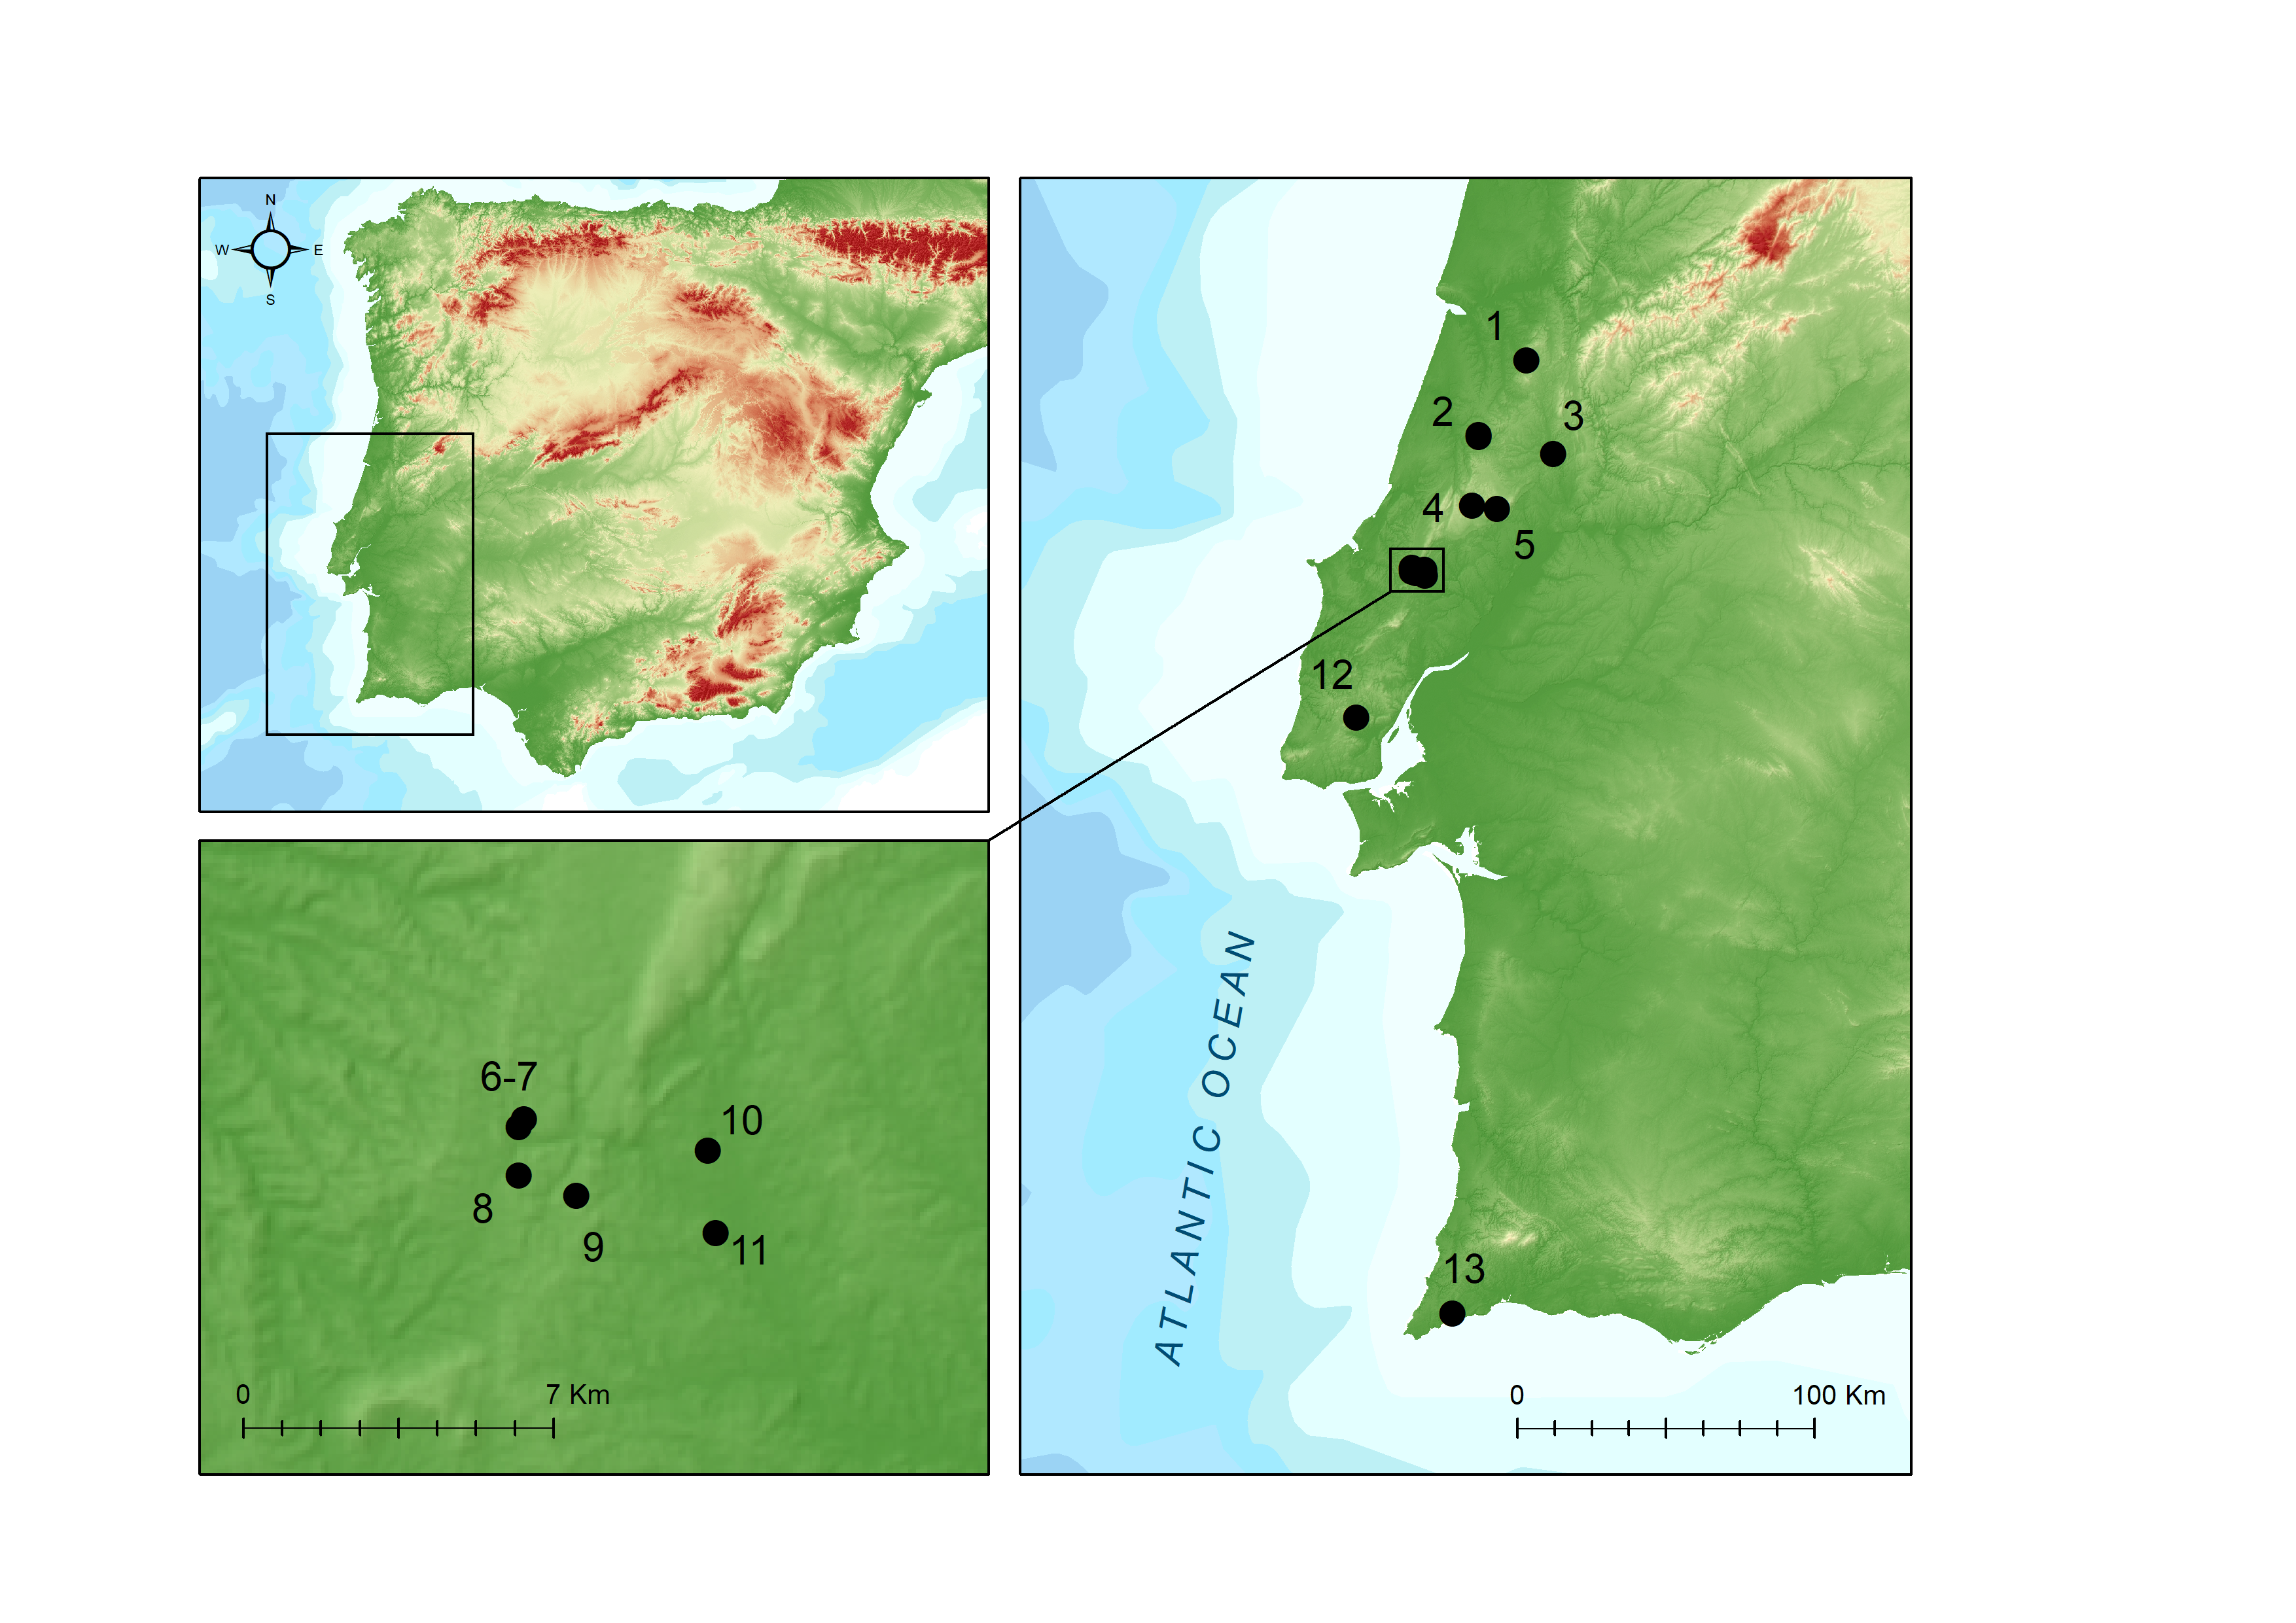
\includegraphics[width=0.5\linewidth]{figure/map_proto_solutrean} 

}

\caption{Location of Proto-Solutrean sites in Portugal, including the two sites analysed in this study.}\label{fig:protomap}
\end{figure}
The Proto-Solutrean has thus been described as a transitional techno-complex from Gravettian to Solutrean technologies, through a process of local development, and synchronous to all of the Southwestern Europe (Aquitaine, Pyrenees, Languedoc and the Iberian Peninsula) (Zilhão et al.~1999).

In total, 9 sites with either Proto-Solutrean assemblages or transitional characteristics were identified in the Portuguese Estremadura area (although not all have been dated). Table X shows the dates for Proto-Solutrean occupations in Portugal, including the sites analyzed in this study.
\begin{table}

\caption{\label{tab:unnamed-chunk-1}Summary of radiocarbon dates from Portuguese Proto-Solutrean. Adapted from Zilhão (1997), Cascalheira and Bicho (2013), Belmiro (2018) and Benedetti et al. (2019). Calibration curves are IntCal13 and Marine13, using OxCal 4.1.7 (online).}
\centering
\begin{tabular}[t]{>{\bfseries}lllrrlrr}
\toprule
Site & Level & Lab. Ref & Age (BP) & SD & Sample type & Calibrated lower 95\% & Calibrated upper 95\%\\
\midrule
LP & T & Wk-37655c & 18960 & 80 & Bone & 22620 & 23002\\
LP & T & UGAMS-23727 & 19530 & 50 & Charcoal & 23430 & 23635\\
LP & T & UGAMS-23718 & 20240 & 50 & Charcoal & 24203 & 24421\\
LP & T & Beta-208221e & 20240 & 110 & Charcoal & 24084 & 24550\\
LP & T & UGAMS-23725 & 20320 & 50 & Charcoal & 24295 & 24489\\
\addlinespace
Vale Boi & 5 & Wk-42831 & 20329 & 90 & Shell & 23763 & 24171\\
Alecrim & 6 & Beta-203513 & 20510 & 150 & Bone & 24301 & 25130\\
LP & T & UGAMS-23726 & 20530 & 50 & Charcoal & 24521 & 24905\\
LP & T & UGAMS-23722 & 20630 & 60 & Charcoal & 24600 & 25061\\
LP & T & Beta-229781e & 20700 & 100 & Bone & 24597 & 25223\\
\addlinespace
LP & T & UGAMS-23721 & 20710 & 60 & Charcoal & 24701 & 25165\\
Vale Boi & 5 & Wk-42830 & 20818 & 107 & Charcoal & 24746 & 25373\\
CPM III Inferior & NA & ICEN-541 & 21080 & 850 & Charcoal & 23346 & 27041\\
Lagar Velho & 6 & OxA-8420 & 21180 & 240 & Charcoal & 24876 & 25887\\
Lagar Velho & 6 & Sac-1561 & 21380 & 810 & Bone & 23791 & 27209\\
\addlinespace
Anecrial & 2b & ICEN-964 & 21560 & 680 & Charcoal & 24317 & 27204\\
Anecrial & 2b & OxA-5526 & 21560 & 220 & Charcoal & 25425 & 26216\\
Terra do Manuel & 2s & EHT-6038 & 21770 & 210 & Charcoal & 25661 & 26435\\
Alecrim & 6 & Wk-25514 & 21794 & 170 & Bone & 25779 & 26371\\
Buraca Escura & 2e & OxA-5524 & 21820 & 200 & Bone & 25757 & 26488\\
\addlinespace
Lagar Velho & 6 & OxA-8418 & 22180 & 180 & Charcoal & 26056 & 26935\\
Vale Boi & 5 & Wk-44416 & 22358 & 80 & Shell & 26008 & 26315\\
LP & U & Beta-234373e & 22560 & 110 & Charcoal & 26592 & 27146\\
LP & U & Beta-234374e & 22590 & 110 & Charcoal & 26623 & 27183\\
LP & U & Beta-208222e & 22660 & 240 & Charcoal & 26384 & 27384\\
\addlinespace
LP & T & Wk-37656 & 23100 & 130 & Charcoal & 27204 & 27572\\
\bottomrule
\end{tabular}
\end{table}
This set of dates from sites such as Anecrial, Terra do Manuel (layer 2s), Alecrim, Buraca Escura (layer 2e) and Lagar Velho (since other dates show either values which look like outliers or have extremely high standard deviations) place the transition as happening between 26.2 ka cal BP and 25.4 ka cal BP (calibrated dates from Zilhão 1997, using IntCal 13 through Oxcal online), where the lowest boundary represents the beginning of the Final Gravettian and the highest the ending of the Proto -Solutrean (Zilhão 1997; 2000; Zilhão et al.~1999).

The understanding of the Gravettian-Solutrean transition through several phases, each with its technological characteristics and patterns, through the techno-typological characteristics of assemblages from key sites, have allowed for the creation of two models: the Two-stage model and Three-stage model (Zilhão 1994; 1997; Zilhão et al.~1999).
\begin{figure}
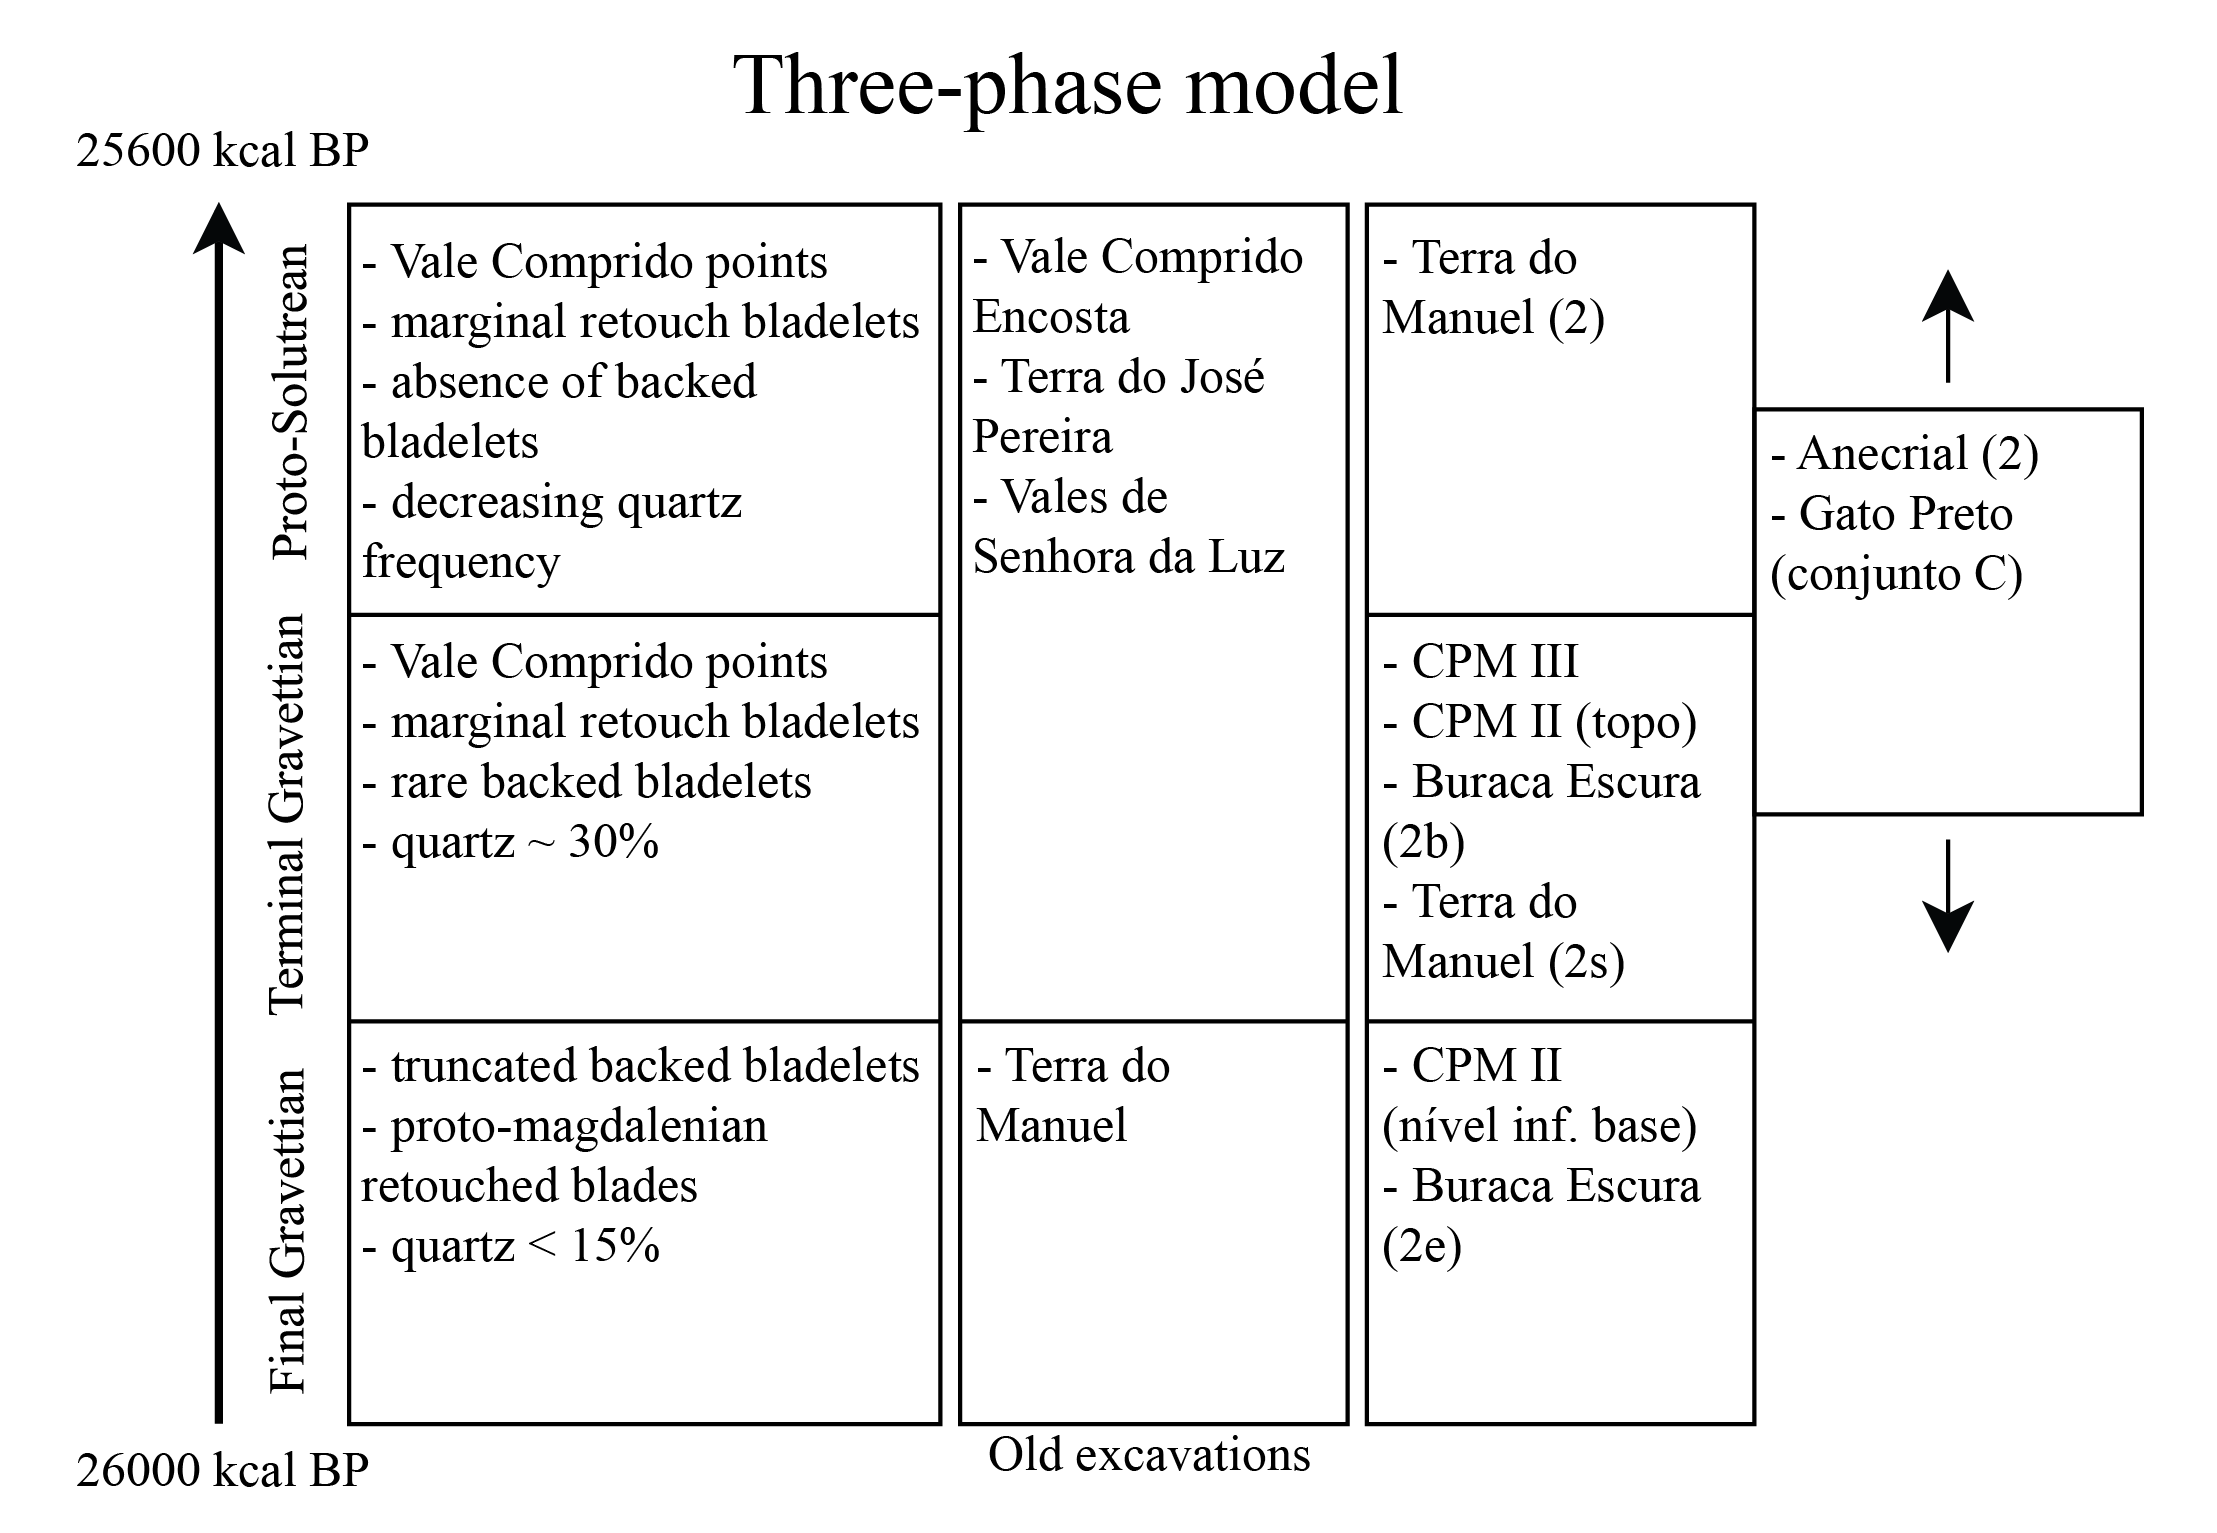
\includegraphics[width=1\linewidth]{figure/Three-phasemodel} \caption{Three-phase model for Gravettian to Proto-Solutrean transition, with site and archaeological level correlated with each phase. Adapted from Zilhão (1997). Model dates calibrated with curve IntCal13, using OxCal 4.1.7 (online)}\label{fig:unnamed-chunk-2}
\end{figure}
\begin{figure}
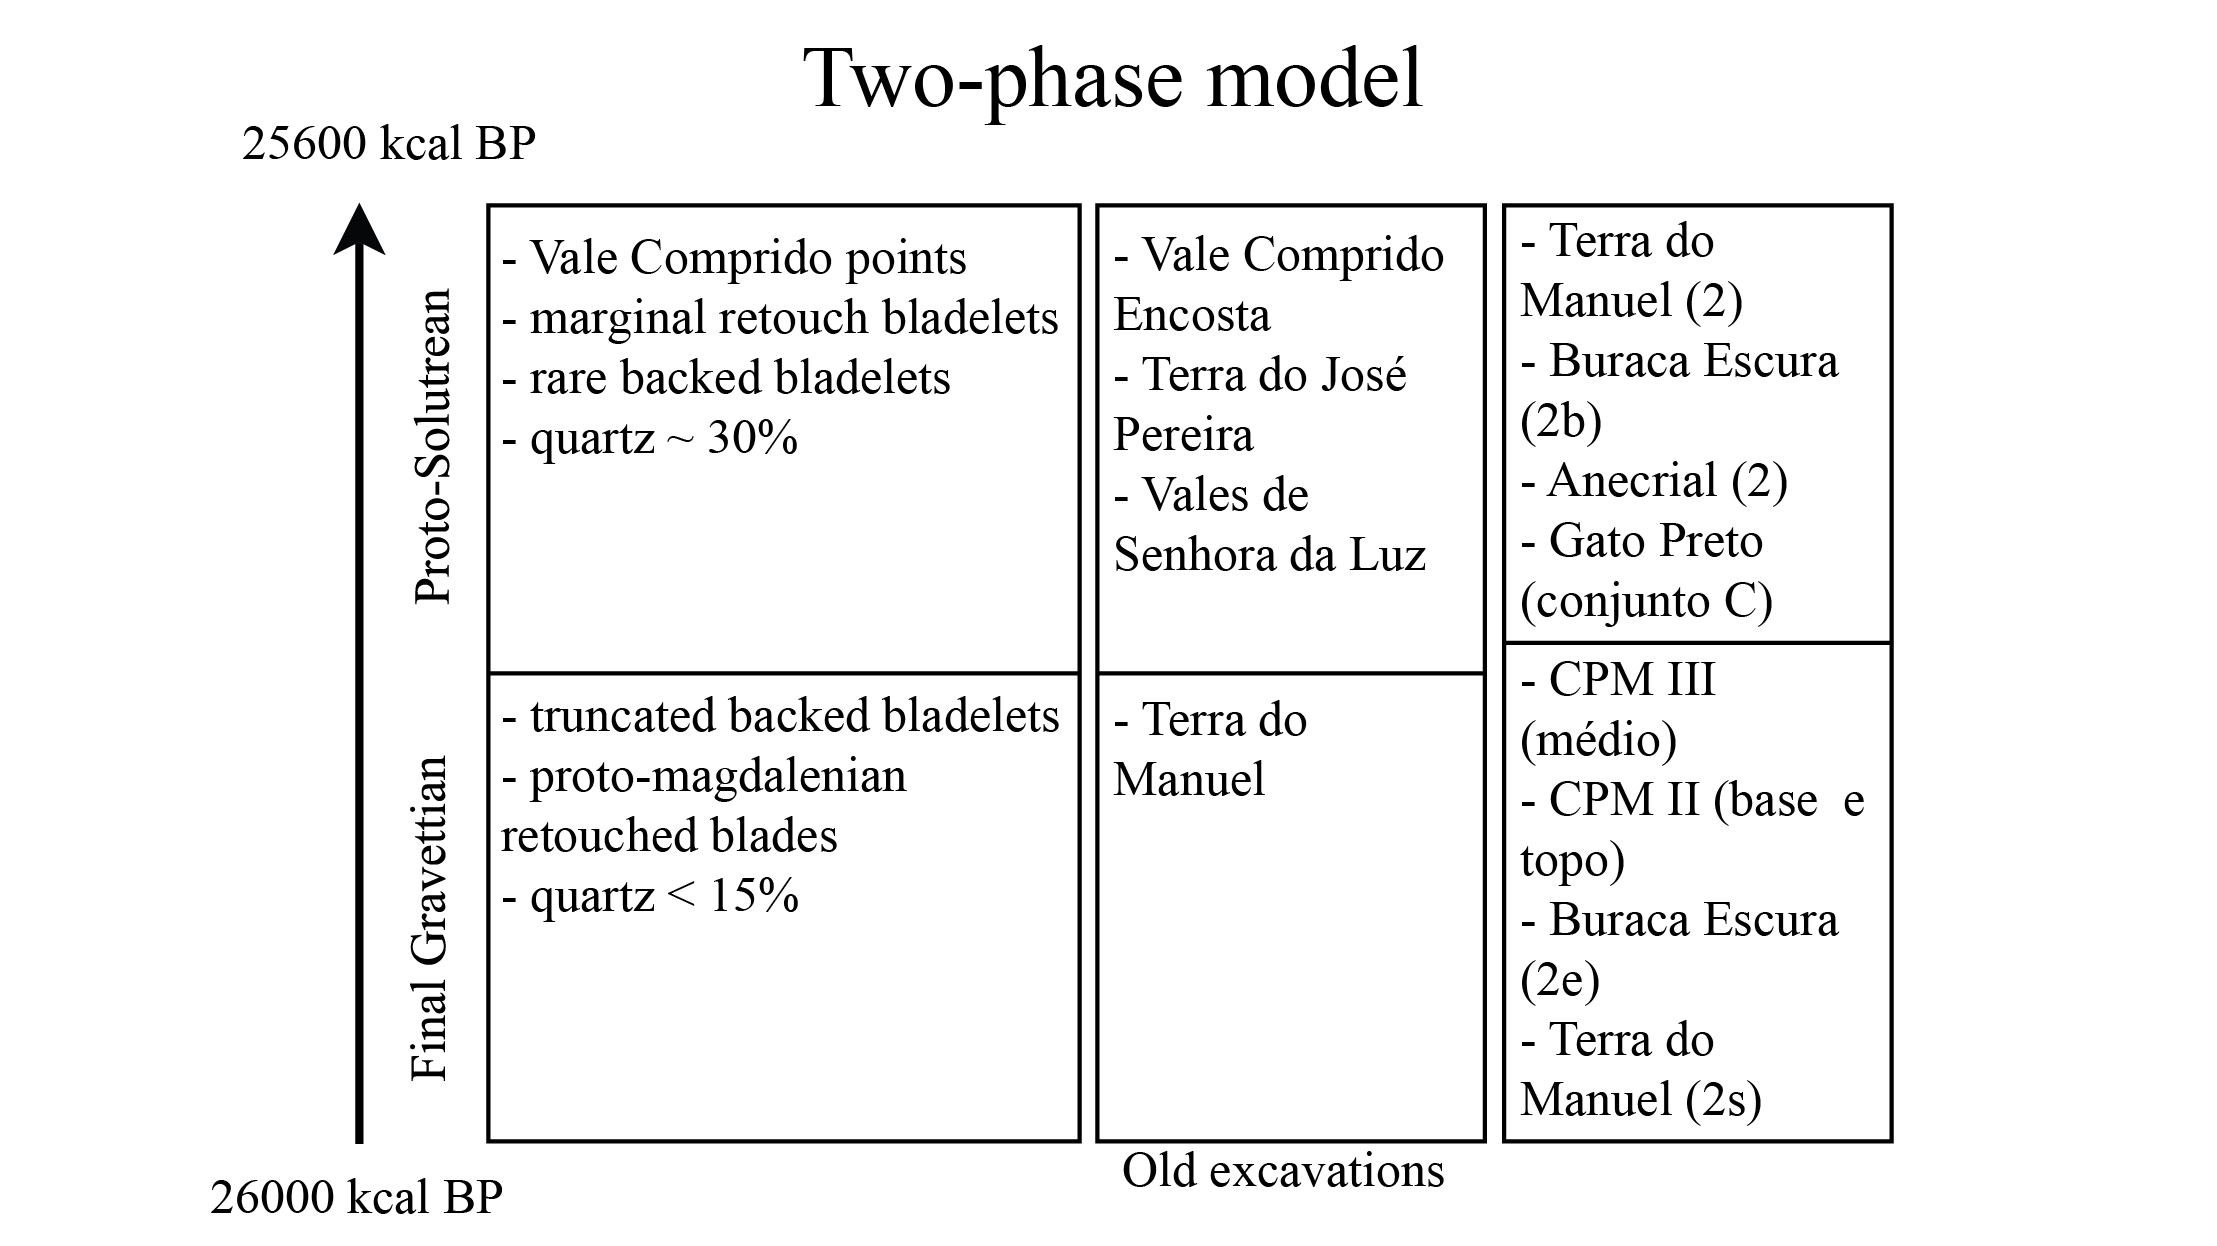
\includegraphics[width=1\linewidth]{figure/Two-phasemodel} \caption{Two-phase model for Gravettian to Proto-Solutrean transition, with site and archaeological level correlated with each phase. Adapted from Zilhão (1997). Model dates calibrated with curve IntCal13, using OxCal 4.1.7 (online)}\label{fig:unnamed-chunk-3}
\end{figure}
The Two-stage model starts with a Final Gravettian stage, characterized by a moderate use of quartz (\textasciitilde15\%), production of truncated backed bladelets and proto-magdalenian retouch blades, where we find Terra do Manuel (old excavations and layer 2s), CPM III, CPM II and Buraca Escura (layer 2e) (Zilhão 1997). The second stage is the Proto-Solutrean, frequently characterized by a high percentage of quartz use (\textasciitilde30\%), rare presence of backed bladelets and presence of marginally retouched bladelets, and the production of Vale Comprido points, the technocomplex's index fossil (Zilhão and Aubry 1995; Zilhão 1997; Almeida 2000). For the production of these tools, the Proto-Solutrean shows three different operative sequences: one destined to the production of Vale Comprido points, through the removal of elongated blanks with convergent profiles and thick platforms; another destined to the production of blades, of Gravettian tradition; and another for the production of bladelets, probably obtained through the exploitation of thick endscapers. Proto-Solutrean phase assemblages were identified in Vale Comprido -- Encosta, Terra do José Pereira, Vales da Senhora da Luz (although Vale Comprido points are absent from the assemblage), Terra do Manuel (layer 2), Buraca Escura (layer 2b), Anecrial (layer 2) and Gato Preto (group C) (Zilhão 1997).

Vale Comprido points are described as robust pieces, with a thickness ranging the 4-8 mm, width around 20 mm and length of about 50mm, though in some cases it may reach 80 mm, and platform thickness of 5-20 mm. They are often characterised by convergent shapes, triangular cross- sections and plain platforms, often having a high elongation ratio, although not necessarily falling into the blade category. They can also be categorized regarding retouch, with the identification of 3 groups: 1) point with thinning of the platform; 2) marked by extensive retouch across the edges, including the tip; 3) an intermediate type with only partial retouch on the edges along the platform or at the tip \{Zilhão (1997); ZILHÃO \& Aubry (1995)\}. The Vale Comprido points have been used to describe the technological transition between the Proto-Solutrean and the Solutrean. In this case, these points are seen as an element of discontinuity with the previous technocomplex, where the organic points armed with microliths from the Gravettian are replaced by lithic points, with enough similarities to the pointes à face plane of the Middle Solutrean to be understood as a technological development \{Zilhão (2013)\}.

The Three-stage model maintains the first Final Gravettian stage and its defining characteristics but subdivides the following Proto-Solutrean stage in two. As such, there is an intermediate stage characterized by the intensive use of quartz (\textasciitilde30\%), which corresponds to Laugerie Haute's ``Aurignatian V'', migrating the assemblages from Terra do Manuel (layer 2s), CPM III, CPM II and Buraca Escura (layer 2b) to this phase, with a third stage, the Proto-Solutrean, where quartz use diminishes and there is an important presence of carinated elements for the production of bladelets, mostly visible at Terra do Manuel (layer 2). In this model, the Vale Comprido points and associated reduction sequence may appear in either of the last two stages, although it is probable that the technology was developed during the transition to the intermediate stage (Zilhão 1997).

Alternatively, in the Two-phase model, the ``Aurignacian V'', is understood as a functional facies, related to specialized occupations and production activities within the techno-complex, through the observation of the coexistence of prismatic core exploitation and carinated core exploitation, both for the extraction of blades and bladelets, thus showing the latter exploitation was not an independent system as thought at Laugerie Haute (Zilhão and Aubry 1996; Zilhão 1997). In fact, Zilhão (1994; 1997) has questioned the stratigraphic reality of ``Aurignacian V'' from Laugerie-Haute, interpreting it as only a typology separation due to poor stratigraphic integrity.

Almeida (2000) interprets the diagnostic Aurignacian thick-nosed endscrapers as carinated cores, with no correlation to the Aurignacian techno-complex, suggesting instead the substitution of the term Aurignacian V for Terminal Gravettian. Following previous works (Almeida 2000; Cascalheira and Bicho 2013; Benedetti et al.~2019), when referring to the ``Aurignacian V'', whether as a functional facies (Two-stage model) or as an intermediate stage (Three-stage model), the present study will apply the term Terminal Gravettian instead.

One of the main differences between the models mentioned above is connected to the lithic assemblage's internal variability. In this case, the Three-stage model diminishes this internal variability by attributing chronological significance to the Terminal Gravettian (Almeida 2000). While the Three-Phase model causes some sites to float between the Terminal Gravettian and Proto-Solutrean without an exact phase attribution (such as Terra do José Pereira, Vales da Senhora da Luz, Anecrial and Gato Preto), due to lack of necessary information or specialized character of their occupations \{Zilhão (1997)\}, the Two-phase, because it accepts higher internal variability but also limits the number of options, guarantees that a specific phase can be attributed to all sites.

However, in the last decades, the Three-Phase model has been the most accepted, and the Terminal Gravettian phase is nowadays well-characterized technologically in Estremadura as a moment of chronological significance (Almeida 2000), even if from a chronographic perspective, it lacks irrefutable evidence as shown by Cascalheira and Bicho (2013), for which the authors present two causes: all available radiocarbon dates, spreading through the entire HE2 and covering the Proto-Solutrean's time-span, come from sites whose assemblages are attributed to the Terminal Gravettian (with the exception of Vale Boi); absolute ages of sites with a strong Vale Comprido component remain unknown.
Although this has been explained by some authors (e.g.~Aubry et al.~2011; Zilhão 2013) as the result of strong erosive processes affecting the archaeological sites during the HE2, other authors (Haws 2012) fail to recognize such an extensive erosion.

Regardless of what model is accepted, the Proto-Solutrean, from the beginning of its transitional stage, stands as a techno-complex with technological innovations, reflected in the manufacture of Vale Comprido points and a complete operative sequence for their production, but marked by a high degree of technological variability in their lithic assemblages (Zilhão 1997; Zilhão et al.~1999; Almeida 2000).

This variability has been interpreted as a technological race in response to the environmental modifications taking course during the HE2 (Cascalheira and Bicho 2013). The authors suggest that, in order to correspond to the external pressures, there may have been the need to diversify the economic strategies in use until that moment. The high exploitation of quartz, for example, formerly a secondary raw material, and the use of similar reduction strategies between quartz and chert, might represent one such economic response. The same possibly applies to the use of unprecedented raw materials for specific products, as is the case of the Proto-Solutrean levels in Vale Boi, where there is the presence of previously unknown raw materials, used mainly in the manufacture of Vale Comprido points (Marreiros 2009; Belmiro 2018). Likewise, alterations recorded in territoriality patterns for the Proto-Solutrean, which can be interpreted has extensive regional networks, may also be related to modifications in the landscape that occurred during the HE2 (Cascalheira and Bicho 2013).

These technological and behavioral changes, when understood under the light of the Repeated Replacement Model previously discussed (Brädmoller et al.~2011) and Panarchy (Holling and Gunderson 2003), might be understood as moments of release and restructuration led by external pressures, in this case, climate changes (Cascalheira and Bicho 2013).

Thus, following this framework, the Proto-Solutrean reveals itself as a moment of ``creative destruction'' (Holling 2001), with moments of rupture and consolidation of technological innovations and social structures. In other words, the Proto-Solutrean might be understood as the moment where Gravettian cultural traditions were reconfigured to best adapt to climatic and landscape alterations, setting grounds for the emergence of another phase -- the Solutrean (Cascalheira and Bicho 2013).

However, despite the existence of rather comprehensive knowledge about the techno-complex in the Portuguese Estremadura, which has allowed for a better understanding of the impacts of HE2 in hunter-gatherer communities and the emergence of the Solutrean, there is still the need for further studies, in order to fill existing gaps. One of these gaps is the concentration of data regarding this techno-complex in the Estremadura, whereas the Proto-Solutrean is still relatively unknown in other places throughout Southwestern Europe, in the case of Portugal, with only one site in the south (image x). Another issue, which has been mentioned already, is connected to the absence of absolute datings for Proto-Solutrean contexts, which limits the chronological definition of the techno-complex, and thus the testing of which transition model (if any) applies best (Cascalheira and Bicho 2013).

Addressing these issues, through the study of Proto-Solutrean lithic assemblages from other areas in the Southwestern European territory, from sites with good stratigraphic preservation which allow absolute dating and accurate spatial tracking, will undoubtedly help further understand this techno-complex, its patterns, stage transitions and possible regional variations.

\hypertarget{location-and-geological-context}{%
\chapter{Location and geological context}\label{location-and-geological-context}}

\hypertarget{vale-boi}{%
\section{Vale Boi}\label{vale-boi}}

Vale Boi is an open-air site and rockshelter, located on the western coast of Algarve (Portugal), near a small homonymous village, within the municipality of Vila do Bispo. The site is situated in a small valley that runs south to the Atlantic coast, about 2 km distance, relatively open, with a natural boundary to the East and bordered by a limestone hill through all its extension. This hill is marked, at specific points, by limestone exposures that form rock shelters with faces facing west or southwest (Bicho et al.~2003; Cascalheira et al.~2008; Cascalheira 2010).
\begin{figure}

{\centering 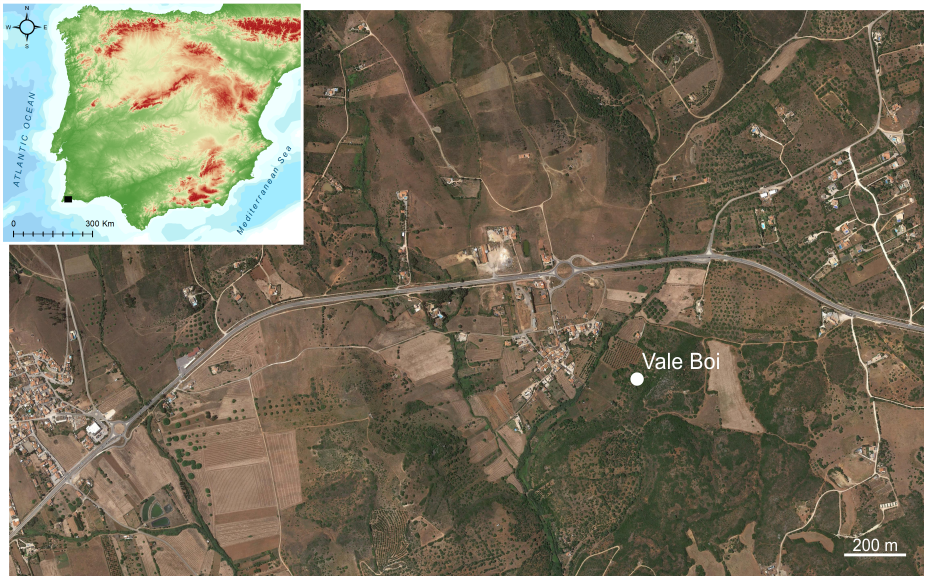
\includegraphics[width=0.5\linewidth]{figure/vale_boi_map} 

}

\caption{Location of Vale Boi.}\label{fig:vbmap}
\end{figure}
The site extends for more than 10 000 m2 on the slope of this valley, which is marked by a series of steps that run parallel to the river, possibly the result of Middle Pleistocene fluviatile erosion (Bicho et al.~2003).
\begin{figure}

{\centering 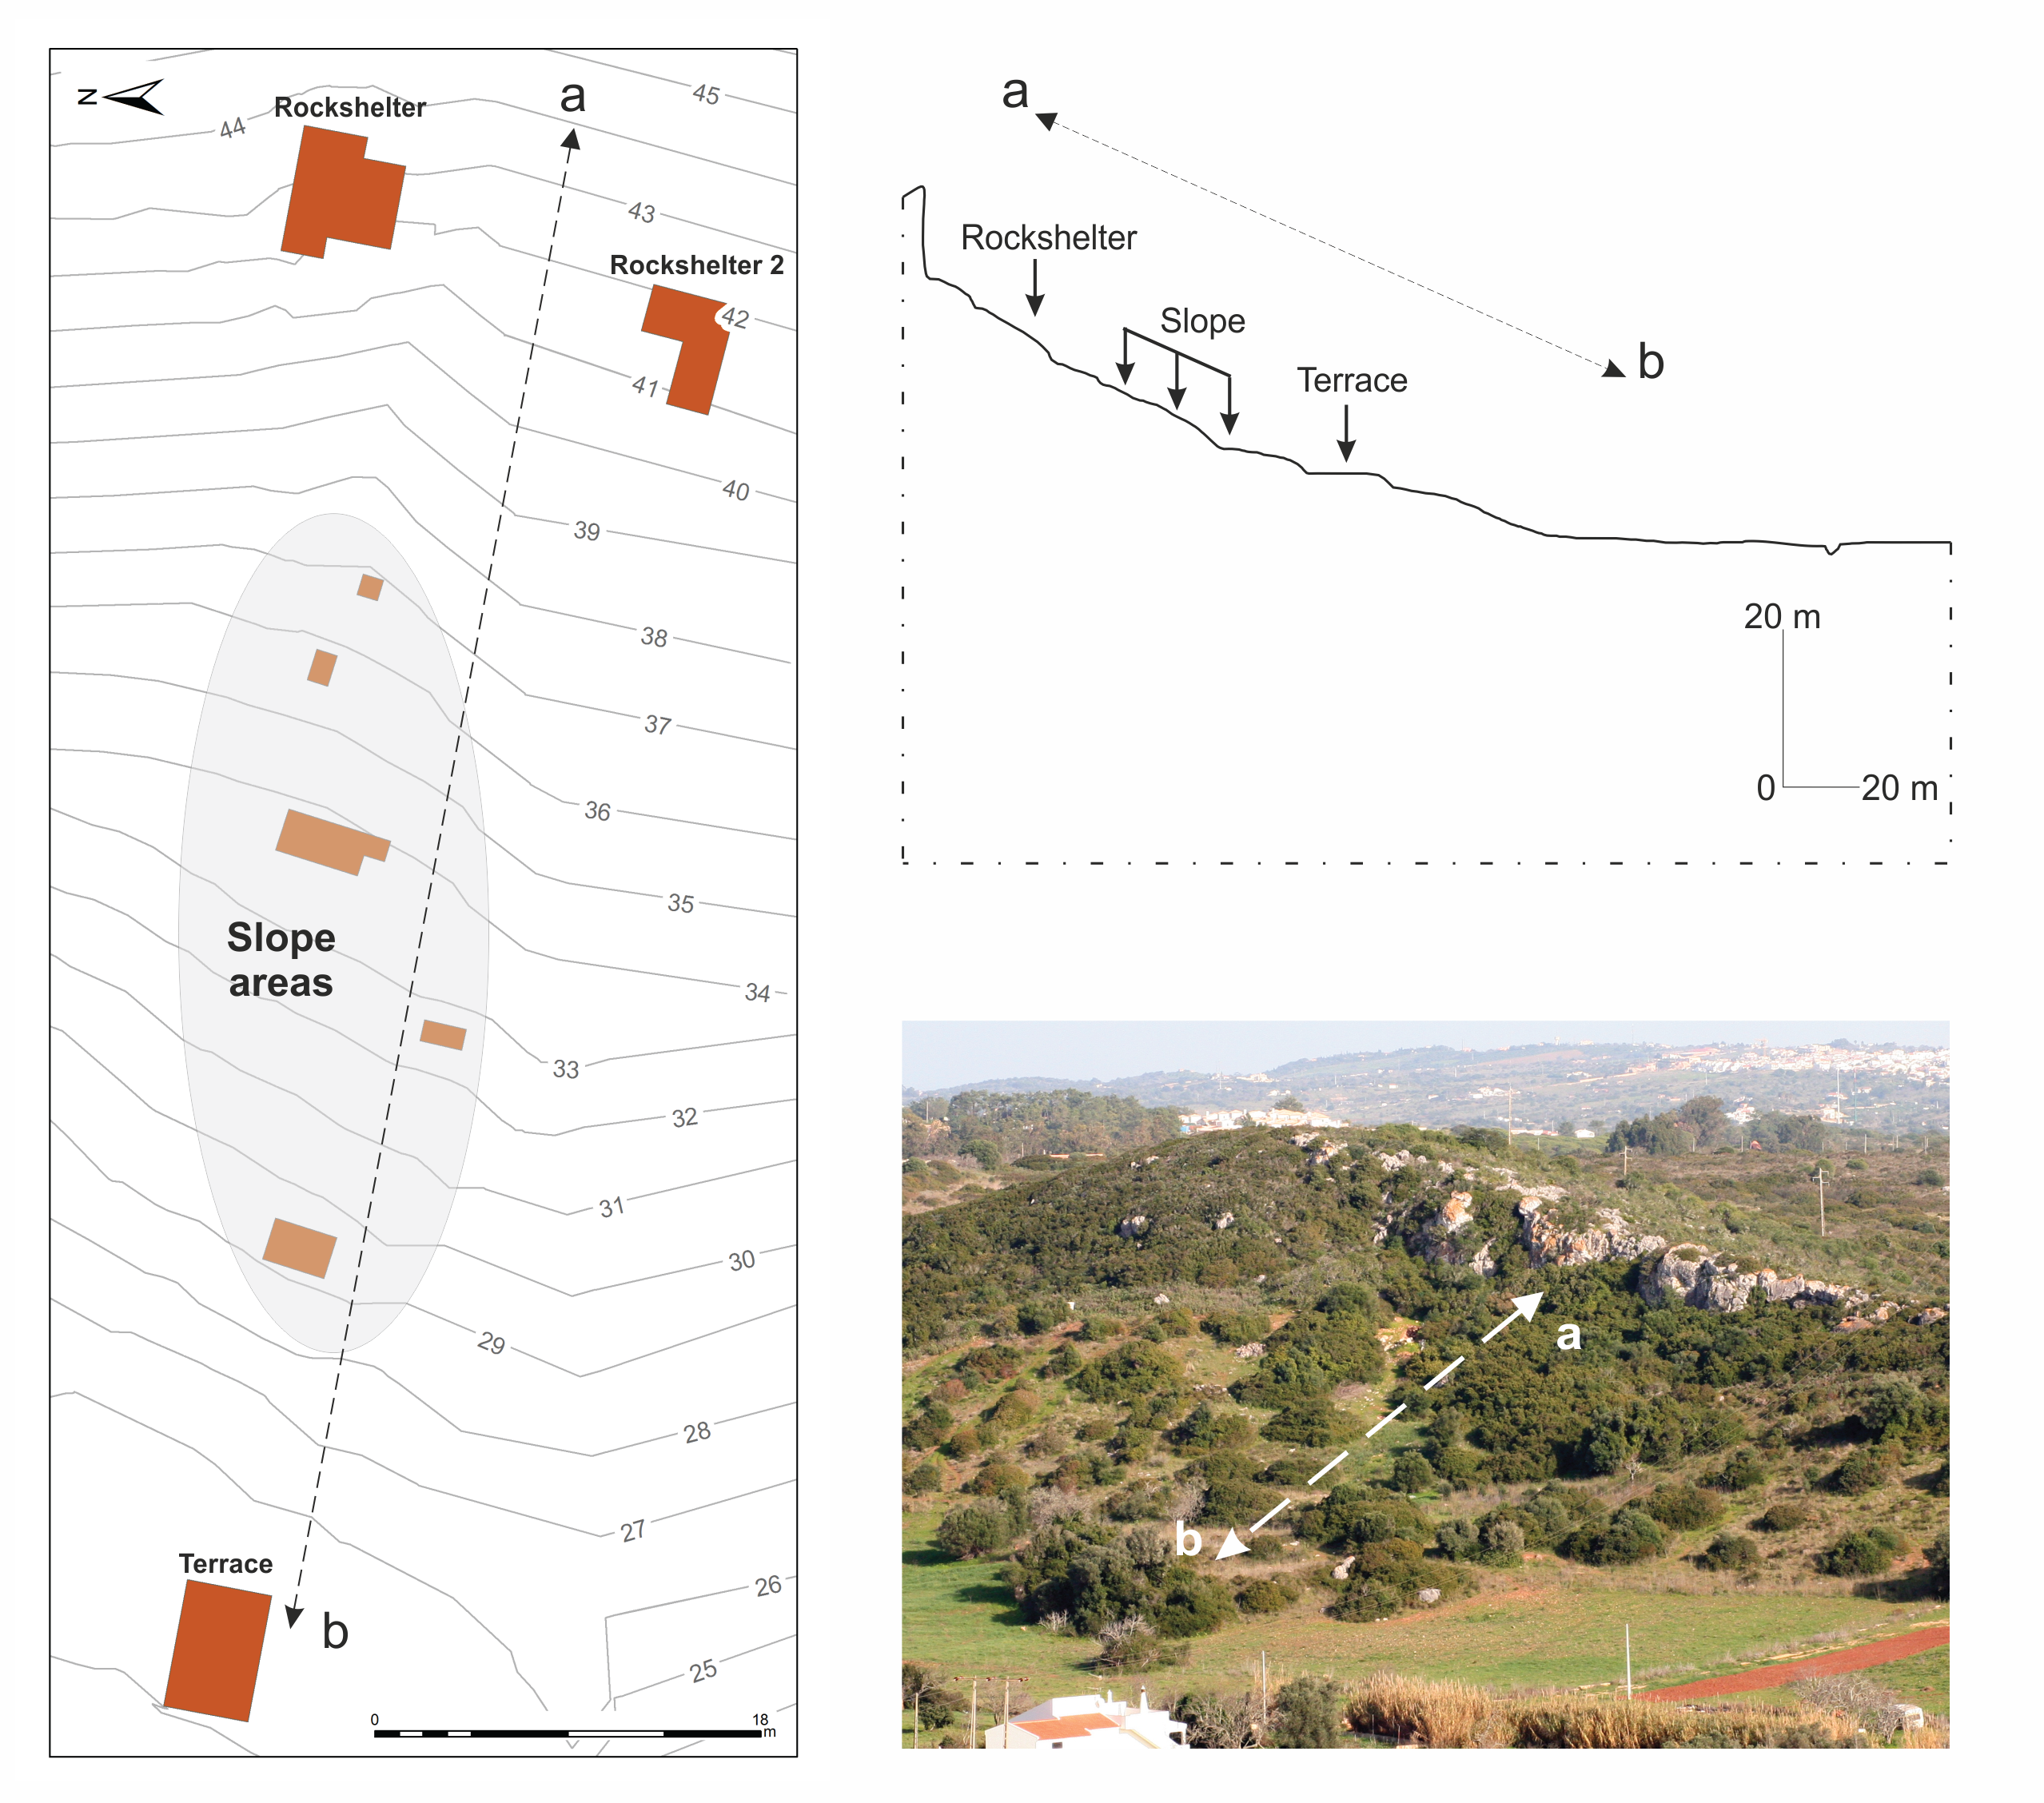
\includegraphics[width=0.5\linewidth]{figure/vb_plan} 

}

\caption{Topographic plan, schematic profile and general view of Vale Boi, with location of the excavation loci. After Cascalheira et al. 2017.}\label{fig:vbphoto}
\end{figure}
The geologic context of Vale Boi is marked by heterogeneity. In the north, there are schist and greywacke formations from the Carboniferous, and in the south, Triassic and Jurassic dolomite and limestone formations, which are gradually covered by Holocene dunes further into the coastal area, until near St.~Vincent's cape where they appear uncovered once again, along with small occurrences of chert (Veríssimo 2004).

\hypertarget{lapa-do-picareiro}{%
\section{Lapa do Picareiro}\label{lapa-do-picareiro}}

Lapa do Picareiro is a cave site on the west facing slope of Serra d'Aire, a limestone massif north of the Tagus River valley and Lisbon, Portugal (Benedetti, Haws, Bicho, Friedl, \& Ellwood, 2019; Bicho, Haws, \& Hockett, 2006). The massif is underlain by the Serra d'Aire Formation, a thick-bedded limestone of the Middle Jurassic age (Carvalho, 2018). The Serra d'Aire is part of a large limestone province (Maciço Calcário Estremenho), which accounts for several Palaeolithic occupations, both cave and open-air sites (Almeida, 2000; Benedetti et al., 2019).

The cave appears to have an epigenetic origin, formed by infiltration of meteoric water through the overlying bedrock leading to the dissolution of the main chamber and roof collapse which formed the cave entrance (Benedetti et al., 2019). The interior of the chamber is about 11 x 14 m, and has more than 10 m of coarse sedimentary infill in inclined beds, derived from roof collapse, gravity flows and fine sediment infiltration (Benedetti et al., 2019). The cave opening is marked by the existence of a cone of large limestone stone blocks (Bicho et al., 2006) while the sediment inside the cave consists of smaller and angular limestone clasts in a matrix of fine sediment (Benedetti et al., 2019).
\begin{figure}
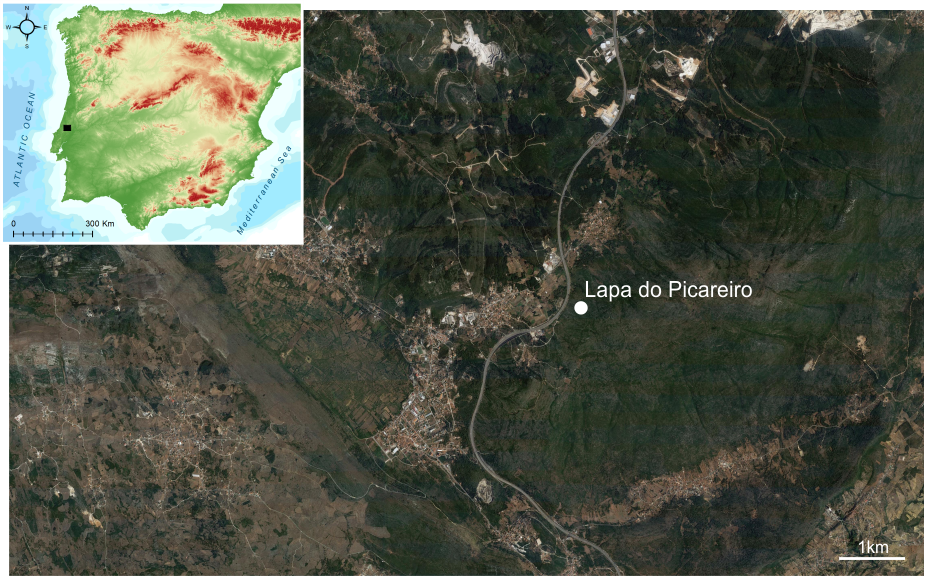
\includegraphics[width=1\linewidth]{figure/picareiro_map} \caption{Lapa do Picareiro location.}\label{fig:unnamed-chunk-4}
\end{figure}
\begin{figure}
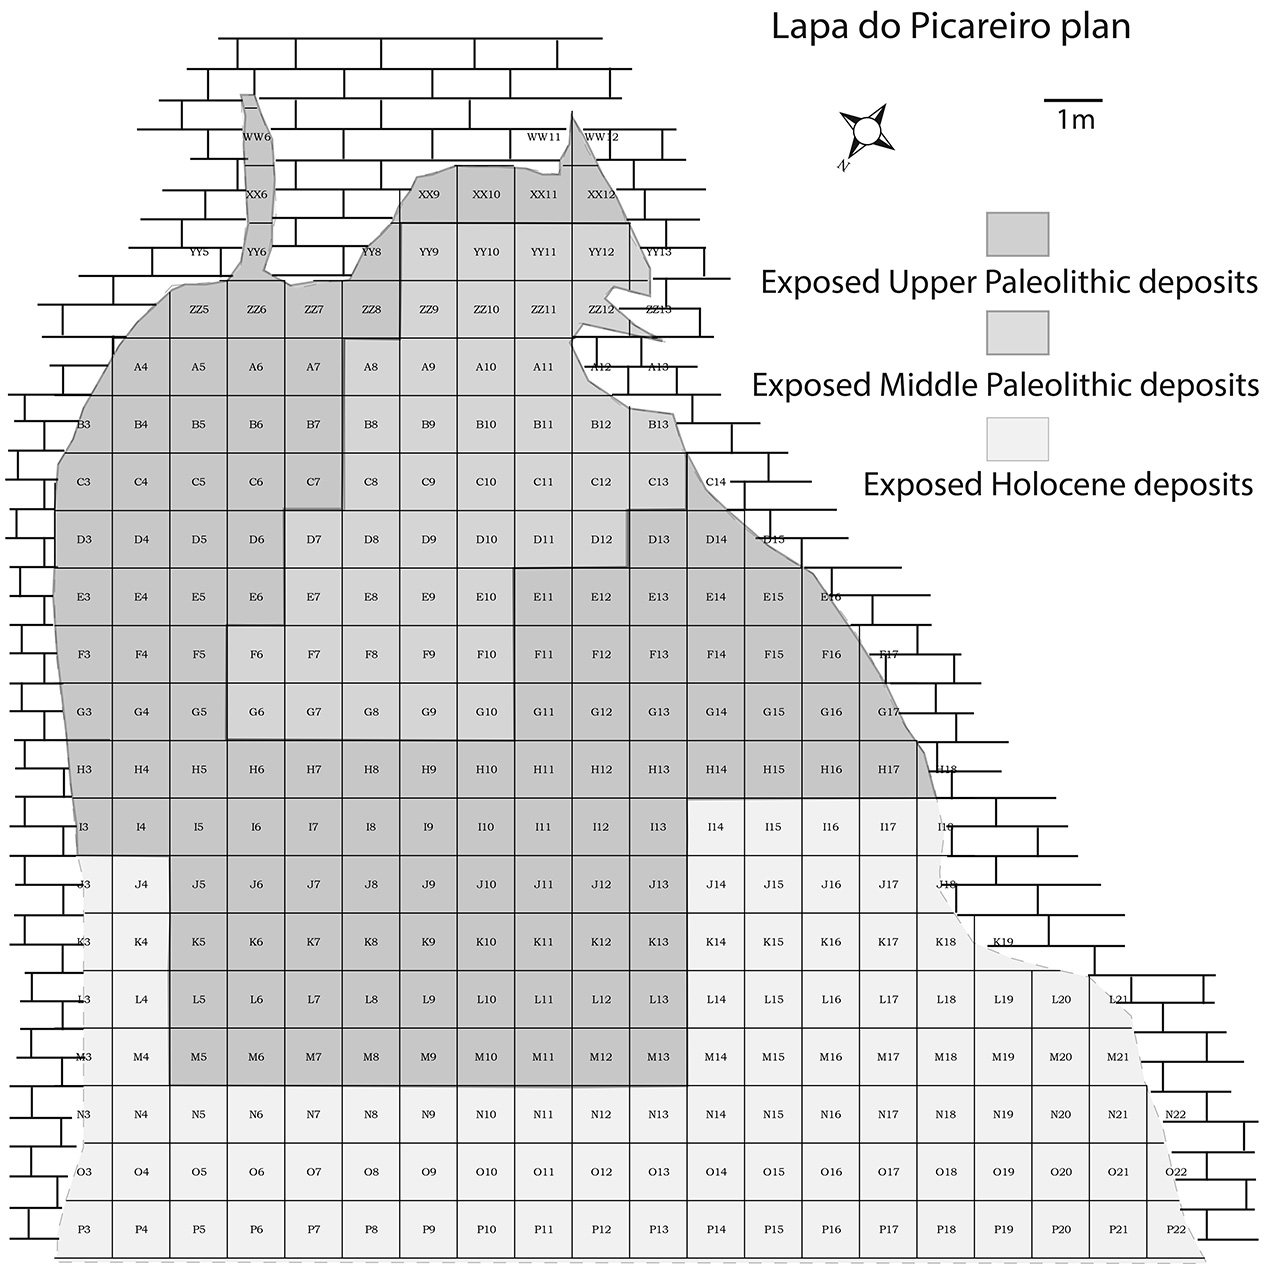
\includegraphics[width=1\linewidth]{figure/LP_units} \caption{Lapa do Picareiro generalized cross section showing surface topography, shape of the cave, and area excavated into sedimentary fill (after Benedetti et al, 2019).}\label{fig:unnamed-chunk-5}
\end{figure}
\hypertarget{research-history-stratigraphy-and-human-occupation}{%
\chapter{Research history, stratigraphy and human occupation}\label{research-history-stratigraphy-and-human-occupation}}

\hypertarget{vale-boi-1}{%
\section{Vale Boi}\label{vale-boi-1}}

Vale Boi was firstly discovered as the result of a multidisciplinary project (A ocupação Humana Paleolítica do Algarve) developed in 1996, led by Nuno Bicho and funded by the Fundação para a Ciência e Technologia (FCT), with the goal of characterizing the regional Paleolithic and Epipaleolithic, building an absolute chronology for the pre-historic sequence in the Algarve, and motivated by the lack of known Paleolithic sites in this region (Cascalheira 2010). Through ground reconnaissance and the opening of test pits, the project focused on the areas with higher potential for Paleolithic occupations (specifically in what concerns to topography, access to natural resources such as fresh water, proximity to raw materials, proximity to specific geologic units) (Bicho et al.~2003). Sixty-five archaeological sites were identified, 7 with identifiable Gravettian, Solutrean and Magdalenian occupations, from which Vale Boi offered the best results (Cascalheira 2010). For this reason, the site has been systematically excavated and has had several funded projects (e.g.~``A importância dos recursos aquáticos no Paleolítico do Algarve'' and ``História de dois mares: ecologia do Paleolítico Superior em Vale Boi'').

The archaeological interventions started in 2000, with the opening of several units on the slope area, where there was a significant concentration of archaeological materials at the surface, and where the topography seemed adequate for the preservation of in situ materials. From 2002 onwards, some of these excavation units were expanded, aiming to identify the extension of the site (Cascalheira 2013).

In 2003, new excavation units were open on the west and east limits of the site, which led to the excavation of another two areas, the Shelter and the Terrace, that would be incrementally expanded through the following years.

In 2012, a new 8 square meters area was open in the Terrace (rows H and I), to understand the stratigraphic sequence in more detail, and assess the existence of older cultural horizons, from the early Upper Paleolithic.

Vale Boi shows a variety of human occupations, distributed across three main areas, which have been interpreted differently in terms of functionality: Slope, Shelter, and Terrace (fig x).

\hypertarget{slope}{%
\subsection{Slope}\label{slope}}

In this area, three moments of occupation have been identified, although the first layer seems to be very altered, with only the presence of sorted, small lithics and no associated fauna. This layer corresponds to a Magdalenian occupation. The other levels, however, seem to be in situ, since there were faunal remains in anatomical position, the presence of stacked, well preserved, shells and general horizontal disposition of the materials, without size sorting, which often happens through pluvial action (Bicho et al 2003).

The Solutrean occupation is characterized by bigger lithics than those found in the layer above, abundant animal bones and shells, with relatively less rabbit than the layer below. This layer is also marked by a moment of geological discontinuity through the presence of a large number of limestone blocks and pebbles (which are probably related to the start of the Last Glacial Maximum, and where Proto-Solutrean materials were found, including a Vale Comprido point (Cascalheira 2010).

Bellow the discontinuity, there is a Gravettian occupation, with a more significant number of artifacts, specifically a high number of ornaments of Littorina obtusata and deer teeth, as well as at least 12 identified bone tools (Cascalheira 2010).

This area has been interpreted as a midden, the result of waste produced by several human activities, such as the production and maintenance of lithic artifacts, preparation of food, and carcass treatment (Bicho et al 2003).

\hypertarget{shelter}{%
\subsection{Shelter}\label{shelter}}

The occupation levels in this area were located under blocks of limestone, which collapsed from the rockshelter ceiling, and where occupations of Magdalenian, Solutrean, and Gravettian chronologies have been identified across four distinct litho-stratigraphic units.

A small combustion structure was identified in this area, within the Solutrean layers. This structure was circular, with around 50 cm of diameter, formed by limestone pebbles and blocks. The area around the fireplace was marked by calcination, where several artifacts were found with thermal alterations (Cascalheira et al 2008).

The shelter has been interpreted as a residential space, differing from the previous area, especially in the representation of the stone tool reduction sequences, the preservation of the bones, which are less fragmented, the diversity of shells used as ornaments and the presence of a decorated schist plaque, thus pointing towards the use of the shelter as a daily camping area (Cascalheira 2010).

\hypertarget{terrace}{%
\subsection{Terrace}\label{terrace}}

As previously mentioned, excavations in the Terrace area started in 2003. The identification of two human occupation levels and a possible limestone block pavement led to the area's expansion, in the following year, towards the south and western boundaries. This expansion allowed the identification of a hut pavement attributed to the Early Neolithic based on the recovered ceramics and lithic materials (Carvalho 2008).

Excavations on the Pleistocene levels of the area started in 2004/05 (Marreiros 2009; Cascalheira 2010), intending to find Paleolithic habitat structures (Cascalheira et. al 2008), and allowed the identification of two different layers, marked by an intermediate moment of geologic discontinuity. While the upper layers showed materials attributed to the Solutrean, the bottom levels allowed the identification of a Gravettian occupation (Cascalheira 2010; Marreiros 2009). In this latter horizon, in 2007, a combustion structure was identified, adjacent to the north wall. This structure was characterized by an ovoid shape, achieved by the combination of small limestone blocks with what seemed a larger repurposed block, and was full of burnt organic remains as well as large quantities of charcoal, in association with lithic materials (Cascalheira 2010).

Thus, the excavation in this area (units J, K and L) allowed for the identification of 4 layers: layer 1, marked by ceramics and possibly disturbed by agricultural works; layer 2, characterized by the Neolithic occupation mentioned above; layer 3, which corresponds to several Solutrean occupation levels; and layer 4, with two human occupations attributed to the Gravettian technocomplex (Marreiros 2009).

After 2012, the Terrace area was extended, with the opening of two new rows, H and I (in a total of 8 m2). Since then, six layers have been identified (table X containing the description of their sediment characteristics and associated cultural horizons). In some of these layers, lateral sediment variations were identified, which were coded in the field through the concatenation of a letter to the layer number (e.g.~4E). In many of these cases, the isolation of this vertical variation did not show any patterns in terms of spatial concentration of materials, although in others, like the 4E facies, the subdivision of the layer correlated with the spatial distribution of Vale Comprido technology.

In the new area, layers 1 and 2 continue to represent Holocene levels, with the first layer being possibly disturbed by agricultural processes, while layer 2, with a thickness of 25-30 cm, in concordance with the excavations prior to 2005, shows a Neolithic occupation.

Layer 3 has a silt and clay matrix sediment, with some inclusions and showing interruptions of limestone clasts depositional episodes, although there is the constant presence of fauna and lithic artifacts. As mentioned above, the different material and cultural characteristics within the same geologic package led to the subdivision of the layer in 3A, attributed to an Epipaleolithic occupation, and 3B, assigned to the Solutrean.
Layer 4 is very similar to layer 3. However, it is separated from it by a gravel layer. Similarly to layer 4, these layers have been subdivided regarding different degrees of sediment compaction and/or concentration of organic materials, showing two differing cultural horizons: Solutrean and Proto-Solutrean (limited to layer 4E).

Layer 5 has a dark coloration and a silt and clay matrix characterized by an intense presence of organic elements, frequently calcinated. There is the presence of a Proto-Solutrean horizon within the top levels, although occupation intensity seems to diminish with depth (see Chapter XXX).

Finally, layer 6 is very similar to the previous layer, although it shows the presence of a larger quantity of small and medium-sized limestone clasts. A Gravettian horizon has been attributed to this layer, but the analysis of the materials is currently in progress.

Regarding layers 4E and 5, although they are indeed layers with different sedimentary packages, they show similar technological and archaeological patterns, which led to the conclusion they were the same cultural horizon (the opposite, one single layer with different cultural horizons is equally present in the Terrace, as seen with the Epipaleolithic and Solutrean occupations of layer 3). These layers, 4E and 5, are vertically contiguous, separated by a relatively flat surface covered by large limestone blocks. Unlike what was expected, however, these levels did not reveal a Gravettian assemblage with characteristics similar to previous years (Marreiros 2009), but rather materials with patterns similar to those expected in a Proto-Solutrean assemblage (the most noticeable of all being the Vale Comprido points and blanks). The context was dated using a charcoal sample to c.~24.7-25.3 kcal BP, and a shell sample to c.~23.7-24.1 kcal BP.

The bottom spits of layer 5, on the other hand, show a relatively dense concentration of Littorina littoreia, an unprecedented shell species at the site, and often associated with colder waters, having a high freezing tolerance (Murphy 1979). This context was dated through a shell sample, showing dates ranging between the 26-26.3 kcal BP, which corresponds to the first half of the HE2 (Sanchez-Goñi and Harrison 2010).

Figure X represents the vertical distribution of all piece-plotted lithics in the Terrace, rows H and I. One of the most noticeable features is the vertical constraint in the distribution of dolerite pieces, mostly concentrated on layer 4E and upper levels of 5, coinciding also with the higher concentration of lithic materials in these layers. Likewise, the presence of Vale Comprido points is also associated with the top levels of layer 4E and 5 (Belmiro in press), which coincide with the dates that range from c.~23.7 to 24.7 ka cal BP (lower calibrations). As mentioned in Chapter XXX, these dates seem to fall outside the timeframe for the Proto-Solutrean as defined by Zilhão (1997) for the Portuguese Estremadura, extending it as much as nearly 2 ka years, and thus, hinting that the Proto-Solutrean at Vale Boi might have either happened later or lasted longer than has been argued for Central Portugal. The WK-44416 date, however, seems to show that, at least from around c.~26 ka cal BP, the site was occupied even if at a lower intensity, a date that falls onto the Final Gravettian/Proto-Solutrean or Final Gravettian/Terminal Gravettian transition in the traditional models (Zilhão 1997).
\begin{figure}
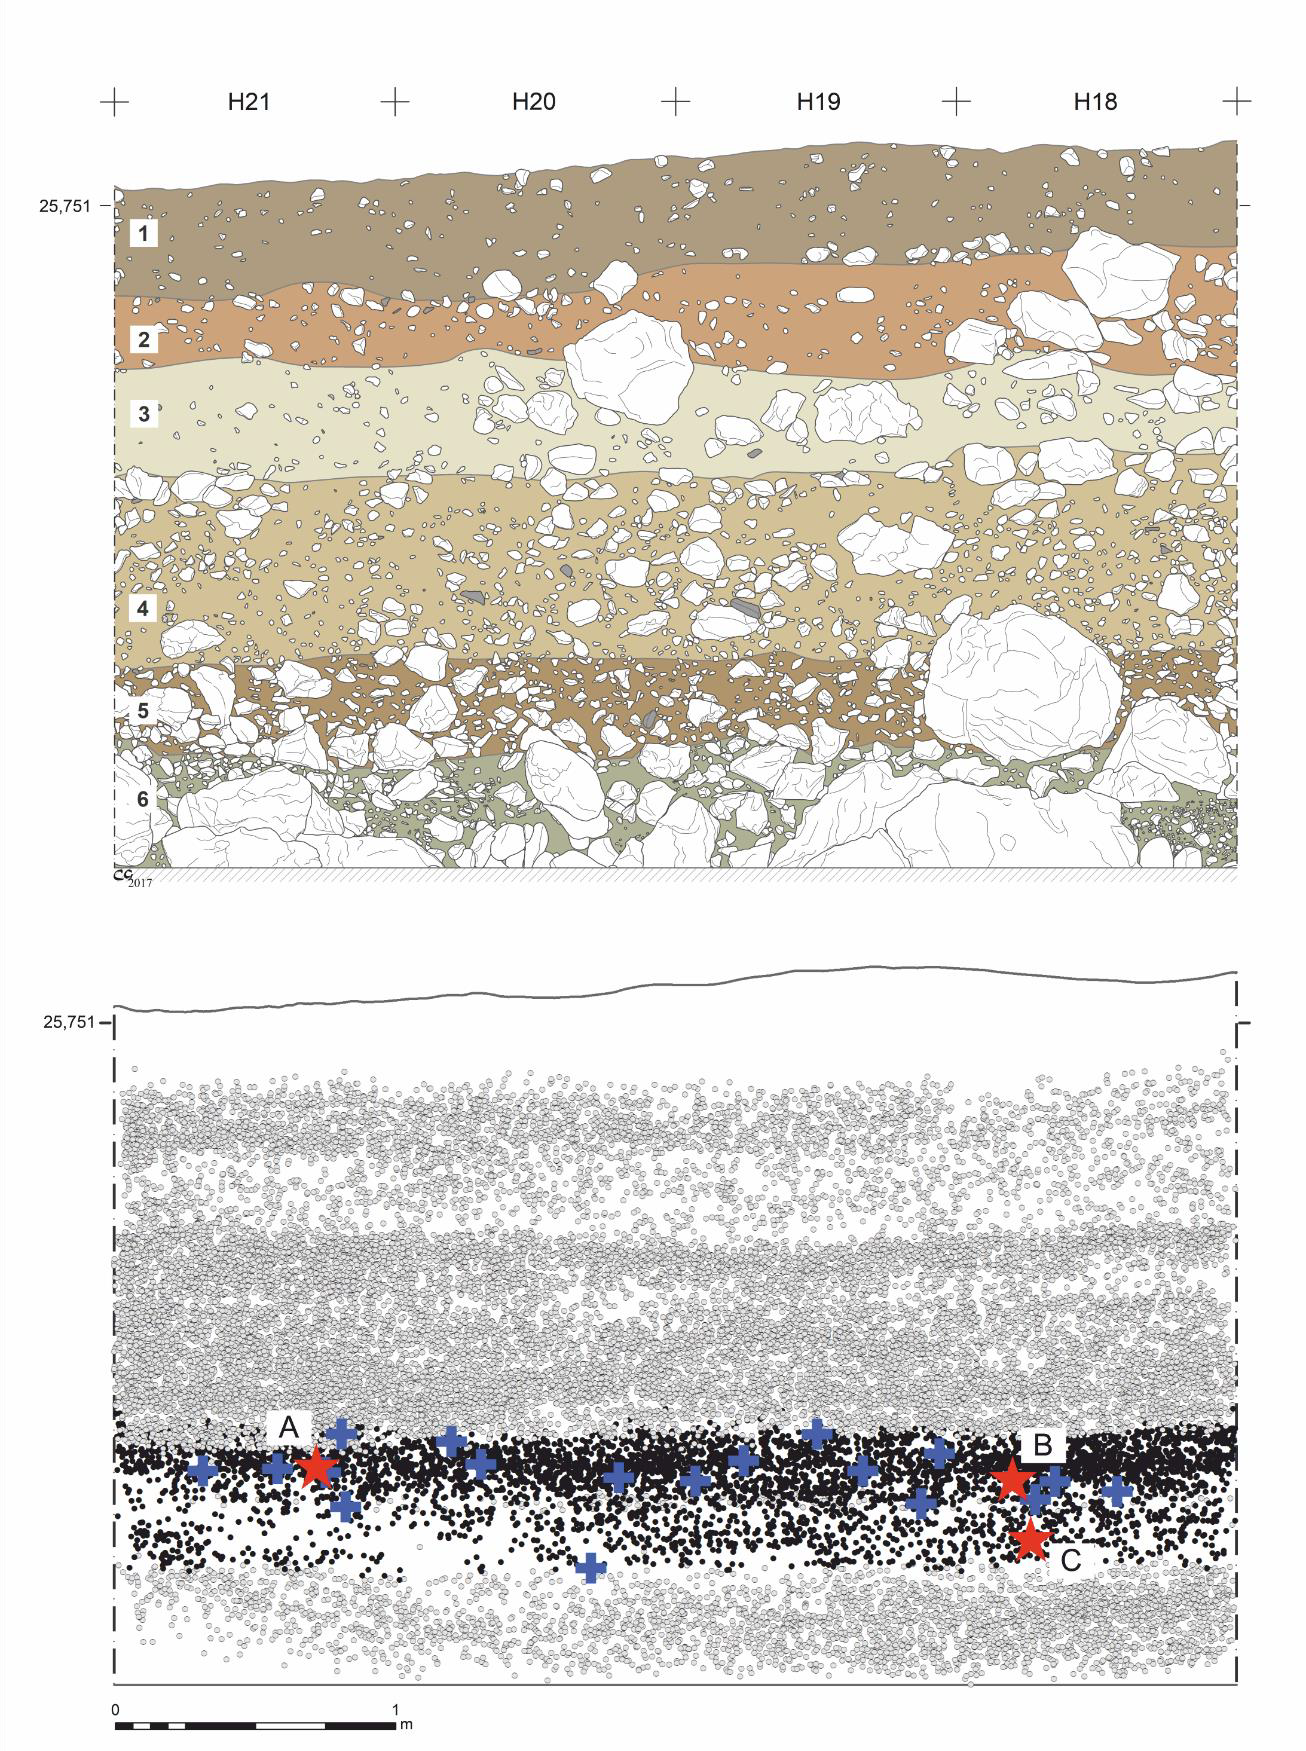
\includegraphics[width=1\linewidth]{figure/SpatialanalysisVB} \caption{East profile stratigraphy in the Terrace area (above) and distribution of all tridimensionally coordenated lithics in the new excavation area until 2017 (under). Lithis from layers 4E and 5 are coloured in black. Blue crosses represent dolerite artefacts and stars mark the provenance of each radiocarbon date: A - WK-42830; B - WK-42831; C - WK-44416.}\label{fig:spatialvbfig}
\end{figure}
\hypertarget{lapa-do-picareiro-1}{%
\section{Lapa do Picareiro}\label{lapa-do-picareiro-1}}

Lapa do Picareiro was first investigated during the 1950s by Marques, and then in 1964 by Fernandes Gomes and Gil Andrade, who excavated the cave and opened a test pit. Although the results have never been published, it is known the finds included several human remains associated with decorated pottery (Bicho 2000; Bicho 2006; Haws 2003; Zilhão 1997b).

Two decades after, in 1988, the site was revisited by João Zilhão and members of the STEA (Sociedade Torrejana de Espeleologia e Arqueologia). This visit resulted in the identification of several archaeological levels in the profiles from previous interventions, and the recovery of some archaeological finds that suggested the existence of an Upper Paleolithic context in the site (Haws 2003; Zilhão 1997b). One of these archaeological finds was a Vale Comprido point, found at the base of the test pit, by the cave wall (Zilhão 1997b). Despite the finds, these interventions did not include excavations.

The site was re-examined once again in 1994, by Nuno Bicho. This intervention confirmed the suspicion that the site was occupied during the Upper Paleolithic, with at least two occupations with deposits that seemed to extend deeper (Haws 2003).

From 1995 to 2001, the site was systematically excavated by Nuno Bicho and his team as part of an interdisciplinary project (Bicho 2000), which revealed 19 stratigraphic levels, 6 of which had archaeological occupations dated to the Magdalenian (Haws 2003).

These excavations were then resumed in 2005, under the direction of Jonathan Haws, which continue to the present day (Holst 2017), with 40 stratigraphic levels having been identified to a depth of 10 m (Benedetti et al.~2019), across which all the traditional Upper Paleolithic technocomplexes, as well as Middle Paleolithic levels, were identified.

Lapa do Picareiro shows a long sequence of occupations, from the Middle Palaeolithic, Upper Palaeolithic, Epipaleolithic, Neolithic and Bronze Age occupations, the latter mostly focused in the front of the cave, and adjacent outside areas (Benedetti et al.~2019; Bicho et al.~2006).

The Palaeolithic finds were, so far, recovered from two main areas: the main chamber and a niche in the rear wall. The main chamber shows a sequence of Middle to Upper Palaeolithic occupations, centered on units E7 to F8 (Benedetti et al.~2019). The main feature in this area is a large Magdalenian hearth in level F/G with associated lithics and a large quantity of fauna, which was interpreted as a particular purpose occupation for processing animal carcasses (Bicho et al.~2006). The niche finds, concentrated in units XX9 to ZZ11, present a series of smaller, stacked hearths, radiocarbon dated to the Magdalenian, Solutrean, Proto-Solutrean and Terminal Gravettian (Benedetti et al.~2019).

The large hearth and associated features are the only areas where human activity disturbed the sedimentary sequence. In all other areas, human activity is limited to thin hearths in association with sporadic lithic concentrations and modified bones. These periods of occupation appear in the sedimentary sequences as alternated with moments of faunal occupation, culturally sterile (Benedetti et al.~2019). Thus, human activity at the site might be understood as several occupations inside the cave throughout the late Middle and Upper Palaeolithic, which intensified through the latter with a significant peak during the Magdalenian.

(stratigraphy complete table)

Table X, adapted from Benedetti et. al (2019), shows the complete description of all currently identified levels in the site and, whenever existent, associated lithic assemblages. From the 34 levels described in the table, 23 show human occupations or association with a lithic assemblage, and 20 of these can be attributed to the Upper Paleolithic:

Magdalenian occupations are divided into Late Magdalenian (levels E-J) and Early Magdalenian (levels K-L). Late Magdalenian levels show a base brown color matrix and internal variability in terms of sediment, with variation between small to large clasts, and abundance of charcoal and bone fragments to few bones only. Early Magdalenian levels show less variability, presenting a dark brown color matrix, and friable sediment with small to medium clasts and few bones.

Solutrean occupations occur in levels O, R, and S (level P showing neither bone fragments nor a lithic assemblage), maintaining a brown color matrix but varying between dark to light. The sediment is friable, composed of small to medium clasts, with the frequent presence of charcoals and bones.

Level T, approximately 50 cm thick, has a dark brown color matrix, with the presence of medium to large clasts and boulders, and abundant charcoal and bones. The sediment is reddish and muddy in the lower half. This level is comprised of several lithic assemblages: Solutrean in the upper level; Proto-Solutrean in the middle portion of T; and Terminal Gravettian in the lower portion of the level (Benedetti et al.~2019).

The Terminal Gravettian occupation was also identified in level U, a \textasciitilde15cm thick layer with a brown color matrix and, near the rear wall, a reddish muddy matrix that resembles lower T sediment. It has small to medium clasts and includes several lenses with abundant small animal bones and bone fragments.

Levels V, W, and X were associated with Gravettian occupations, all three showing a dark brown matrix, with variation between muddy and fine sediment, all with the abundant presence of small animal bones.
Levels BB, DD, and FF (each intercalated with a culturally sterile level), varying between a dark brown and reddish-brown color matrix, have an associated Early Upper Paleolithic lithic assemblage, with internal sediment variability but the frequent presence of bone fragments and small to medium clasts.

An Aurignacian occupation is present in level GG, which presents a dark brown color matrix, and a slightly hard to very hard sediment matrix, with the presence of calcite cement, bones, and bone fragments.

The stratigraphic sequence, as mentioned before, shows an alternation between faunal occupations, rich in bones and bone fragments, and clearly defined cultural horizons, which is explained by the continuous long-term accumulation of sediments, a result of the cave setting and cave morphology. These factors not only allowed continuous deposition but also contributed to the preservation of fauna and lithics. The sequence also shows good stratigraphic integrity, without the presence of bioturbation in its interior (signs of bioturbation by the action of roots are only present at the entrance of the cave) (Benedetti et al.~2019).

\hypertarget{levels-u-and-lower-t}{%
\section{Levels U and lower T}\label{levels-u-and-lower-t}}

The physical distinction between level U and the lower portion of T is hard to make near the niche. In this area, both levels show similar reddish muddy sediment and the presence of animal bones in level T increases. As such, in this area, the attributed level to the recovered artifacts was T/U instead.

Layer T/U is about 15 cm thick, with the presence of possible combustion features and distinct activity areas. The recovered artifacts show a rich faunal assemblage, with a high presence of red deer, though ibex presence is also important, and a superabundance of rabbit bones. A few bone tools were also found. Other recovered artifacts also include a perforated marine shell and a perforated red deer canine tooth.
\begin{figure}
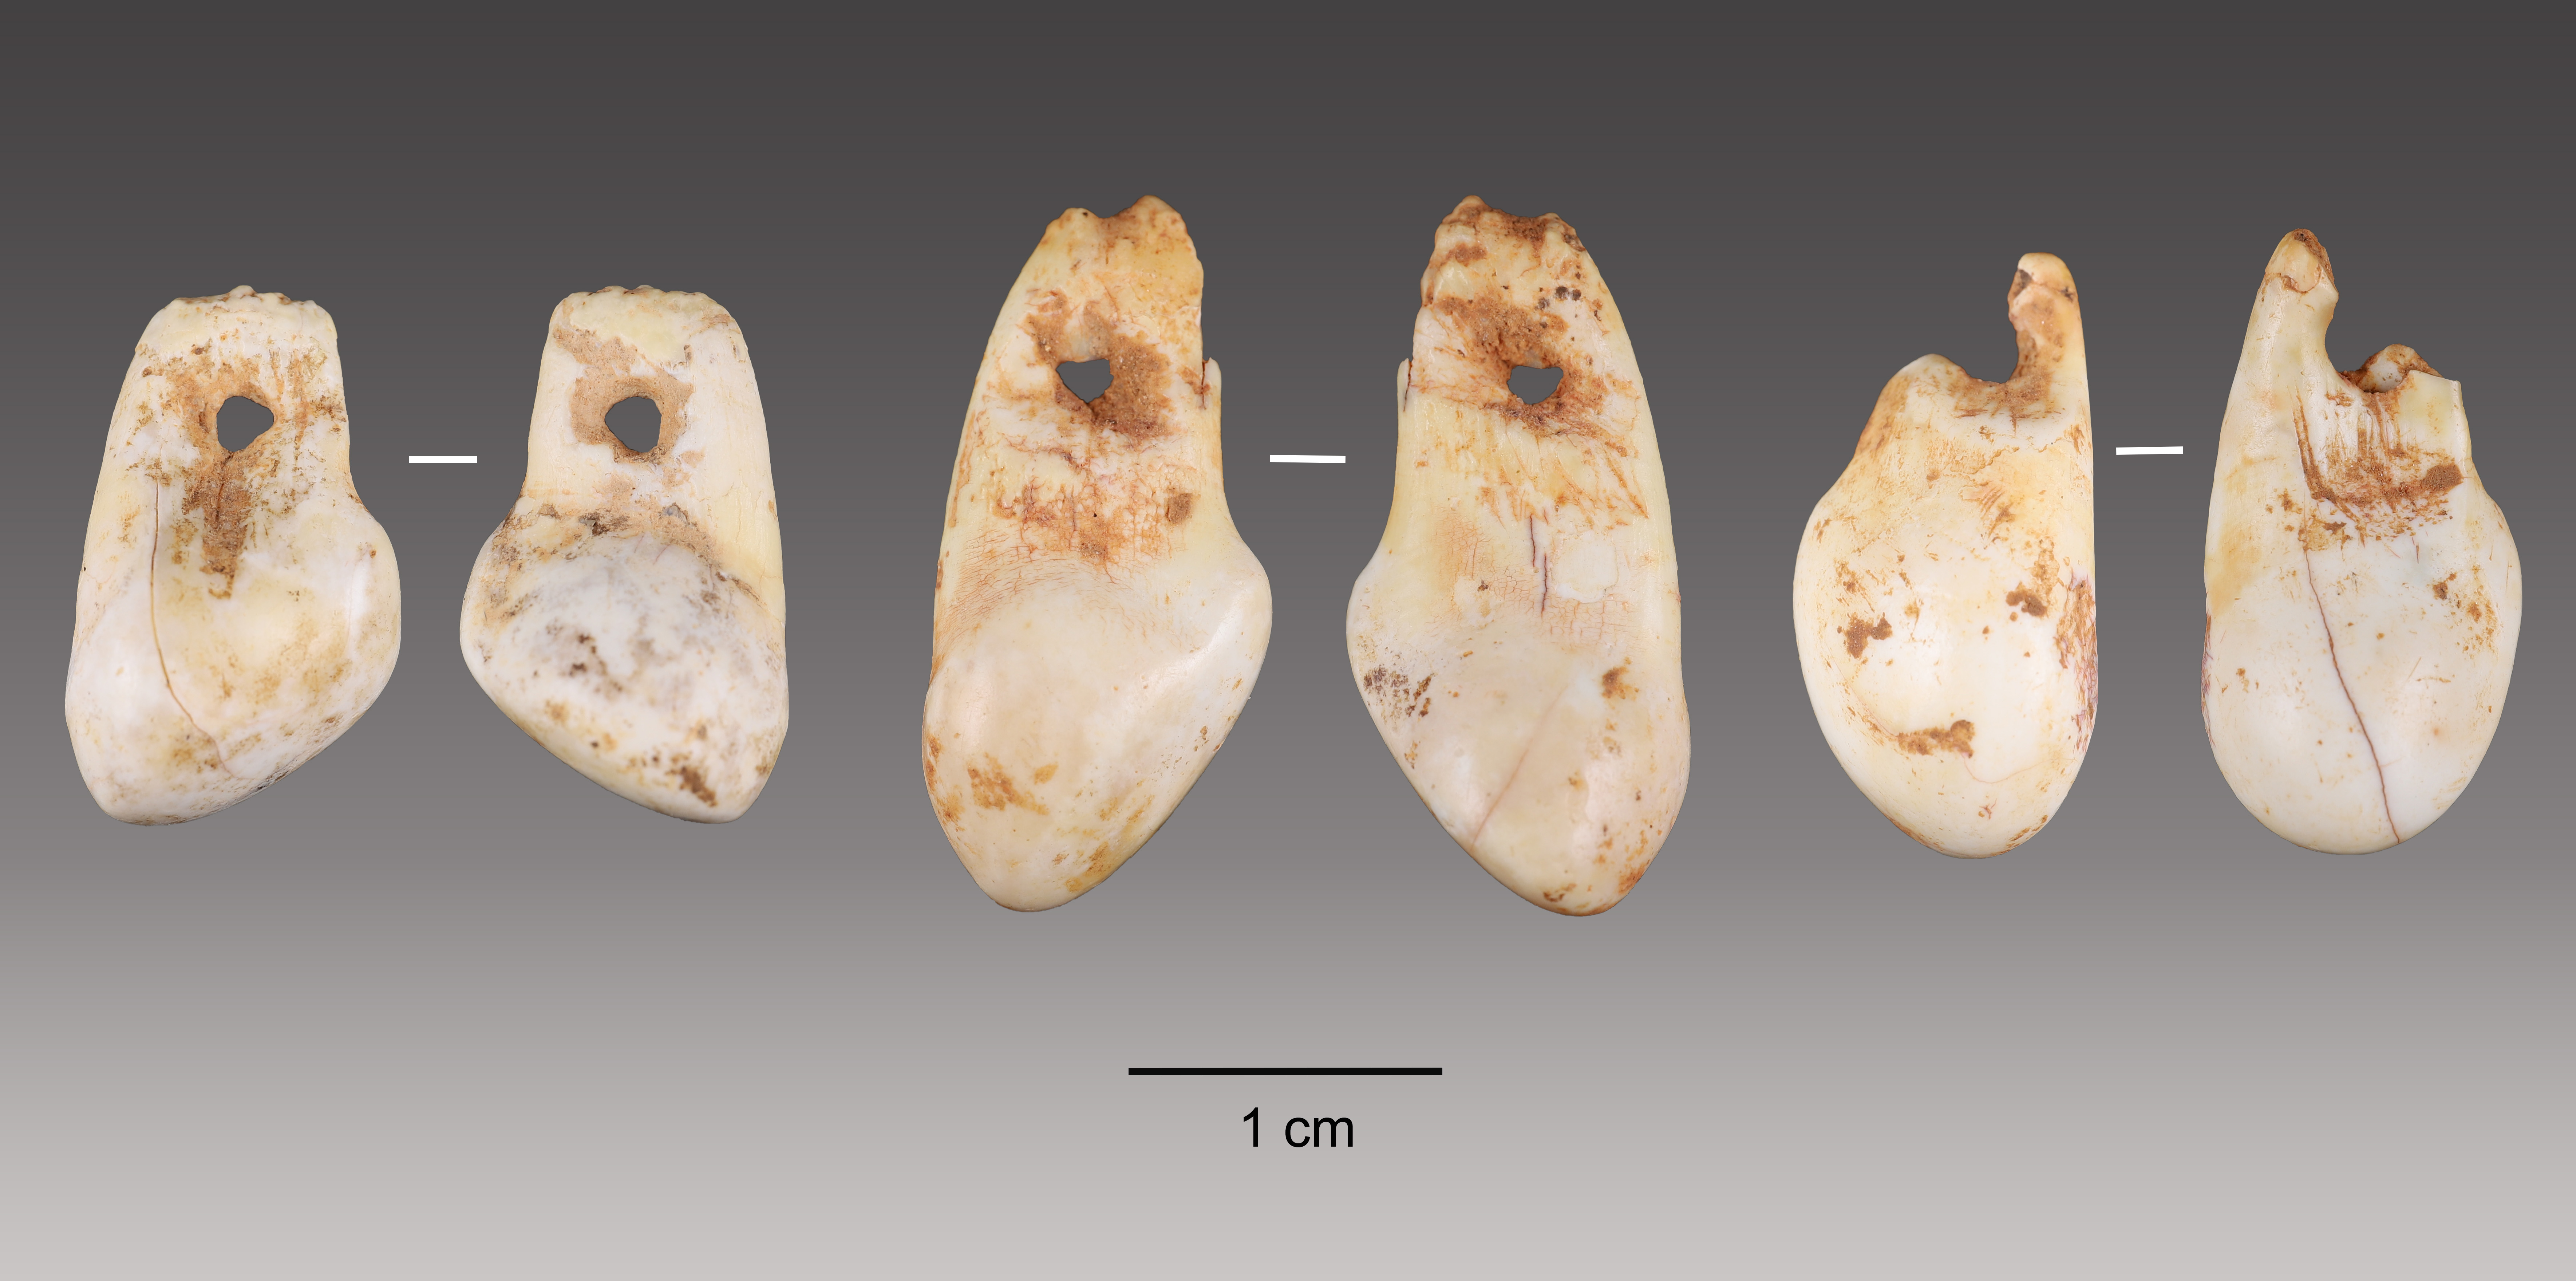
\includegraphics[width=1\linewidth]{figure/LP_teeth} \caption{Level U and lower T perforated red deer canine teeth. After Haws et al. 2019.}\label{fig:unnamed-chunk-6}
\end{figure}
\begin{figure}
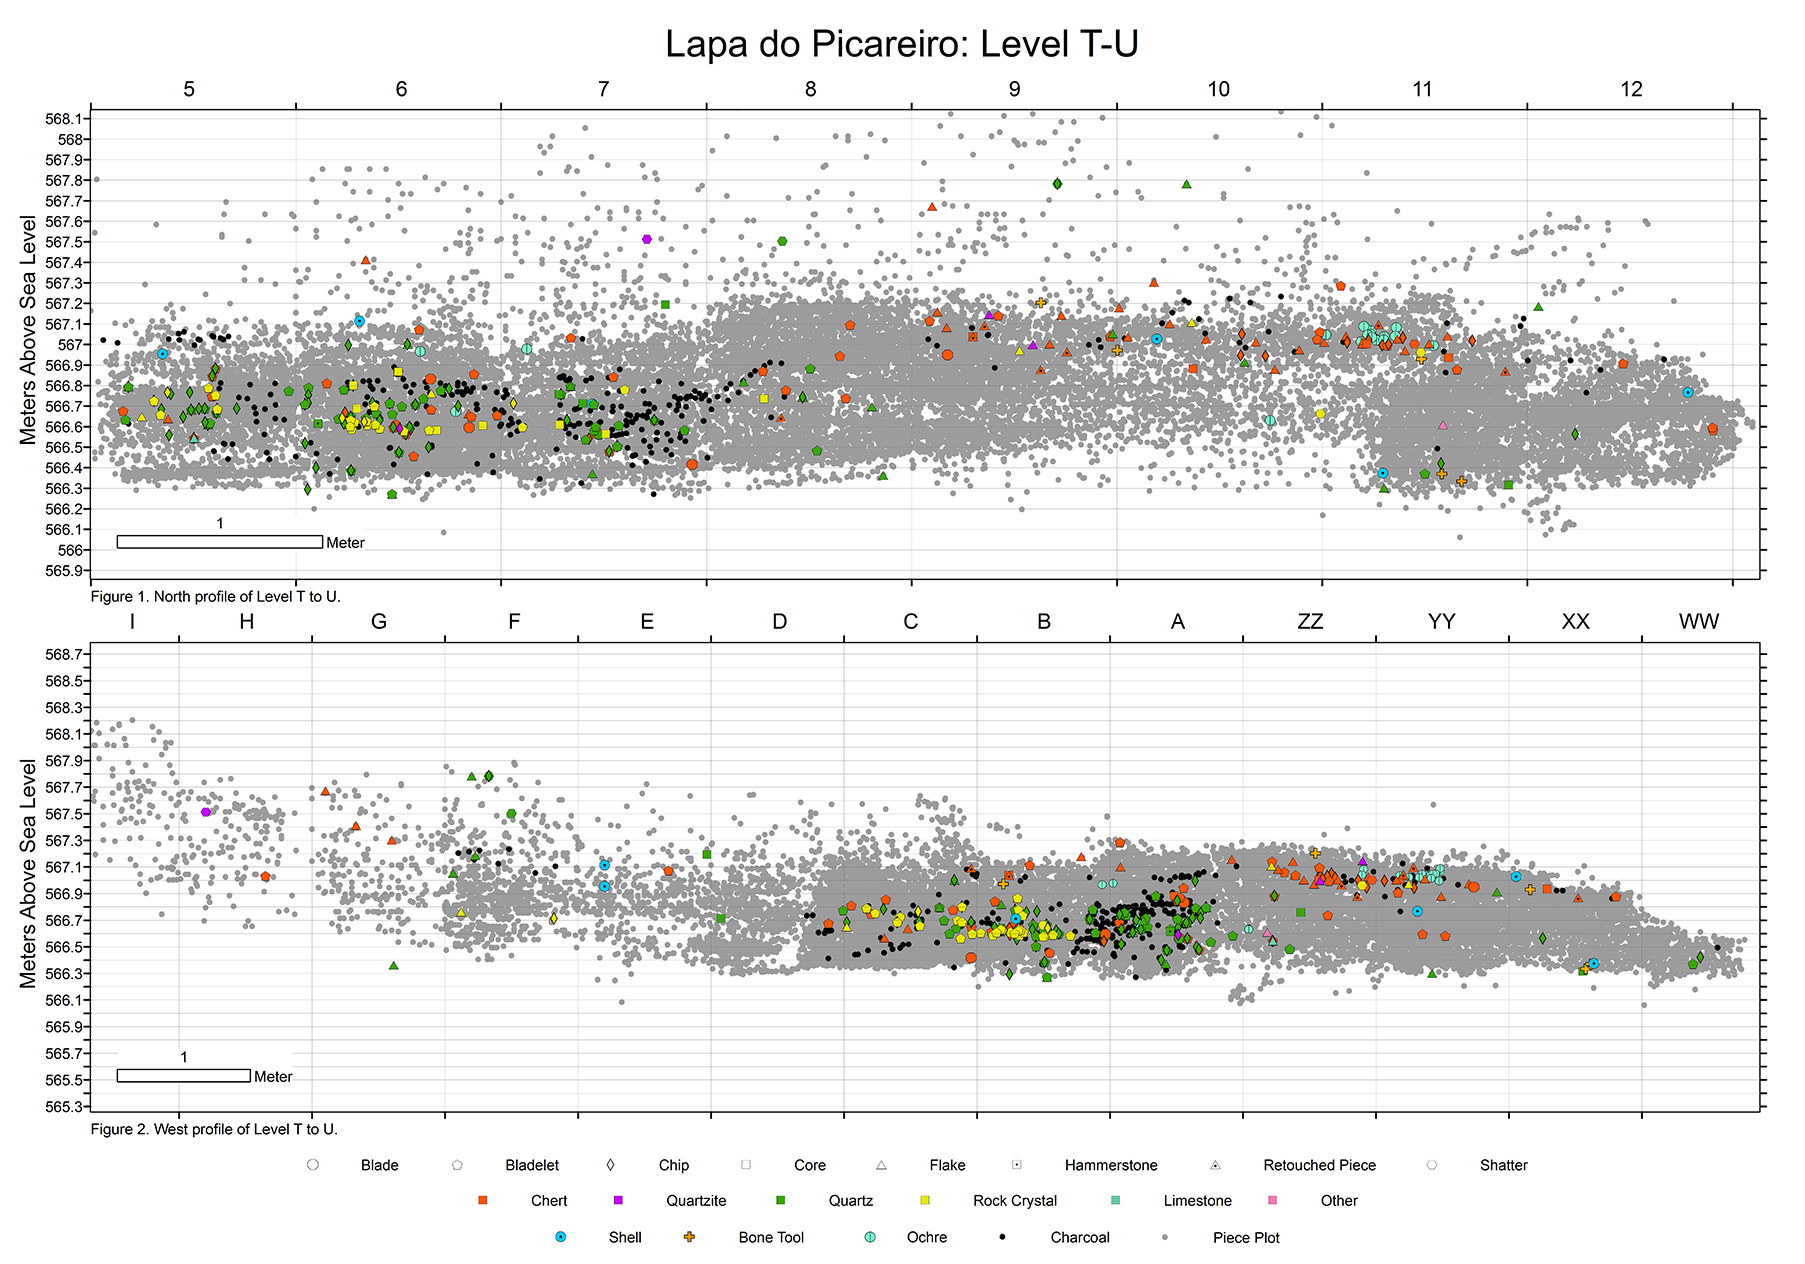
\includegraphics[width=1\linewidth]{figure/LPspatial} \caption{Spatial distribution of all plotted artefacts from levels T-U (in grey), lithic artefacts in colours and shapes refering to raw material and class. After Haws et al. 2019.}\label{fig:unnamed-chunk-7}
\end{figure}
The niche area was where most of the lithic assemblage from these levels was found. As shown in image X, there is an apparent concentration of lithics, comprised mostly of quartz and rock crystal, and some chert, all raw materials appearing mostly in the shape of bladelets.

For U and lower T, the dates (table), all obtained from charcoal samples, show results of c.~27-26 cal ka BP, except for one of lower T dates which presents a result of c.~25-24 cal ka BP.

(T and U dates table)

The middle part of T shows the presence of circular concentrations of charcoals, about 10-15 cm thick, which have been interpreted as hearths. Aside from these features, there is a high frequency of animal bones, following the same species patterns as level U and lower T (although these results are preliminary).

The lithic assemblage in this portion of level T is found in two areas: an accumulation of lithics surrounding the hearths and other scattered pieces in the same spits as the hearths but in different units. This assemblage is mostly comprised of chert, with the presence of quartz and rock crystal, in the form of bladelets and flakes. Although the presence of traditionally-defined Vale Comprido points is not completely attested, there are several blanks which seem to resemble this type of technology, in the form of convergent elongated blanks.

The dates for middle T (table), obtained from charcoal and bone samples, provided results of c.~25-24 kcal BP, with one date presenting a range of c.~23.4-23.6 kcal BP.

There is a clear separation between the two groups, one composed level U and lower T, and the other of middle T. This is particularly evident on the spatial dispersion of lithics and other artifacts shown on figure X, where there is an accumulation on the bottom left, correspondent to the U/T levels, and another aggregation in the middle portion, to the right, ranging from 20-40 cm of depth difference between the groups.

The patterns in the lithic assemblages also indicate a clear difference between the groups: the high frequency of quartz/rock crystal bladelets of U/T shows a marked difference from the middle T, where chert frequencies are higher, and there is a more balanced frequency of bladelets and flakes. In this case, the U/T assemblages shows patterns which can be attributed to the Terminal Gravettian (Almeida 2000; Benedetti et al.~2019), the intermediate phase described by the three-stage model for the Proto-Solutrean, while the middle T assemblage shows patterns best explained by the Proto-Solutrean phases of the model (Zilhão 1997a).

Finally, the dates for both U/T and middle T strengthen further the separation between the occupations, showing a gap of c.~2 k years between the assemblages, and placing the Terminal Gravettian occupation somewhere around 27-26 cal ka BP and the Proto-Solutrean occupation at c.~25-24 cal ka BP, with at least dates widening this range to c.~23 cal ka BP.

These clear spatial, raw-material and chronological differences, while maintaining some technological similarities, are consistent with the three-phase model developed for the evolution of the Proto-Solutrean in the Estremadura, where there are two distinct moments with chronological relevance which cannot be better explained by the existence of a functional facies.

However, the dates are not in concordance with the models developed for the Proto-Solutrean in the Portuguese Estremadura (Zilhão 1997). The lower depth group, which has been determined as Terminal Gravettian, shows concordance with dates for other sites (e.g.~Lagar Velho) placing these occupation in the transition between the Final Gravettian/Terminal Gravettian. The dates associated with the highest quantity of chert, however, seem to extend the Proto-Solutrean chronological range to much younger dates (leaving out WK-37655c and UGAMS-23727, which show signifcant chronological differences from the other dates), placing it at the 24 ka cal BP, similarly to Vale Boi.

\hypertarget{excavation-methodology}{%
\chapter{Excavation methodology}\label{excavation-methodology}}

Both sites are mapped using a 1x1 m alphanumeric grid system, creating a combination of lettered and numbered rows, which correspond to the excavation units. The deposits were excavated by natural litho-stratigraphic units, subdivided into 5 and 10 cm spits for Vale Boi and Lapa do Picareiro, respectively.

Within each spit, the 3D location of all artifacts with dimensions superior to 2 cm is recorded with a Total Station, except for small complete artifacts, such as ornaments, complete bones or small bladelets, which are always recorded despite their size.

All pieces have a sequential Identification Number (ID) by unit. This ID is given by the software EDM where all the contextual information of the artifact is recorded (layer, spit, unit, and code), which is then associated with the materials through pre-printed labels. Each label has an ID, site designation and a barcode which allows accessing artifact information in the lab. The same type of label is used for the materials recovered from the sieves that correspond to all materials found in each 10 L bucket of sediment for Vale Boi and each artificial spit for Lapa do Picareiro. In Vale Boi the association with Total Station data is made by measuring a coordinate in the center of the excavated area from where the sediment is coming from. All sediment is sieved using 3 mm mesh grids in the case of Vale Boi. At Lapa do Picareiro sieves with 2 mm and 4 mm meshes are used. The latter is sorted in the field, while the smaller sieve sediment is taken to the laboratory for water screening, in order to recover small bones or other types of artifacts like lithic chips.
\begin{figure}
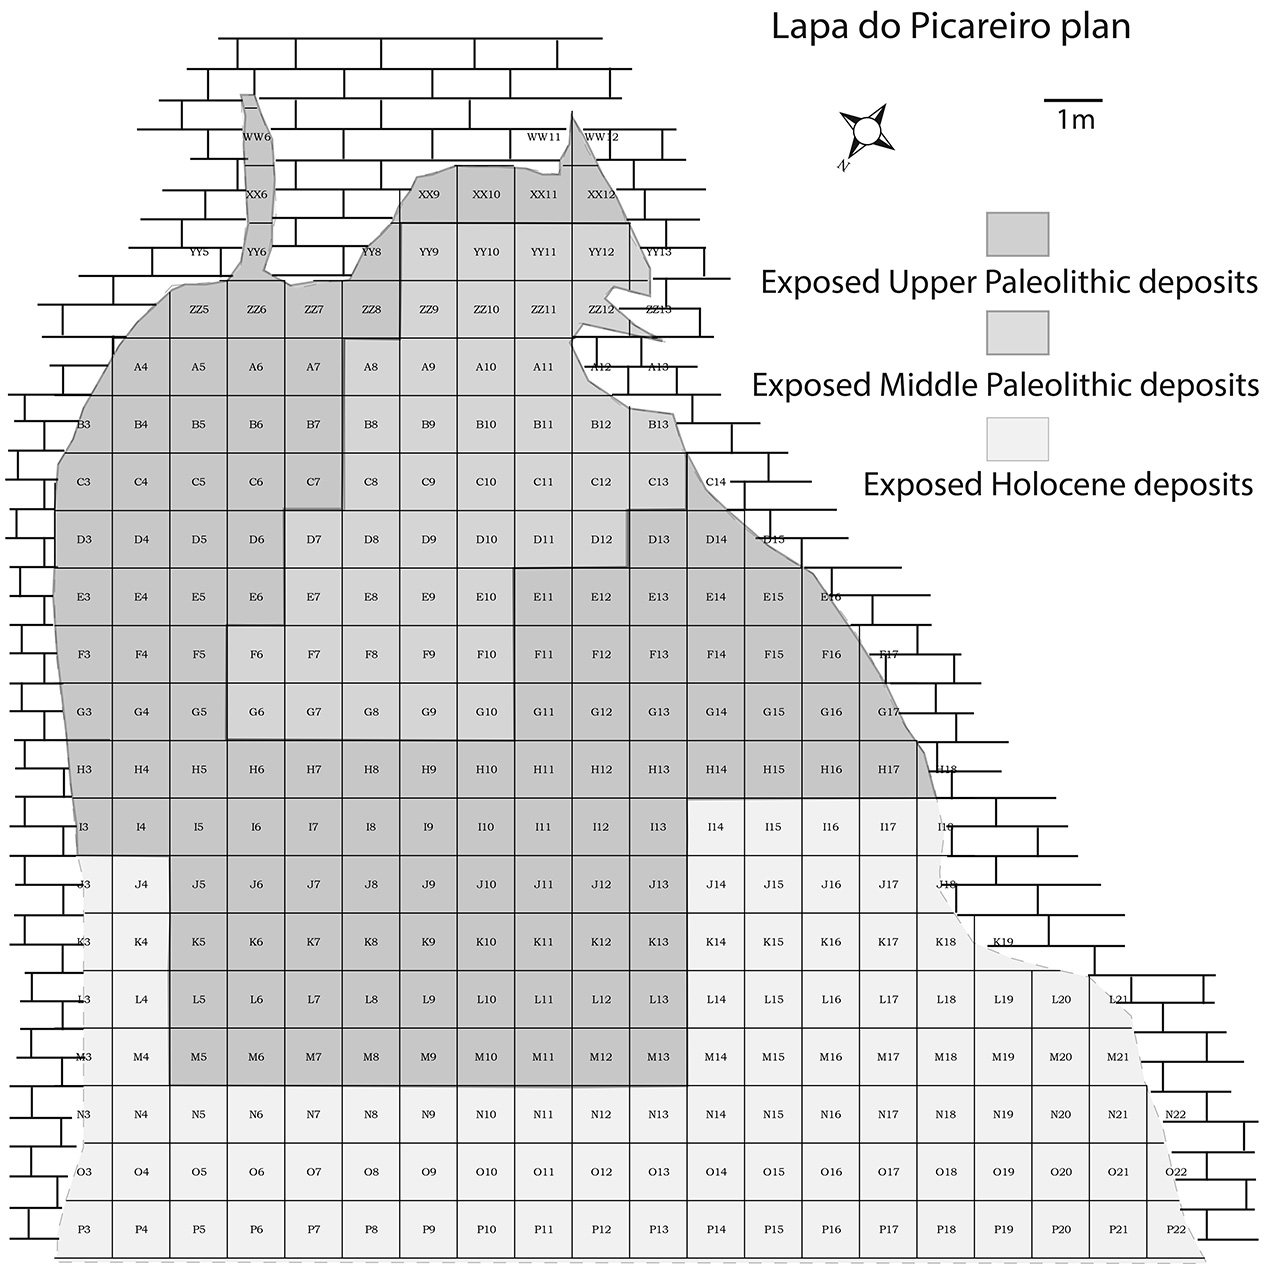
\includegraphics[width=1\linewidth]{figure/LP_units} \caption{Lapa do Picareiro unit plan grid.}\label{fig:unnamed-chunk-8}
\end{figure}
\hypertarget{methodology}{%
\chapter{Methodology}\label{methodology}}

\hypertarget{attribute-analysis}{%
\section{Attribute analysis}\label{attribute-analysis}}

In order to understand the multiple causes for lithic variation, such as raw material properties or local adaptations, researchers are increasingly adopting sophisticated methods of lithic analysis, then linking that data to explanatory theories of human behavior (Scerri, Groucutt, Jennings, \& Petraglia, 2014). Examples of such studies are those by Brantingham \& Kuhn (2001), who apply a geometric and mathematical model to understand Levallois core morphology, or Dibble \& Rezek (2009), that through platform attributes try to understand flake variability.

Despite the existence of several different concepts in quantitative analysis, the basic units of analysis continue to be the technological attributes (Scerri et al., 2014). These attributes are measurable (e.g.~length, width or thickness) and observable (e.g.~platform type or cross section type) proxies for understanding lithic shape and production methods (Inizan, Reduron-Ballinger, Roche, \& Tixier, 1999). Following certain paradigms, like referred above, they can be quantified in different ways, such as diversity, mechanical relationships, shapes and reduction sequences, in order to better understand lithic assemblages (Scerri et al., 2014) and the role that lithics played in past adaptations over time and space (Foley \& Lahr, 2003).

Despite the caveats in the application of attribute analysis, linked mainly to how such attributes are interpreted by the archaeologist and their actual contribution to the understanding of an assemblage's variability (Dibble, 2008; Scerri et al., 2014), this approach was chosen for the present study, for the recognized benefits such as flexibility (resolution and amount of information recovered) and broadness of utility (Tostevin, 2012).

The application of this methodology, which aims to recover morphological and metrical attributes of technological classes, has been present in pre-historical European contexts since the 1970s (Bicho, 1992). In Portugal, this methodology has been applied by Bicho (1992) who characterized Rio Maior's Upper Paleolithic lithic assemblages, Zilhão (1997) for the Upper Paleolithic archaeological sites of Estremadura or Almeida (2000), who associated attribute analysis with refitting to characterize the Terminal Gravettian of the Estremadura.

Regarding the latter approach, refitting, despite allowing a precise description of the sequences of knapping operations from the beginning of the knapping sequence to the final desired products, have too many caveats for its application in the present study (Tostevin, 2012). Often, assemblages may not gather the requisites which are necessary for the application of this methodology such as adequate contextual preservation or presence of complete in situ knapping sequences, or the investigators may not have either the time or space for it. Additionally, one or two totally refitted nodules may or may not be representative of the dominant operative sequence, especially in situations where there is high internal variability (Tostevin, 2012). As such , and because the Vale Boi assemblage shows a high degree of variability, and Lapa do Picareiro's assemblage shows a truncated assemblage (due to site function and high altitude location), the present study used only an attribute analysis approach without refits.

All artefacts and their technological and morphological attributes were recorded using two different databases, thus dividing the analysis in two phases: basic and complete attribute-based analysis .
In both cases, data collection was done through E4, a software developed by Dibble and McPherron (2003), available for download at \url{http://www.oldstoneage.com/software/default.shtml}. The software allows the user to program a database file which filters variables through conditions, defined by previous choices and attributes, which allows for better control of the database and homogeneous results. After recording, all information is gathered in one single database in an Access type output.
The basic analysis (appendix X) was applied to all of Vale Boi's quartz artefacts (layers 5 and 4E), since all lithics from the same assemblage in other raw-materials (e.g.~chert and greywacke) had been previously analyzed with the same database (\emph{vide}, Belmiro, 2018). This database consists of a reduced set of variables which allow for the general classification of metric and morphologic characteristics of the artefacts, as well as the identification of raw material preference and preferential use. These main variables were: 1) raw material; 2) technological class, following the traditional criteria for lithic technological analysis (Andrefsky \& Andrefsky Jr, 1998; Bicho \& Jorge, 2011; Debénath \& Dibble, 1994; Inizan et al., 1999); percentage of cortex (Bicho \& Jorge, 2011); weight and mesial thickness, maximum width and maximum length. Retouched pieces were classified into large groups regarding their morphologies and retouch type, following the typologies defined by Sonneville-Bordes \& Perrot (1956), adapted by Zilhão (1997) for the Portuguese Estremadura.

The complex analysis was applied to Vale Boi complete cores, debitage products and retouched pieces. Only pieces which were complete were chosen for this stage for two main reasons: 1) the collection is well preserved, with high percentages of complete cores and blanks (\textasciitilde80\%), guaranteeing that the sample is representative; 2) only complete pieces gather all the necessary attributes and data to apply the multivariate analysis approach used here. The same database was applied to the whole assemblage of Lapa do Picareiro, given its small sample size.

The several attributes analysed in this database follow those present in specialized literature, such as Brézillon (1968) and Tixier \& Inizian (1980), paired with the methodologies used in Upper Paleolithic lithic attribute analysis works, such as Bicho (1992), Zilhão (1997) or Almeida (2000).

The complete Data Dictionary with all variables, attributes, values and description, with reference to the consulted literature can be found in Appendix X.

Regarding cores, the following variables were registered: section, type of platform and number of platforms, core morphology, following the types defined by Bicho (1992) and Brézillon (1968), percentage of cortex, types and number of extracted products (with maximum, proximal, mesial and distal measurements of the final extraction) and reason for abandonment. When cores showed more than one face, a dominant debitage face was established, which allowed for the orientation of the artefact and recording of some of the variables (e.g.~measurements of final extraction).

For debitage products and EMNP it was recorded their technological class, morphology, section and profile, following the definitions by Zilhão (1997). It was also identified the presence of lipping and type of platform, according to Inizan et al. (1999), percentage of cortex and amount of dorsal extractions (\textgreater{} 5 mm). Retouched pieces were classified into large groups as applied in the simple database, following once again the typologies defined by Sonneville-Bordes \& Perrot (1956), adapted by Zilhão (1997) for the Portuguese Estremadura.

Regarding the technological classes, the values recorded were core, blank, retouched piece, core preparation product and bifacial thinning flake following traditional analysis criteria (Andrefsky \& Andrefsky Jr, 1998; Bicho \& Jorge, 2011; Debénath \& Dibble, 1994; Inizan et al., 1999), but collapsing both flakes and elongated blanks in a single category. The difference between flake and elongated blank is traditionally defined by a ratio between length and width measurements. Elongated blanks are defined as products whose length is equal or greater than twice their width (Bicho \& Jorge, 2011; Tixier \& Inizian, 1980). Very frequently, this ratio is blurred, resulting in elongated flakes or short elongated blanks, which may result in incorrect classifications. In understanding both flakes and elongated blanks as a whole, without prior classification, and using the measurements recorded if needed, we achieve the same results without the need to find classification mistakes and without delving into typologies which may not have any real technological significance. The same methodology was applied regarding the definition of bladelet and blade. As traditionally defined, bladelets are elongated blanks with maximum width of 12 mm, whereas blades are elongated blanks with more than 12 mm of width or more than 50 mm of length (Tixier, 1963). For the present study, this typological differentiation was not applied during the analysis, since it may be achieved, if needed, with the recorded measurements.

The measurements were registered equally for debitage products and cores as shown in image X, which included the measurement of the platform angle according to Dibble (1997), with the goal of understanding platform morphology, which, according to the author, may offer a better understanding of lithic technological variability. In this case, the variation in exterior platform angle, platform depth and angle of blow seem to explain flake size, and the variation of the exterior platform angle seems to have an impact on flake shape as well, both of which have implications in understanding the employment of different strategies for preferential size of blank products (Dibble, 1997; Dibble \& Rezek, 2009; Leader, Abdolahzadeh, Lin, \& Dibble, 2017; Lin, Rezek, Braun, \& Dibble, 2013).
\begin{figure}
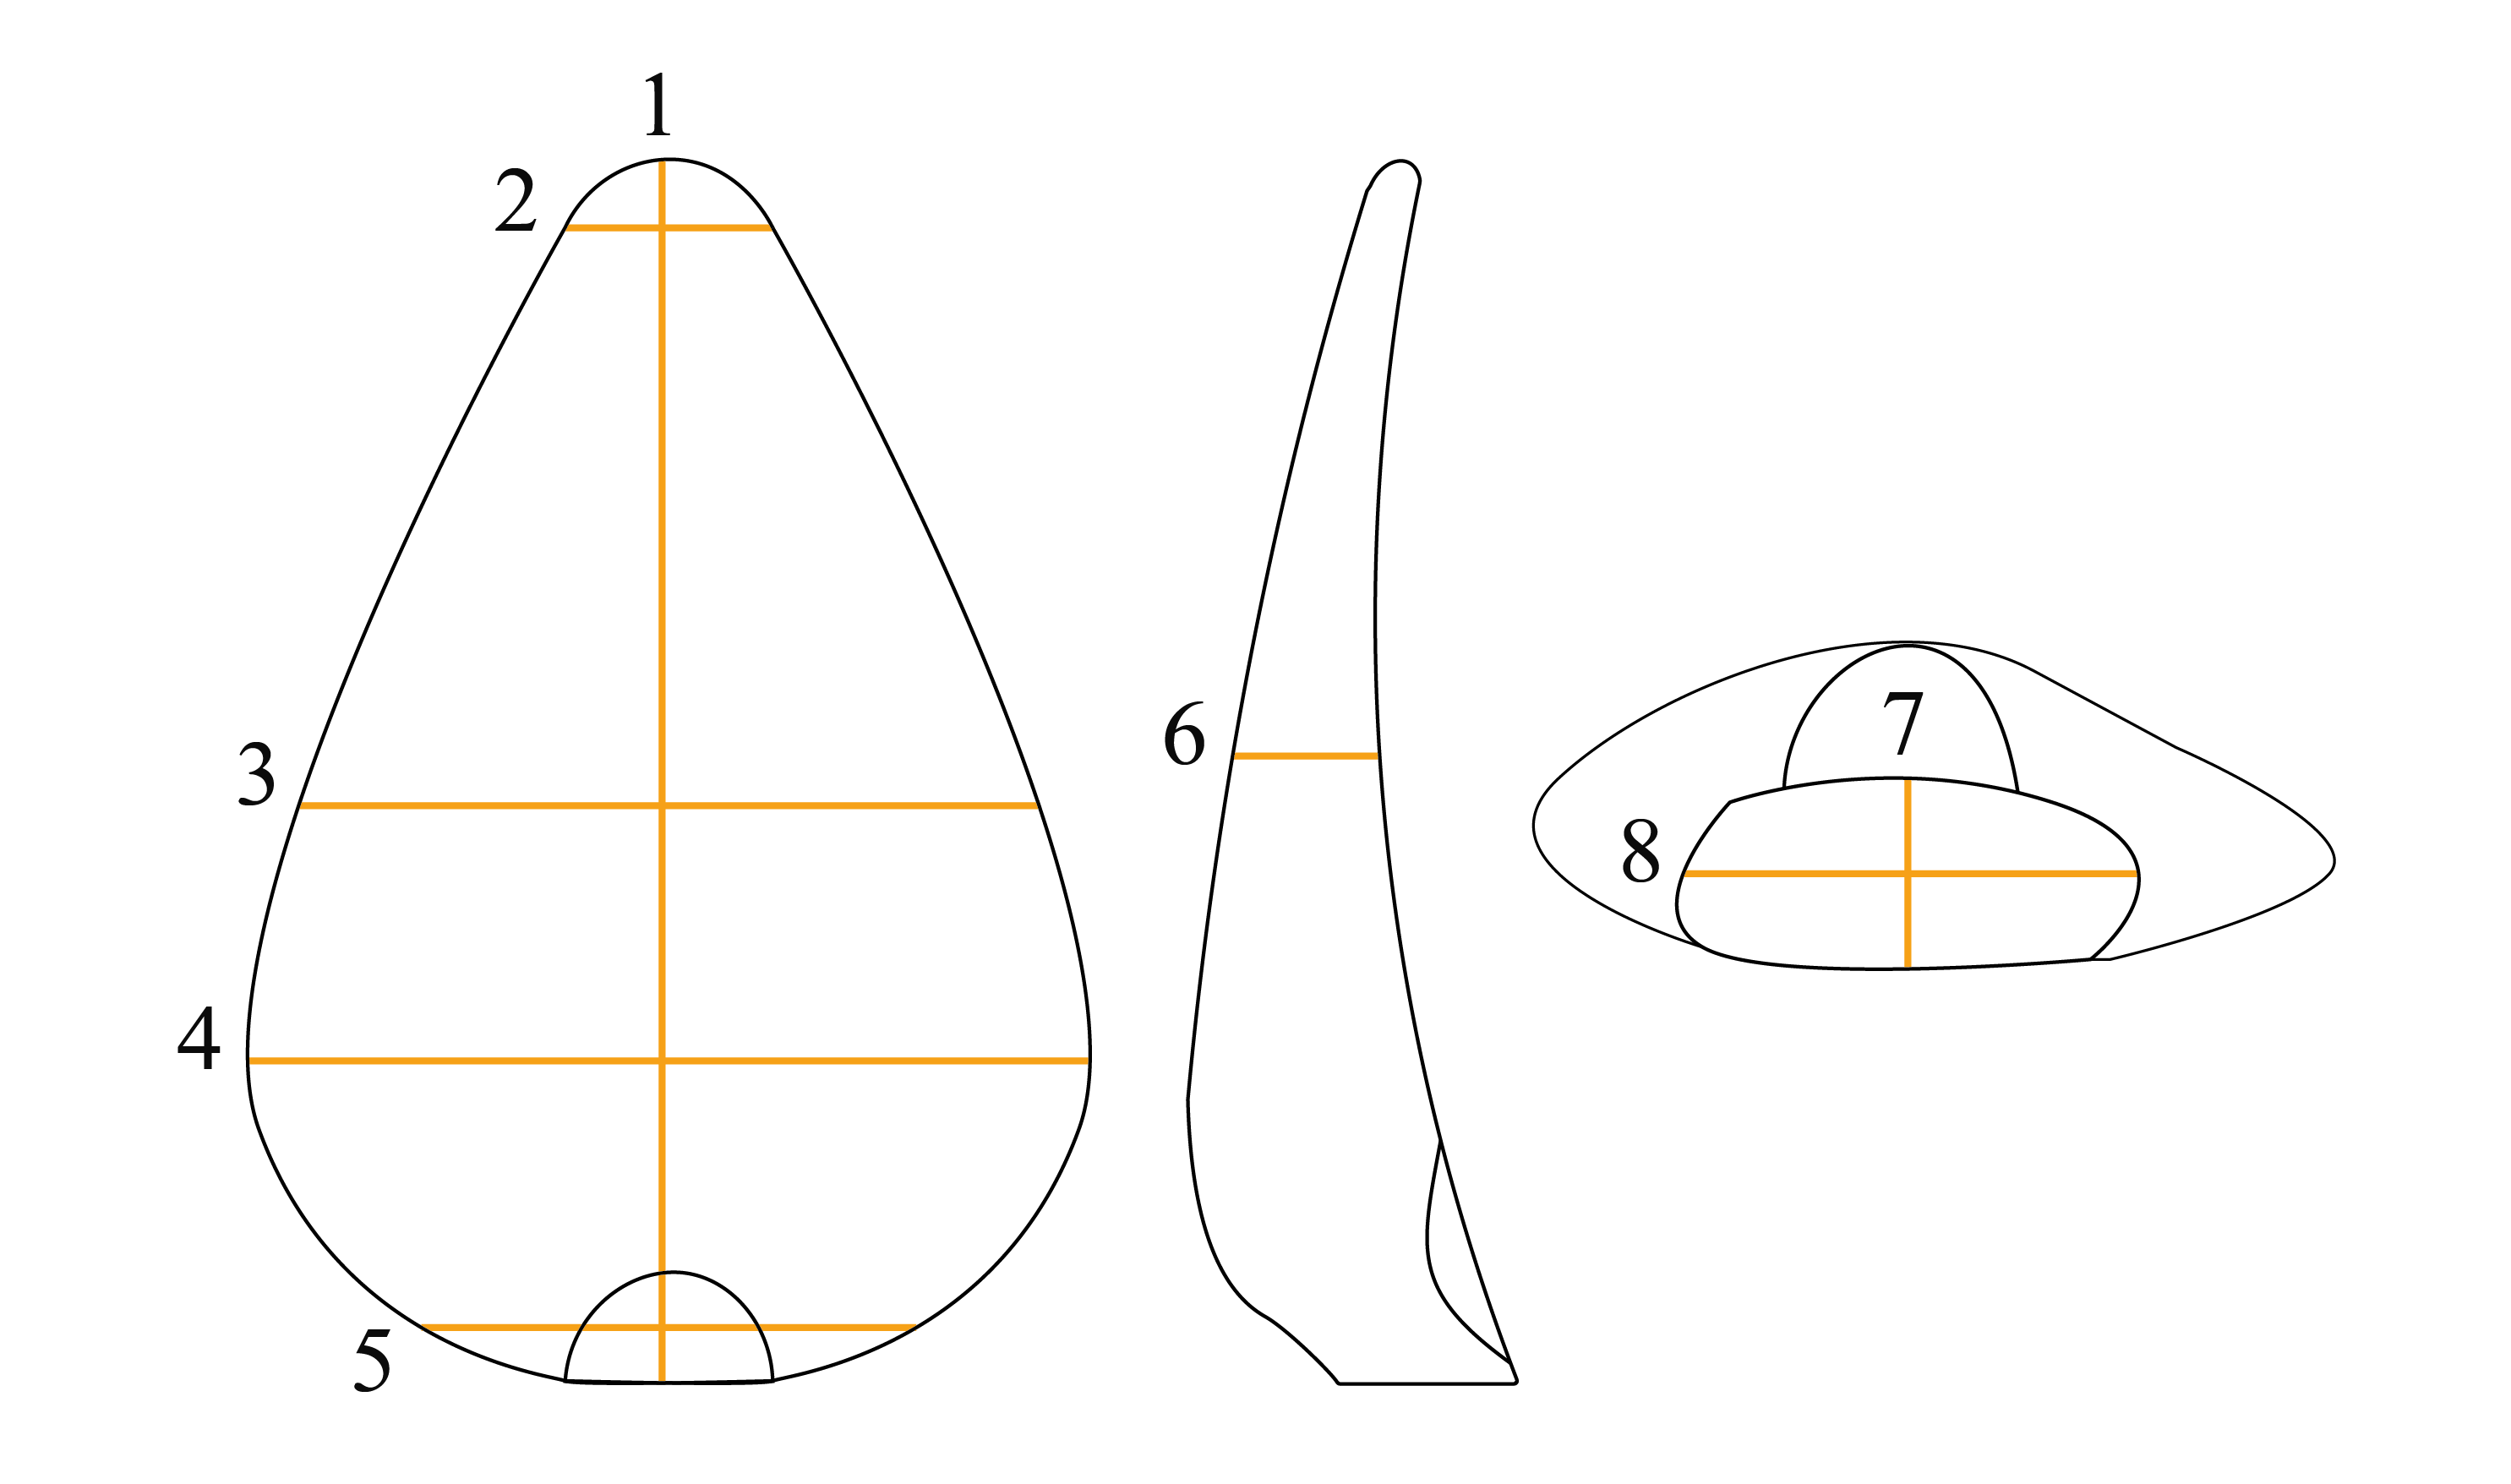
\includegraphics[width=1\linewidth]{figure/Metrics-01} \caption{Registered measurements scheme for debitage products and cores. Legend: 1- Maximum length; 2- Distal width; 3- Mesial width; 4- Maximum width; 5- Proximal width; 6- Mesial thickness; 7- Platform thickness; 8- Platform width.}\label{fig:unnamed-chunk-9}
\end{figure}
Finally, although raw material had been previously analysed in the simple attribute analysis, quartz artefacts were subdivided regarding raw material quality. When analysing the quartz lithic collection, it was apparent that fracture patterns and product morphology differed greatly between quartz and other raw materials and even within types of quartz. In fact, it is understood that applying the same analysis variables to all raw materials, especially quartz, may not be the most appropriate methodology, since different technological solutions might be applied to materials which react differently to knapping (Beardsell, 2013). Despite this, creating a different database or establishing different analysis attributes for quartz would result in different issues and problems that would require further testing and experimenting. Thus, in order to understand possible preferential uses or mechanical constraints of quartz, this raw material was analysed with the same attributes as other raw materials, but further classified regarding its quality. In fact, Almeida (2000) stated that, for the Terminal Gravettian, raw material quality, namely the quartz, resulted in specific behaviours and different technological patterns. By defining quartz quality and understanding the collection through this added variable, it was our goal to better comprehend the cultural horizon in its fullest, and allow comparison to other studies, in which similar variables were considered.

Quartz quality was defined by grain size: coarse quality was applied to every quartz artefact that displayed large and visible grains (\textgreater0.5 mm); medium quality was applied whenever the grains were visible but small; fine quality was defined by the absence of visible grains; and rock crystal was applied whenever there was the absence of visible grains, but where the minerals were completely transparent.

\hypertarget{data-analysis}{%
\section{Data analysis}\label{data-analysis}}

After data collection, the databases, for both Vale Boi and Lapa do Picareiro were imported into R environment, where the information was processed through the creation of descriptive and multivariate statistical analysis. This and the writing of this thesis were done in RStudio, an open source integrated development environment (IDE) for R, which can be downloaded at \url{https://rstudio.com} , also with resource to RMarkdown, which allows the production of fully reproducible documents (downloaded at \url{https://rmarkdown.rstudio.com}) Following the goal for transparent science and reproducible results, the script programmed for this analysis as well as all the raw data used can be consulted online through the following DOI (here?). To produce those files the procedures described by Marwick (2017) for the creation of research compendiums to enhance the reproducibility of research were followed. A list with all R packages used in the analysis is also present in Appendix X. To enable maximum re-use, code is released under the MIT license, data as CC-0, and figures as CC-BY ((for more information see, Marwick, Boettiger, \& Mullen, 2018)).

Following the theoretical background of Tostevin (2012), also applied by Scerri et al. (2014) and Cascalheira (2019), the variables recorded in the attribute analysis were organized in comparable heuristic domains of technological sequences.

These domains consist of interrelated knapping actions within the operative sequence to facilitate assemblage comparability and access technological variability, avoiding a situation where there is an analysis of random attributes which may or may not be interdependent. Regarding each variable in the domains, these were chosen based on several experimental knapping studies which have shown that specific choices are made by knappers in order to produce any type of blank (Tostevin, 2012).

Scerri's et al.~(2014) approach expands the univariate and bivariate analysis in Tostevin's (2012) approach, to a multivariate analysis of the variables within each domain, which allows a better understanding of the relationships between several variables simultaneously by accounting their effects on each other.

As such, the present study chose to follow the approach mentioned above, in order to better understand the technological choices and knapping actions within each raw-material (chert and quartz) and assemblage, and to facilitate the understanding of the high variability within each assemblage (Scerri et al., 2014). The domains used in this study and the variables considered in each domain are shown in table X.
\begin{table}[!h]

\caption{\label{tab:unnamed-chunk-10}Domains used in the multivariate analysis.}
\centering
\resizebox{\linewidth}{!}{
\begin{tabular}[t]{>{\bfseries}lll}
\toprule
Domain & Variables & Calculation formulas\\
\midrule
\addlinespace[0.3em]
\multicolumn{3}{l}{\textbf{ }}\\
\rowcolor[HTML]{F2F2F2}  \hspace{1em}Core morphology &  & \\
\rowcolor[HTML]{F2F2F2}  \hspace{1em} & Weight \vphantom{1} & \\
\rowcolor[HTML]{F2F2F2}  \hspace{1em} & Core elongation & Length/Maxwidth\\
\rowcolor[HTML]{F2F2F2}  \hspace{1em} & Core flattening & MaxWidth/Thickness\\
\rowcolor[HTML]{F2F2F2}  \hspace{1em} & Core convergence & \vphantom{1} MedWidth/DistWidth\\
\addlinespace[0.3em]
\multicolumn{3}{l}{\textbf{ }}\\
\hspace{1em}Core use &  & \\
\hspace{1em} & Main face platform angle & \\
\hspace{1em} & Main face scar length & \\
\hspace{1em} & Scar to core length ratio & MainFaceScarLength/Length\\
\hspace{1em} & Scar convergence & MainFaceScarMedWidth/MainFaceScarDistWidth\\
\hspace{1em} & Weight & \\
\hspace{1em} & Core convergence & MedWidth/DistWidth\\
\addlinespace[0.3em]
\multicolumn{3}{l}{\textbf{ }}\\
\rowcolor[HTML]{F2F2F2}  \hspace{1em}Blank platform maintenance &  & \\
\rowcolor[HTML]{F2F2F2}  \hspace{1em} & Platform flattening (log) & PlatformWidth/PlatformThickness\\
\rowcolor[HTML]{F2F2F2}  \hspace{1em} & Elongation (log) & \vphantom{2} Length/MaxWidth\\
\rowcolor[HTML]{F2F2F2}  \hspace{1em} & Platform type & \\
\addlinespace[0.3em]
\multicolumn{3}{l}{\textbf{ }}\\
\hspace{1em}Blank dorsal surface convexity &  & \\
\hspace{1em} & Elongation (log) & \vphantom{1} Length/MaxWidth\\
\hspace{1em} & Blank shape \vphantom{1} & \\
\hspace{1em} & Profile \vphantom{1} & \\
\hspace{1em} & Cross section & \\
\hspace{1em} & Vertical convexity (log) & MaxWidth/Thickness\\
\addlinespace[0.3em]
\multicolumn{3}{l}{\textbf{ }}\\
\rowcolor[HTML]{F2F2F2}  \hspace{1em}Core exploitation &  & \\
\rowcolor[HTML]{F2F2F2}  \hspace{1em} & Scar pattern \vphantom{1} & \\
\rowcolor[HTML]{F2F2F2}  \hspace{1em} & Cortex & \\
\rowcolor[HTML]{F2F2F2}  \hspace{1em} & Elongation (log) & Length/MaxWidth\\
\rowcolor[HTML]{F2F2F2}  \hspace{1em} & Scar count \vphantom{1} & \\
\addlinespace[0.3em]
\multicolumn{3}{l}{\textbf{ }}\\
\hspace{1em}Elongated blanks attributes &  & \\
\hspace{1em} & Scar pattern & \\
\hspace{1em} & Blank shape & \\
\hspace{1em} & Blank tip & \\
\hspace{1em} & Profile & \\
\hspace{1em} & Scar count & \\
\bottomrule
\end{tabular}}
\end{table}
As mentioned above, a multivariate statistical approach was used, through Principal Component Analysis (PCA) whenever the variables were continuous, and Multiple Correspondence Analysis (MCA) whenever the variables were categorical, to explore the orthogonal dimensions of variability in the data (Cascalheira, 2019; Scerri et al., 2014).

When the domains included both continuous and categorical variables, the continuous variables were pooled into categories using a K-means clustering algorithm (Cascalheira, 2019). To reduce ``noise'' from less represented variables in the group, all categorical variables with representation inferior to 5\% within each variable were clustered together under a variable named `Other'(Cascalheira, 2019).

\hypertarget{results}{%
\chapter{Results}\label{results}}

\hypertarget{assemblages}{%
\section{Assemblages}\label{assemblages}}

\hypertarget{vale-boi-2}{%
\subsection{Vale Boi}\label{vale-boi-2}}

As mentioned in previous chapters, the lithic assemblage analysed in this study comes from layers 4E and 5 in the Terrace area, which correspond to the Proto-Solutrean human occupations. The present study only considered materials from units H, I and J, which resulted from the 2012 onwards excavations.

Artefact distribution throughout layers 4E and 5 confirms an interesting pattern already evidenced in previous works (e.g.~Belmiro 2018). As seen on figure X, the distribution of artefacts (excluding chips), shows a concentration of materials in the first 6 spits (which correspond to the first 3 spits of layer 4E and first 2 spits of layer 5). This concentration gradually diminishes throughout level 5 down to the base of the layer.

Within this artefact distribution, no concentrations of specific raw materials are apparent. This is particularly important for the subsequent assemblage analysis, since the Proto-Solutrean is, as mentioned in Chapter 2, on the three-phase model, described as having a moment of intense quartz use, followed by a moment of quartz use reduction.
\begin{figure}
\centering
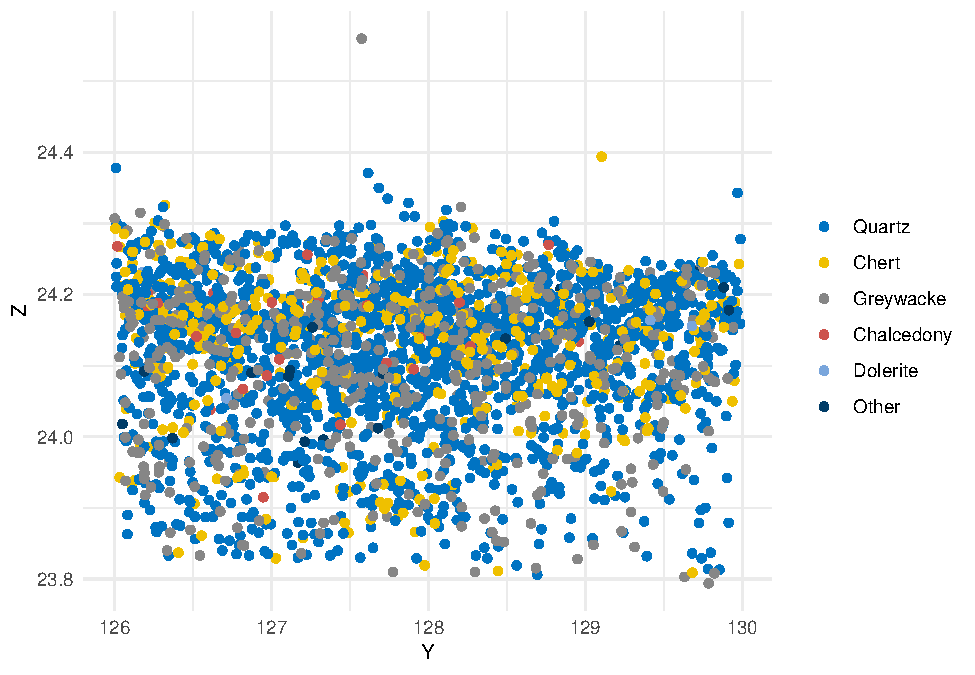
\includegraphics{thesis_files/figure-latex/spatialdistributionVB-1.pdf}
\caption{\label{fig:spatialdistributionVB}Spatial distribution of lithic artefacts (without chips) by raw material, on unit H.}
\end{figure}
However, when calculating the percentages of greywacke, chert and quartz and their relative frequencies by cubic meter of sediment (fig X) and plotting them by depth, there are significant differences in raw material distribution across time. From around 24.1 m upwards, there is a shift in quartz and chert frequencies, the latter increasing more than 10\% and quartz dropping from c.~50\% to nearly 30\%. Greywacke frequencies follow closely those of quartz.

This shift seems to be associated with other significant changes in the archaeological record, such as the abovementioned increase in the amount of lithic materials in top Layer 5 and Layer 4e, but also the appearance of Vale Comprido technology (image X). Furthermore, these two moments are stratigraphically correlated with two different chronological horizons, the first dated to c.~26 kcal BP at c.~23.9 m depth and associated with higher frequencies of quartz use, and the second dated to c.~24.7 kcal BP at around 24.1 m depth, associated with higher frequencies of chert and decrease in quartz use.
\begin{figure}
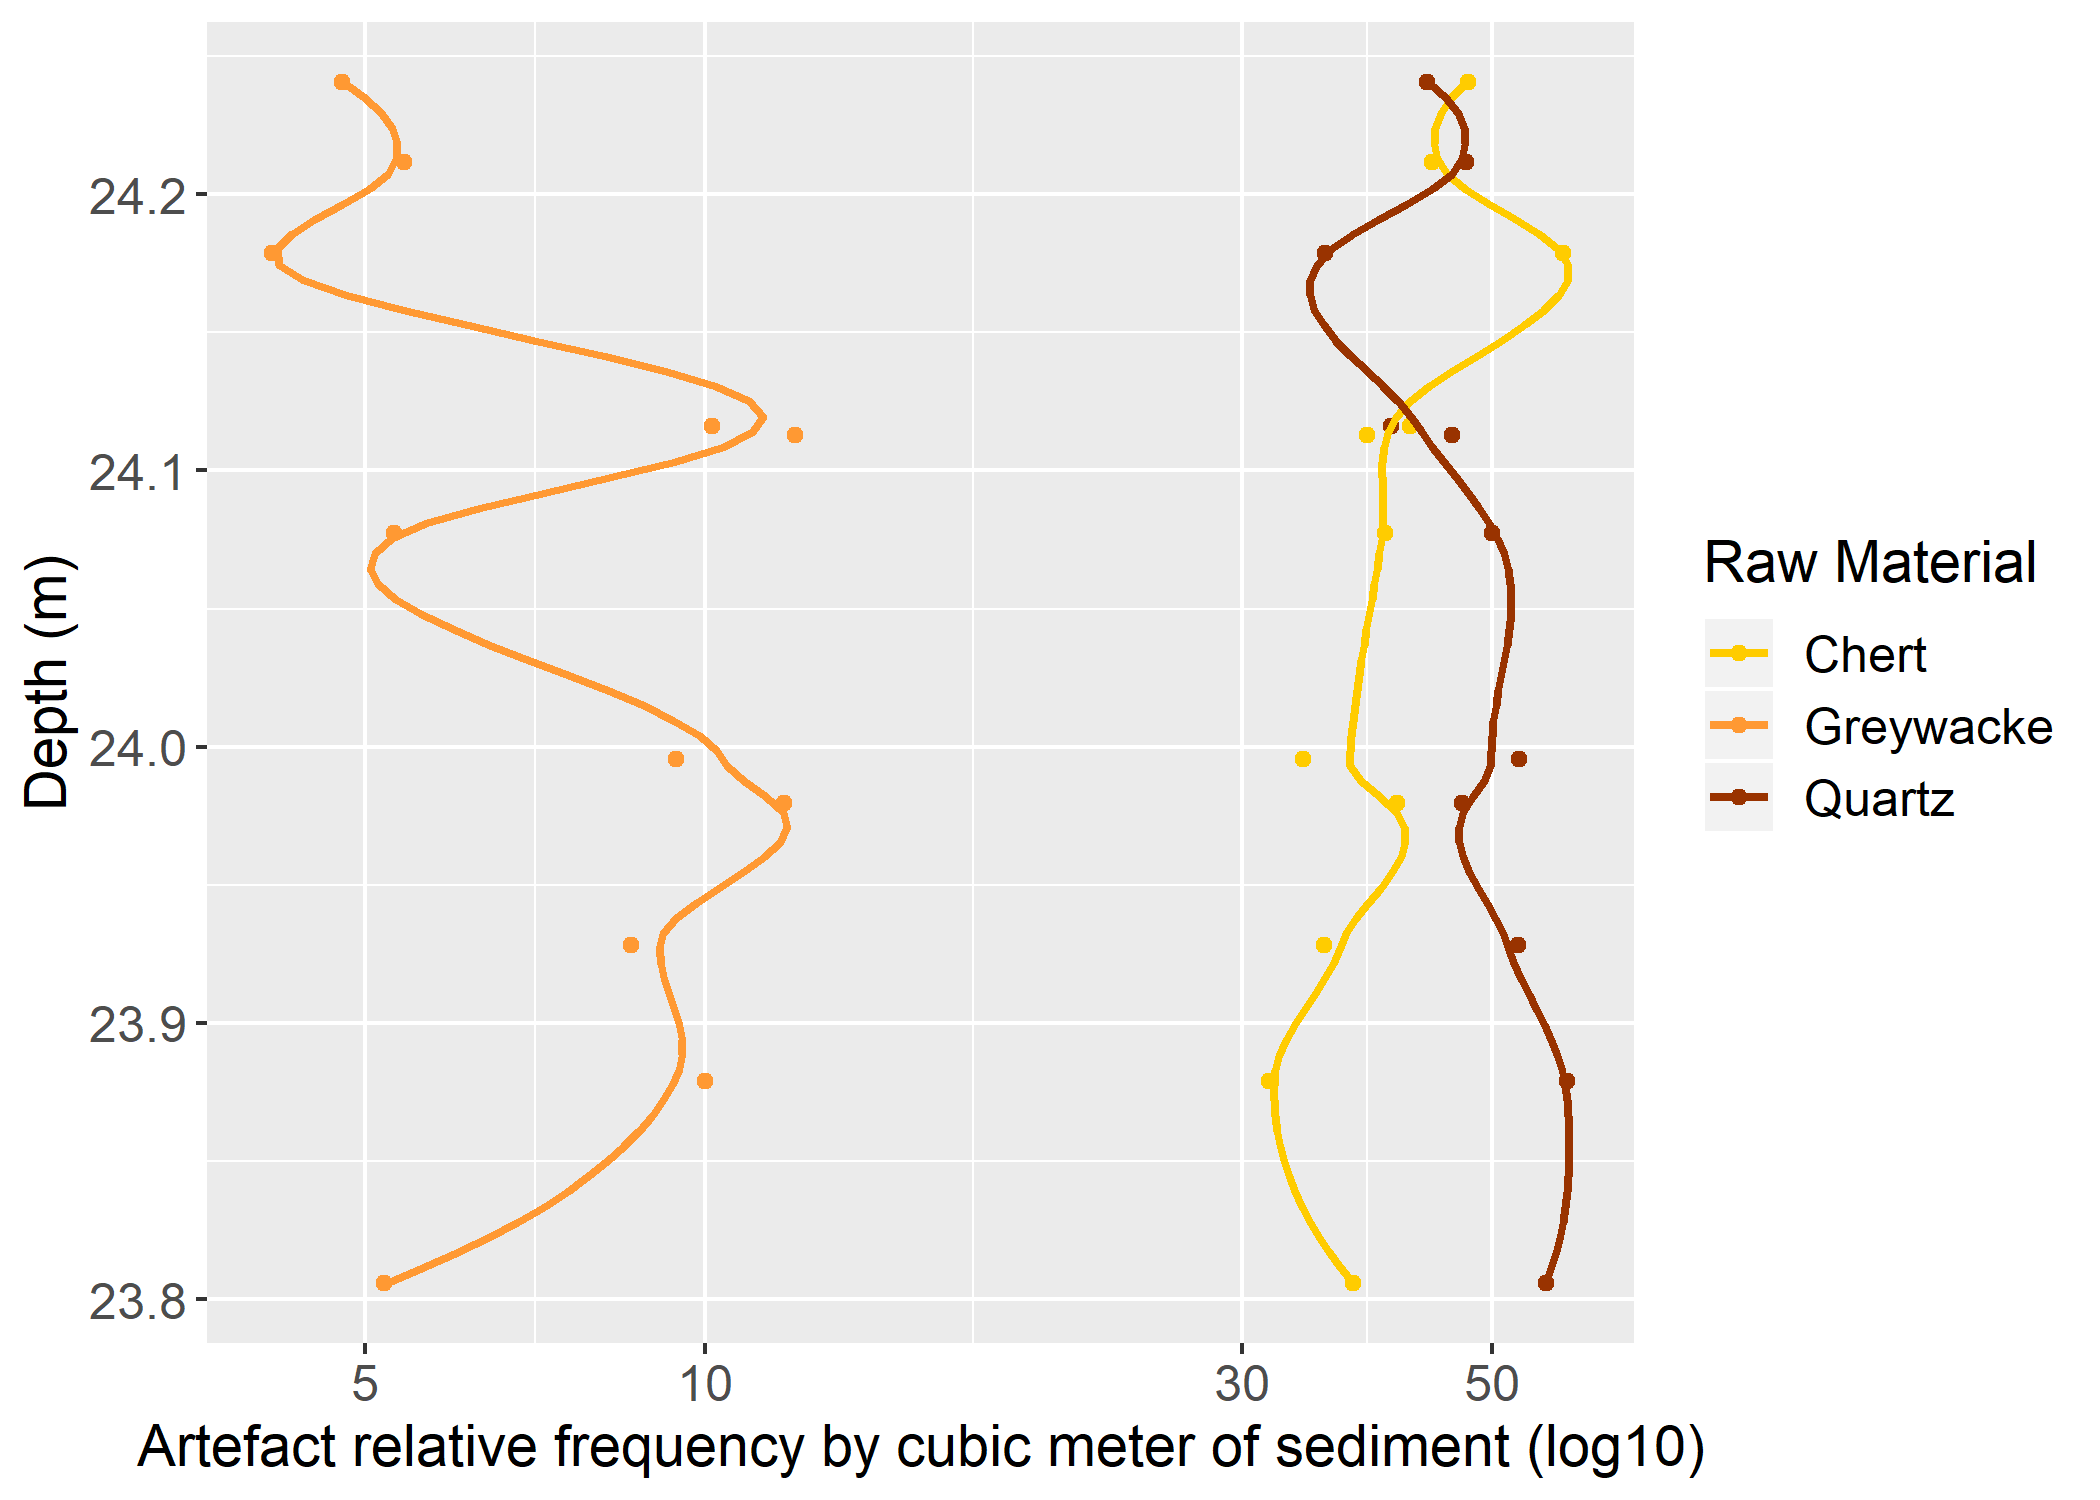
\includegraphics[width=1\linewidth]{figure/rm_cubic_meter} \caption{Complete debitage dispersion by depth}\label{fig:unnamed-chunk-11}
\end{figure}
As such, and given these chronological, density and raw material preference differences, it was decided that the assemblage would be analysed through its division in two analytical units, to better understand any possible technological differences: Lower 5, including all artefacts with Z values under 24.1; Upper 5/4E, including all artefacts with Z values of 24.1 and above. The value 24.1 was chosen for two reasons: 1) it is where the density of lithic materials seems to start; 2) its where the frequencies of quartz and chert start to shift beyond the already observed through the stratigraphic record of layers 5.

A total of 26711 pieces were analysed, 11094 from Lower 5 group and 15609 from Upper 5/4E, although most of these were chips (70.62\% from Lower 5 and 65.8\% from Upper 5/4E), followed by shatters, which make up c.~21.4\% and c.~24.5\% of the groups respectively.

For Lower 5, cores and debitage products represent a cumulative frequency of 7.95\%, whereas debitage debris represents 92\% of the total assemblage. For Upper 5/4E debitage products represent nearly 10\% of the group assemblage, while debris represent 90\%. These extremely high debris numbers can be mostly attributed to quartz, which may be explained not only by its knapping on the site, but also by its breakage patterns (especially when coarse), which might produce more waste than other raw materials.

Regarding debitage, blanks are the most represented class for both groups, with 1476 identified pieces, 4.5\% for Lower 5 and 6.18\% for Upper 5/4E, followed by blank fragments with an absolute count of 248 for Lower 5 and 336 for Upper 5/4E. Throughout the analysis, 167 retouched pieces were identified, 55 on Lower 5, representing 0.5\% of the group, and 112 on Upper 5/4E, with a frequency of 0.72\%, while retouched piece fragments composed a much smaller number (n = 7 for Lower 5 and n = 16 for Upper 5/4E).

Cores are also relatively frequent within the assemblage, with an absolute count of 123 cores, 46 for Lower 5 and 77 for Upper 5/4E, while core fragments are, alike the classes already referenced, in much smaller numbers (n = 11 and n = 16, respectively).
\begin{landscape}\begin{table}

\caption{\label{tab:general1}Technological class by raw material for Lower 5.}
\centering
\resizebox{\linewidth}{!}{
\begin{tabular}[t]{>{\bfseries}lrlrlrlrlrlrlrl}
\toprule
Class & Quartz (n) & Quartz (\%) & Chert (n) & Chert (\%) & Greywacke (n) & Greywacke (\%) & Dolerite (n) & Dolerite (\%) & Chalcedony (n) & Chalcedony (\%) & Other (n) & Other (\%) & Total & Total (\%)\\
\midrule
Anvil & 0 & 0\% & 0 & 0\% & 2 & 0.09\% & 0 & 0\% & 0 & 0\% & 0 & 0\% & 2 & 0.02\%\\
Blank & 281 & 3.58\% & 171 & 15.86\% & 44 & 2.08\% & 3 & 50\% & 6 & 37.5\% & 4 & 11.76\% & 509 & 4.59\%\\
BlankFrag & 132 & 1.68\% & 90 & 8.35\% & 23 & 1.09\% & 1 & 16.67\% & 1 & 6.25\% & 1 & 2.94\% & 248 & 2.24\%\\
Core & 18 & 0.23\% & 23 & 2.13\% & 3 & 0.14\% & 0 & 0\% & 1 & 6.25\% & 1 & 2.94\% & 46 & 0.41\%\\
CoreFrag & 2 & 0.03\% & 8 & 0.74\% & 0 & 0\% & 1 & 16.67\% & 0 & 0\% & 0 & 0\% & 11 & 0.1\%\\
\addlinespace
CorePreparProd & 1 & 0.01\% & 0 & 0\% & 0 & 0\% & 0 & 0\% & 0 & 0\% & 0 & 0\% & 1 & 0.01\%\\
Manuport & 0 & 0\% & 0 & 0\% & 2 & 0.09\% & 0 & 0\% & 0 & 0\% & 1 & 2.94\% & 3 & 0.03\%\\
RetouchedPiece & 15 & 0.19\% & 38 & 3.53\% & 1 & 0.05\% & 0 & 0\% & 1 & 6.25\% & 0 & 0\% & 55 & 0.5\%\\
RetouchedPieceFrag & 3 & 0.04\% & 4 & 0.37\% & 0 & 0\% & 0 & 0\% & 0 & 0\% & 0 & 0\% & 7 & 0.06\%\\
Shatter & 1754 & 22.36\% & 95 & 8.81\% & 507 & 23.96\% & 0 & 0\% & 5 & 31.25\% & 16 & 47.06\% & 2377 & 21.43\%\\
\addlinespace
Chip & 5638 & 71.88\% & 649 & 60.2\% & 1534 & 72.5\% & 1 & 16.67\% & 2 & 12.5\% & 11 & 32.35\% & 7835 & 70.62\%\\
Total & 7844 & - & 1078 & - & 2116 & - & 6 & - & 16 & - & 34 & - & 11094 & -\\
\bottomrule
\end{tabular}}
\end{table}
\end{landscape}
\begin{landscape}\begin{table}

\caption{\label{tab:general2}Technological class by raw material for Upper 5/4E.}
\centering
\resizebox{\linewidth}{!}{
\begin{tabular}[t]{>{\bfseries}lrlrlrlrlrlrlrl}
\toprule
Class & Quartz (n) & Quartz (\%) & Chert (n) & Chert (\%) & Greywacke (n) & Greywacke (\%) & Dolerite (n) & Dolerite (\%) & Chalcedony (n) & Chalcedony (\%) & Other (n) & Other (\%) & Total & Total (\%)\\
\midrule
Blank & 438 & 3.91\% & 407 & 19.53\% & 80 & 3.62\% & 14 & 60.87\% & 18 & 32.14\% & 8 & 34.78\% & 965 & 6.18\%\\
BlankFrag & 151 & 1.35\% & 155 & 7.44\% & 20 & 0.9\% & 3 & 13.04\% & 7 & 12.5\% & 0 & 0\% & 336 & 2.15\%\\
Burin spall & 0 & 0\% & 1 & 0.05\% & 0 & 0\% & 0 & 0\% & 0 & 0\% & 0 & 0\% & 1 & 0.01\%\\
Core & 32 & 0.29\% & 42 & 2.02\% & 1 & 0.05\% & 0 & 0\% & 0 & 0\% & 2 & 8.7\% & 77 & 0.49\%\\
CoreFrag & 4 & 0.04\% & 10 & 0.48\% & 0 & 0\% & 0 & 0\% & 0 & 0\% & 0 & 0\% & 14 & 0.09\%\\
\addlinespace
CorePreparProd & 1 & 0.01\% & 5 & 0.24\% & 0 & 0\% & 0 & 0\% & 0 & 0\% & 0 & 0\% & 6 & 0.04\%\\
Manuport & 0 & 0\% & 0 & 0\% & 5 & 0.23\% & 0 & 0\% & 0 & 0\% & 1 & 4.35\% & 6 & 0.04\%\\
RetouchedPiece & 34 & 0.3\% & 70 & 3.36\% & 2 & 0.09\% & 5 & 21.74\% & 1 & 1.79\% & 0 & 0\% & 112 & 0.72\%\\
RetouchedPieceFrag & 6 & 0.05\% & 9 & 0.43\% & 1 & 0.05\% & 0 & 0\% & 0 & 0\% & 0 & 0\% & 16 & 0.1\%\\
Shatter & 3006 & 26.81\% & 227 & 10.89\% & 563 & 25.46\% & 1 & 4.35\% & 15 & 26.79\% & 12 & 52.17\% & 3824 & 24.5\%\\
\addlinespace
Chip & 7540 & 67.25\% & 1158 & 55.57\% & 1539 & 69.61\% & 0 & 0\% & 15 & 26.79\% & 0 & 0\% & 10252 & 65.68\%\\
Total & 11212 & - & 2084 & - & 2211 & - & 23 & - & 56 & - & 23 & - & 15609 & -\\
\bottomrule
\end{tabular}}
\end{table}
\end{landscape}
\hypertarget{lapa-do-picareiro-2}{%
\subsection{Lapa do Picareiro}\label{lapa-do-picareiro-2}}

As previously discussed, the present assemblage, corresponding to layers U and T, seems to originate from two different moments of occupation of the cave, which were identified based on spatial distribution and raw material patterns, also having different dates for each of the moments. These patterns have been identified as Terminal Gravettian and Proto-Solutrean phases within the Proto-Solutrean transition model.

As such, and given the patterns, although the assemblage was analysed as a whole, for the statistic descriptive and multivariate analysis, the assemblage was separated into two groups: U/Lower T, which included all artefacts with depths inferior to 566.9 m or from levels U or T8 to T6 (Haws et al.~2019); Middle T, including all artefacts with depths equal or superior to 566.9 m of depth, or from the top 5 spits of level T. Any other artefact in the assemblage, which did not have a depth value or level was not considered in these results, since it lacked the needed information to contextualize its technological attributes.

The assemblage is composed of 376 pieces (with identifiable provenance), 196 from the U/Lower T phase and 180 from the Middle T group. In both phases, debitage waste is mostly composed of chips, which represent 49.4\% of the U/Lower T group and 37.2\% of the Middle T group. Alike Vale Boi, these values for debitage waste can be mostly explained by quartz, possibly related to the breakage patterns of this raw material.

The second most present class for both groups are blanks, which represent 14.2\% of the U/Lower T group and 37.2\% of the Middle T group, followed by blank fragments (13.7\% and 15.5\% respectively).Retouched pieces have relatively small frequencies, representing 3\% in U/Lower T and 2.7\% in Middle T. Cores have a frequency of 1\% in the U/Lower T group (n=2) and 2.7\% in the Middle T (n=5) and there is the presence of 1 core preparation product in the U/Lower T group.
\begin{table}

\caption{\label{tab:generalTG}Technological class by raw material (U/Lower T phase).}
\centering
\resizebox{\linewidth}{!}{
\begin{tabular}[t]{>{\bfseries}lrlrlrlrl}
\toprule
Class & Quartz (n) & Quartz (\%) & Chert (n) & Chert (\%) & Other (n) & Other (\%) & Total & Total (\%)\\
\midrule
Blank & 30 & 20.83\% & 24 & 53.33\% & 1 & 14.29\% & 55 & 28.06\%\\
BlankFrag & 22 & 15.28\% & 4 & 8.89\% & 1 & 14.29\% & 27 & 13.78\%\\
Core & 2 & 1.39\% & 0 & 0\% & 0 & 0\% & 2 & 1.02\%\\
CorePreparProd & 0 & 0\% & 1 & 2.22\% & 0 & 0\% & 1 & 0.51\%\\
Manuport & 0 & 0\% & 0 & 0\% & 1 & 14.29\% & 1 & 0.51\%\\
\addlinespace
RetouchedPiece & 1 & 0.69\% & 5 & 11.11\% & 0 & 0\% & 6 & 3.06\%\\
Shatter & 4 & 2.78\% & 1 & 2.22\% & 2 & 28.57\% & 7 & 3.57\%\\
Chip & 85 & 59.03\% & 10 & 22.22\% & 2 & 28.57\% & 97 & 49.49\%\\
Total (RM) & 144 & - & 45 & - & 7 & - & 196 & -\\
\bottomrule
\end{tabular}}
\end{table}
\begin{table}

\caption{\label{tab:generalPR}Technological class by raw material (Middle T phase).}
\centering
\resizebox{\linewidth}{!}{
\begin{tabular}[t]{>{\bfseries}lrlrlrlrl}
\toprule
Class & Quartz (n) & Quartz (\%) & Chert (n) & Chert (\%) & Other (n) & Other (\%) & Total & Total (\%)\\
\midrule
Blank & 19 & 19\% & 46 & 63.01\% & 2 & 28.57\% & 67 & 37.22\%\\
BlankFrag & 19 & 19\% & 9 & 12.33\% & 0 & 0\% & 28 & 15.56\%\\
Core & 2 & 2\% & 2 & 2.74\% & 1 & 14.29\% & 5 & 2.78\%\\
RetouchedPiece & 0 & 0\% & 5 & 6.85\% & 0 & 0\% & 5 & 2.78\%\\
Shatter & 3 & 3\% & 2 & 2.74\% & 3 & 42.86\% & 8 & 4.44\%\\
\addlinespace
Chip & 57 & 57\% & 9 & 12.33\% & 1 & 14.29\% & 67 & 37.22\%\\
Total (RM) & 100 & - & 73 & - & 7 & - & 180 & -\\
\bottomrule
\end{tabular}}
\end{table}
\hypertarget{raw-materials}{%
\section{Raw materials}\label{raw-materials}}

Raw material use and availability, specifically abundance and quality, stand as important factors for understanding the organization of technology, as it may affect decisions regarding tool design and conservation of such tools (Andrefsky, 1994), as well as mobility and niche expansion (Cascalheira, 2013). This quality is connected to both the raw material's fracture mechanics and their intrinsic mineral characteristics, such as the size of their grain, homogeneity (Andrefsky, 1994) or even hardness (Kempson \& Wadley, 2011), which allow the knapper predictability over the outcome (Andresfsky 2005).

As such, there are a number of stones which are constant throughout the archaeological record for having the necessary properties described above. Stones or minerals characterized by high frequencies of silica, such as chert or quartz, allow for good fracture predictability, while other materials with less homogeneity may progressively result in less predictable characteristics (Andresfsky 2005). Thus, despite the raw material variability within the pre-historical archaeological record, linked to its availability and geomorphological contexts of the sites, the selection is often coherent regarding fracture mechanics, where predictable conchoidal fractures are preferred (Inizan et al., 1999; Tixier \& Inizian, 1980) (Andrefsky 2005).

This pattern is also observable in Vale Boi. Previous studies have shown that, throughout most levels of human occupation in Vale Boi, chert, quartz and greywacke (all three characterized by a conchoidal fracture, although greywacke is often coarse and more unpredictable) were the most frequently used (Bicho, Cascalheira, \& Marreiros, 2012; Cascalheira, 2010; Marreiros, 2009) (Pereira et al 2016), these being available at a regional and local scale . Although their presence is documented throughout the archaeological levels, each occupation might differ in the frequency of their use, but following a pattern where chert is the primary raw material used for knapping (Cascalheira, 2010). The preferential use of these raw materials is also reported for other sites in Portugal from the Upper and Middle Paleolithic (Almeida, 2000; Pereira \& Benedetti, 2013; Zilhão, 1997).
The same patterns seem to generally apply to the present assemblages, both Vale Boi level 4E and 5, and Lapa do Picareiro for levels U and T, where quartz and chert are still the predominant raw materials (Vale Boi also showing high frequencies of greywacke and higher raw material variability), although in different frequencies from other layers.
Criteria used for raw material analysis focused on the identification of broader groups of stones and minerals (e.g.~chert or quartz), based on their general observable characteristics, without focusing on the particular features within each raw material. As such, aside from quartz, no other raw material was subdivided by grain or colouration differences.

\hypertarget{vale-boi-3}{%
\subsection{Vale Boi}\label{vale-boi-3}}

The raw materials identified in layers 4E and 5 in the present study were quartz (subdivided in rock crystal, fine, medium and coarse quality), chert, greywacke, dolerite, chalcedony, all other less represented raw materials having been collapsed in a variable named ``Other''.

\hypertarget{quartz}{%
\subsubsection{Quartz}\label{quartz}}

Quartz is, unlike other raw materials in this study, a mineral (Inizan et al.~1999), characterized by either a smoky grey colouration or lack of colour, glassiness, hardness and conchoidal fracture (Haldar and Tisljar 2014).

The number of chips and shatter in quartz in the total assemblage are, as seen in table X, extremely high, both in its representativity within the raw material, where it represents nearly 94.2\% for Lower 5 and 94\% for Upper 5/4E of all quartz, and through the comparison of its absolute numbers with other raw materials.

Despite the low frequencies represented on the table, there is a large number of blanks made in quartz (n=281 for Lower 5 and 438 for Upper 5/4E) compared to the rest of classes, as well as cores (n=18 for Lower 5 and n=32 for Upper 5/4E) and retouched pieces (n=15 for Lower 5 and n=34 for Upper 5/4E). These patterns are well represented in figure X, where the percentages of quartz (excluding shatter and chips), represent a great fraction of the total assemblage: more than 50\% in the Lower 5 phase and around 45\% in Upper 5/4E.

Alike other raw materials, most quartz does not show the presence of cortex, with nearly 95\% of all materials having 0\% cortex. When it is present, around 72\% seems to come from cobbles or pebbles. These patterns are similar for both Lower 5 and Upper 5/4E.

As mentioned before, quartz was divided into groups regarding size of grain or, in case of rock crystal, regarding colouration as well. Analysing the artefact class frequency through the different identified types of quartz quality confirmed a pattern which was already expected: use of fine and medium quality quartz was mainly dedicated for the production of blanks (52.7\% and 32.4\% for Lower 5, and 50.9\% and 29.7\% for Upper 5/4E, respectively) and retouched products (66.7\% and 26.7\% for Lower 5, and 55.9\% and 44.1\% for Upper 5/4E). Alike coarse quality quartz, no retouched pieces were identified in rock crystal, this type of quartz having a small presence in the total assemblage.
\begin{table}[!h]

\caption{\label{tab:quartzquality1}Quartz quality by class (Lower 5).}
\centering
\resizebox{\linewidth}{!}{
\begin{tabular}[t]{>{\bfseries}llllll}
\toprule
Quartz quality & Blank & Core & CorePreparProd & RetouchedPiece & Total\\
\midrule
QuartzQuality, n (\%) &  &  &  &  & \\
Coarse & 40 (14.2) & 5 (27.8) & 0 (0.0) & 1 (6.7) & 46 (14.6)\\
Fine & 148 (52.7) & 6 (33.3) & 0 (0.0) & 10 (66.7) & 164 (52.1)\\
Medium & 91 (32.4) & 7 (38.9) & 1 (100.0) & 4 (26.7) & 103 (32.7)\\
RockCrystal & 2 (0.7) & 0 (0.0) & 0 (0.0) & 0 (0.0) & 2 (0.6)\\
\bottomrule
\end{tabular}}
\end{table}
\begin{table}[!h]

\caption{\label{tab:quartzquality2}Quartz quality by class (Upper 5/4E).}
\centering
\resizebox{\linewidth}{!}{
\begin{tabular}[t]{>{\bfseries}llllll}
\toprule
Quartz quality & Blank & Core & CorePreparProd & RetouchedPiece & Total\\
\midrule
QuartzQuality, n (\%) &  &  &  &  & \\
Coarse & 82 (18.7) & 9 (28.1) & 0 (0.0) & 0 (0.0) & 91 (18.0)\\
Fine & 223 (50.9) & 7 (21.9) & 0 (0.0) & 19 (55.9) & 249 (49.3)\\
Medium & 130 (29.7) & 16 (50.0) & 1 (100.0) & 15 (44.1) & 162 (32.1)\\
RockCrystal & 3 (0.7) & 0 (0.0) & 0 (0.0) & 0 (0.0) & 3 (0.6)\\
\bottomrule
\end{tabular}}
\end{table}
\hypertarget{chert}{%
\subsubsection{Chert}\label{chert}}

Chert, as defined by Haldar and Tisljar (2014), is a cryptocrystalline solid-silicon rock, characterized by sharp fractures, referred to as flint whenever it is ``(\ldots) used as artifacts, weapons and tools of prehistoric man.''

This raw material shows high frequencies of blanks (15.8\% for Lower 5 and 19.5\% for Upper 5/4E) when compared to every other class, excluding chips. These latter represent more than 50\% of the chert, although at much smaller quantities than in quartz, with an absolute number of 649 chips for Lower 5 and 1158 for Upper 5/4E.

Although chert shows smaller numbers for blanks (n=171 for Lower 5 and n=407 for Upper 5/4E) and blank fragments (n=90 for Lower 5 and n=155 for Upper 5/4E) compared to quartz, there is a large quantity of cores which represent 2.1\% of total chert in Lower 5 and 2\% in Upper 5/4E, showing that both raw materials were expediently used in these layers. However, table X shows an obvious difference in ratio between chert blanks and quartz blanks between Lower 5 and Upper 5/4E, with the latter showing a higher ratio of chert blanks comparatively to Upper 5/4E. This can also be seen in figure X, where chert on Upper 5/4E shows a frequency of around 30\% (excluding chips and shatter), thus being the second most used raw material, while on Upper 5/4E it represents almost 50\%, a higher frequency than quartz, and thus becoming the first most used raw material in the group.

Regarding retouched pieces, these represent more than 3\% of chert for both phases, a number far higher than those in other raw materials, thus showing chert, although less present than quartz in blanks (although barely in Upper 5/4E), might have been preferentially used for tools.

Regarding cortex, chert shows the biggest variability of cortex presence percentages in both phases, although there continues to be a clear dominance of debitage with 0\% cortex, which was already expected, following the process of the knapping sequence, where only the first blanks removed from an unmodified block will be entirely cortical, showing increasingly less cortex for posterior removals (Andrefsky 2005). This variability in cortex presence is accompanied in variability of cortex types, with the presence of both cobble and outcrop sources, although almost 85\% of cortex didn't show enough characteristics to be identified with certainty.

\hypertarget{greywacke}{%
\subsubsection{Greywacke}\label{greywacke}}

Greywacke is a variety of sandstone, often characterized by its hardness, dark colour and poorly sorted grains of quartz and feldspar (Haldar and Tisljar 2014). At Vale Boi, this raw material is highly heterogenous, with a wide variety of grain sizes and colourations.

It is best represented by debitage waste, with nearly 25\% of shatter and around 70\% of chips, for both Lower 5 and 2, with relatively low numbers for blanks (n=44 for Lower 5 and n=80 for Upper 5/4E) and cores (n=3 for Lower 5 and 1 for Upper 5/4E). The same applies for the retouched pieces, with an absolute number of 3 in the total assemblage, one of which is a Vale Comprido point in Upper 5/4E.

When the chips and shatter are removed, greywacke has a representation of less than 12\% in the total assemblage (with a smaller frequency in Upper 5/4E), making it the third most used raw material in the assemblage, although with a wide difference in frequency when compared to chert and quartz.

Similarly to the other raw materials, there is, for both phases, the predominance of debitage without cortex, although there is a certain variability in cortex presence, even if in smaller frequencies than the observed in chert. Alike quartz, most cortex was identified as cobble.

\hypertarget{dolerite}{%
\subsubsection{Dolerite}\label{dolerite}}

Dolerite is a volcanic igneous rock, occurring mostly in dykes, varying between coarse and fine textures, and often having a dark, grey or greyish-green colouration (Haldar and Tisljar 2014; Wadley and Kempson 2011; Belmiro 2018). In the Algarve, its presence is registered in two main areas : , and near Sagres, southwest of the Algarve, as outcrops within the Messejana fault (Belmiro 2018).

This raw material was first identified as jasper when excavating the levels referring to the Proto-Solutrean occupation of Vale Boi, in the terrace area (units J-L), prior to 2012 (Marreiros 2009), being characterized by a reddish-brown coloration and fine texture, with a conchoidal fracture. Despite this coloration, which is also present in jasper, a red coloured variety of chalcedony, the raw material was later identified as dolerite, and its colouration explained by the presence of a reddish patina which would have altered the original rock, by processes of iron mineral oxidation through contact with terra rossa (Belmiro 2018).

The analysis of a thin section obtained from a dolerite fragment from the present assemblage allowed the characterization of this raw material, through its visible features and petrography.

The reddish coloration was confirmed to be an exterior patina, no more than 1 mm thick, through the whole extension of the piece. The actual rock still displays a fine texture but with an opaque black coloration.

Results from the petrographic analysis done through the observation of the thin section using a polarizing microscope revealed the presence of several minerals, such as feldspar, plagioclase, quartz, small quantities of silica, little presence of mica and iron oxide, which are in concordance with the mineral composition of dolerite or possibly hornfels (Wadley and Kempson 2011). Furthermore, the feldspar minerals showed the presence of ondulatory extinction, a deformation that takes place whenever certain minerals are exposed to high temperatures (Frost and Frost 2014), thus indicating that the raw material is highly metamorphized.

Regarding the differentiation between dolerite and hornfels, although these two rocks have different origins, the latter being of volcanic igneous origin, considered a contact metamorphic rock (Haldar and Tisljar 2014), they share enough physical and mineral characteristics (whenever the dolerite has a fine texture) to hinder their precise identification. Literature most often uses other methods to differentiate them, such as FTIR, XRF, by understanding not the mineral composition (which is essentially the same) but the ratio of components presence. This matter is further complexified by understanding that hornfels might originate from metamorphized igneous rocks, several sources of hornfels attributed to dolerite dikes (Wadley and Kempson 2011; Hallinan and Shaw 2017).

Given this difficulty, although the present analysis will use the term dolerite, for their reported similarities in terms of texture, grain size and fracture, further chemical studies need to be done in order to confirm whether the raw material is dolerite or possibly hornfels. Regarding the latter, there is also the presence of hornfels outcrops and rounded pebbles in the Algarve, near the southwestern coast , thus strengthening the hypothesis that this raw material, whether dolerite or hornfels, is local.

Understanding the interior look of dolerite allowed, during the second moment of analysis, to identify other products in the same raw material, which hadn't previously been identified for the lack of the same reddish patina. This patina also appears throughout the assemblage, mostly on greywacke, although without forming the same thick layer visible on some dolerite pieces. This may be explained by the inherent mineral characteristics of this type of raw material.

The presence of this patina in several degrees of intensity, preferentially in dolerite (as a thick patinated layer) and greywacke, its presence in not only finished complete artefacts, but also flake fragments or shatter, and its occurrence also reported in the literature as a process frequently affecting raw materials like hornfels (e.g.~Hallinan and Shaw 2017), suggests that it is, in fact, the result of geological and chemical processes affecting these raw materials. Its absence from other raw materials, like chert or quartz, may simply reflect the inherent mineral properties of these materials.

Dolerite is an unprecedented raw material in the site of Vale Boi, appearing only in layers 4E and 5 of the Terrace and Proto-Solutrean levels of the Slope area. The most striking characteristic of this raw material in Vale Boi is the low presence of chips or shatter (n=1 each), but instead high frequencies of blanks (50\% in Lower 5 and 60.8\% in Upper 5/4E) and blank fragments (16.6\% in Lower 5 and 13\% in Upper 5/4E). Upper 5/4E, unlike Lower 5 in which no dolerite retouched piece was identified, shows the presence of 5 retouched pieces, some of which are Vale Comprido points. In fact, this raw material seems to have been used preferentially at Vale Boi for the production of these types of points, a pattern already observed in previous works (Marreiros 2009), where three of five Vale Comprido points were identified as dolerite (or jasper originally).

The absence of cores, with only 1 core fragment identified in the Lower 5 group, and low quantity of debitage waste may be explained by the transportation of finished pieces or blanks, without carrying out knapping activities with this raw material at the site. This interpretation is, however, truncated by this study's phase analysis. As the identification of the inner aspect of dolerite was only achieved at the start of the second phase, which as referred before, consisted of the analysis of all cores and debitage products with a wider database, shatter and chips were not revisited, thus not allowing for the possible identification of possible unpatinated dolerite within those classes, which might have been mistaken for fine grained greywacke. This caveat does not, however, seem to influence the patterns regarding blank and retouched piece frequency.

\hypertarget{chalcedony}{%
\subsubsection{Chalcedony}\label{chalcedony}}

Chalcedony is a type of cryptocrystalline quartz, characterized by a waxy and glossy appearance, ranging from a variety of possible colourations (Haldar and Tisljar 2014), although white is the only present variety in the assemblage. The chalcedony in levels 4E and 5 can also be characterized by the presence of inclusions, making this raw material poorly homogeneous.

Results indicate it may have been mainly used for the production of blanks, which represent 37.5\% of chalcedony in Lower 5 and 32.1\% in Upper 5/4E, with a rather small representation of retouched pieces (n=2), which include a Vale Comprido point in the Upper 5/4E group. The presence of a core in Lower 5 may indicate the knapping of this raw material at the site, as well as the presence of shatter and chips, although in small numbers (less than 5 each for Lower 5 and n=15 each for Upper 5/4E).

Compared to other raw materials, chalcedony has the lowest frequencies of cortex, in both phases, with almost 100\% of all artefacts (except shatter and chips) having 0\% cortex, which, connected to its low representativity in the assemblage (figure X) might suggest the raw material was not frequently brought to the site and knapped for obtaining blanks and tools, possibly due to its poor quality and abundance of inclusions and flaws.
\begin{figure}
\centering
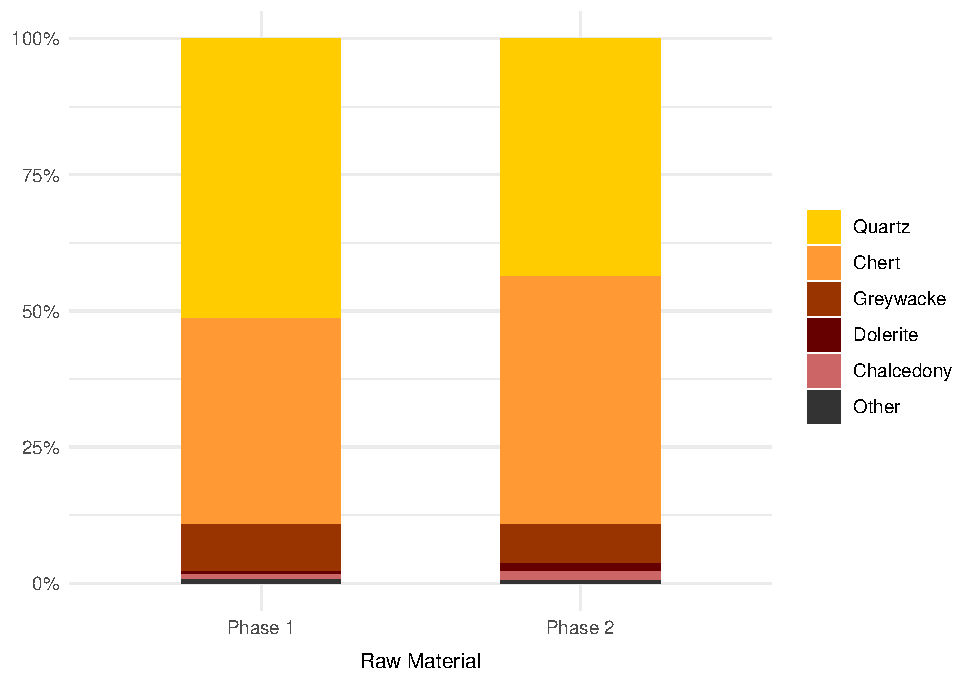
\includegraphics{thesis_files/figure-latex/rmvb-1.pdf}
\caption{\label{fig:rmvb}Raw material \% per phase without chips or shatter.}
\end{figure}
\begin{figure}
\centering
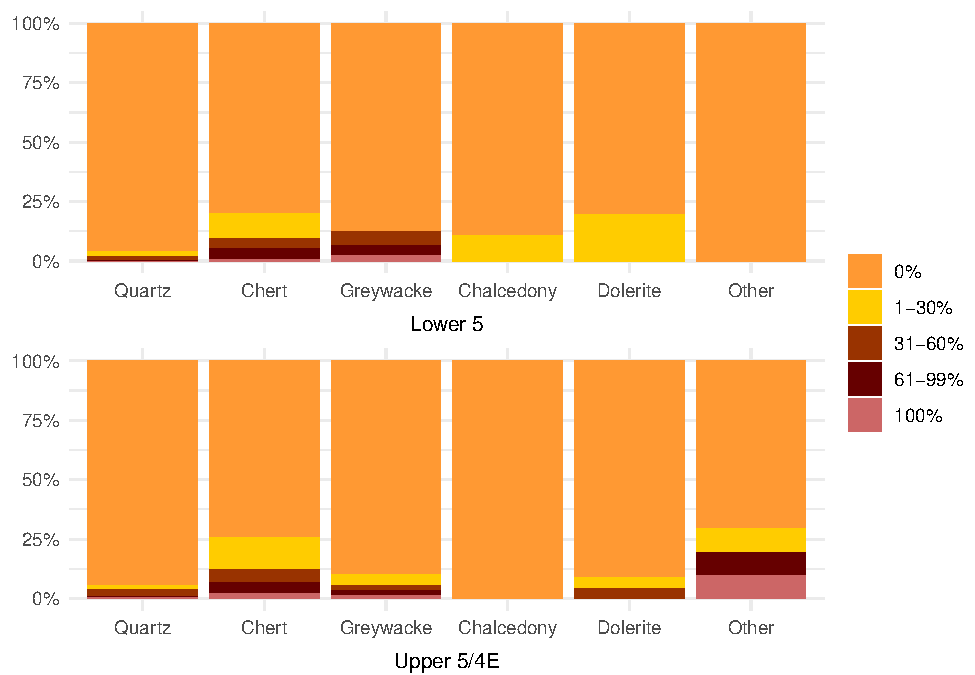
\includegraphics{thesis_files/figure-latex/rmcortex-1.pdf}
\caption{\label{fig:rmcortex}Cortex \% by raw material, without chips and shatterfor Lower 5 and 2.}
\end{figure}
\begin{table}

\caption{\label{tab:cortextab1}Cortex type and localization by raw material (Lower 5).}
\centering
\resizebox{\linewidth}{!}{
\begin{tabular}[t]{>{\bfseries}lllll}
\toprule
Cortex attributes & Quartz & Chert & Greywacke & Total\\
\midrule
CortexType, n (\%) &  &  &  & \\
Cobble & 15 (83.3) & 5 (8.5) & 7 (77.8) & 27 (31.0)\\
Indeterminate & 2 (11.1) & 50 (84.7) & 0 (0.0) & 53 (60.9)\\
Outcrop & 1 (5.6) & 4 (6.8) & 2 (22.2) & 7 (8.0)\\
\bottomrule
\end{tabular}}
\end{table}
\begin{table}

\caption{\label{tab:cortextab2}Cortex type and localization by raw material (Upper 5/4E).}
\centering
\resizebox{\linewidth}{!}{
\begin{tabular}[t]{>{\bfseries}lllllll}
\toprule
Cortex attributes & Quartz & Chert & Greywacke & Dolerite & Other & Total\\
\midrule
CortexType, n (\%) &  &  &  &  &  & \\
Cobble & 30 (81.1) & 11 (6.7) & 9 (81.8) & 2 (100.0) & 3 (100.0) & 55 (25.3)\\
Indeterminate & 4 (10.8) & 123 (75.0) & 2 (18.2) & 0 (0.0) & 0 (0.0) & 129 (59.4)\\
Outcrop & 3 (8.1) & 30 (18.3) & 0 (0.0) & 0 (0.0) & 0 (0.0) & 33 (15.2)\\
\bottomrule
\end{tabular}}
\end{table}
\hypertarget{lapa-do-picareiro-3}{%
\subsection{Lapa do Picareiro}\label{lapa-do-picareiro-3}}

Comparatively to Vale Boi, Lapa do Picareiro shows less raw material variability, which might be explained by the lithology of the area, already explored in other works, showing similar raw material presence patterns (Almeida, 2000; Zilhão, 1997). As such, during the analysis, the main raw materials identified were quartz and chert, with the sporadic occurrence of other raw materials, mainly comprised of quartzite.

\hypertarget{quartz-1}{%
\subsubsection{Quartz}\label{quartz-1}}

The number of chips in quartz, as seen on table X, is extremely high, representing nearly 60\% of this raw material in both groups, although the other debitage waste class shows much smaller numbers (n=4 for U/Lower T and n=3 for Middle T). Comparatively, blanks are the second most present class in quartz, with a frequency of 20\% (n=30) for the U/Lower T group, closely followed by blank fragments, which represent 15.2\%, a relatively high fragmentation percentage compared to the total number of complete pieces. For the Middle T group, blanks and blank fragments show exactly the same frequencies, represing within quartz pieces 19\%. Although in small numbers, quartz shows the highest number of cores (n=4, 2 in each group) from all raw materials, but a number of retouched pieces much smaller than the one in chert (n=1).

Despite the large quantity of chips, quartz is still well represented in its other classes, as seen in figure X, although in variable degrees, depending on the stage. While during the U/Lower T stage quartz (without chips) has a representativity of nearly 60\% of the total assemblage, during the Middle T occupation this frequency drops to around 37\%.

Regarding cortex, quartz shows frequencies as low as 6\% for cortex presence on the U/Lower T group, 12.5\% on the Proto-Solutrenan, being mostly composed of pieces without the presence of cortex. Whenever present, however, cortex reveals a cobble source for this raw material.

As mentioned before, quartz was also categorized regarding grain quality and colouration. For both the U/Lower T group and Middle T, it is possible to observe a majority of fine quality quartz and rock crystal for both cores and blanks, with barely any presence of medium and coarse quality quartz, the latter inexistent on the Middle T group. One observable difference between the two groups is in the percentages of rock crystal and fine quality: on the U/Lower T, fine quality quartz represents 56\% of quartz, while rock crystal has a frequency of nearly 41\%; for Middle T, these percentages change, as fine quality quartz represents 37\%, against 54\% of rock crystal. Finally, the identified retouched piece was made in fine quality quartz.
\begin{table}

\caption{\label{tab:quartzqualityTG}Quartz quality by class (Terminal Gravettian).}
\centering
\resizebox{\linewidth}{!}{
\begin{tabular}[t]{>{\bfseries}llllll}
\toprule
Quartz quality & Blank & Core & RetouchedPiece & Shatter & Total\\
\midrule
QuartzQuality, n (\%) &  &  &  &  & \\
Coarse & 0 (0.0) & 0 (0.0) & 0 (0.0) & 1 (25.0) & 1 (1.7)\\
Fine & 16 (53.3) & 1 (50.0) & 1 (100.0) & 3 (75.0) & 33 (55.9)\\
Medium & 1 (3.3) & 0 (0.0) & 0 (0.0) & 0 (0.0) & 1 (1.7)\\
RockCrystal & 13 (43.3) & 1 (50.0) & 0 (0.0) & 0 (0.0) & 24 (40.7)\\
\bottomrule
\end{tabular}}
\end{table}
\begin{table}

\caption{\label{tab:quartzqualityPR}Quartz quality by class (Middle T).}
\centering
\resizebox{\linewidth}{!}{
\begin{tabular}[t]{>{\bfseries}lllll}
\toprule
Quartz quality & Blank & Core & Shatter & Total\\
\midrule
QuartzQuality, n (\%) &  &  &  & \\
Fine & 7 (36.8) & 1 (50.0) & 1 (33.3) & 9 (37.5)\\
Medium & 1 (5.3) & 0 (0.0) & 1 (33.3) & 2 (8.3)\\
RockCrystal & 11 (57.9) & 1 (50.0) & 1 (33.3) & 13 (54.2)\\
\bottomrule
\end{tabular}}
\end{table}
\hypertarget{chert-1}{%
\subsubsection{Chert}\label{chert-1}}

This raw material is characterized by a high frequency of blanks (53.3\% for U/Lower T and 63\% for Middle T), with only a cumulative percentage of 24.4\% and 15\% for debitage waste, the U/Lower T and Middle T groups respectively, which might be related to chert's breakage patterns, producing less waste than quartz. Likewise, blank fragments are also poorly represented comparatively to quartz, with an absolute count of 4 for U/Lower T and 9 for the Middle T phase, representing only 8.8\% and 12.3\% of the chert. Although there are few cores in chert (n=2), retouched pieces have a relatively high frequency within the raw material (11.1 on U/Lower T and 6.85\% on Middle T), and as seen above, most of the retouched piece total, thus hinting this raw material might have been used preferentially for the manufacture of formal tools.

Regarding cortex, chert shows mostly products without cortex, a pattern further present in the Middle T group. Whenever cortex is present however, its source was indeterminate, although a few pieces allowed to track its source to outcrops.

Although chert was not firstly classified regarding its visible characteristics, throughout the analysis, it seemed apparent there were several groups with identical colours and grains, which might have belonged to the same nodule. As such, these groups were individualized posteriorly, adding a variable to the database called ``ChertType'' which included codes for each identified type of chert, which can be seen on table X.
\begin{table}

\caption{\label{tab:cherttable}Identified chert types. Description is mostly based on colours and colouration patterns, following the Munsel manual of color chart (Munsel Color (Firm) 2010).}
\centering
\begin{tabular}[t]{>{\bfseries}l>{\raggedright\arraybackslash}p{10cm}}
\toprule
Chert Type & Description\\
\midrule
RM1 & Fine grain, 2.5Y 7/6 and 6/6 (yellow and olive yellow) translucent color with opaque smoke-like patterns.\\
RM2 & Mostly 5YR 4/2 (dark reddish gray) and 4/3 (reddish brown) colouration, with 1mm 10YR 7/3 (very pale brown) dots and bigger 0.5 to 1 mm circular 10YR 7/2 (light gray) inclusions with coarser texture.\\
RM3 & Coarser texture, with veins and fog-like patterns with colour mix of 10YR 8/3, 7/3 (very pale brown), 7.5YR 7/3 (pink), 5YR 7/4 (pink) and 10YR 5/3 brown.\\
RM4 & Mostly 2.5Y 8/1 (white) with interior translucent areas.\\
RM5 & 2.5Y 6/2 (light brownish gray), closer to cortex 10YR 8/2 and 8/3 (very pale yellow) with circular 0.5 mm marks of 10YR 7/2 /(light gray) and 5Y 5/1 (gray) dots.\\
\addlinespace
RM6 & 10YR 8/3 (very pale brown) on borders, center fog-like pattern with mix of 10YR 4/2,3/3 (dark brown), 2.5Y 6/3 (light yellowish brown) and 5/1 (gray).\\
RM7 & Stripped-like ondulating pattern with several tonalities: 5YR 7/3, 8/3 (pink), 6/6 (reddish yellow), 7/1 (light gray), with certain areas with 7.5YR 7/8 (reddish yellow).\\
\bottomrule
\end{tabular}
\end{table}
After its identification, it was attempted to refit the pieces in each group, but due to the high level of modification and edge damage of each piece, this was not possible. However, using the spatial data, each group was plotted in order to understand any spatial restriction or relationship that might help identify a specific knapping behaviour (fig X).

Although most groups seem to show no particular spatial restriction or pattern when plotted, RM6 seems to have a good concentration of materials, starting at depth 567 m, which corresponds to the second spit of what is considered the Middle T levels, matching also with the highest quantity of chert in the plot.
\begin{figure}
\centering
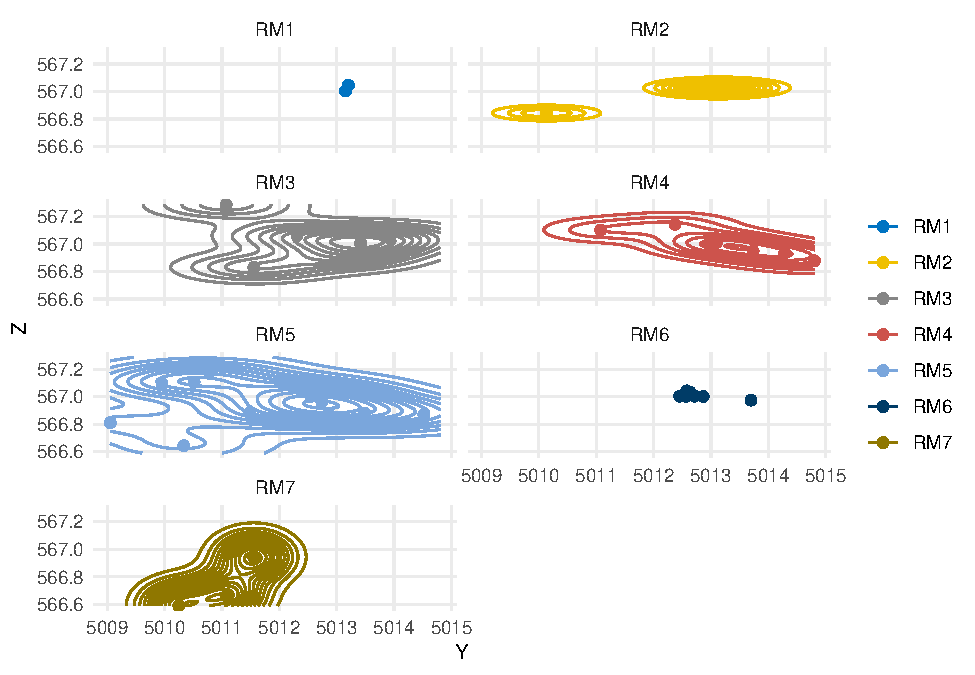
\includegraphics{thesis_files/figure-latex/chertspatial-1.pdf}
\caption{\label{fig:chertspatial}Types of chert spatial dispersion}
\end{figure}
\begin{figure}
\centering
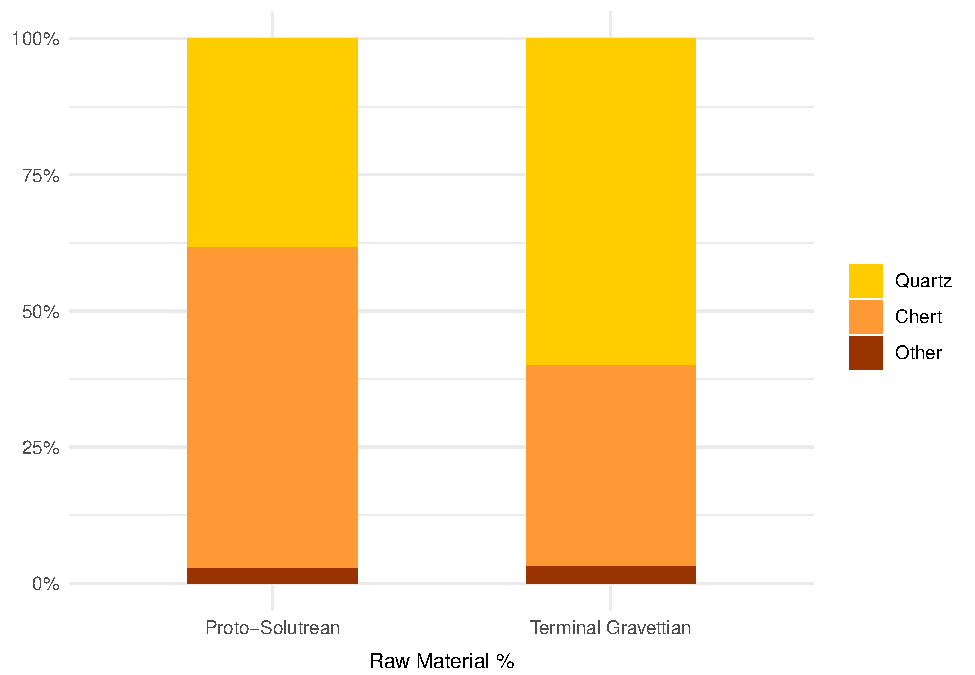
\includegraphics{thesis_files/figure-latex/rmlp-1.pdf}
\caption{\label{fig:rmlp}Raw material \% per phase without chips or shatter.}
\end{figure}
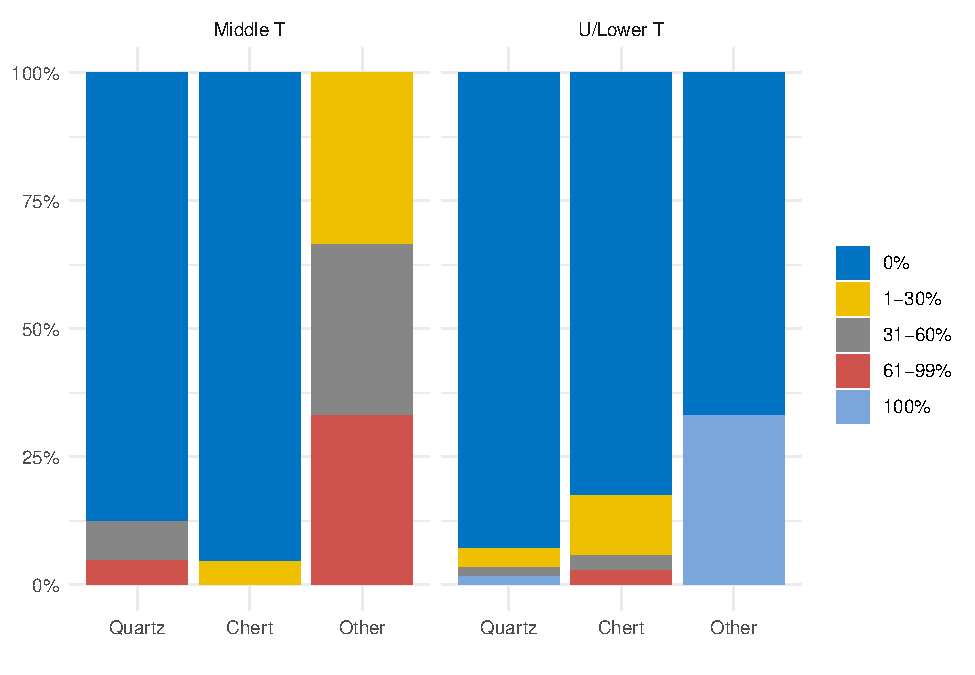
\includegraphics{thesis_files/figure-latex/cortexlp-1.pdf}
\begin{table}

\caption{\label{tab:cortextabtg}Cortex type and localization by raw material (U/Lower T).}
\centering
\resizebox{\linewidth}{!}{
\begin{tabular}[t]{>{\bfseries}llll}
\toprule
Cortex attributes & Quartz & Chert & Total\\
\midrule
CortexType, n (\%) &  &  & \\
Cobble & 3 (75.0) & 0 (0.0) & 5 (41.7)\\
Indeterminate & 1 (25.0) & 4 (66.7) & 5 (41.7)\\
Outcrop & 0 (0.0) & 2 (33.3) & 2 (16.7)\\
\bottomrule
\end{tabular}}
\end{table}
\begin{table}

\caption{\label{tab:cortextabpr}Cortex type and localization by raw material (Proto-Solutrean).}
\centering
\resizebox{\linewidth}{!}{
\begin{tabular}[t]{>{\bfseries}lllll}
\toprule
Cortex attributes & Quartz & Chert & Other & Total\\
\midrule
CortexType, n (\%) &  &  &  & \\
Cobble & 3 (100.0) & 0 (0.0) & 1 (50.0) & 4 (57.1)\\
Indeterminate & 0 (0.0) & 2 (100.0) & 1 (50.0) & 3 (42.9)\\
CortexLocation, n (\%) &  &  &  & \\
Distal & 2 (66.7) & 0 (0.0) & 0 (0.0) & 2 (28.6)\\
\addlinespace
Proximal & 0 (0.0) & 1 (50.0) & 1 (50.0) & 2 (28.6)\\
RightLateral & 1 (33.3) & 1 (50.0) & 1 (50.0) & 3 (42.9)\\
\bottomrule
\end{tabular}}
\end{table}
\hypertarget{technological-analysis}{%
\section{Technological analysis}\label{technological-analysis}}

\hypertarget{cores}{%
\subsection{Cores}\label{cores}}

\hypertarget{vale-boi-4}{%
\subsubsection{Vale Boi}\label{vale-boi-4}}

Cores are composed of a total of 123 pieces, with 46 total pieces on Lower 5, and 77 on Upper 5/4E.

Regarding their morphological types, and excluding inform cores, which were not considered here because they do not possess all the recordable attributes, there seems to be the preference for single platform types of core, for most raw materials, and through both phases. Chert, however, seems to have most variety of core types, although Lower 5 shows a preference for prismatic, while Upper 5/4E as relatively similar percentages between most types of cores. Cores appear mostly with 1 to 3 cores faces on both phases.

The cores seem to have been used mainly for the extraction of flakes, which, on both phases, have the biggest percentages on main face core use, although blade scars also have relatively high frequencies.

Most of the analysed core platforms are plain or cortical. On Upper 5/4E there is, however, a small frequency (3\% and 18.5\% respectively) of faceted platforms on quartz and chert. Platforms width and thickness means show smaller platforms for chert on both phases, while greywacke shows the biggest means for platform measurements.

This pattern is similar for core size, where chert and quartz exhibit the smaller means, although chert seems to have more elongated cores, on both phases, while greywacke and other raw materials have bigger dimensions.

Regarding elongation, figure X shows wider range and higher elongation values for chert cores in both phases, although Upper 5/4E seems to have less elongated cores, in both chert and quartz. Other raw materials, including greywacke, show the lower values for elongation. Chert for both phases and quartz on Upper 5/4E seem to be skewed bellow, showing less flake elongation variability when regarding low elongation ratios.

Regarding flattening (figure X), calculated by dividing maximum width by thickness, greywacke and other raw materials show higher flattening values, with quartz and chert showing similar values for both phases, with flattening median values of around 1.5, fairly centered in between the second and third quartil.
\begin{figure}
\centering
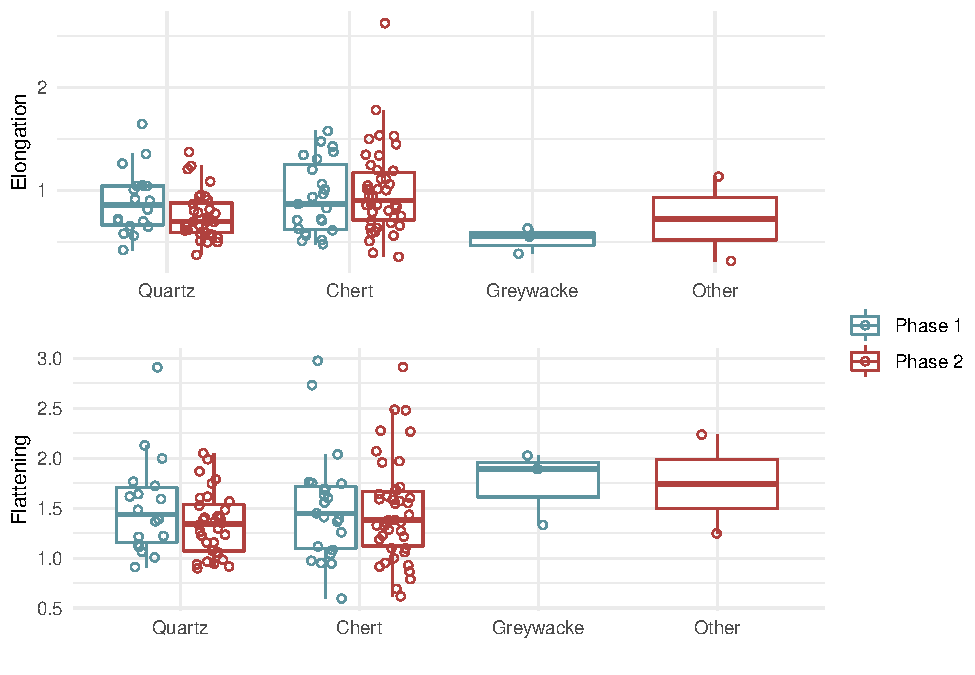
\includegraphics{thesis_files/figure-latex/corebloxplot-1.pdf}
\caption{\label{fig:corebloxplot}Core elongation and flattening boxplots by Phase.}
\end{figure}
\hypertarget{lapa-do-picareiro-4}{%
\subsubsection{Lapa do Picareiro}\label{lapa-do-picareiro-4}}

There are a total of 7 cores in the assemblage, 2 in the U/Lower T group and 5 in the Middle T, of which 2 are in chert and 2 in quartz.

Cores show a variability of types, ranging between single platform, prismatic and pyramidal for the Middle T group. These were mainly used to remove flakes, although on the Middle T group there are also frequent removals of mixed types of blanks. Platforms tend to be plain, although there is also the presence of dihedral platforms. Core faces seem to be in greater numbers on chert, for the Middle T group, with higher frequencies on 4 faces, while quartz varies between 1 face and 3.

In terms of measurements, chert seems to have the smallest means for core size, compared to others raw materials, showing, however, the highest elongation ratios (fig X). Regarding quartz cores, the differences between the U/Lower T phase and the Middle T phase are very obvious, with U/Lower T showing fairly more elongated cores with low flattening values, although these explicit differences may simply be the result of the small sample, which offered reduced internal assemblage variability.
\begin{figure}
\centering
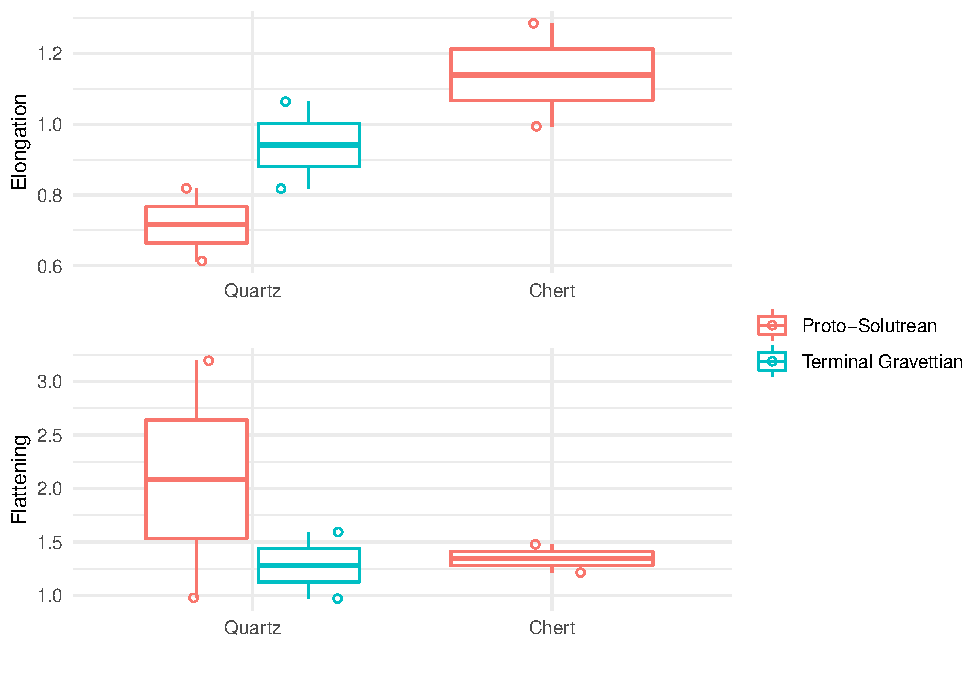
\includegraphics{thesis_files/figure-latex/corebloxplotLP-1.pdf}
\caption{\label{fig:corebloxplotLP}Core elongation and flattening boxplots by Phase.}
\end{figure}
\hypertarget{core-preparation-products}{%
\subsection{Core preparation products}\label{core-preparation-products}}

Core preparation products represent a small fraction of Vale Boi's total assemblage, with 1 in Lower 5 and 6 in Upper 5/4E.

Core preparation products are of two identified types, core fronts and core tablets (figure X), the individual of Lower 5 being a core tablet in quartz. For Upper 5/4E, however, most core preparation products are in chert (n=5) with one identified individual in quartz.
\begin{table}

\caption{\label{tab:coreprep}Core preparation products by raw material for Upper 5/4E.}
\centering
\resizebox{\linewidth}{!}{
\begin{tabular}[t]{>{\bfseries}lrrr}
\toprule
Core preparation product & Chert & Quartz & Total\\
\midrule
CoreFront & 3 & 0 & 3\\
CoreTablet & 2 & 1 & 3\\
Total & 5 & 1 & 6\\
\bottomrule
\end{tabular}}
\end{table}
\hypertarget{flakes}{%
\subsection{Flakes}\label{flakes}}

\hypertarget{vale-boi-5}{%
\subsubsection{Vale Boi}\label{vale-boi-5}}

Flakes are composed of a total of 1474 pieces, 509 of those belonging to Lower 5 group, and 965 in Upper 5/4E group, a growth in number (not positively correlated to sediment weight) already expected by the general intensity of occupation and material density observed in the latter phase . Although there are generally more Flakes in quartz, it is obvious the difference in ratios between these two raw materials, when comparing Lower 5 to Upper 5/4E results.
\begin{figure}
\centering
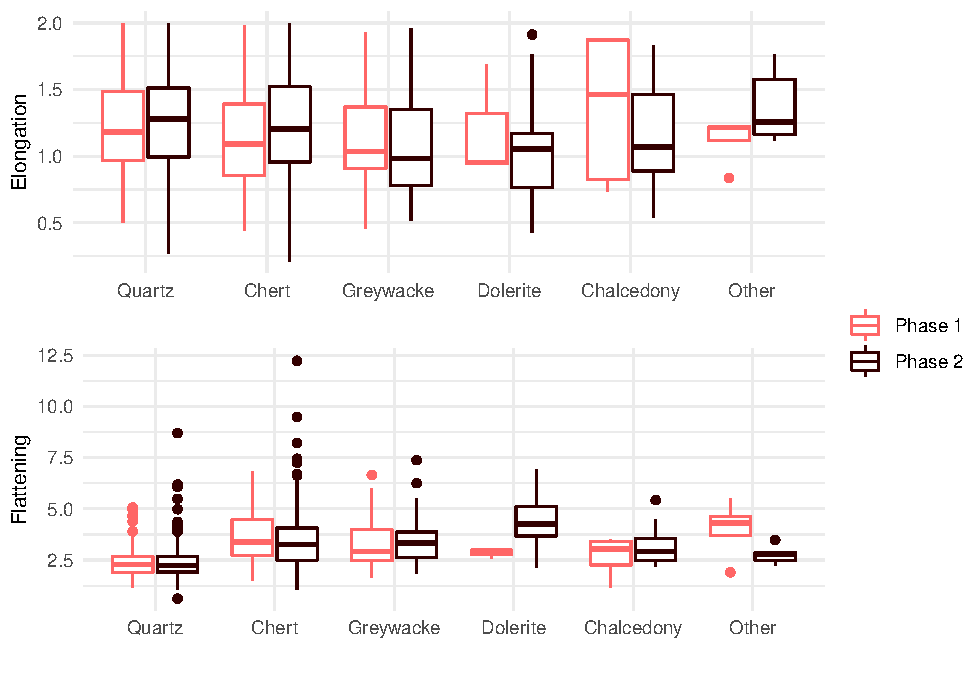
\includegraphics{thesis_files/figure-latex/flakeboxplot-1.pdf}
\caption{\label{fig:flakeboxplot}Flake elongation and flattening by phase and raw material.}
\end{figure}
Regarding morphology, for Lower 5 Flakes seem to have mostly irregular shapes, with frequencies over 45\% for most raw materials, followed by convergent and parallel shapes in lower frequencies (under 15\%). Dolerite, unlike other raw materials, shows only convergent and parallel shapes even if with low representativity (n=3). Cross sections are mostly irregular and triangular, varying slightly in frequency regarding each raw material, with straight and curved profiles, these two types of profiles representing each more than 40\% of chert Flakes. All raw materials, with exception of quartz, show high frequencies of straight profiles (over 40\%), chert showing a similar percentage between straight and curved profiles (44.3\% and 42.9\% respectively). Quartz, however, has a frequency of 65\% of straight profiles, showing much smaller frequencies for other types.

On Upper 5/4E, irregular shapes are still frequent, with frequencies over 25\% on all raw materials, although convergent and parallel shapes show higher frequencies (over 20\%) for quartz, chert and dolerite. Alike Lower 5, cross sections are mostly irregular (over 35\% for most raw materials) or triangular (over 25\% for all raw materials), and profile type show the same patterns and similar percentages as Lower 5.

Unidirectional scar patterns are dominant in both phases and all raw materials, with frequencies over 80\%. Bidirectional patterns are slightly more relevant in chert (9.3\%), and also in dolerite and chalcedony during Upper 5/4E. Dorsal patterns also show a dominance on both phases of 1, 2 and 3 scars for most raw materials, although chert shows the widest numbers and variety for higher scar counts.

Flakes have mostly plain platforms, although for certain raw materials, like quartz, there is a relevant presence of crushed platforms (33.3\% for Lower 5 and 35.9\% for Upper 5/4E). Faceted platforms are present in both phases but in low frequencies, in chert for both Lower 5 (1.4\%) and Upper 5/4E (2.4\%), but in no other raw material. Platforms also mostly non-cortical (between 80\% and 100\% depending on raw material) in both phases.

Blank metrics, including platform measurements, show for Lower 5, the smallest means in chalcedony and dolerite, followed by chert and quartz, where greywacke mean values show bigger Flakes in this raw material. On Upper 5/4E, however, the smallest Flakes are in chert, followed by quartz and chalcedony, where dolerite mean values are fairly closer to those of greywacke, thus making these the Flakes with highest metric mean values.

Regarding elongation, quartz, chert and chalcedony show the highest values, although the latter raw material shows a bigger concentration of similar elongation flakes in the third quartil, thus showing less general elongation. Despite having similar elongation ranges in both groups, quartz shows relatively different medians, on Lower 5 showing a less variability in the lower quartil, while Upper 5/4E shows lower variability in the upper quartil, hinting at a bigger number of consistently elongated quartz flakes in Upper 5/4E. For chert, Upper 5/4E also seems to show higher elongation values for flakes, though once again, there is a wide range of variability within regarding elongation in the assemblage.

As for flattening, quartz shows very low values for flake flattening, compared to other raw materials, although the data also shows the existance of a wide variability within each raw material, with the existance of several outliers which fall from the statistical groupings and quartils. As such, it seems that for all raw materials, perhaps with the exception of quartz, flake flattening is extremely variable in the assemblage.

\hypertarget{lapa-do-picareiro-5}{%
\subsubsection{Lapa do Picareiro}\label{lapa-do-picareiro-5}}

There are a total of plotted 122 Flakes, 46 attributed to the U/Lower T group, more than 50\% being in quartz, and 67 attributed to the Middle T group, its vast majority in chert. On both groups, attributes are very similar.

On the U/Lower T phase, for quartz, there seems to be the predominance of parallel shapes (36.8\%), followed by convergent ones (26.3\%). Chert, however, shows higher percentages for irregular (28.6\%) and divergent (42.9\%) shapes. Cross sections are mostly triangular for all raw materials (over 40\%), although chert also shows high frequencies of trapezoidal cross sections (42.9\%). Profiles are, for all raw materials, mostly straight (57.9\% on quartz and 85.7\% on chert) and terminations show relevant raw material differences, with quartz having bigger frequencies of feathered and hinged terminations (36.8\% both) and chert having a frequency of 42.9\% on pointed terminations. For all raw materials, there is the predominance of unidirectional dorsal patterns, high frequencies over 85\%. Dorsal scars show higher frequencies for 2 and 3 scars on quartz (36.8\% and 42.1\% respectively), while other raw materials show higher frequencies for 3 dorsal scars only (42.9\% on chert).

On the Middle T phase, quartz shows higher frequencies for irregular shapes (53.8\%), followed by convergent ones (38.5\%). Contrary to the patterns seen on the previous group, chert shows higher frequencies for parallel shapes (40.6\%). For all raw materials, cross sections are predominantly triangular (over 40\%) with straight profiles (over 50\%) and feathered terminations for chert (40.6\%), whereas quartz shows higher values for hinged terminations (46.2\%) followed by feathered (38.5\%). Alike the U/Lower T group, there is the predominance of unidirectional dorsal scar patterns (over 90\% for all raw materials), with high frequencies for 2 dorsal scars in quartz (61.5\%) and 2-3 dorsal scars in chert (34.4\% both).

Regarding platforms, for both groups, they are mostly plain for all raw materials (over 40\%), followed by relatively high values of crushed platforms in quartz, with the presence of 1 faceted platform for quartz and chert in each group. Chert on the Middle T group also shows dihedral platforms (18.8\%). Platforms seem to have barely any cortex, for all raw materials in both groups.

Measurements, including platform width and thickness, show larger means for the chert flakes (19.5 mm width and 27.3 mm length), comparatively to the quartz ones (16.7 mm width and 21.8 mm length), for Lower 5 and for Upper 5/4E (chert with 17.2 mm width and 20.9 mm length, and quartz with 13 mm width and 16.3 mm length). There also seems to be a size difference between groups, with the U/Lower T flakes showing bigger means (although with high standard deviation values), while Middle T means show smaller values and smaller SD values, the only constant seeming to be the thickness of flakes on chert (5-5.3 mm), wich seem to show little variability (standard deviations of 3.1 for the U/Lower T group and 2.3 for the Middle T group).
\begin{figure}
\centering
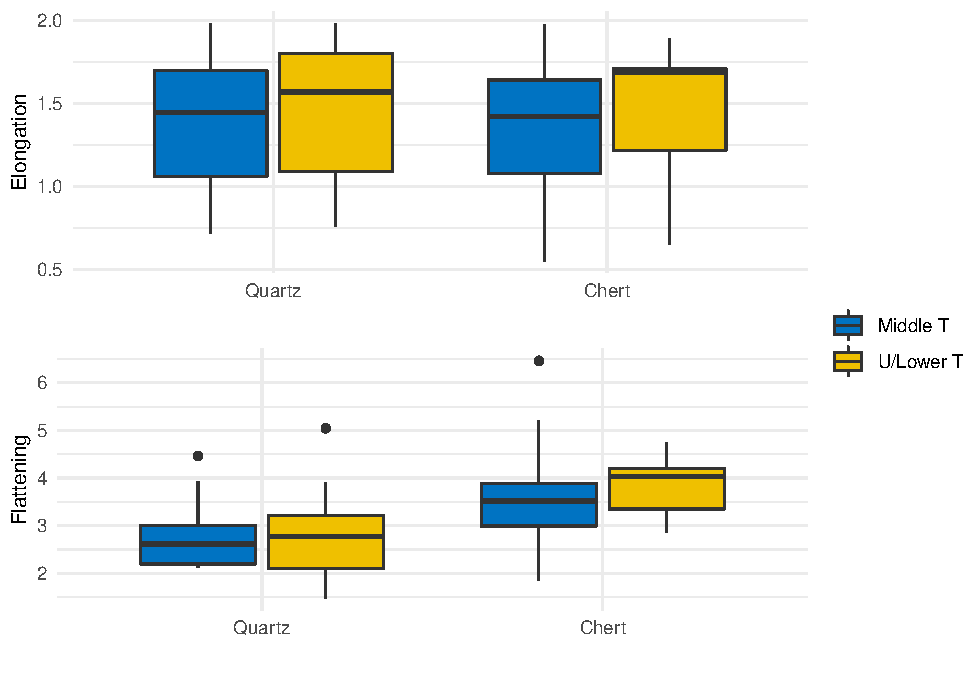
\includegraphics{thesis_files/figure-latex/flakeboxplotLP-1.pdf}
\caption{\label{fig:flakeboxplotLP}Flake elongation and flattening by phase and raw material.}
\end{figure}
Regarding elongation (figure X), values between quartz and chert and even between groups seem to be fairly similar, all with elongation ratios which seem skewed above, thus showing less elongation variability above the 1.5 threshold. Flake flattening, however, shows more apparent differences between raw materials, with quartz showing lower flattening ratios than chert. Within chert, however, there also seems to be a difference in general flattening variability and interquartil skewness, showing a larger number of flakes with similar flattening values (at around 4).

\hypertarget{elongated-blanks}{%
\subsection{Elongated blanks}\label{elongated-blanks}}

\hypertarget{vale-boi-6}{%
\subsubsection{Vale Boi}\label{vale-boi-6}}

There are a total of 219 elongated products in the assemblage (fig X), 82 of them being inserted in Lower 5, while 137 are inserted in Upper 5/4E. Comparatively to blanks, there seems to be a larger number of chert pieces (n=106), this number only changing in Lower 5, where quartz elongated blank numbers (n=44) supersede chert ones (n=31).

For both phases, however, elongated blank attributes are relatively similar, following the same general patterns.

Regarding morphology, elongated blanks have mostly parallel and convergent shapes, on both phases, although Lower 5 shows wider raw material differences, where 63.6\% of quartz has a parallel shapes whereas 51.6\% of chert has convergent ones. Cross sections are mostly triangular, with straight profiles, although there are also high frequencies for curved profiles.

Scar patterns show an obvious tendency for unidirectional knapping strategies on all raw materials. For Lower 5, however, there is the presence of bidirectional scar direction on chert even if in low frequencies (12.9\%), Upper 5/4E showing much lower values for this type of scar pattern, with 2\% on quartz and 4\% on chert. Scar count shows a tendency for 1 to 3 dorsal scars on both phases and all raw materials.

Elongated blanks on both phases seem to be obtained without platform preparation, since most platforms are plain, although quartz also shows crushed platforms. Only two faceted platforms were identified, in Upper 5/4E, on chert and dolerite. The general tendency for both phases is for the nonexistence of cortex on platforms, only certain raw materials showing complete cortical platforms, chert and greywacke on Lower 5 (9.7\% and 16.7\% respectively) and chert on Upper 5/4E (13.3\%).

Finally, elongated products metrics, including platform measurements, show a tendency on both phases for smaller blanks on quartz, followed by chert, where greywacke, dolerite and chalcedony show the biggest blanks and widest platforms. On both stages, means for width, length and thickness for quartz and chert are around 9mm, 21-26mm, 5mm respectively, with higher standard deviation values for length, which is what seems to vary most in these blanks. Despite this, chert elongated blanks seem to show means which hint for higher elongation ratios than quartz.

When plotting width and length for elongated products, by raw material, there seems to be separated groups, for both phases, instead of a continuous dispersion, which may indicate separate production strategies and/or desired dimensions for products.

For Lower 5 there seems to be the existence of one single group for quartz, and two differing groups of width-length combinations for chert (Fig X), although the sample is small, possibly having an impact on the data dispersion. As such, this group in quartz might suggest the preference in Lower 5 for the production of small elongated blanks between 3-10 mm width and under 25 mm length, easily understood by the density curves. This group falls into the definition of bladelet, for the exception of a small quantity of pieces from the latter group, which, due to their width surpassing 12 mm width, are considered blades. Regarding chert, measurements are slightly more dispersed, allowing for the individualization of a wide group of smaller blanks, ranging between 2.5-12 mm width, peaking at around 10 mm, and 10-28 mm length peaking at around 20 mm, again mostly falling into the traditional definition of bladelets. The interpretation of the second group is further truncated by the small sample. The curves show not an increase in density, but instead a maintenance of the curve after a moment of drop, which might not represent a preference. Elongated products in this group have widths and lengths comprehended between 14-17 mm and 30-40 mm respectively, and can be classified as blades.

For Upper 5/4E, quartz continues to have a small sample that seems to show disperse concentrations of products, with a first group of small blanks between 2.5-6 mm width and under 20 mm length, and a second group ranging between 10-12.5 mm width and 20-30 mm length, both classified as bladelets. For quartz, there seems to be a wider dispersion without an obvious peak in the density curve, even within the two groups. For chert, there are three visible concentrations of elongated blanks, although with varying sample numbers on each group: one small group ranging between 2.5-5 mm width and 10-20 mm width, classifying as bladelets; an intermediate group and the best represented in terms of sample numbers, between 8-12.5 mm width and 15-30 mm length, classifying as bladelets with the exception of 2 pieces with slightly exceed the width bladelet limit; a group of larger blanks, with a small sample, ranging between 13-16 mm width and 30-42 mm length, traditionally classified as blades. Regarding the density curves, however, chert seems to peak between 7.5-10 mm width and 20 mm length, showing instead a unimodal curve and possibly, only one prefered width/length ratio with a wider dispersion.
\begin{figure}
\centering
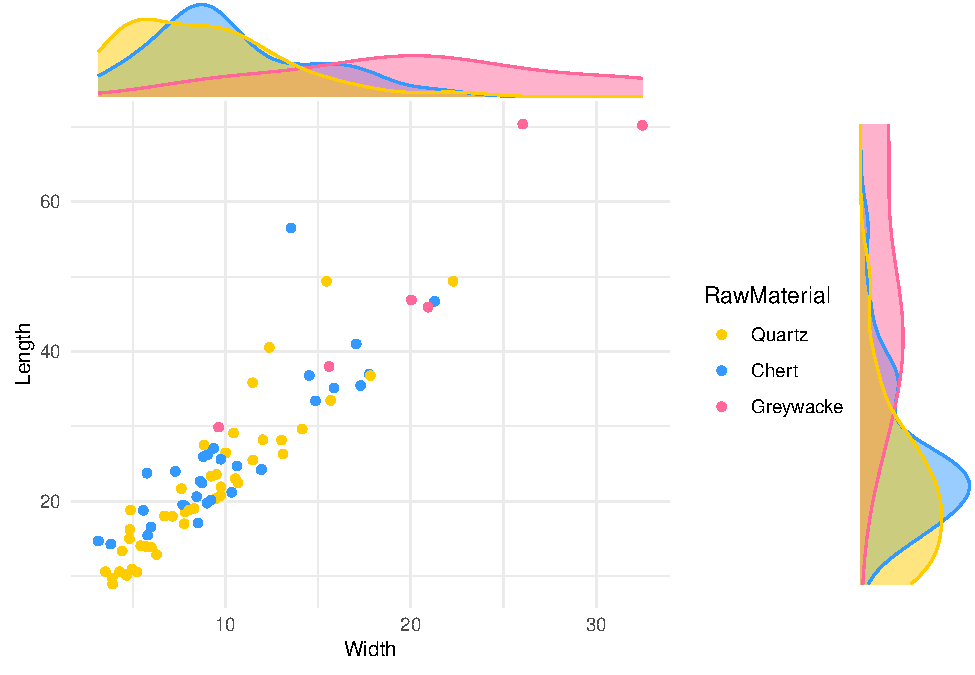
\includegraphics{thesis_files/figure-latex/elongdisp1-1.pdf}
\caption{\label{fig:elongdisp1}Elongated product width and length dispersion by raw material (Lower 5).}
\end{figure}
\begin{figure}
\centering
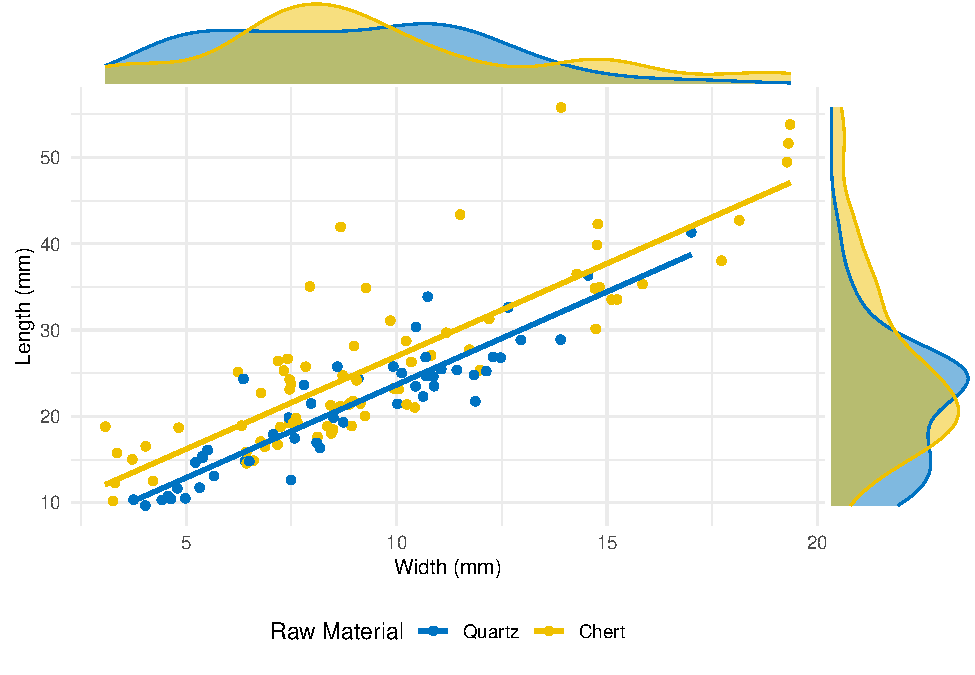
\includegraphics{thesis_files/figure-latex/elongdisp2-1.pdf}
\caption{\label{fig:elongdisp2}Elongated product width and length dispersion by raw material (Upper 5/4E).}
\end{figure}
\hypertarget{lapa-do-picareiro-6}{%
\subsubsection{Lapa do Picareiro}\label{lapa-do-picareiro-6}}

There are a total of plotted 47 elongated blanks, 27 of which belong to the U/Lower T group, more than 50\% on chert, and 20 to the Middle T group, also more than 50\% on chert.

Technological attributes follow closely those already described in blanks, also showing little variation between the U/Lower T and the Middle T.

Elongated blanks show a majority of parallel shapes, followed by convergent, with triangular cross sections, straight profiles followed by curved, with the exception of quartz on the Middle T group, where curved profiles are more frequent. Dorsal scars are unidirectional, with 2 negatives for quartz and 2 to 4 negatives for chert.

Platforms are mostly plain, with no cortex, where quartz seems to have the smaller dimensions.

When plotting width and length for elongated blanks, for chert and quartz, there seems to be two groups of differing dimensions. Regarding the U/Lower T, there is a group of smaller blanks, ranging between 2-10 mm of width and 5-25 mm of length, thus falling into the traditional category of bladelet, and a larger group, although much more disperse and composed mostly of chert, with widths and length ranging between 13-26 mm and 40-60 mm respectively, which may be classified as blades. The density curves for width and length on chert, however, don't seem to show the relevant existance of two groups, with only a continuous increase in values within each variables.

For the Middle T there is also a group of smaller blanks, with width ranging the 3-10 mm width, although length values vary a lot more, going between the 5-30 mm, where the higher values are made up mostly of chert. Even so, this group may be characterized through the traditional classification of bladelet. The second group is made up entirely of chert, although it has less blanks and is very disperse in terms of width, which is higher than 15 mm, and length, higher than 45 mm, also being characterized as blades. Once again, for chert, density curves seem to show a unimodal curve.

These patterns may represent differing production strategies for specific elongated blank sizes and ratios, although, given the altitude of the site, it might simply reflect the truncated reduction sequences present at the site, thus only showing the presence of two wide groups of small elongated blanks and larger elongated blanks. without the intermediate group which wasn't transported into the site.
\begin{figure}
\centering
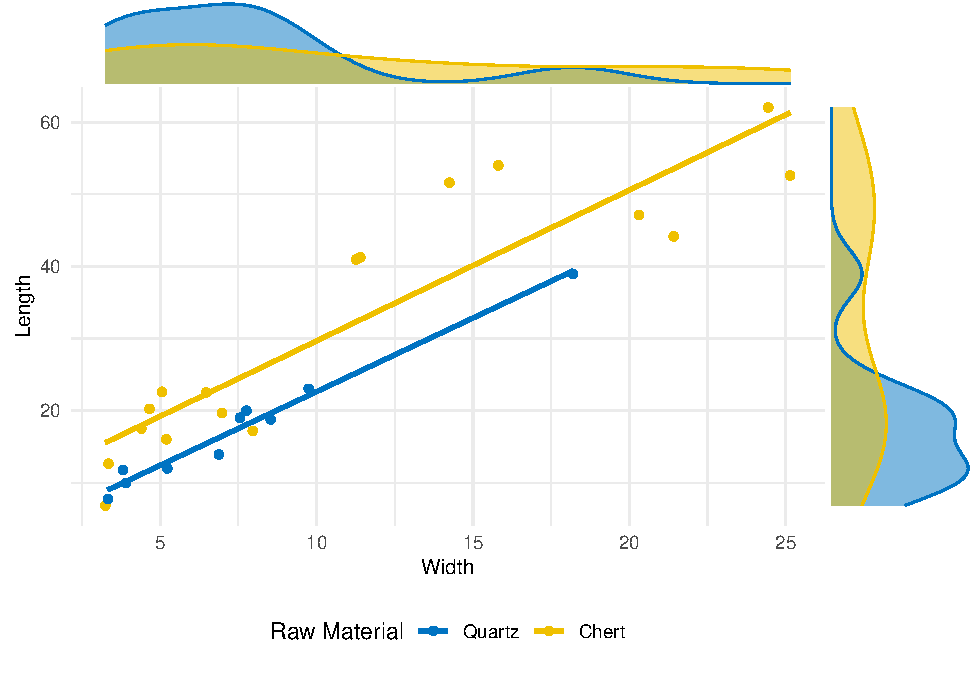
\includegraphics{thesis_files/figure-latex/elongdisp1LP-1.pdf}
\caption{\label{fig:elongdisp1LP}Elongated product width and length dispersion by raw material (U/Lower T).}
\end{figure}
\begin{figure}
\centering
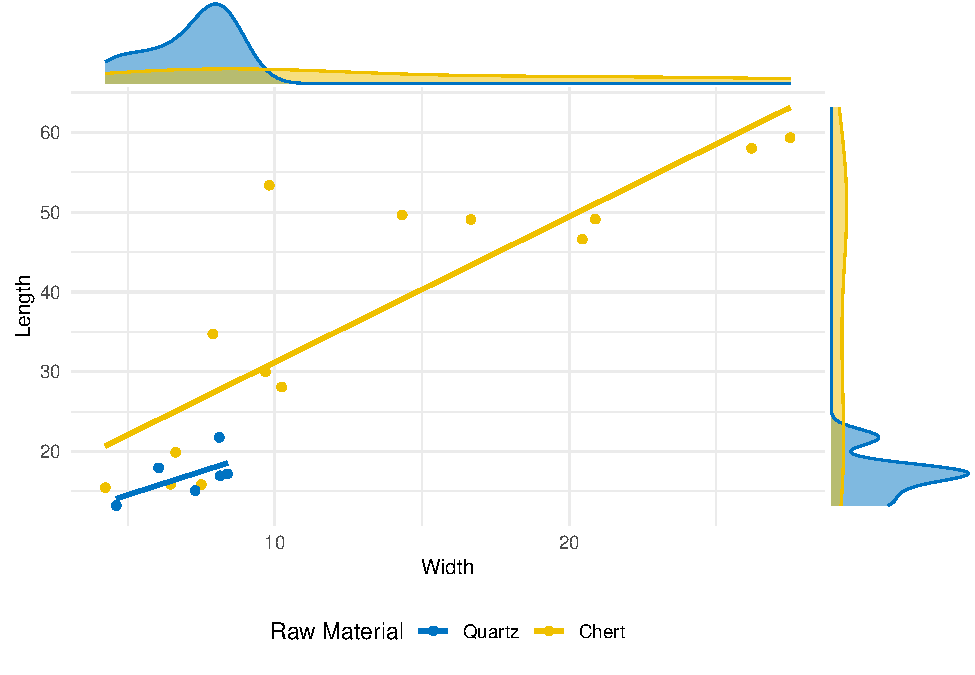
\includegraphics{thesis_files/figure-latex/elongdisp2LP-1.pdf}
\caption{\label{fig:elongdisp2LP}Elongated product width and length dispersion by raw material (Middle T).}
\end{figure}
\hypertarget{retouched-tools}{%
\subsection{Retouched tools}\label{retouched-tools}}

\hypertarget{vale-boi-7}{%
\subsubsection{Vale Boi}\label{vale-boi-7}}

As seen before, retouched pieces make up a small percentage of the assemblage, with 167 identified pieces, from which 55 can be inserted in the Lower 5 group (fig X), while 112 in the Upper 5/4E group (fig X).

Lower 5 is comprised of several typologies, from which a few stand out by their high numbers, such as retouched flakes, corresponding to 27\% of total retouched pieces, mostly in chert, splintered pieces, with 25.4\% of representativity, followed by notches with a frequency of 12.7\%, both occurring in similar numbers in chert (n=6 and n=4 respectively) and quartz (n=8 and n=3).
There is also the presence of endscrapers (9.09\%) and burins (7.27\%), mostly on chert, although their frequencies in the total of retouched pieces isn't very representative.

For Upper 5/4E, splintered pieces are still very frequent (24.1\%), in both chert and quartz, followed by endscrapers which represent 22.3\% of the total retouched piece number, most of them in chert, although it may be relevant to point out 2 are made of dolerite. Notches are, once again, the third most frequent retouched typology, with 11.6\% representativity, though most are found in quartz. Every other typology has frequencies under 10\%.

Upper 5/4E thus shows not only a larger number of retouched pieces, which might be the result of a bigger occupation intensity, but also a wider variety of typologies. As Lower 5 shows 11 different retouched piece types, Upper 5/4E shows 16 types, introducing 6 new different typologies, as the double backed blade of stage 1 doesn't appear in the upper occupation.

One of these newly introduced retouched type is the Vale Comprido point, although only representing 5.3\% of retouched piece total for Upper 5/4E. As mentioned before, Vale Comprido points have been identified as a Proto-Solutrean only technological solution, which may appear during the Proto-Solutrean in the Two-phase model, or during either the Terminal Gravettian or Proto-Solutrean in the Three-phase model. Thus, its presence in Upper 5/4E not only conforms to the data already presented for the Portuguese Estremadura (Zilhão 1997) it further strengths the separation of layers 4E and 5 in two moments of differing occupation.

The analysed Vale Comprido points have been identified in chert (n=1), greywacke (n=1), dolerite (n=3) and chalcedony (n=1, which makes up 100\% of retouched pieces made in this raw material). In fact, dolerite had already been identified as a preferred means for making these products (Marreiros 2009), a fact only strengthened by the fact this raw material has more Vale Comprido points than any other, and only appears in one other typology, the endscraper. Comparatively, dolerite doesn't seem to be used for the production of any retouched piece in stage 1. These shall be described into further detail in Chapter 7.4.6.
\begin{landscape}\begin{table}[!h]

\caption{\label{tab:retouchphase1}Lower 5 retouched piece typology by raw material.}
\centering
\resizebox{\linewidth}{!}{
\begin{tabular}[t]{lrlrlrlrlrl}
\toprule
\multicolumn{1}{c}{\textbf{Typology}} & \multicolumn{1}{c}{\textbf{Quartz (n)}} & \multicolumn{1}{c}{\textbf{Quartz (\%)}} & \multicolumn{1}{c}{\textbf{Chert (n)}} & \multicolumn{1}{c}{\textbf{Chert (\%)}} & \multicolumn{1}{c}{\textbf{Greywacke (n)}} & \multicolumn{1}{c}{\textbf{Greywacke (\%)}} & \multicolumn{1}{c}{\textbf{Chalcedony (n)}} & \multicolumn{1}{c}{\textbf{Chalcedony (\%)}} & \multicolumn{1}{c}{\textbf{Total}} & \multicolumn{1}{c}{\textbf{Total (\%)}}\\
\midrule
Endscraper & 0 & 0\% & 4 & 10.53\% & 0 & 0\% & 1 & 100\% & 5 & 9.09\%\\
Dihedral Burin & 1 & 6.67\% & 3 & 7.89\% & 0 & 0\% & 0 & 0\% & 4 & 7.27\%\\
Burin on truncation & 0 & 0\% & 2 & 5.26\% & 0 & 0\% & 0 & 0\% & 2 & 3.64\%\\
Truncation & 0 & 0\% & 1 & 2.63\% & 0 & 0\% & 0 & 0\% & 1 & 1.82\%\\
Notch & 3 & 20\% & 4 & 10.53\% & 0 & 0\% & 0 & 0\% & 7 & 12.73\%\\
\addlinespace
Denticulate & 0 & 0\% & 2 & 5.26\% & 0 & 0\% & 0 & 0\% & 2 & 3.64\%\\
Splintered piece & 8 & 53.33\% & 6 & 15.79\% & 0 & 0\% & 0 & 0\% & 14 & 25.45\%\\
Double backed bladelet & 0 & 0\% & 2 & 5.26\% & 0 & 0\% & 0 & 0\% & 2 & 3.64\%\\
Retouched blade & 0 & 0\% & 1 & 2.63\% & 0 & 0\% & 0 & 0\% & 1 & 1.82\%\\
Retouched bladelet & 0 & 0\% & 2 & 5.26\% & 0 & 0\% & 0 & 0\% & 2 & 3.64\%\\
\addlinespace
Retouched flake & 3 & 20\% & 11 & 28.95\% & 1 & 100\% & 0 & 0\% & 15 & 27.27\%\\
Total & 15 & 100\% & 38 & 100\% & 1 & 100\% & 1 & 100\% & 55 & 100\%\\
\bottomrule
\end{tabular}}
\end{table}
\end{landscape}
\begin{landscape}\begin{table}[!h]

\caption{\label{tab:retouchphase2}Upper 5/4E Retouched piece typology by raw material.}
\centering
\resizebox{\linewidth}{!}{
\begin{tabular}[t]{lrlrlrlrlrlrl}
\toprule
\multicolumn{1}{c}{\textbf{Typology}} & \multicolumn{1}{c}{\textbf{Quartz (n)}} & \multicolumn{1}{c}{\textbf{Quartz (\%)}} & \multicolumn{1}{c}{\textbf{Chert (n)}} & \multicolumn{1}{c}{\textbf{Chert (\%)}} & \multicolumn{1}{c}{\textbf{Greywacke (n)}} & \multicolumn{1}{c}{\textbf{Greywacke (\%)}} & \multicolumn{1}{c}{\textbf{Dolerite (n)}} & \multicolumn{1}{c}{\textbf{Dolerite (\%)}} & \multicolumn{1}{c}{\textbf{Chalcedony (n)}} & \multicolumn{1}{c}{\textbf{Chalcedony (\%)}} & \multicolumn{1}{c}{\textbf{Total}} & \multicolumn{1}{c}{\textbf{Total (\%)}}\\
\midrule
Endscraper & 2 & 5.88\% & 21 & 30\% & 0 & 0\% & 2 & 40\% & 0 & 0\% & 25 & 22.32\%\\
Carinated endscraper & 0 & 0\% & 2 & 2.86\% & 1 & 50\% & 0 & 0\% & 0 & 0\% & 3 & 2.68\%\\
Perforator-endscraper & 0 & 0\% & 1 & 1.43\% & 0 & 0\% & 0 & 0\% & 0 & 0\% & 1 & 0.89\%\\
Perforator & 0 & 0\% & 1 & 1.43\% & 0 & 0\% & 0 & 0\% & 0 & 0\% & 1 & 0.89\%\\
Dihedral Burin & 2 & 5.88\% & 4 & 5.71\% & 0 & 0\% & 0 & 0\% & 0 & 0\% & 6 & 5.36\%\\
\addlinespace
Burin on truncation & 0 & 0\% & 4 & 5.71\% & 0 & 0\% & 0 & 0\% & 0 & 0\% & 4 & 3.57\%\\
Truncation & 0 & 0\% & 4 & 5.71\% & 0 & 0\% & 0 & 0\% & 0 & 0\% & 4 & 3.57\%\\
Notch & 10 & 29.41\% & 3 & 4.29\% & 0 & 0\% & 0 & 0\% & 0 & 0\% & 13 & 11.61\%\\
Denticulate & 1 & 2.94\% & 2 & 2.86\% & 0 & 0\% & 0 & 0\% & 0 & 0\% & 3 & 2.68\%\\
Splintered piece & 15 & 44.12\% & 12 & 17.14\% & 0 & 0\% & 0 & 0\% & 0 & 0\% & 27 & 24.11\%\\
\addlinespace
Backed bladelet & 0 & 0\% & 1 & 1.43\% & 0 & 0\% & 0 & 0\% & 0 & 0\% & 1 & 0.89\%\\
Backed bladelet parcial & 0 & 0\% & 1 & 1.43\% & 0 & 0\% & 0 & 0\% & 0 & 0\% & 1 & 0.89\%\\
Retouched blade & 0 & 0\% & 2 & 2.86\% & 0 & 0\% & 0 & 0\% & 0 & 0\% & 2 & 1.79\%\\
Retouched bladelet & 0 & 0\% & 5 & 7.14\% & 0 & 0\% & 0 & 0\% & 0 & 0\% & 5 & 4.46\%\\
Retouched flake & 4 & 11.76\% & 6 & 8.57\% & 0 & 0\% & 0 & 0\% & 0 & 0\% & 10 & 8.93\%\\
\addlinespace
Total & 34 & 100\% & 70 & 100\% & 2 & 100\% & 5 & 100\% & 1 & 100\% & 112 & 100\%\\
\bottomrule
\end{tabular}}
\end{table}
\end{landscape}
\hypertarget{lapa-do-picareiro-7}{%
\subsubsection{Lapa do Picareiro}\label{lapa-do-picareiro-7}}

The total number of retouched pieces which have spatial information, allowing the identification of phase is 11, of which 6 belong to the U/Lower T group and 5 on the Middle T.

As seen on table X, the U/Lower T shows 4 types of retouched piece typologies, the most present being the retouched flakes (of varied elongation ratios, n=3) all in chert, where the only quartz retouched piece is a splintered piece. From the retouched flakes, one shows similarities with the Vale Comprido point, although the platform/dorsal retouched as to thin the platform is questionable.

For the Middle T group (table x), there is a smaller variety of retouched pieces, all in chert: a notch, retouched flakes (n=2), a truncation and possibly a Vale Comprido point.
\begin{table}[!h]

\caption{\label{tab:retouchTG}U/Lower T retouched piece typology by raw material.}
\centering
\resizebox{\linewidth}{!}{
\begin{tabular}[t]{lrlrlrl}
\toprule
\multicolumn{1}{c}{\textbf{Typology}} & \multicolumn{1}{c}{\textbf{Quartz (n)}} & \multicolumn{1}{c}{\textbf{Quartz (\%)}} & \multicolumn{1}{c}{\textbf{Chert (n)}} & \multicolumn{1}{c}{\textbf{Chert (\%)}} & \multicolumn{1}{c}{\textbf{Total}} & \multicolumn{1}{c}{\textbf{Total (\%)}}\\
\midrule
Dihedral angle burin & 0 & 0\% & 1 & 20\% & 1 & 16.67\%\\
Notch & 0 & 0\% & 1 & 20\% & 1 & 16.67\%\\
Splintered piece & 1 & 100\% & 0 & 0\% & 1 & 16.67\%\\
Retouched flake & 0 & 0\% & 3 & 60\% & 3 & 50\%\\
\bottomrule
\end{tabular}}
\end{table}
\begin{table}[!h]

\caption{\label{tab:retouchPR}Upper 5/4E Retouched piece typology by raw material.}
\centering
\resizebox{\linewidth}{!}{
\begin{tabular}[t]{lrlr}
\toprule
\multicolumn{1}{c}{\textbf{Typology}} & \multicolumn{1}{c}{\textbf{Chert (n)}} & \multicolumn{1}{c}{\textbf{Chert (\%)}} & \multicolumn{1}{c}{\textbf{Total}}\\
\midrule
Concave truncation & 1 & 20\% & 1\\
Vale Comprido point (?) & 1 & 20\% & 1\\
Notch & 1 & 20\% & 1\\
Retouched flake & 2 & 40\% & 2\\
\bottomrule
\end{tabular}}
\end{table}
The analysis of retouched pieces at Lapa do Picareiro is, however, possibly truncated by the edge damage of the assemblage. In all levels, many pieces, both quartz and chert, although in wider quantities in the latter, show variable degrees of edge damage, from light to extensive. Although some edges were obviously damaged by, either trampling or impact by blocks, since there was no homogeneity in its distribution or directionality, some other edges show dubious marks. As such, the present study opted for a more reserved approach regarding the classification of retouch, understanding the caveats of the decision. Thus, retouched pieces, specially the retouched flakes, were only identified as such whenever they displayed homogeneous, localized and unidirectional retouch, which could not be mistaken for edge damage.

\hypertarget{vale-comprido-technology}{%
\subsection{Vale Comprido technology}\label{vale-comprido-technology}}
\begin{figure}
\centering
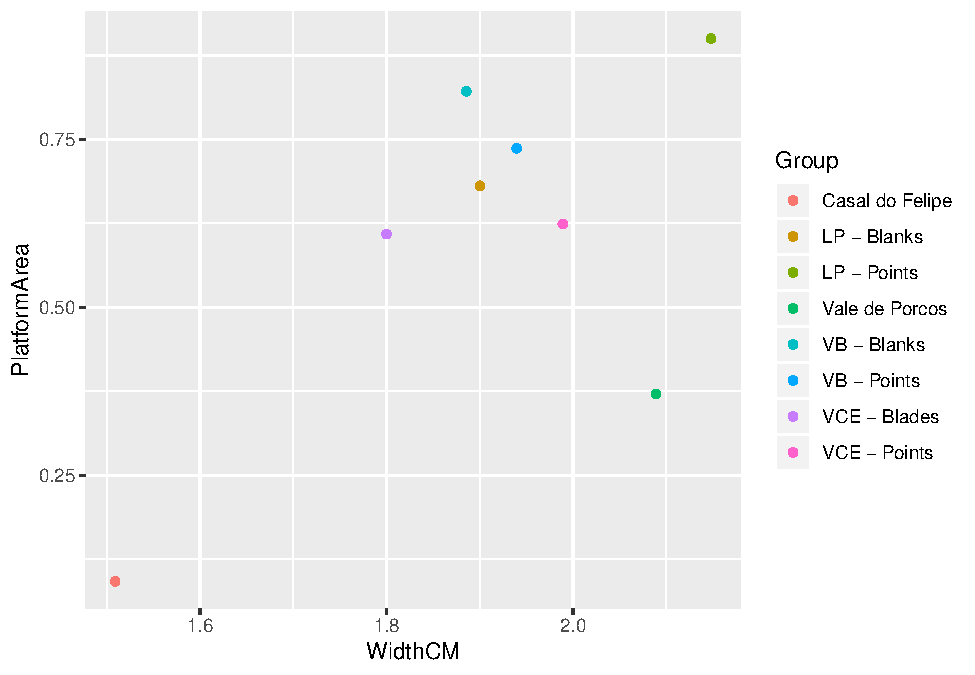
\includegraphics{thesis_files/figure-latex/vca-1.pdf}
\caption{\label{fig:vca}Blank width and platform area of Vale Comprido points and blanks from Vale Boi, Lapa do Picareiro (present analysis) and Casal do Felipe, Vale de Porcos and Vale Comprido - Encosta (Zilhão and Aubry 1995).}
\end{figure}
\begin{figure}
\centering
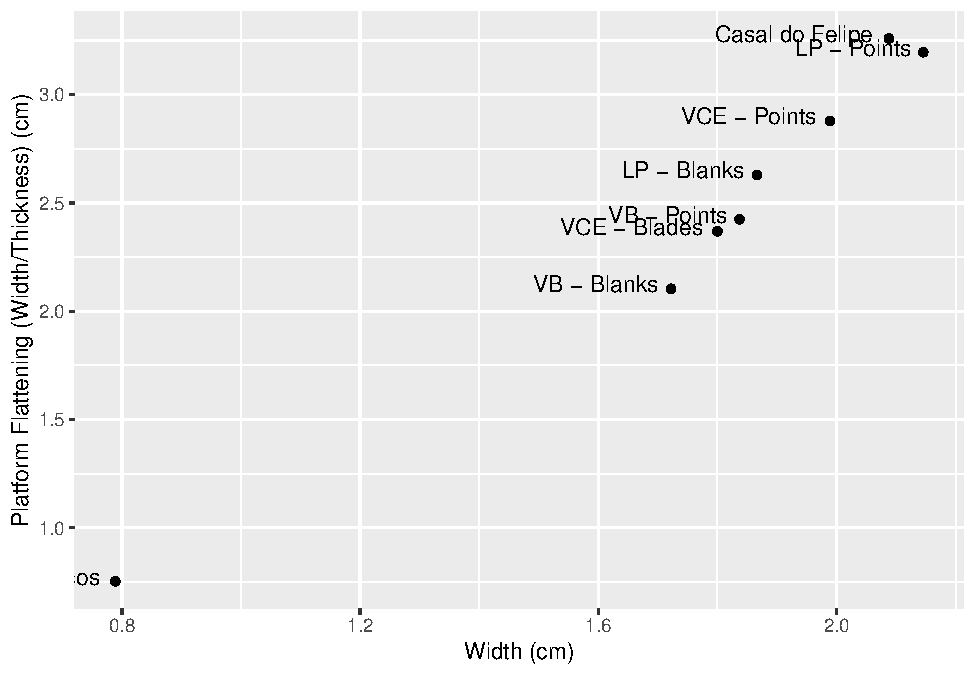
\includegraphics{thesis_files/figure-latex/vcb-1.pdf}
\caption{\label{fig:vcb}Blank width and platform convexity of Vale Comprido points and blanks from Vale Boi, Lapa do Picareiro (present analysis) and Casal do Felipe, Vale de Porcos and Vale Comprido - Encosta (Zilhão and Aubry 1995)}
\end{figure}
\begin{figure}
\centering
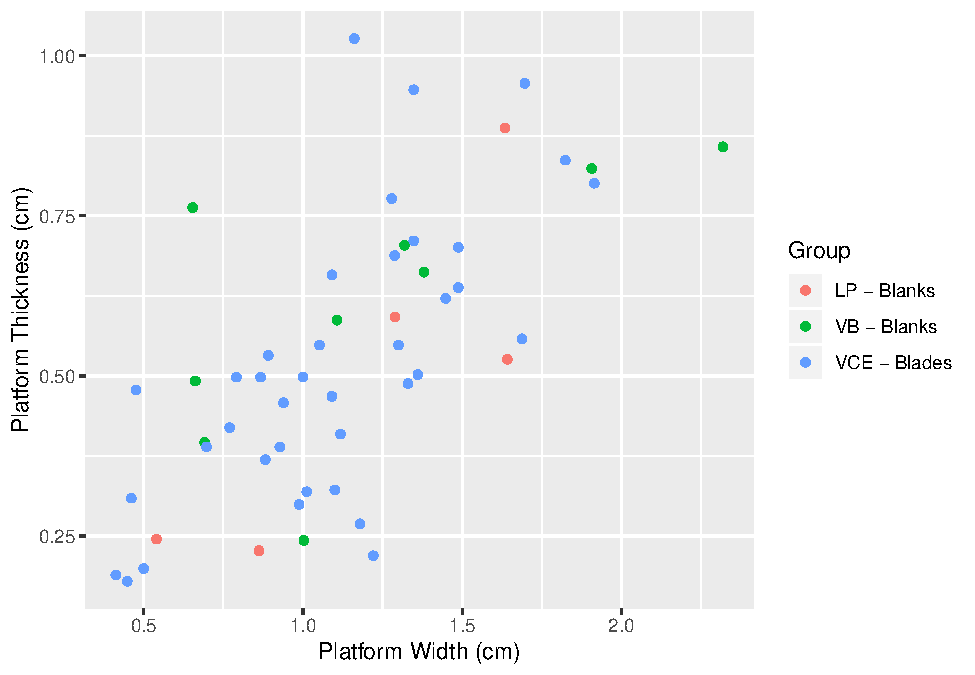
\includegraphics{thesis_files/figure-latex/vcc-1.pdf}
\caption{\label{fig:vcc}Platform width and thickness of Vale Comprido points and blanks from Vale Boi, Lapa do Picareiro (present analysis) and Vale Comprido - Encosta (Zilhão and Aubry 1995).}
\end{figure}
\hypertarget{multivariate-analysis}{%
\subsection{Multivariate analysis}\label{multivariate-analysis}}

\hypertarget{vale-boi-8}{%
\subsubsection{Vale Boi}\label{vale-boi-8}}

Core morphology is aimed to understand core form, reduction intensity and raw material quality and shape (Scerri et al.~2014).

The two dimensions in figure X explain 60.8\% of total sample variance, where dimension 1 explains 33.1\% and dimension 2 explains 27.7\%. A summary of these dimensions, variables in each axis and description/interpretation may be found on table X.

Dimension 1 is represented by flatter cores with larger weight values in the positive loadings, negatively correlated to core elongation on the negative loadings. This means that bigger cores (using weight as a proxy for size) tend to be less elongated, and as the core loses its mass, shapes tend to elongate. This dimension seems to gain its statistical relevance from a group of weight driven variations, though this may be caused by a small number of high values.

Dimension 2 shows an inverse correlation between weight, on the negative loadings (although seemingly not very pronounced) with core elongation, convergence and flattening, that, on the positive loadings, seem to correlate positively. This might represent the reduction of total core volume and subsequential core shapping (Scerri et al.~2014).

Regarding phases, the assemblage from Upper 5/4E seems concentrated on the negative loadings of dimension 2, which might represent the assemblage is driven by morphological changes, between cores that are more elongated, convergent and flatter and some that are less elongated (Scerri et al.~2014). Despite this, core morphology variation between groups seems similar, although Lower 5 does show more weight driven variation than Upper 5/4E.
\begin{figure}
\centering
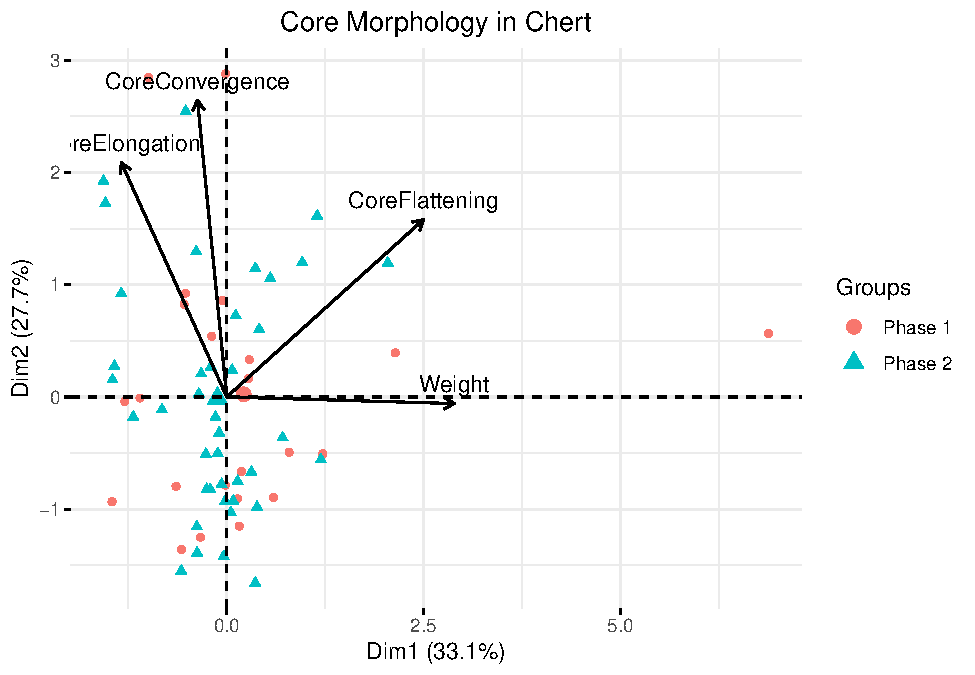
\includegraphics{thesis_files/figure-latex/unnamed-chunk-12-1.pdf}
\caption{\label{fig:unnamed-chunk-12}Variable plot of the first and second components of the Core Morphology PCA on chert (CMC).}
\end{figure}
\begin{table}[!h]

\caption{\label{tab:unnamed-chunk-13}Positive and negative principal component scores, Core Morphology PCA (CMC).}
\centering
\begin{tabular}[t]{lc>{\raggedright\arraybackslash}p{3cm}>{\raggedright\arraybackslash}p{3cm}>{\raggedright\arraybackslash}p{3cm}}
\toprule
\multicolumn{1}{c}{\textbf{Dimensions}} & \multicolumn{1}{c}{\textbf{\% variability}} & \multicolumn{1}{>{\centering\arraybackslash}p{3cm}}{\textbf{+}} & \multicolumn{1}{>{\centering\arraybackslash}p{3cm}}{\textbf{-}} & \multicolumn{1}{>{\centering\arraybackslash}p{3cm}}{\textbf{Interpretation}}\\
\midrule
1 & 33.1\% & Core flattening, Weight & Core convergence, Core elongation & Tendency for flatter cores to be elongated, more convergent and heavier.\\
2 & 27.7\% & Core convergence, Core flattening, Core elongation &  & Flatter cores associated with highter elongation racios and convergence. As these characteristics increase, weight reduces.\\
Cumulative \% & 60.8\% &  &  & \\
\bottomrule
\end{tabular}
\end{table}
The two dimensions from core morphology in quartz (CMQ) explain 62.3\% of sample variance.

Dimension 1, representing 32.9\% of variance, shows on the positive loadings flatter and more convergent values, inversely correlated with core elongation, meaning that as cores become flatter and with higher values of convergence, they become less elongated.

Dimension 2, explaining 29.4\% of variance, is dominated by the inverse correlation between weight (on the negative loadings) with core elongations, convergence and flattening (on the positive loadings), once again repeating the pattern already observed on chert, and which might represent the reduction of core volume through knapping.

Lower 5 is mostly represented on the positive loadings of dimension 2, meaning it is dominated by high scores in core elongation, convergence and flattening, while Upper 5/4E seems to be mostly located on the negative loadings. This might mean that cores in Lower 5 might be more elongated and smaller, with a variation better explained by morphology, whereas core variation from Upper 5/4E might be better explained by changes in mass than changes in convergence or flattening, although there seems to be some tendency for elongated cores in Upper 5/4E as well.
\begin{figure}
\centering
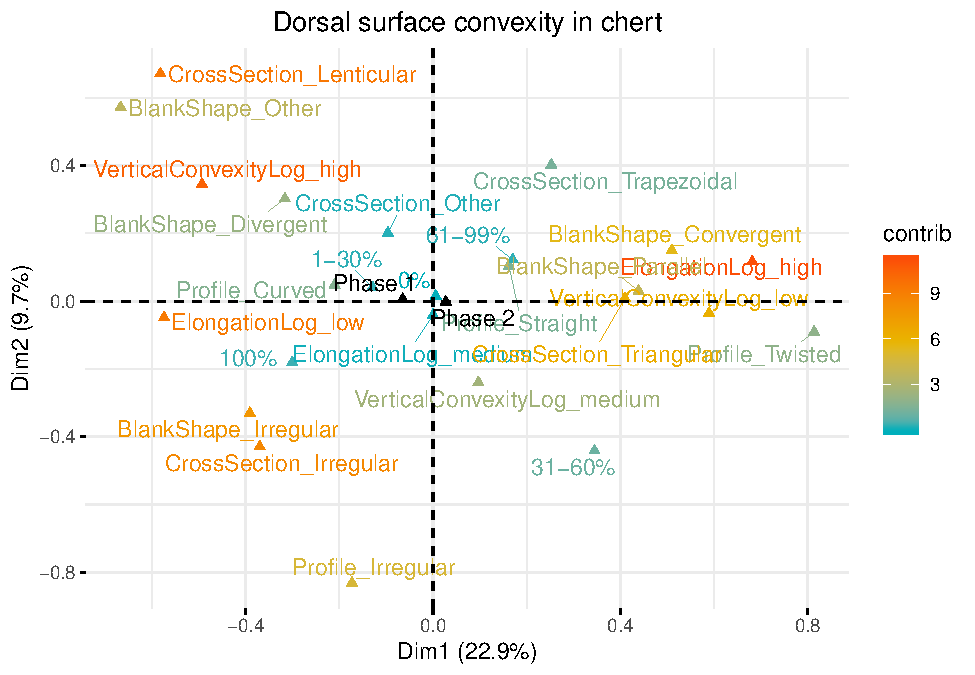
\includegraphics{thesis_files/figure-latex/unnamed-chunk-14-1.pdf}
\caption{\label{fig:unnamed-chunk-14}Variable plot of the first and second components of the Core Morphology PCA on quartz (CMQ).}
\end{figure}
\begin{table}[!h]

\caption{\label{tab:unnamed-chunk-15}Positive and negative principal component scores, Core Morphology PCA (CMQ).}
\centering
\begin{tabular}[t]{lc>{\raggedright\arraybackslash}p{3cm}>{\raggedright\arraybackslash}p{3cm}>{\raggedright\arraybackslash}p{3cm}}
\toprule
\multicolumn{1}{c}{\textbf{Dimensions}} & \multicolumn{1}{c}{\textbf{\% variability}} & \multicolumn{1}{>{\centering\arraybackslash}p{3cm}}{\textbf{+}} & \multicolumn{1}{>{\centering\arraybackslash}p{3cm}}{\textbf{-}} & \multicolumn{1}{>{\centering\arraybackslash}p{3cm}}{\textbf{Interpretation}}\\
\midrule
1 & 32.9\% & Core flattening, Core convergence & Core elongation & Tendency for flatter cores to be elongated and convergent.\\
2 & 29.4\% & Core elongation, Core flattening, Core convergence & Weight & Flatter cores associated with highter elongation racios and convergence. As these characteristics increase, weight reduces.\\
Cumulative \% & 62.3\% &  &  & \\
\bottomrule
\end{tabular}
\end{table}
Core use domain aims to understand how knappers reduced cores using different techniques to shape them (Scerri et al.~2014). The first two components in the chert core use analysis explain a cumulative percentage of 53.5\% of the assemblage's variability.

Dimension one (table X) explains 29.9\% of the sample's variability. On the positive loadings there are the variables Core to length ratio, main face scar length, weight and mainface scar platform, negatively correlated to core convergence. This may represent that heavier cores are less convergent, with longer scars and bigger angle values. Using weight as a proxy for size, this may show that, as there is more reduction, and the cores become smaller, they also become more convergent, although blank length might become smaller as the angles reduce as well.

There seems to be some difference in phase dispersion. While Lower 5 individuals point towards less convergent cores, varying in weight, Upper 5/4E individuals shows highter values for convergence, also with some size variation.

Dimension 2 explains 23.6\% of sample variability. Positive loadings show that, as overall variables increase, weight and main face platform angle decreases, which may be understood by core mass reduction through shaping (making them more or less convergent), which in turn creates smaller platform angles. In this dimension, Upper 5/4E shows a dispersed number of individuals in the negative loadings, hinting for a wider number of size driven individuals, although the biggest difference between phases seems to happen in regards to convergence and scar length/scar to core length ratio.
\begin{figure}
\centering
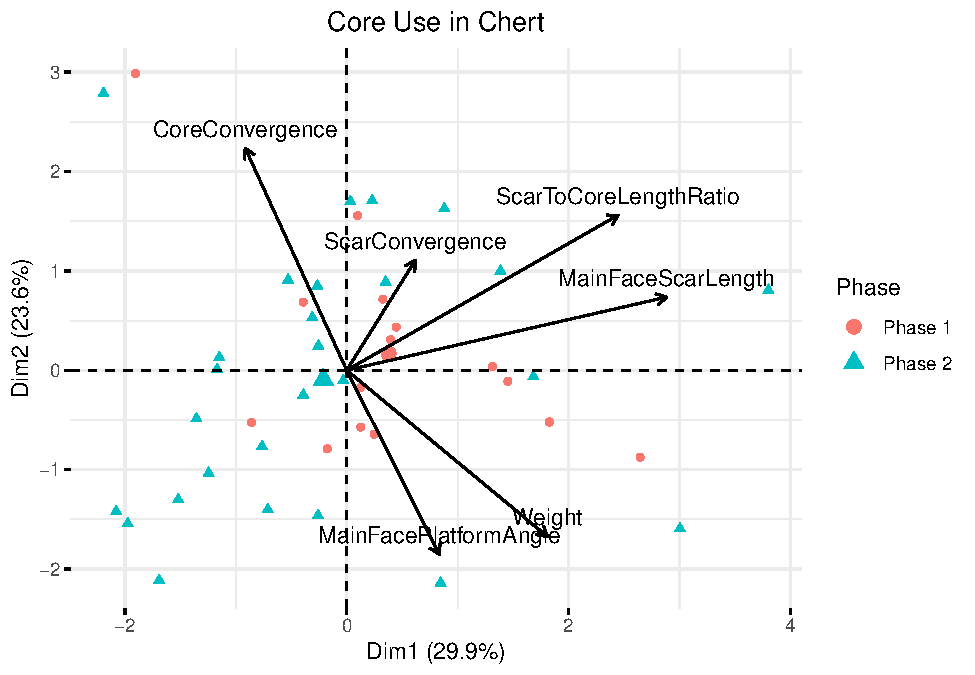
\includegraphics{thesis_files/figure-latex/unnamed-chunk-16-1.pdf}
\caption{\label{fig:unnamed-chunk-16}Variable plot of the first and second components of the Core Use PCA on chert (CUC).}
\end{figure}
\begin{table}[!h]

\caption{\label{tab:unnamed-chunk-17}Positive and negative principal component scores, Core Use PCA (CUC).}
\centering
\begin{tabular}[t]{lc>{\raggedright\arraybackslash}p{3cm}>{\raggedright\arraybackslash}p{3cm}>{\raggedright\arraybackslash}p{3cm}}
\toprule
\multicolumn{1}{c}{\textbf{Dimensions}} & \multicolumn{1}{c}{\textbf{\% variability}} & \multicolumn{1}{>{\centering\arraybackslash}p{3cm}}{\textbf{+}} & \multicolumn{1}{>{\centering\arraybackslash}p{3cm}}{\textbf{-}} & \multicolumn{1}{>{\centering\arraybackslash}p{3cm}}{\textbf{Interpretation}}\\
\midrule
1 & 29.9\% & Scar to core length ratio, Main scar length, Weight, Main face P angle, Scar convergence & Core convergence & Less convergent cores appear associated with convergent and longer scars. Bigger core mass reduction seems related to convergent-shaped cores.\\
2 & 23.6\% & Core convergence, Scar to core length ratio, Main face scar length, Scar convergence & Weight, Main face P angle & As the core becomes more convergent, and scar convergence and length ratios increase, weight and angle decrease. As core mass reduces, the core become more shaped and convergent.\\
Cumulative \% & 53.5\% &  &  & \\
\bottomrule
\end{tabular}
\end{table}
For quartz, the two dimensions in core use explain a cumulative 62\% of variability, with dimension 1 representing 40.6\% and dimension 2 representing 21.4\% (table X), and thus, considerably less.

Dimension 1 shows a positive correlation between all variables, although with different representations. Core convergence, scar to core length ratio, main face platform angles and scar length all show high values in the positive loadings of Dim 1, which means there is an association between convergent cores and longer blanks.These values, however, might be influenced the the high percentage of represention a few invididuals seem to have, located on the further negative loadings of Dim 1, which are less convergent, with smaller and shorter scars. Despite those values, most individuals for both phases seem to be equaly located on the positive loadings or fairly close.

As for dimension 2, it shows a negative correlation between core convergence and scar convergence with weight, meaning that as weight reduces, cores become more convergent accompanied by more convergent scars as well, although these become smaller. Once again, this might represent core mass reduction through the shapping of the core. Upper 5/4E is better represented on the negative loadings of this dimension, showing a bigger quantity of heavier and less convergent individuals than Lower 5.
\begin{figure}
\centering
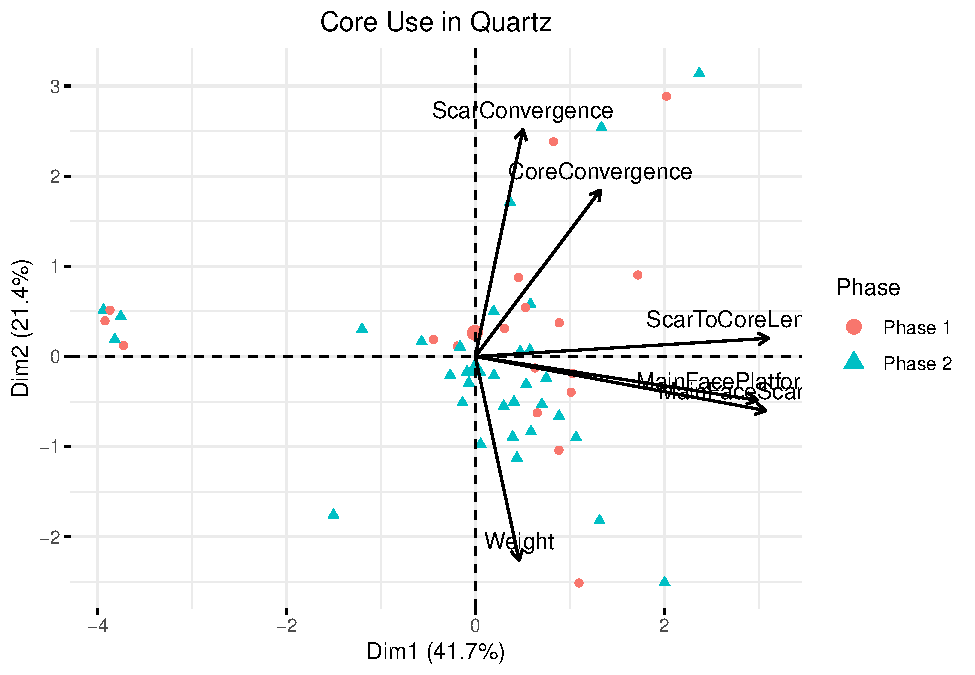
\includegraphics{thesis_files/figure-latex/unnamed-chunk-18-1.pdf}
\caption{\label{fig:unnamed-chunk-18}Variable plot of the first and second components of the Core Use PCA on quartz (CUQ).}
\end{figure}
\begin{table}[!h]

\caption{\label{tab:unnamed-chunk-19}Positive and negative principal component scores, Core Use PCA (CUQ).}
\centering
\begin{tabular}[t]{lc>{\raggedright\arraybackslash}p{3cm}>{\raggedright\arraybackslash}p{3cm}>{\raggedright\arraybackslash}p{3cm}}
\toprule
\multicolumn{1}{c}{\textbf{Dimensions}} & \multicolumn{1}{c}{\textbf{\% variability}} & \multicolumn{1}{>{\centering\arraybackslash}p{3cm}}{\textbf{+}} & \multicolumn{1}{>{\centering\arraybackslash}p{3cm}}{\textbf{-}} & \multicolumn{1}{>{\centering\arraybackslash}p{3cm}}{\textbf{Interpretation}}\\
\midrule
1 & 40.6\% & Scar to core length ratio, Main scar length, Main face P angle &  & Convergent cores appear associated with convergent and smaller scars.\\
2 & 21.4\% & Core convergence, Scar to core length ratio & Weight, Main face P angle, Main face scar length & As the core becomes more convergent, and scar length ratios increase, weight decreases. Might represent core mass reduction through core shapping.\\
Cumulative \% & 62\% &  &  & \\
\bottomrule
\end{tabular}
\end{table}
The platform maintenance (BP) domain aims to explore how knappers controlled platform dimensions or used platform faceting to control flake length (Scerri et al 2014). On chert, the two dimensions of platform maintenance (BPC) explain 43.2\% of the samples variability. The decrease on cumulative percentages comparatively to cores might be explained by either the internal higher variability of flakes or the increase sample size.

Dimension 1 explains 25.9\% of variance. Low elongation is correlated positively with high platform flattening, on the positive loadings, while high elongation is correlated with low flattening. This might indicate similar sized blanks might he controlled by how deep the knapper strikes into the platform (Scerri et al.~2014). This dimension also shows the association of other types of platform preparation, winged and dihedral platforms with low elongation values, while plain platforms seem mostly associated with high elongation, although showing less contribution than other variables.

Dimension 2, which explains 17.3\% of sample variance, show an association of medium elongation with crushed platforms, which may reflect atypical flakes, with unprepared production compared to either low elongation (which should represent flakes) and high elongation blanks. Comparatively, high and low elongation values show association with other types of platforms, which included faceted platforms.

For both dimensions, neither Lower 5 or 2 show particular differences, both showing equal internal variability regarding the variables chosen for the MCA.
\begin{figure}
\centering
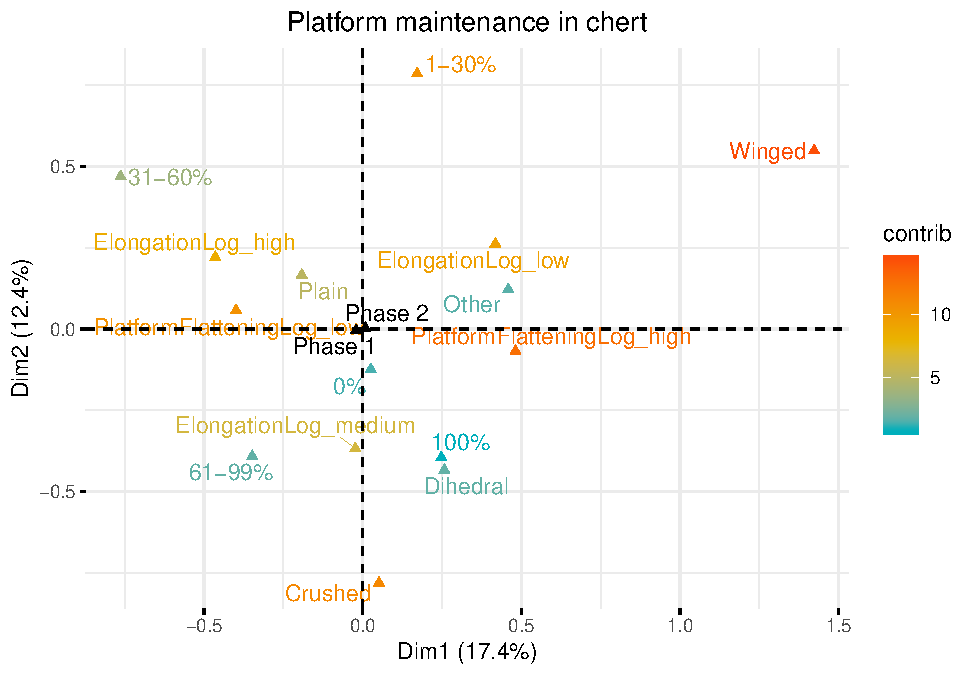
\includegraphics{thesis_files/figure-latex/unnamed-chunk-20-1.pdf}
\caption{\label{fig:unnamed-chunk-20}Variable plot of the first and second components of the blanks Platform Maintenance PCA on chert (BPC).}
\end{figure}
\begin{table}[!h]

\caption{\label{tab:unnamed-chunk-21}Positive and negative principal component scores, blank Platform Maintenance PCA (CUC).}
\centering
\begin{tabular}[t]{lc>{\raggedright\arraybackslash}p{3cm}>{\raggedright\arraybackslash}p{3cm}>{\raggedright\arraybackslash}p{3cm}}
\toprule
\multicolumn{1}{c}{\textbf{Dimensions}} & \multicolumn{1}{c}{\textbf{\% variability}} & \multicolumn{1}{>{\centering\arraybackslash}p{3cm}}{\textbf{+}} & \multicolumn{1}{>{\centering\arraybackslash}p{3cm}}{\textbf{-}} & \multicolumn{1}{>{\centering\arraybackslash}p{3cm}}{\textbf{Interpretation}}\\
\midrule
1 & 25.9\% & Low elongation, High P flattening, Winged platform, Dihedral platform, Other platform & High elongation, Low P flattening, Plain platform & Similar sizes of blanks might he controlled by how deep the knapper strikes into the platform.\\
2 & 17.3\% & High elongation, Low elongation, Other platform & Medium elongation, Crushed platform & High and low elongations seem to be controlled by specific types of platforms, while medium elongations are strongly correlated to crushed platforms.\\
Cumulative \% & 43.2\% &  &  & \\
\bottomrule
\end{tabular}
\end{table}
Regarding platform maintenance on quartz (BPQ), the two main dimensions explain 54.4\% of the sample.

Dimension 1, which explains 31\% of variability, shows the association between high elongation scores and low flattening, although for quartz, other types of platforms seem to correlate positively as well. Low elongation is correlated with high platform flattening values, however, and with plain platforms although, once again, this variable seems to contribute less than others. These patterns may represent differences in platform preparation and platform striking to control blank shape between raw materials.

Dimension 2, representing 23.4\% of variability, shows medium elongation values on the negative area, where high and low elongation are found on the positive axis, as well as other types of platform. This may reflect an intermediate blank with no particular preparation, while high elongation blanks are more often achieved with resource to specific platform types.

Alike on chert, Lower 5 and Upper 5/4E don't show significant differences between each other, both represented at the centre of the MCA.
\begin{figure}
\centering
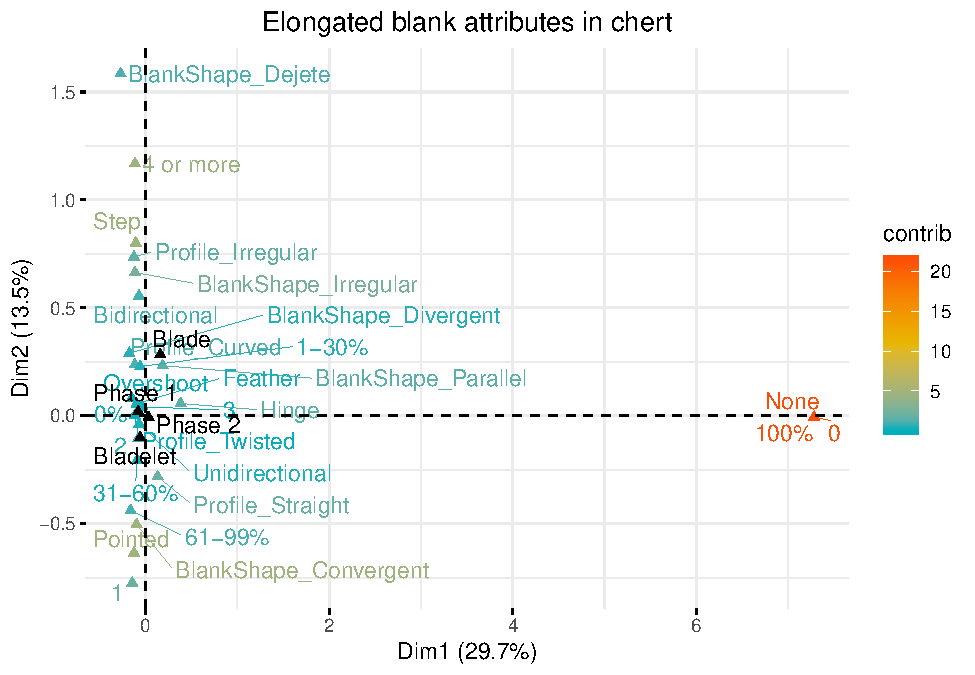
\includegraphics{thesis_files/figure-latex/unnamed-chunk-22-1.pdf}
\caption{\label{fig:unnamed-chunk-22}Variable plot of the first and second components of the blanks Platform Maintenance PCA on quartz (BPQ).}
\end{figure}
\begin{table}[!h]

\caption{\label{tab:unnamed-chunk-23}Positive and negative principal component scores, blank Platform Maintenance PCA (CUQ).}
\centering
\begin{tabular}[t]{lc>{\raggedright\arraybackslash}p{3cm}>{\raggedright\arraybackslash}p{3cm}>{\raggedright\arraybackslash}p{3cm}}
\toprule
\multicolumn{1}{c}{\textbf{Dimensions}} & \multicolumn{1}{c}{\textbf{\% variability}} & \multicolumn{1}{>{\centering\arraybackslash}p{3cm}}{\textbf{+}} & \multicolumn{1}{>{\centering\arraybackslash}p{3cm}}{\textbf{-}} & \multicolumn{1}{>{\centering\arraybackslash}p{3cm}}{\textbf{Interpretation}}\\
\midrule
1 & 31\% & High elongation, Low P flattening, Crushed platform, Other platform & Low elongation, High P flattening, Plain platform & Attempts to control length through platform flattening and platform type.\\
2 & 23.4\% & High elongation, Low elongation, High P flattening, Other platform, Crushed platform & Medium elongation, Low P flattening, Plain platform & High and low elongations seem to be controlled by specific types of platforms, while medium elongations are better correlated to low P flattening and plain platforms.\\
Cumulative \% & 54.4\% &  &  & \\
\bottomrule
\end{tabular}
\end{table}
Dorsal surface convexity (BD) on chert shows a cumulative percentage of 39.8\% for both principal dimensions, with dimension 1 representing 28.1\% of sample variance, and dimension 2 representing 11.7\%, much lower frequencies than the first.

Dimension 1 shows an association between high elongation, low vertical convexity, convergent and parallel shapes, triangular and trapezoidal cross sections and straight profiles. This may signify control of elongation through morphological characteristics or represent a reduction sequence for elongated blanks with preferential blank characteristics, as opposed to the negative loadings in this dimensions, which show low elongations correlated with irregular morphological attributes or other shapes.

Dimension 2, which as seen, explains much less variability, differentiates between two groups: a group with irregular attributes and a group with other attributes such as lenticular cross sections or ``other'' blank shapes, showing that there is a group of blanks, correlated with low elongation, which shows much more irregular characteristics than the other two identified blank groups.

There seems to exist a difference between phases, where Upper 5/4E is relatively centered, though pulling towards the negative dimension 1 axis, and thus towards the high elongation, convergent/parallel with triangular cross section blanks, and Lower 5 is further into the positive axis. This slight difference between phases might represent a difference in blank production between Lower 5 and Upper 5/4E, which might be understood as the result of the presence of Vale Comprido points in Upper 5/4E, which are represented by a specific type of elongated blanks with convergent shapes, absent from Lower 5.
\begin{figure}
\centering
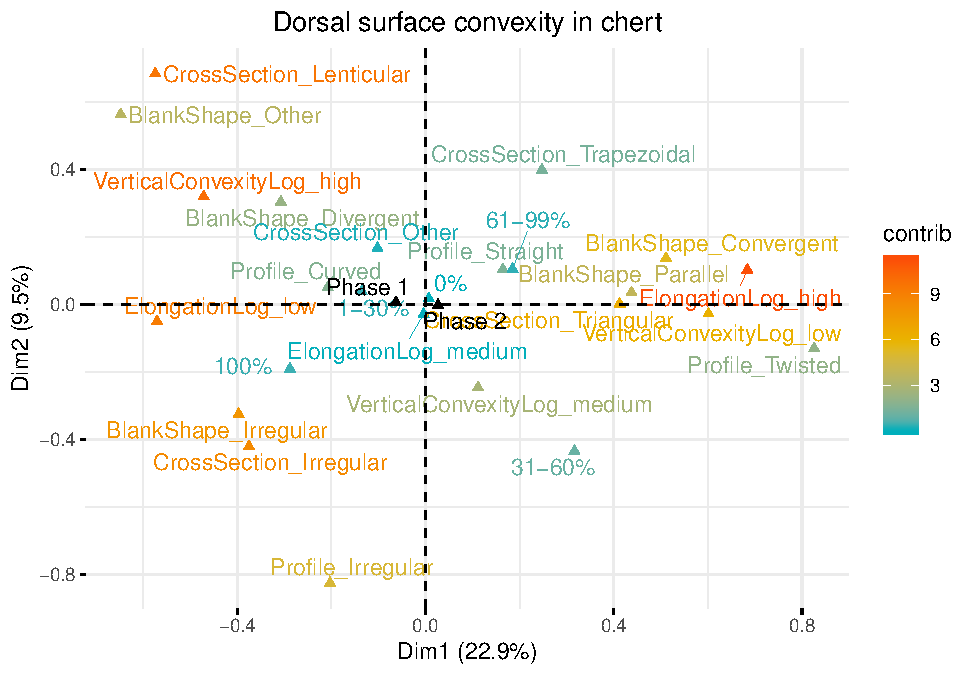
\includegraphics{thesis_files/figure-latex/unnamed-chunk-24-1.pdf}
\caption{\label{fig:unnamed-chunk-24}Variable plot of the first and second components of the blanks Dorsal Convexity PCA on chert (BDC).}
\end{figure}
\begin{table}[!h]

\caption{\label{tab:unnamed-chunk-25}Positive and negative principal component scores, blank Dorsal Convexity PCA (BDC).}
\centering
\begin{tabular}[t]{lc>{\raggedright\arraybackslash}p{3cm}>{\raggedright\arraybackslash}p{3cm}>{\raggedright\arraybackslash}p{3cm}}
\toprule
\multicolumn{1}{c}{\textbf{Dimensions}} & \multicolumn{1}{c}{\textbf{\% variability}} & \multicolumn{1}{>{\centering\arraybackslash}p{3cm}}{\textbf{+}} & \multicolumn{1}{>{\centering\arraybackslash}p{3cm}}{\textbf{-}} & \multicolumn{1}{>{\centering\arraybackslash}p{3cm}}{\textbf{Interpretation}}\\
\midrule
1 & 28.2\% & Low elongation, Lenticular cross section, High vertical convexity, Other blankshape,
                              Blank shape irregular, Cross section irregular, Profile irregular & High elongation, Low vertical convexity, Convergent blankshape, Parallel blankshape, Triangular cross section,
                               Straight profile, Trapezoidal cross section & Represents the production of elongated blanks with convergent or parallel shapes and triangular cross sections,
                               against other more variable groups of blanks with lower elongations.\\
2 & 11.7\% & Lenticular cross section, High vertical convexity, Other blankshape & Irregular blank shape, Irregular section, Irregular profile & Group of variable blanks with high vertical convexity and variable attributes against a group of irregular blanks.\\
Cumulative \% & 39.8\% &  &  & \\
\bottomrule
\end{tabular}
\end{table}
The two main dimensions in the dorsal surface convexity domain on quartz (BDQ) have explain 35.6\% of the assemblage's variability.
Dimension 1, which explains 23.6\%, shows the association of high elongation, parallel shapes, triangular cross sections and low vertical convexities, in opposition to low elongation, more irregular blanks or with other attributes such as ``other'' blank shapes, high vertical convexities and lenticular cross sections.

Dimension 2 explains only 12\% of variability, opposing, alike chert, a group of irregular blanks with the other group of ``other'' blank shapes, lenticular cross sections, high vertical convexities and low elongations.

Once again, the association of these particular groups may show three similar types of products, with high elongation products having the same preferential attributes, although, on quartz, the difference between phases isn't as obvious as with chert.
Accepting the combination of elongated blanks with convergent shapes a by-product of Vale Comprido operative sequences, the lack of relevance of that shape on this MCA and the lack of differentiation between phases might be result of the inexistence of these types of retouched products in quartz.
\begin{figure}
\centering
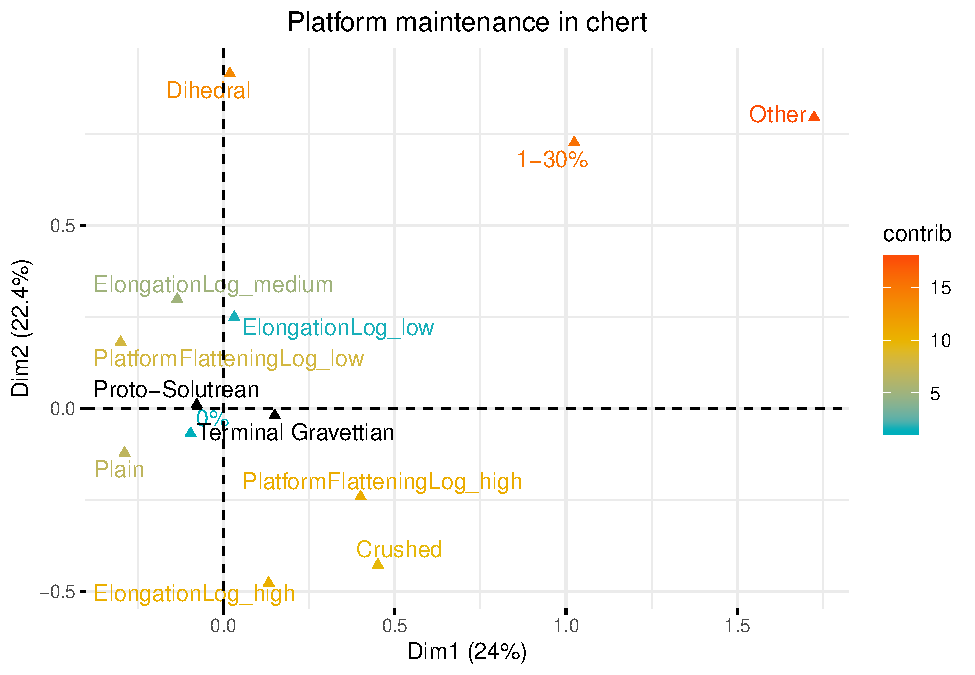
\includegraphics{thesis_files/figure-latex/unnamed-chunk-26-1.pdf}
\caption{\label{fig:unnamed-chunk-26}Variable plot of the first and second components of the blanks Dorsal Convexity PCA on quartz (BDQ).}
\end{figure}
\begin{table}[!h]

\caption{\label{tab:unnamed-chunk-27}Positive and negative principal component scores, blank Dorsal Convexity PCA (BDQ).}
\centering
\begin{tabular}[t]{lc>{\raggedright\arraybackslash}p{3cm}>{\raggedright\arraybackslash}p{3cm}>{\raggedright\arraybackslash}p{3cm}}
\toprule
\multicolumn{1}{c}{\textbf{Dimensions}} & \multicolumn{1}{c}{\textbf{\% variability}} & \multicolumn{1}{>{\centering\arraybackslash}p{3cm}}{\textbf{+}} & \multicolumn{1}{>{\centering\arraybackslash}p{3cm}}{\textbf{-}} & \multicolumn{1}{>{\centering\arraybackslash}p{3cm}}{\textbf{Interpretation}}\\
\midrule
1 & 23.6\% & Low elongation, Lenticular cross section, High vertical convexity, Other blankshape,
                              Blank shape irregular, Cross section irregular, Profile irregular & High elongation, Low vertical convexity, Parallel blankshape, Triangular cross section & Represents the production of elongated blanks with parallel shapes and triangular cross sections,
                               against other more variable groups of blanks with lower elongations.\\
2 & 12.1\% & Lenticular cross section, High vertical convexity, Other blankshape, Low elongation & Irregular blank shape, Irregular section, Irregular profile & Group of variable blanks with high vertical convexity and variable attributes against a group of irregular blanks.\\
Cumulative \% & 35.6\% &  &  & \\
\bottomrule
\end{tabular}
\end{table}
Core exploitation (CE) aims to understand the way knappers rotated cores, in order to create different dorsal surface convexity patterns (Scerri et al.~2014). The two main dimensions in chert (CEC) show a cumulative percentage of 51.5\%, explaining half of the sample's variability.

Dimension 1, which explains 37.8\% of variability, shows the correlation between more than 60\% cortex, no scars and other scar patterns (which most likely are mostly comprised by the variable ``none''). These represent early stages of blank removal, with cortical blanks or very high indexes of cortex, thus showing no scars and no patterns. In opposition to this group, there is on the negative axis of dim 1 other more variable reduction stages or strategies, generally characterized by low percentages of cortex.

Dimension 2, which explains much less variability (13.7\%), shows two different stages or strategies within the reduction sequence: correlation on the positive axis of dim 2 of bidirectional patterns on blanks with 3 to 4 or more dorsal scars, related with high elongation blanks; correlation on the negative axis of dim 2 between low elongation blanks, with 1 or 2 dorsal scars and unidirectional dorsal patterns. The understanding of dim 2 is however truncated since both groups lack obvious individualization, with only a couple variables standing out with stronger correlations, such as bidirectional patterns with 4 or more dorsal scars, and presence of 1 dorsal scar with low elongation blanks.

Once again, there are no obvious differences between the phases, for either dimension.
\begin{figure}
\centering
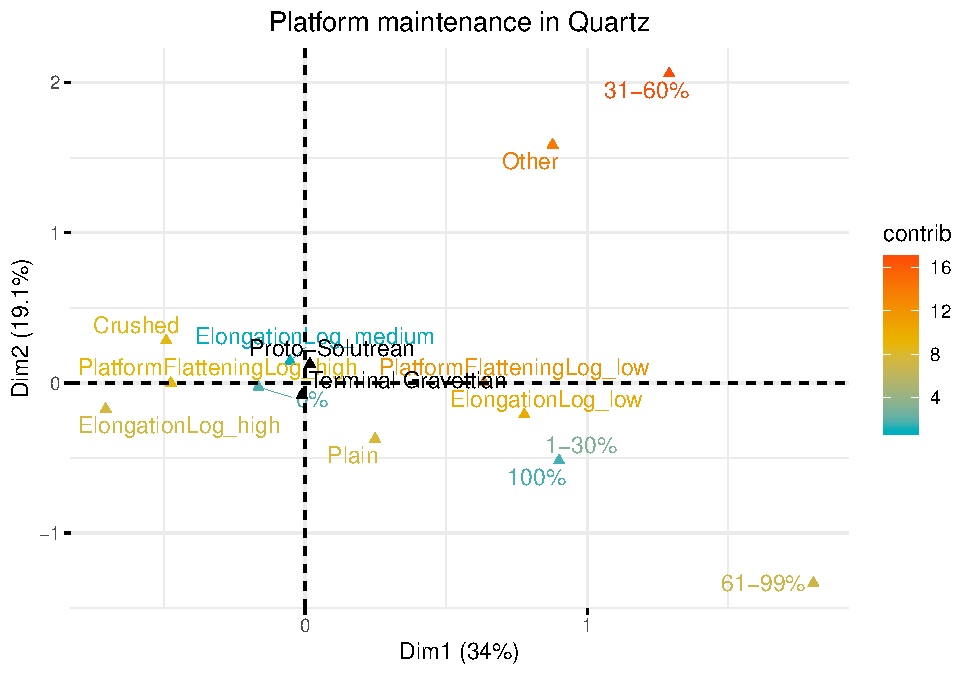
\includegraphics{thesis_files/figure-latex/unnamed-chunk-28-1.pdf}
\caption{\label{fig:unnamed-chunk-28}Variable plot of the first and second components of the blanks Core Exploitation PCA on chert (CEC).}
\end{figure}
\begin{table}[!h]

\caption{\label{tab:unnamed-chunk-29}Positive and negative principal component scores, blank Core Exploitation PCA (CEC).}
\centering
\begin{tabular}[t]{lc>{\raggedright\arraybackslash}p{3cm}>{\raggedright\arraybackslash}p{3cm}>{\raggedright\arraybackslash}p{3cm}}
\toprule
\multicolumn{1}{c}{\textbf{Dimensions}} & \multicolumn{1}{c}{\textbf{\% variability}} & \multicolumn{1}{>{\centering\arraybackslash}p{3cm}}{\textbf{+}} & \multicolumn{1}{>{\centering\arraybackslash}p{3cm}}{\textbf{-}} & \multicolumn{1}{>{\centering\arraybackslash}p{3cm}}{\textbf{Interpretation}}\\
\midrule
1 & 37.8\% & More than 60\% cortex, Other dorsal pattern, 0 scar count & 4 or more scar count, 3 scar count, 2 scar count, 0\% cortex, Unidirectional dorsal pattern, Bidirecional scar pattern & Associated with an earlier stage of production with more cortex against later stages of production\\
2 & 13.7\% & High elongation, 4 or more scar count, Bidirectional dorsal pattern & More then 60\% cortex, Unidirectional dorsal pattern, 2 scar count, Low elongation & Existance of a group of elongated products which show several negatives with bidirectional dorsal patterns 
                               against a group of less elongated, with 2 negatives and unidirectional dorsal patterns.\\
Cumulative \% & 51.5\% &  &  & \\
\bottomrule
\end{tabular}
\end{table}
On quartz (CEQ), the two main dimensions explain a cumulative percentage of 49.5\%, where dimensions 1 explains 33.6\%, and once again, dimension 2 explains a much smaller percentage (15.9\%).

Dimension 1 shows the association of more than 60\% cortex, ``other'' scar patterns (mostly comprised of variable ``none'') and ``other'' scar count (comprised mostly of ``0'' values), representing, alike chert, an early moment of core reduction, in opposition to the other more advanced reduction stages.

Dimension 2 seems to differentiate as well two groups of differing reduction strategies, alike chert. There is the correction between high elongation with dorsal scar counts of 2 and 3, on the negative axis, while on the positive there is the association between 31-60\% and 1-30\% cortex, dorsal scar counts of 1 and low elongations. This may represent an early stage of core reduction as well, where less elongated blanks still have cortex and have less scars, in comparison to a later stage of reduction, where the desired elongated products have more scars and much less cortex.

Regarding phases, both Lower 5 and Upper 5/4E seem very alike on quartz, almost completely overlapping at the centre of both dimensions axis.
\begin{figure}
\centering
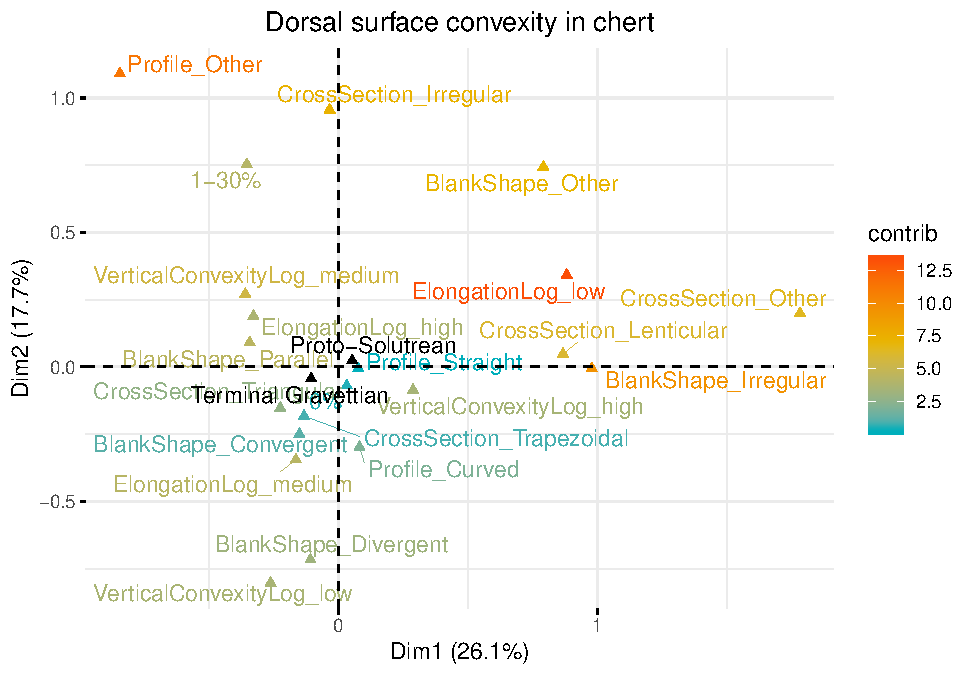
\includegraphics{thesis_files/figure-latex/unnamed-chunk-30-1.pdf}
\caption{\label{fig:unnamed-chunk-30}Variable plot of the first and second components of the blanks Core Exploitation PCA on quartz (CEQ).}
\end{figure}
\begin{table}[!h]

\caption{\label{tab:unnamed-chunk-31}Positive and negative principal component scores, blank Core Exploitation PCA (CEQ).}
\centering
\begin{tabular}[t]{lc>{\raggedright\arraybackslash}p{3cm}>{\raggedright\arraybackslash}p{3cm}>{\raggedright\arraybackslash}p{3cm}}
\toprule
\multicolumn{1}{c}{\textbf{Dimensions}} & \multicolumn{1}{c}{\textbf{\% variability}} & \multicolumn{1}{>{\centering\arraybackslash}p{3cm}}{\textbf{+}} & \multicolumn{1}{>{\centering\arraybackslash}p{3cm}}{\textbf{-}} & \multicolumn{1}{>{\centering\arraybackslash}p{3cm}}{\textbf{Interpretation}}\\
\midrule
1 & 33.6\% & More than 60\% cortex, Other dorsal pattern, Other scar count & 1-30\% cortex, 0\% cortex, High elongation, Unidirectional dorsal pattern, 1 scar count & Associated with an earlier stage of production with more cortex against later stages of production, with the
                               tendency for less presence of cortex, high elongation and unidirectional strategies.\\
2 & 16\% & 31-60\% cortex, 1-30\% cortex, Low elongation, 1 scar count & High elongation, Other dorsal pattern, Other scar count, 3 scar count, 2 scar count & Existance of a group of elongated products which show several negatives with variable dorsal patterns 
                               against a group of less elongated blanks.\\
Cumulative \% & 49.6\% &  &  & \\
\bottomrule
\end{tabular}
\end{table}
Since PCAs and MCAs on the domains shown on table X were applied to all blanks, which included the elongated blanks as well, instead of running them again on this particular sample, severely limiting the numbers and variability, instead some variables with impact on morphology were chosen, in order to understand morphological and technological patterns on elongated blanks. As such, the domain elongated blanks attributes (EA) was applied for chert (EAC) and quartz (EAQ) individually. For EA, two qualitative supplementary variables were considered: phase, as previous PCAs and MCAs; elongated blank type (bladelet and blade), in order to understand possible morphological preferences for each type, which might help understand whether there is the existence of two separate production strategies, or a continuous reduction of cores and thus blank size.

The two main dimensions of EAC explain 39\% of the sample variability, dimension 1 explaining 20.2\% and dimension 2 explaining 18.8\%.
Dimension 1 shows a strong association between an earlier moment of reduction, with no dorsal scar patterns and 0 scars, differing from the rest of the products which belong to a later stage of reduction. This may be interpreted as the existence of dedicated elongated blank production strategies, which start with already elongated entirely cortical products.

Dimension 2 shows the association between pointed terminations, convergent shapes, straight profiles, unidirectional patterns and 1 to 2 dorsal scars on the negative axis, and the correlation between curved profiles, parallel shapes, 4 or more dorsal scars, steps and degète terminations and bidirectional patterns.

Regarding the supplementary loadings, there seems to be some similarity between Lower 5 and 2, although the biggest differences occur within the elongated blank type. While bladelets fall further into the negative axis of dim 2, closer to the unidirectional, convergent and pointed blanks, blades fall onto the positive axis of dim 2, showing more correlation to curved profiles and more variability in terms of attributes and dorsal scar counts, which may indicate that smaller products have more standardized attributes than larger elongated blanks.
\begin{figure}
\centering
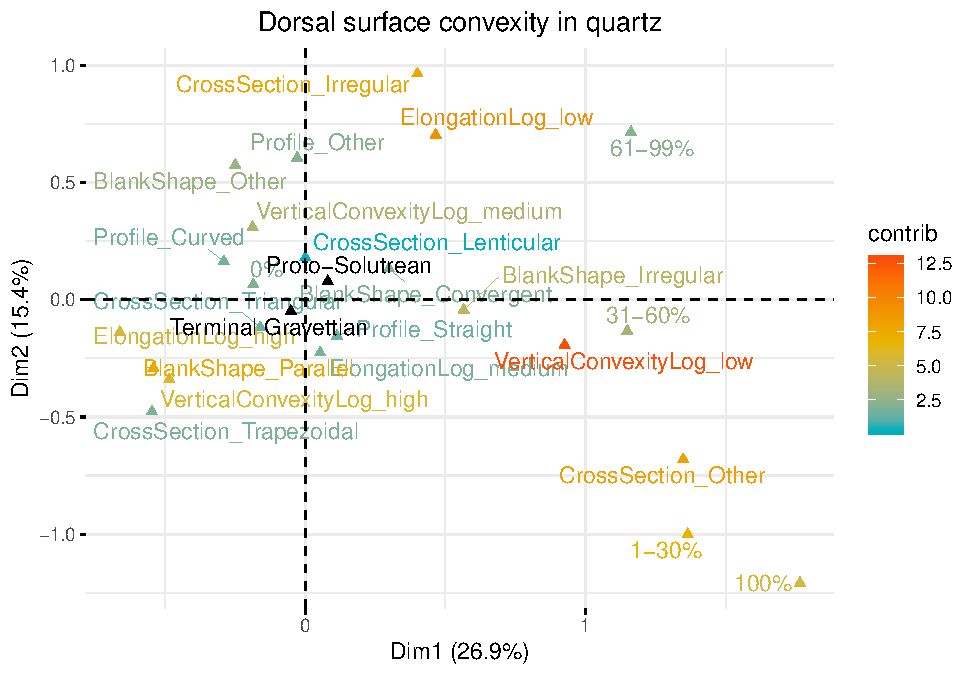
\includegraphics{thesis_files/figure-latex/unnamed-chunk-32-1.pdf}
\caption{\label{fig:unnamed-chunk-32}Variable plot of the first and second components of the Elongated product attributes PCA on chert (EAC).}
\end{figure}
\begin{table}[!h]

\caption{\label{tab:unnamed-chunk-33}Positive and negative principal component scores, Elongated product attributes PCA (EAC).}
\centering
\begin{tabular}[t]{lc>{\raggedright\arraybackslash}p{3cm}>{\raggedright\arraybackslash}p{3cm}>{\raggedright\arraybackslash}p{3cm}}
\toprule
\multicolumn{1}{c}{\textbf{Dimensions}} & \multicolumn{1}{c}{\textbf{\% variability}} & \multicolumn{1}{>{\centering\arraybackslash}p{3cm}}{\textbf{+}} & \multicolumn{1}{>{\centering\arraybackslash}p{3cm}}{\textbf{-}} & \multicolumn{1}{>{\centering\arraybackslash}p{3cm}}{\textbf{Interpretation}}\\
\midrule
1 & 20.2\% & 0 scar count, No dorsal pattern & 4 or more scar count, Degete blank shape, Divergent blank shape, Step termination & Existence of an earlier stage of production against a more variable set of elongated products.\\
2 & 18.8\% & 4 or more scar count, Degete blank shape, step termination, Bidirectional patterns & Pointed termination, Convergent blank shape, Straight profile, 2 scar count, Twisted termination,
                               Feather termination, Unidirectional dorsal pattern & Existence of two groups: pointed terminations, convergent shapes, straight profiles, unidirectional aptterns; curved profiles, parallel shapes, 4 or more dorsal scars and bidirectional patterns\\
Cumulative \% & 39\% &  &  & \\
\bottomrule
\end{tabular}
\end{table}
For quartz, the two main dimensions of EAQ explain 39.7\% of the sample's variability.

Dimension 1, which explains 23\%, shows a strong association between bidirectional scar patterns and 4 or more dorsal scar counts, a strong correlation which has already been established on previous MCAs. Once again, the other group seems to show the correlation between the rest of the attributes. What these associations show, however, is also the inexistence of a strongly correlated early stage of reduction specifically for elongated blanks in quartz.

Dimension 2, representing 16.7\% of variability, shows the association between curved profiles, convergent shapes, pointed terminations with 3 dorsal scars on the positive axis, while the negative axis, although contributing less, shows the association between parallel shapes, 1 to 2 dorsal scars, straight profiles, feathered terminations, both axis seemingly sharing the unidirectionality of dorsal scar patterns.

Unlike chert, there is no great difference between Lower 5 and 2, neither between bladelets and blades, hinting to perhaps a continuous production strategy for both large and small elongated blanks, instead of two different sequences for the obtention of blades and bladelets.
\begin{figure}
\centering
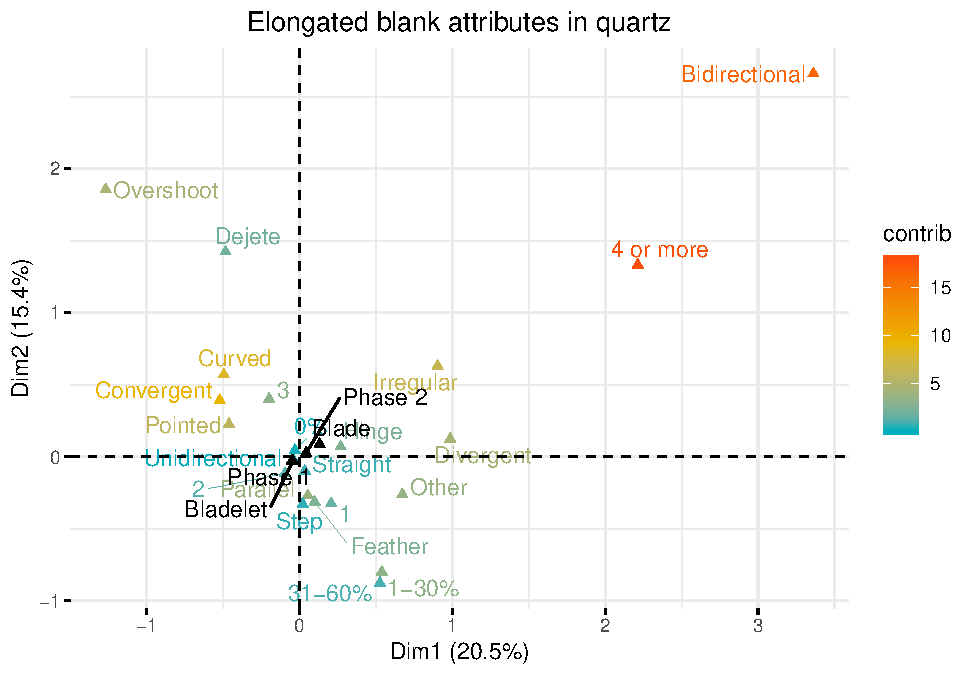
\includegraphics{thesis_files/figure-latex/unnamed-chunk-34-1.pdf}
\caption{\label{fig:unnamed-chunk-34}Variable plot of the first and second components of the Elongated product attributes PCA on quartz (EAQ).}
\end{figure}
\begin{table}[!h]

\caption{\label{tab:unnamed-chunk-35}Positive and negative principal component scores, Elongated product attributes PCA (EAQ).}
\centering
\begin{tabular}[t]{lc>{\raggedright\arraybackslash}p{3cm}>{\raggedright\arraybackslash}p{3cm}>{\raggedright\arraybackslash}p{3cm}}
\toprule
\multicolumn{1}{c}{\textbf{Dimensions}} & \multicolumn{1}{c}{\textbf{\% variability}} & \multicolumn{1}{>{\centering\arraybackslash}p{3cm}}{\textbf{+}} & \multicolumn{1}{>{\centering\arraybackslash}p{3cm}}{\textbf{-}} & \multicolumn{1}{>{\centering\arraybackslash}p{3cm}}{\textbf{Interpretation}}\\
\midrule
1 & 23\% & Bidirectional dorsal pattern, 4 or more scar count & 3 scar count, Curved profile, Convergent shape, Pointed termination, Overshoot termination & Existence of a group of elongated blanks with bidirecional pattern and several scars
                               without the presence of an early stage of reduction.\\
2 & 16.7\% & Bidirectional dorsal pattern, 4 or more scar count, Convergent shape, Pointed termination, Overshoot termination,
                               Degete termination, 3 scar count & 1 scar count, 2 scar count, Parallel shape, Feather termination, Straight profile & Group of preferential association between curved profiles, convergent shapes and pointed terminations, and parallel shapes, straight profiles and feathered terminations, all with unidirectional patterns.\\
Cumulative \% & 39.7\% &  &  & \\
\bottomrule
\end{tabular}
\end{table}
\hypertarget{lapa-do-picareiro-8}{%
\subsubsection{Lapa do Picareiro}\label{lapa-do-picareiro-8}}

Following the methodologies already described, the blank attributes were divided into domains (table x), separated by chert and quartz, the most present raw materials, which were analysis by MCAs. Cores were not, however, due to the low sample, and thus, low existing variability.

Blank platform maintenance (BP) shows two dimensions which explain 52\% of the total assemblage's variability.

Dimension 1, which explains 27.5\%, shows a correlation between high elongation with high platform flattening values, crushed and other types of platforms. On the negative axis, low platform flattening values are associated with dihedral platforms and medium elongation, which might indicate that blanks might have been controlled by platform depth and preparation, although plain platforms are recurring in all elongation ratios.

Dimension 2, explaining 24.5\% of variability, shows on the negative axis, high elongation values associated with low flattening, plain and crushed platforms, while the positive axis is represented by low elongation with high platform flattening values, dihedral and other platforms, which once again seems to show blank elongation through platform depth, perhaps more than platform type.

The supplementary variables show some differences, where the U/Lower T group seems further pulled into the high elongation and high flattening log, which might represent a knapping strategy most present in this group, while the Middle T is closer to the centre, and thus seemingly much more variable.
\begin{figure}
\centering
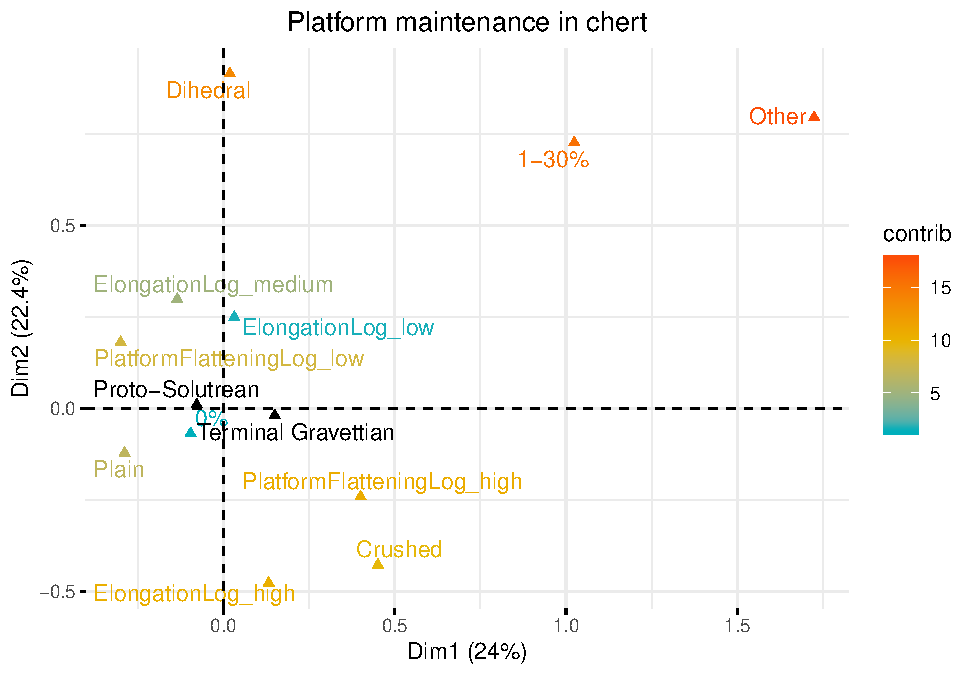
\includegraphics{thesis_files/figure-latex/unnamed-chunk-36-1.pdf}
\caption{\label{fig:unnamed-chunk-36}Variable plot of the first and second components of the blanks Platform Maintenance PCA on chert (BPC).}
\end{figure}
\begin{table}

\caption{\label{tab:unnamed-chunk-37}Positive and negative principal component scores, blank Platform Maintenance PCA (CUC).}
\centering
\begin{tabular}[t]{lc>{\raggedright\arraybackslash}p{3cm}>{\raggedright\arraybackslash}p{3cm}>{\raggedright\arraybackslash}p{3cm}}
\toprule
\multicolumn{1}{c}{\textbf{Dimensions}} & \multicolumn{1}{c}{\textbf{\% variability}} & \multicolumn{1}{>{\centering\arraybackslash}p{3cm}}{\textbf{+}} & \multicolumn{1}{>{\centering\arraybackslash}p{3cm}}{\textbf{-}} & \multicolumn{1}{>{\centering\arraybackslash}p{3cm}}{\textbf{Interpretation}}\\
\midrule
1 & 27.5\% & High elongation, High flattening, Other platform, Crushed platform & Low platform flattening, Dihedral platform, Medium elongation & Similar sizes of blanks might he controlled by how deep the knapper strikes into the platform or by platform morphology.\\
2 & 24.5\% & Other platform, High flattening, Low elongation, Dihedral platform & High elongation, Low P flattening, Plain platform, Crushed platform & Similar sizes of blanks might he controlled by how deep the knapper strikes into the platform.\\
Cumulative \% & 52\% &  &  & \\
\bottomrule
\end{tabular}
\end{table}
Regarding platform maintenance in quartz, the two main dimensions explain 71.2\% of the sample's variability, Dim 1 explaining 48.2\% and Dim 2 explaining considerably less (23\%). These high values might be related to either assemblage size, since the samples for Lapa do Picareiro are much smaller than those for Vale Boi, or simply by internal assemblage variability, since Lapa do Picareiro doesn't seem to have the presence in situ of a complete reduction sequence.

Dimension 1, on the positive axis, has the association between low elongation and low platform flattening values, associated with plain platforms and other platforms. On the negative axis there is high elongation values with high flattening and crushed platforms, which, once again, might represent the control of blank elongation by how deep into the platform the knapper hits.

Dimension 2 shows on the negative axis the correlation between high and low elongations and plain platforms, while on the positive axis there are medium elongations and other platforms, crushed platforms and low platform flattening values. This axis might represent probable differences between high and low elongations mostly represented by plain platforms, from intermediate elongation products.

Similarly to chert, the supplementary variables seem to show some differences between the two groups, where the Middle T seems closer to the medium elongation products while the Terminal Gravettin gravitates close to the centre of both dimensions.
\begin{figure}
\centering
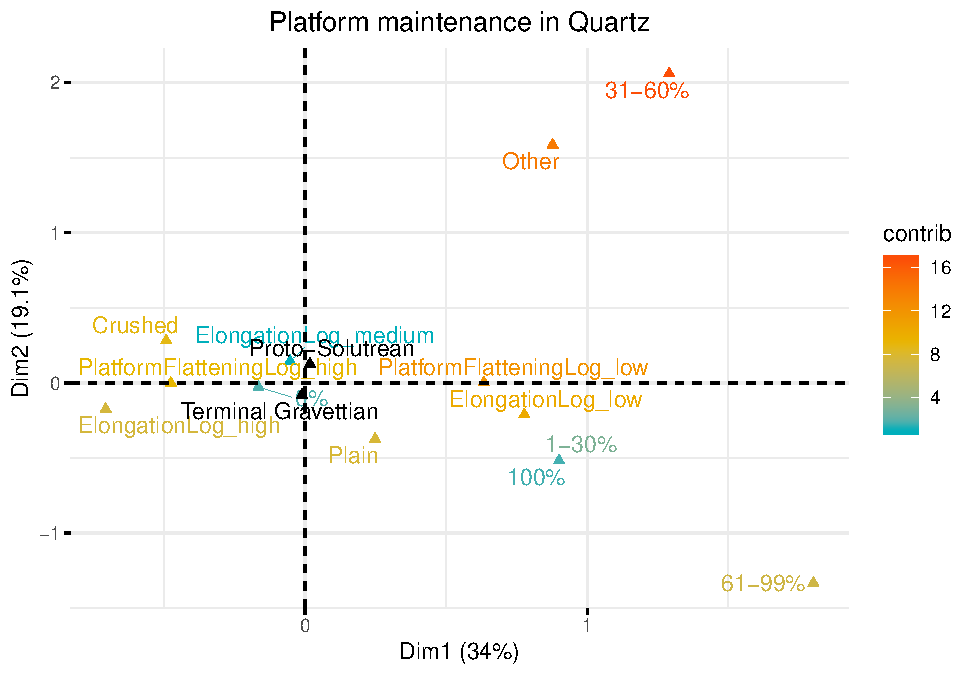
\includegraphics{thesis_files/figure-latex/unnamed-chunk-38-1.pdf}
\caption{\label{fig:unnamed-chunk-38}Variable plot of the first and second components of the blanks Platform Maintenance PCA on quartz (BPQ).}
\end{figure}
\begin{table}

\caption{\label{tab:unnamed-chunk-39}Positive and negative principal component scores, blank Platform Maintenance PCA (CUC).}
\centering
\begin{tabular}[t]{lc>{\raggedright\arraybackslash}p{3cm}>{\raggedright\arraybackslash}p{3cm}>{\raggedright\arraybackslash}p{3cm}}
\toprule
\multicolumn{1}{c}{\textbf{Dimensions}} & \multicolumn{1}{c}{\textbf{\% variability}} & \multicolumn{1}{>{\centering\arraybackslash}p{3cm}}{\textbf{+}} & \multicolumn{1}{>{\centering\arraybackslash}p{3cm}}{\textbf{-}} & \multicolumn{1}{>{\centering\arraybackslash}p{3cm}}{\textbf{Interpretation}}\\
\midrule
1 & 48.2\% & Low P flattening, Low elongation, Plain platform, Other platform & High elongation, High P flattening, Crushed platform & Similar sizes of blanks might he controlled by how deep the knapper strikes into the platform.\\
2 & 23\% & Medium elongation, Low P flattening, Crushed platform, Other platform & High elongation, Low elongation, Plain platform & Similar sizes of blanks might he controlled by how deep the knapper strikes into the platform, diffetianting between low and high elongation blanks from medium elongation blanks.\\
Cumulative \% & 71.2\% &  &  & \\
\bottomrule
\end{tabular}
\end{table}
The two dimensions of dorsal surface convexity in chert (BDC) show a cumulative percentage of 45.2\%, explaining almost half of the sample's variability.

Dimension 1, which explains 27.7\%, shows the correlation on the positive axis between low elongation and high vertical convexity with attributes which are represented less than 0.05\%, such is the case for other blank shapes, other cross sections, but also irregular blank shapes. On the negative axis, there is the correlation between high elongation, medium and low vertical convexity values, as well as several attributes such as parallel and convergent blank shapes, triangular and trapezoidal cross sections, and other types of profile. This might represent a higher frequency of standardization for elongated blanks, with parallel shapes and triangular/trapezoidal cross sections.

Dimension 2, explaining 17.5\% of variability, shows once again low and high elongations opposed to medium elongations, the latter associated with divergent blank shapes, low vertical convexity values, curved profiles and convergent blank shapes. This might represent different strategies to control elongation based on the morphology of dorsal convexity, although this domain seems better explained by dimension 1.

Once again, there seems to be a difference between the U/Lower T and Middle T groups, which appear in opposing axis. While U/Lower T shows more proximity towards the high elongation, parallel and triangular cross section correlations, the Middle T group seems closer to the low elongation group, a pattern already established in the previous domain.
\begin{figure}
\centering
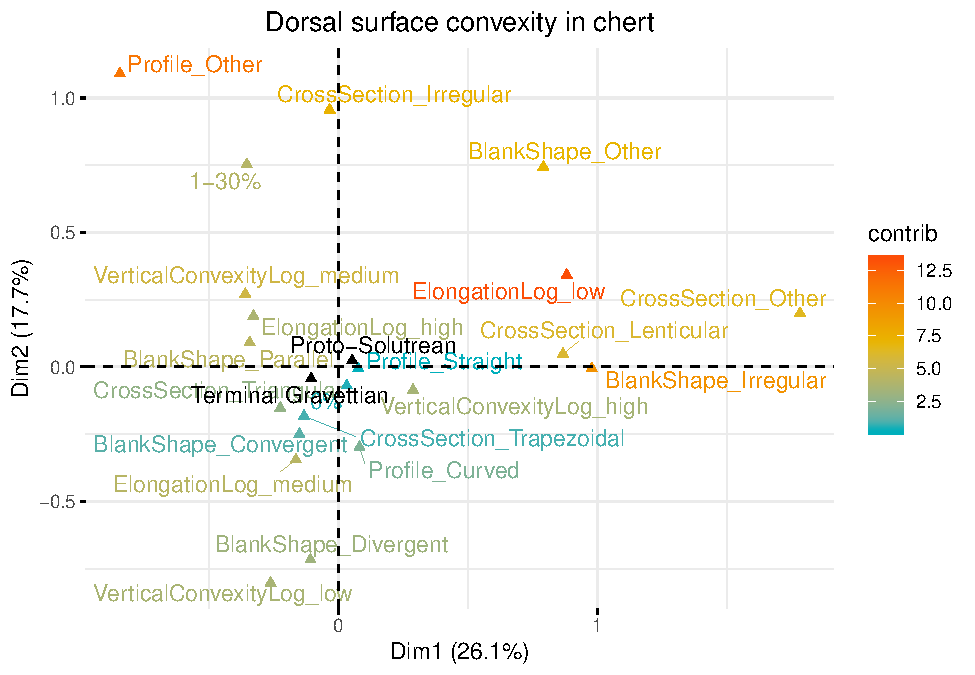
\includegraphics{thesis_files/figure-latex/unnamed-chunk-40-1.pdf}
\caption{\label{fig:unnamed-chunk-40}Variable plot of the first and second components of the blanks Dorsal Convexity PCA on chert (BDC).}
\end{figure}
\begin{table}

\caption{\label{tab:unnamed-chunk-41}Positive and negative principal component scores, blank Dorsal Convexity PCA (BDC).}
\centering
\begin{tabular}[t]{lc>{\raggedright\arraybackslash}p{3cm}>{\raggedright\arraybackslash}p{3cm}>{\raggedright\arraybackslash}p{3cm}}
\toprule
\multicolumn{1}{c}{\textbf{Dimensions}} & \multicolumn{1}{c}{\textbf{\% variability}} & \multicolumn{1}{>{\centering\arraybackslash}p{3cm}}{\textbf{+}} & \multicolumn{1}{>{\centering\arraybackslash}p{3cm}}{\textbf{-}} & \multicolumn{1}{>{\centering\arraybackslash}p{3cm}}{\textbf{Interpretation}}\\
\midrule
1 & 27.7\% & Low elongation, High vertical convexity, Other blankshape, Other cross section, Irregular blankshape, Lenticular cross section & High elongation, Medium vertical convexity, Low vertical convexity, Parallel blankshape, Convergent blankshape, Triangular cross section, Trapezoidal cross section, Other profile & Higher frequency of standardization for elongated blanks, through the control of their dorsal surface morphology.\\
2 & 17.5\% & High elongation, Low elongation, Other blankshape, Irregular cross section, Other profile, Other cross section & Blank shape divergent, Low vertical convexity, Medium elongation, Blank shape convergent, Curved profile, Convergent blankshape & Different strategies to control elongation based on the morphology of dorsal surface convexity.\\
Cumulative \% & 45.2\% &  &  & \\
\bottomrule
\end{tabular}
\end{table}
Regarding the dorsal convexity in quartz, the two main dimensions explain a cumulative percentage of 45\%, where Dim 1 explains 28.6\% and Dim 2 explains a much small percentage (16.4\%).

Dimension 1 shows the association between irregular blank attributes, low vertical convexities and other cross sections, low elongations and convergent blank shapes, on the positive axis, and high elongation with parallel shapes, high vertical convexities, trapezoidal, triangular and lenticular cross sections and curved profiles on the negative. This dimension may represent the existence of a higher standardization of more elongated blanks, where lower elongation blanks often show more irregular or varying attributes.

Dimension 2 shows the correlation between medium elongation blanks with low convexities, trapezoidal cross sections, straight profiles, and a wider variability of attributes on the negative axis, while high and low elongations are still on the opposed axis like on chert, although this dimensions explain much less the dimension 1.

Supplementary variables also seem to follow the patterns shown on chert, where the Middle T group shows a tendency closer to the less elongated blanks, while the U/Lower T group shows a slight tendency for more elongated blanks, the two groups again showing some differences in terms of technology.
\begin{figure}
\centering
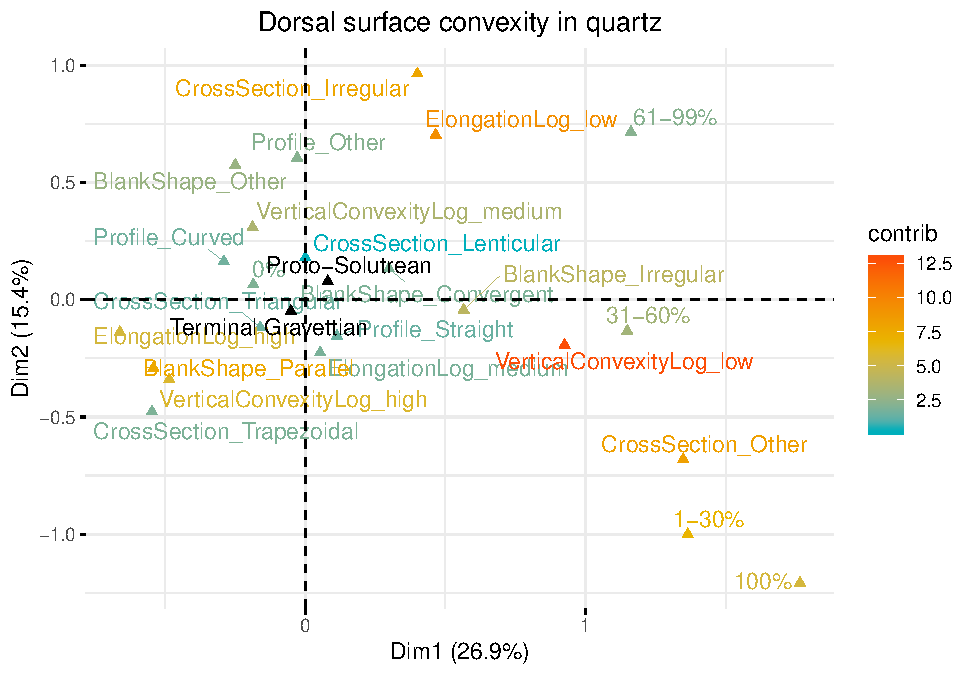
\includegraphics{thesis_files/figure-latex/unnamed-chunk-42-1.pdf}
\caption{\label{fig:unnamed-chunk-42}Variable plot of the first and second components of the blanks Dorsal Convexity PCA on quartz (BDQ).}
\end{figure}
\begin{table}

\caption{\label{tab:unnamed-chunk-43}Positive and negative principal component scores, blank Dorsal Convexity PCA (BDQ).}
\centering
\begin{tabular}[t]{lc>{\raggedright\arraybackslash}p{3cm}>{\raggedright\arraybackslash}p{3cm}>{\raggedright\arraybackslash}p{3cm}}
\toprule
\multicolumn{1}{c}{\textbf{Dimensions}} & \multicolumn{1}{c}{\textbf{\% variability}} & \multicolumn{1}{>{\centering\arraybackslash}p{3cm}}{\textbf{+}} & \multicolumn{1}{>{\centering\arraybackslash}p{3cm}}{\textbf{-}} & \multicolumn{1}{>{\centering\arraybackslash}p{3cm}}{\textbf{Interpretation}}\\
\midrule
1 & 28.6\% & Low elongation, Irregular cross section, Low vertical convexity, Irregular blank shape, Other cross section, Convergent blank shape & High elongation, Parallel blank shape, High vertical convexity, Trapezoidal cross section, Triangular cross section, Curved profile, Lenticular cross section & Existence of a higher standardization of more elongated blanks. Lower elongation blanks show more irregular or varying attributes.\\
2 & 16.4\% & Medium vertical convexity, Convergent blank shape, Other blankshape, Curved profile, High elongation, Low elongation, Irregular cross section & Low vertical convexity, Other cross section, Irregular blankshape, Trapezoidal cross sections, Straight profile, High vertical convexity, Medium elongation) & Differenciation in dorsal surface convexities and morphologies by blank elongation.\\
Cumulative \% & 45\% &  &  & \\
\bottomrule
\end{tabular}
\end{table}
Core exploitation on chert (CEC) explains, with its two main dimensions, 52.8\% of the sample's variability.

Dimension 1, which explains 30.6\%, shows the association between low elongation and 1 scar count, on the positive axis, and high and medium elongations related to 3 to 4 or more scars and low percentages of cortex presence. These associations seem to show the lack of an initial stage of reduction strategies, showing only the following less cortical stages.

Dimension 2, explaining 22.2\% of variability, shows a correlation between 2 scars with high elongation and unidirectional dorsal patterns on the negative axis, and 3 to 4 or more scars with use of other types of dorsal patterns. This shows the use of simple unidirectional strategies with less dorsal patterns, and other patterns with more dorsal patterns, which might reflect either different strategies or moments in the reduction sequence.

Differences between the U/Lower T and Middle T groups are more obvious in the dimension 1, once again reflecting differences in the elongations, with Middle T having lower elongation values comparatively to U/Lower T groups, although differences in dimension 2 are barely inexistent.
\begin{figure}
\centering
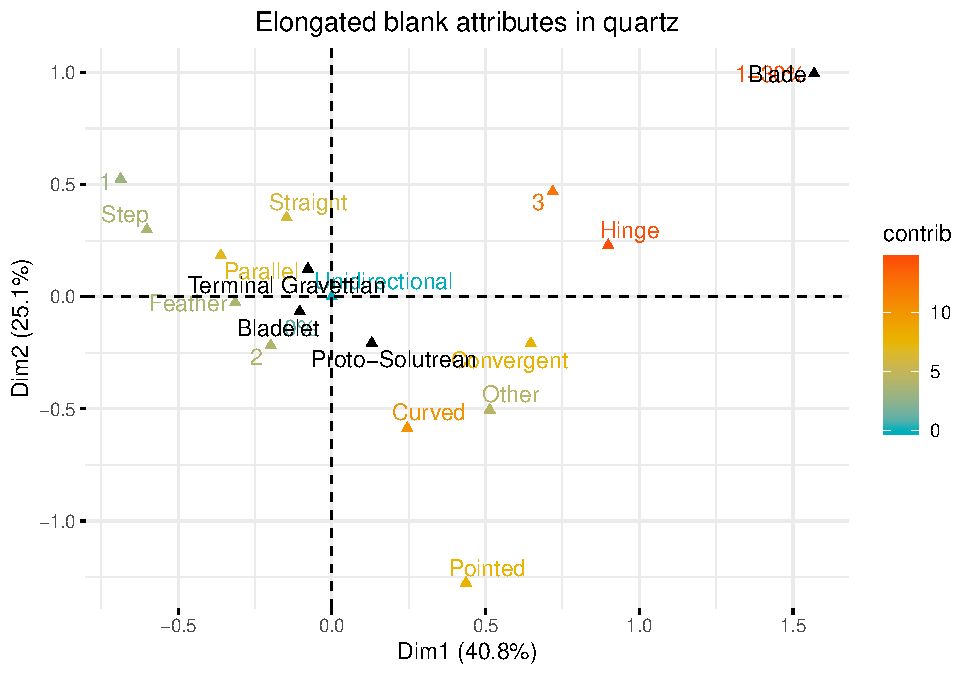
\includegraphics{thesis_files/figure-latex/unnamed-chunk-44-1.pdf}
\caption{\label{fig:unnamed-chunk-44}Variable plot of the first and second components of the blanks Core Exploitation PCA on chert (CEC).}
\end{figure}
\begin{table}

\caption{\label{tab:unnamed-chunk-45}Positive and negative principal component scores, blank Dorsal Convexity PCA (BDQ).}
\centering
\begin{tabular}[t]{lc>{\raggedright\arraybackslash}p{3cm}>{\raggedright\arraybackslash}p{3cm}>{\raggedright\arraybackslash}p{3cm}}
\toprule
\multicolumn{1}{c}{\textbf{Dimensions}} & \multicolumn{1}{c}{\textbf{\% variability}} & \multicolumn{1}{>{\centering\arraybackslash}p{3cm}}{\textbf{+}} & \multicolumn{1}{>{\centering\arraybackslash}p{3cm}}{\textbf{-}} & \multicolumn{1}{>{\centering\arraybackslash}p{3cm}}{\textbf{Interpretation}}\\
\midrule
1 & 30.6\% & Low elongation, 1 scar count & 1-30\% cortex, 3 scar count, 4 or more scar count, Medium elongation, High elongation & Existence of different stages of core reduction, without an initial cortical phase.\\
2 & 22.2\% & Other scar pattern, 1-30\% cortex, 3 scar count, 4 or more scar count & Unidirectional scar pattern, high elongation, 2 scar count & Use of simple unidirectional strategies with less dorsal patterns, and other patterns with more dorsal patterns. Possible diferent ways of core use at different stages of reduction.\\
Cumulative \% & 52.8\% &  &  & \\
\bottomrule
\end{tabular}
\end{table}
The two dimensions in core exploitation in quartz (CEQ) explain 56.9\% of the assemblage's variability, with dimension 1 representing 34.4\% and dimension 2 explaining 22.5\%.

Dimension 1 shows the association between low elongation, cortex percentages higher than 30\%, 1 scar count, other scar pattern and other scar count, on the positive axis, while on the negative axis are concentrated other more variable attributes, related to high elongations. This dimension might represent moments of early reduction (although without fully cortical pieces) and moments further into the reduction sequence, and with more scars and other patterns, in opposition to a more standardized group with less scars.

Dimension 2 shows exactly the difference between the already referred groups: one with 1 scar count and more than 60\% cortex, and another with other scar patterns and scar counts, possibly representing the difference between an initial stage of reduction (though not entirely cortical) and a more advanced and complex stage with a higher scar count. These three obviously separated groups might reflect the truncated reduction sequence present at Lapa do Picareiro.

The same pattern of supplementary variables as seen previously seems to repeat itself on the CEQ domain.
\begin{figure}
\centering
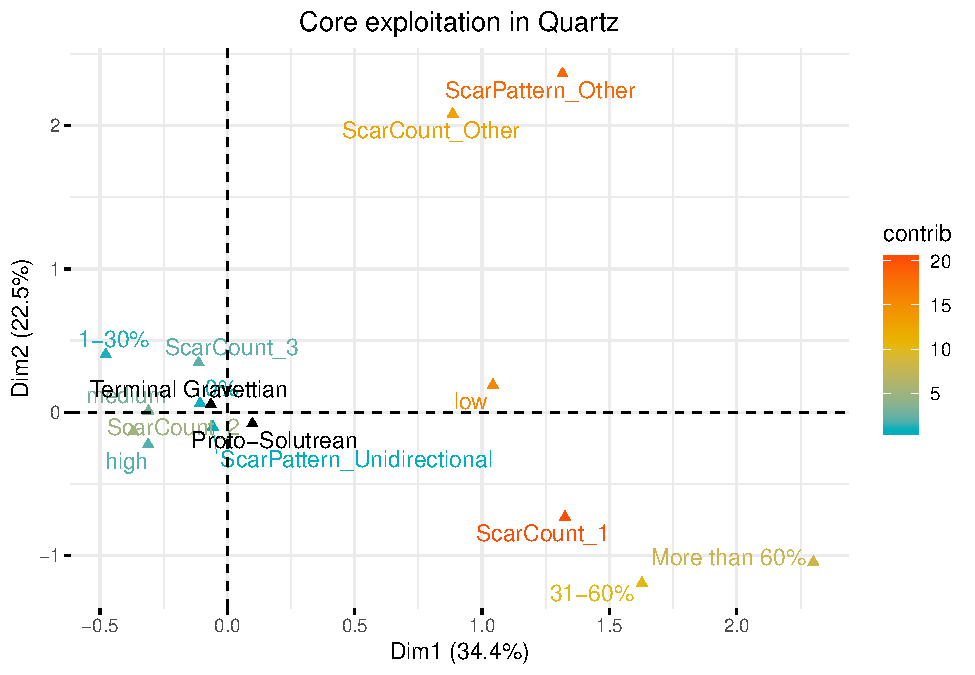
\includegraphics{thesis_files/figure-latex/unnamed-chunk-46-1.pdf}
\caption{\label{fig:unnamed-chunk-46}Variable plot of the first and second components of the blanks Core Exploitation PCA on quartz (CEQ).}
\end{figure}
\begin{table}

\caption{\label{tab:unnamed-chunk-47}Positive and negative principal component scores, blank Dorsal Convexity PCA (BDQ).}
\centering
\begin{tabular}[t]{lc>{\raggedright\arraybackslash}p{3cm}>{\raggedright\arraybackslash}p{3cm}>{\raggedright\arraybackslash}p{3cm}}
\toprule
\multicolumn{1}{c}{\textbf{Dimensions}} & \multicolumn{1}{c}{\textbf{\% variability}} & \multicolumn{1}{>{\centering\arraybackslash}p{3cm}}{\textbf{+}} & \multicolumn{1}{>{\centering\arraybackslash}p{3cm}}{\textbf{-}} & \multicolumn{1}{>{\centering\arraybackslash}p{3cm}}{\textbf{Interpretation}}\\
\midrule
1 & 34.4\% & Low elongation, 1 scar count, More than 60\% cortex, 31-60\% cortex, Other scar pattern, Other scar count & 1-30\% cortex, Medium elongation, High elongation, 3 scar count, 2 scar count & Existence of different stages of core reduction, without an initial completely cortical phase.\\
2 & 22.5\% & Other scar pattern, Other scar count & 1 scar count, More than 60\% cortex, 31-60\% cortex & Use of simple unidirectional strategies with less dorsal patterns, and other patterns with more scar patterns, with existence of an early core reduction phase but not completely cortical.\\
Cumulative \% & 56.9 &  &  & \\
\bottomrule
\end{tabular}
\end{table}
Using the same methodology as applied for chert, the domains used for blanks were condensed into one single analysis, in order to understand morphological and technological patterns in elongated blanks, while adding as supplementary variables groups and types of elongated products.

The two dimensions in elongated attributes for chert (EAC) explain 47.1\% of the sample variability.

Dimension 1, which explains 27.4\%, shows on the positive axis, the association between hinged and step terminations, irregular profiles and 4 or more dorsal scars, while opposed on the negative axis by blanks with convergent shapes, curved profiles and pointed terminations, with 3 to 2 scars even if with less contribution. This may represent the existence of a group of more standardized elongated blanks, as opposed to a group of less standardized ones.
On dimension 2, explaining 19.7\% of variability, there is the association of twisted and straight profiles, parallel blank shapes, step and feathered terminations, with 2 scar counts, on the negative axis. The positive axis of Dim 2 shows the correlation between the groups mentioned on dimension 1, possibly showing the existence of 3 groups of similar elongated blanks, each with specific characteristics.

Regarding the supplementary variables, there seems to be significant differences between both the U/Lower T and Middle T groups, and bladelet/blade groups. The differences between U/Lower T and Middle T seem to happen mostly on Dim 1, where the Middle T group seems closer to the group of blanks with convergent shapes, pointed terminations and curved profiles than the U/Lower T. As for the other supplementary variables, there seems to be a wide gap between them, with blades being far closer to the 4 or more scars group, while the bladelet positions itself closer to the negative axis of both dimension 1 and 2. This may mean that blades show more scars than bladelets, possibly with other morphological characteristics, while bladelets show less scars and score closer to the group of convergent, pointed and curved blanks and 2 scars, parallel, feathered and straight group.
\begin{figure}
\centering
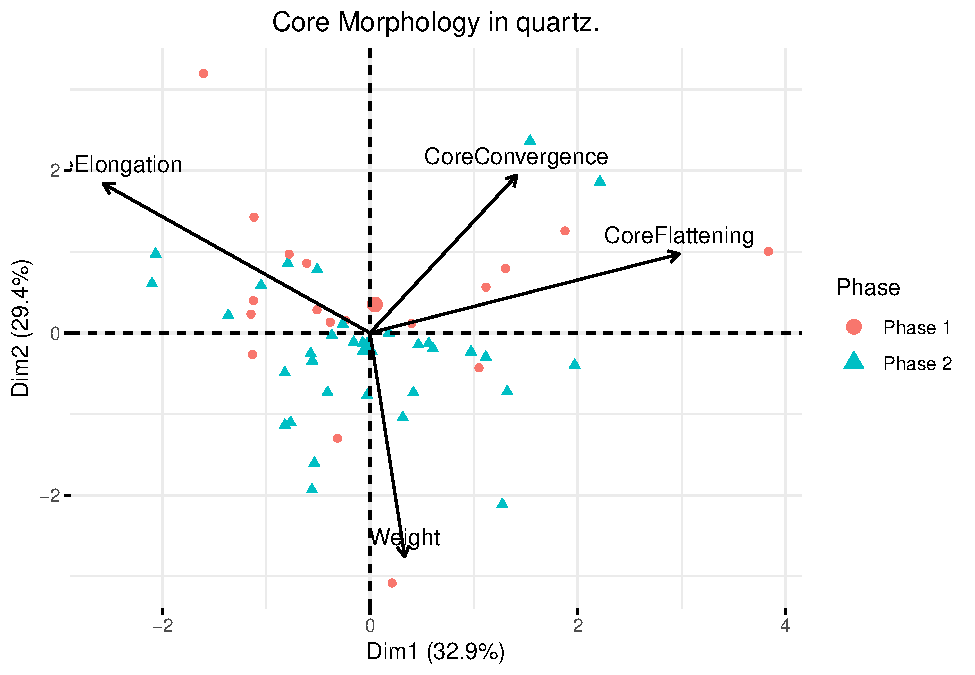
\includegraphics{thesis_files/figure-latex/unnamed-chunk-48-1.pdf}
\caption{\label{fig:unnamed-chunk-48}Variable plot of the first and second components of the Elongated product attributes PCA on chert (EAC).}
\end{figure}
\begin{table}

\caption{\label{tab:unnamed-chunk-49}Positive and negative principal component scores, blank Platform Maintenance PCA (CUC).}
\centering
\begin{tabular}[t]{lc>{\raggedright\arraybackslash}p{3cm}>{\raggedright\arraybackslash}p{3cm}>{\raggedright\arraybackslash}p{3cm}}
\toprule
\multicolumn{1}{c}{\textbf{Dimensions}} & \multicolumn{1}{c}{\textbf{\% variability}} & \multicolumn{1}{>{\centering\arraybackslash}p{3cm}}{\textbf{+}} & \multicolumn{1}{>{\centering\arraybackslash}p{3cm}}{\textbf{-}} & \multicolumn{1}{>{\centering\arraybackslash}p{3cm}}{\textbf{Interpretation}}\\
\midrule
1 & 19.7\% & Hinge termination, Step termination, Irregular profile, 4 or more scar count & Convergent shape, Curved profile, Pointed termination, 3 scar count, 2 scar count & Existence of a group of standardized elongated blanks as opposed to a group of less standardized one.\\
2 & 27.4\% & Hinge termination, Other blankshape, Irregular profile, 4 or more scar count, Overshoot termination, Curved profile, Convergent shape, Pointed termination & Twisted profile, Straight profile, Parallel blankshape, Step termination, Feather termination, 2 scar count & Existence of 3 groups of elongated blanks with unidirectiona scar patterns: 4 or more scars with variable attributes; Convergent shapes, pointed terminations and curved profiles with 3 and 2 scars; Twisted and parallel shapes, with step and feather terminations, with 2 scars.\\
Cumulative \% & 47.1\% &  &  & \\
\bottomrule
\end{tabular}
\end{table}
For elongated attributes on quartz (EAQ), the two main dimensions explain a cumulative 64.7\%, a high value probably result of the small sample.

Dimension 1, which explains most of this variability (40.7\%) shows the correlation on the positive axis of pointed terminations, convergent shapes and curved profiles, other blank shapes, hinged terminations and 3 dorsal scars. On the negative axis, there is the association between step and feather terminations, parallel shapes and straight profiles, with 1 to 2 dorsal scars.
Dimension 2, explaining much less of the variability (24\%) differentiates between a group of blanks with pointed terminations, curved profiles and convergent shapes with 2 dorsal scars, and a group with 3 dorsal scars, hinged terminations, straight profiles and other blank shapes.

These two dimensions seem to, alike chert, create 3 groups of more or less standardized attributes, although the strong association between 3 dorsal scars and hinged termination, as well as with the supplementary variable blade, are probably the result of the small sample.

As such, bladelets are localized right at the centre of both dimensions, since they represent most of the sample. Regarding the other supplementary variables, the U/Lower T group seems closer to the step and feathered terminations, with parallel shapes and straight profiles, with 1 to 2 scars, while the Middle T group is further closer to the group of pointed termination, curved profile and convergent bladelets, which might represent a standardized preference for small elongated blank morphologies in quartz.
\begin{figure}
\centering
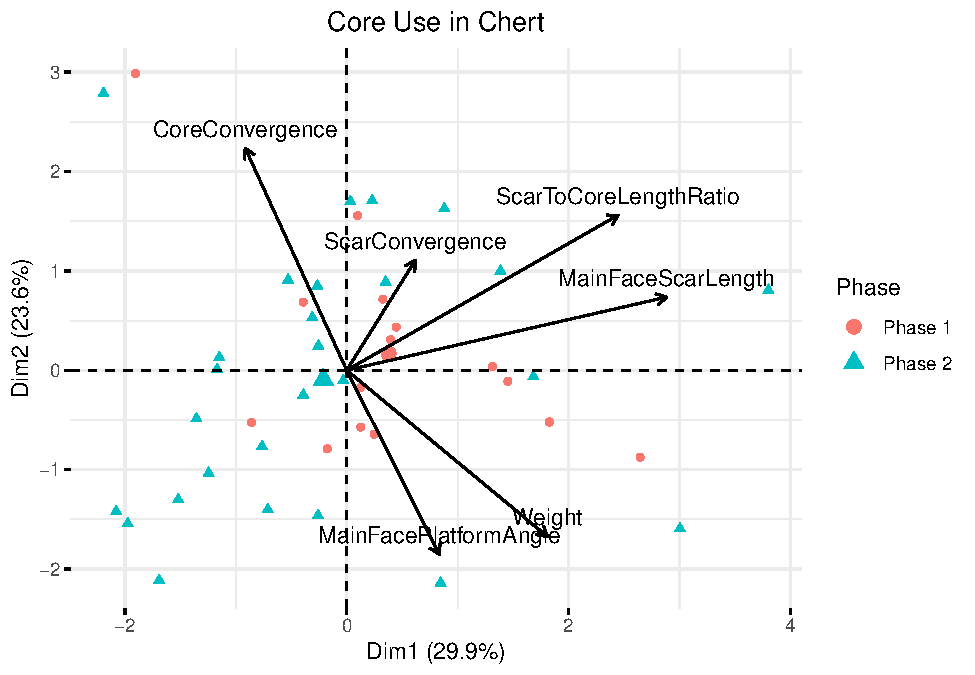
\includegraphics{thesis_files/figure-latex/unnamed-chunk-50-1.pdf}
\caption{\label{fig:unnamed-chunk-50}Variable plot of the first and second components of the Elongated product attributes PCA on quartz (EAQ).}
\end{figure}
\begin{table}

\caption{\label{tab:unnamed-chunk-51}Positive and negative principal component scores, blank Platform Maintenance PCA (CUC).}
\centering
\begin{tabular}[t]{lc>{\raggedright\arraybackslash}p{3cm}>{\raggedright\arraybackslash}p{3cm}>{\raggedright\arraybackslash}p{3cm}}
\toprule
\multicolumn{1}{c}{\textbf{Dimensions}} & \multicolumn{1}{c}{\textbf{\% variability}} & \multicolumn{1}{>{\centering\arraybackslash}p{3cm}}{\textbf{+}} & \multicolumn{1}{>{\centering\arraybackslash}p{3cm}}{\textbf{-}} & \multicolumn{1}{>{\centering\arraybackslash}p{3cm}}{\textbf{Interpretation}}\\
\midrule
1 & 19.7\% & Hinge termination, Step termination, Irregular profile, 4 or more scar count & Convergent shape, Curved profile, Pointed termination, 3 scar count, 2 scar count & Existence of a group of standardized elongated blanks as opposed to a group of less standardized one.\\
2 & 27.4\% & Hinge termination, Other blankshape, Irregular profile, 4 or more scar count, Overshoot termination, Curved profile, Convergent shape, Pointed termination & Twisted profile, Straight profile, Parallel blankshape, Step termination, Feather termination, 2 scar count & Existence of 3 groups of elongated blanks with unidirectiona scar patterns: 4 or more scars with variable attributes; Convergent shapes, pointed terminations and curved profiles with 3 and 2 scars; Twisted and parallel shapes, with step and feather terminations, with 2 scars.\\
Cumulative \% & 47.1\% &  &  & \\
\bottomrule
\end{tabular}
\end{table}
\hypertarget{discussion}{%
\chapter{Discussion}\label{discussion}}

\hypertarget{vale-comprido-technology-1}{%
\section{Vale Comprido technology}\label{vale-comprido-technology-1}}
\begin{verbatim}
Parsed with column specification:
cols(
  Assemblage = col_character(),
  Class = col_character(),
  ElongMean = col_double(),
  ElongSD = col_double(),
  FlatMean = col_double(),
  FlatSD = col_double(),
  PflatMean = col_double(),
  PflatSD = col_double(),
  ConvergentEdges = col_double()
)
\end{verbatim}
Elongation means (\textbackslash ref\{fig: plotsVCelong) show through all of the groups somewhat similar ratios of elongation, with the lowest values appearing in Vale Boi, Vale Comprido -- encosta, for the points, Lapa do Picareiro, Casal do Cepo and Vale Almoinha for the points à face plan, although the differences aren't very significant.

However, the lower elongation values for blades and points from these sites, especially from those with Proto-Solutrean assemblages, might reflect the use of both blades and elongated flakes for the production of the points, thus having a reduction sequence focused on the production of elongated blanks, without the goal of obtaining products with high elongation ratios.

\includegraphics{thesis_files/figure-latex/plotsVCelong-1.pdf}

Regarding flattening (mesial width / thickness, \ref{fig: plotVCflat}) there seems to be a group of sites with smaller values, and thus with blades and points which are less flat: Vale Boi, Vale Comprido -- encosta and Vale de Porcos. This seems to be in concordance with the already established patterns for Proto-Solutrean assemblages, where the production strategies seem to focus thick blanks which are then thinned at the platform. However, it is possible to notice the association between the Lapa do Picareiro blades with other assemblages, with blades and points with higher levels of flattening, thus showing that the Vale Comprido blades show some morphological differences in the flattening ratios from Vale Boi and Vale Comprido -- encosta, both with Proto-Solutrean assemblages.

\includegraphics{thesis_files/figure-latex/plotVCflat-1.pdf}

A similar pattern can be observed for platform flattening means (\ref{fig:plotVCplatflat}), although the differences between Lapa do Picareiro and Vale Boi or Vale Comprido -- Encosta don't seem as obvious. Using this morphological indicator, Casal do Felipe shows the widest differences, with high values for platform flatterning, while the other groups seems rather similar. It is possible to observe, however, that Lapa do Picareiro shows a wide dispersion and variability in terms of platform flattening, comparing, for example, to the low values and low standard deviations from Lapa do Picareiro and Vale Comprido -- Encosta.

\includegraphics{thesis_files/figure-latex/plotVCplatflat-1.pdf}

Regarding the convergence of the edges, figure \ref{fig:plotVCconverge} shows a distinct difference in the percentage of convergence between Lapa do Picareiro, Vale Boi (blades and points) and Vale Comprido -- encosta (blades and points). The blades from these sites show the highest percentages of convergent edges (above 30\%) from all the groups, only surpassed by the values from Vale Comprido points, which reach 50\% in Vale Comprido -- Encosta and more than 60\% in Vale Boi. All the other blades from sites with assemblages belonging to the Solutrean, Gravettian or Aurignacian show values of 20\% or under. This shows not just the already established preference for convergent edges in Vale Comprido points, as well as a high component of convergence in the blank assemblages of these three sites, more specifically, in the blades.

\includegraphics{thesis_files/figure-latex/plotVCconverge-1.pdf}

As such, it seems that the analyzed morphological indicators are good for understanding some variability between the groups and assemblages, as well as distinguishing between blades and points from the same site, which might be useful to understand blade production within the Proto-Solutrean assemblages with the goal of obtaining Vale Comprido points. Although, as seen, all assemblages seem to have a wide variability regarding morphological attributes, which creates difficulties in understanding specific groups based on the means of those indicators. This is especially noticeable with the elongation ratio mean, which didn't show very evident differences between the blade assemblages from the different technocomplexes, although this might also be related to a certain homogeneity in the elongation of blades throughout the Upper Paleolithic.

Regarding the ratios and morphological attribute analysis, Vale Boi seemed to be in concordance with the Vale Comprido -- Encosta values, for both the points and the blanks. The results for the blanks also showed wide similarities with the points, indicating the production of blades is related to the production of the Vale Comprido points.

However, from all of the attributes analyzed, it was the frequency of convergent edges that showed the biggest differences between the Proto-Solutrean assemblages and Lapa do Picareiro against the other assemblages with lesser percentages of convergent edges. This clearly shows that convergence is an important attribute to define the assemblage, its blanks and points.

Despite this similarity, Lapa do Picareiro, especially within the flattening ratios, showed values which were closer to those from the Solutrean assemblages, with flatter blades than those from Vale Boi and Vale Comprido -- Encosta.

These differences, along with the difficulty in identifying Vale Comprido points in the site's Middle T assemblage, for the similarities with the type but lack of defining qualities such as the thickness of the platform or of the blank, and the fairly late chronology attributed to Middle T in Lapa do Picareiro, might represent the nonexistence of a Proto-Solutrean assemblage at the site. Instead, and given the similarities of the Lapa do Picareiro blades with both Proto-Solutrean and Solutrean blades, the assemblage of Middle T might be better explained by a transitional assemblage, chronologically located somewhere in between the Proto-Solutrean and the Middle Solutrean.

\hypertarget{conclusion}{%
\chapter*{Conclusion}\label{conclusion}}
\addcontentsline{toc}{chapter}{Conclusion}

If we don't want Conclusion to have a chapter number next to it, we can add the \texttt{\{-\}} attribute.

\textbf{More info}

And here's some other random info: the first paragraph after a chapter title or section head \emph{shouldn't be} indented, because indents are to tell the reader that you're starting a new paragraph. Since that's obvious after a chapter or section title, proper typesetting doesn't add an indent there.

\hypertarget{references}{%
\chapter*{References}\label{references}}
\addcontentsline{toc}{chapter}{References}

\markboth{References}{References}

\noindent

\setlength{\parindent}{-0.20in}
\setlength{\leftskip}{0.20in}
\setlength{\parskip}{8pt}

\hypertarget{refs}{}
\leavevmode\hypertarget{ref-almeida2000}{}%
Almeida, F. (2000). \emph{The terminal gravettian of portuguese estremadura. Technological variability of the lithic industries.} (PhD thesis).

\leavevmode\hypertarget{ref-andrefsky1994}{}%
Andrefsky, W. (1994). Raw-material availability and the organization of technology. \emph{American Antiquity}, \emph{59}(1), 21--34.

\leavevmode\hypertarget{ref-andrefsky1998}{}%
Andrefsky, W., \& Andrefsky Jr, W. (1998). \emph{Lithics}. Cambridge University Press.

\leavevmode\hypertarget{ref-beardsell2013}{}%
Beardsell, R. J. (2013). \emph{Mass and attribute analysis of the quartz lithic assemblage from the grandfather quarry (HbMd-4), near granville lake, northern manitoba}. University of Manitoba (Canada).

\leavevmode\hypertarget{ref-belmiro2018}{}%
Belmiro, J. (2018). \emph{A ocupação proto-solutrense de vale boi: Novas evidências a partir da indústria lítica} (PhD thesis). Universidade do Algarve, Faro.

\leavevmode\hypertarget{ref-benedettietal2019}{}%
Benedetti, M. M., Haws, J. A., Bicho, N. F., Friedl, L., \& Ellwood, B. B. (2019). Late pleistocene site formation and paleoclimate at lapa do picareiro, portugal. \emph{Geoarchaeology}, \emph{34}(6), 698--726.

\leavevmode\hypertarget{ref-bichoetal2012}{}%
Bicho, N., Cascalheira, J., \& Marreiros, J. (2012). On the (l) edge: The case of vale boi rockshelter (algarve, southern portugal). \emph{Caves in Context. The Economical, Social and Ritual Importance of Caves and Rockshelters}, 65--81.

\leavevmode\hypertarget{ref-bicho2011}{}%
Bicho, N. F., \& Jorge. (2011). \emph{Manual de arqueologia pré-histórica}.

\leavevmode\hypertarget{ref-bicho1992}{}%
Bicho, N. G. F. (1992). Technological change in the final upper paleolithic of rio maior, portuguese estremadura.

\leavevmode\hypertarget{ref-bicho2006}{}%
Bicho, N., Haws, J., \& Hockett, B. (2006). Two sides of the same coin---rocks, bones and site function of picareiro cave, central portugal. \emph{Journal of Anthropological Archaeology}, \emph{25}(4), 485--499.

\leavevmode\hypertarget{ref-brantingham2001}{}%
Brantingham, P. J., \& Kuhn, S. L. (2001). Constraints on levallois core technology: A mathematical model. \emph{Journal of Archaeological Science}, \emph{28}(7), 747--761.

\leavevmode\hypertarget{ref-brezillon1968}{}%
Brézillon, M. N. (1968). La dénomination des objets de pierre taillée.

\leavevmode\hypertarget{ref-carvalho2018}{}%
Carvalho, J. M. (2018). Jointing patterns and tectonic evolution of the maciço calcário estremenho, lusitanian basin, portugal. \emph{Journal of Structural Geology}, \emph{110}, 155--171.

\leavevmode\hypertarget{ref-cascalheira2010}{}%
Cascalheira, J. (2010). \emph{Tecnologia lítica solutrense do abrigo de vale boi (vila do bispo)}. UNIARQ.

\leavevmode\hypertarget{ref-cascalheira2019}{}%
Cascalheira, J. (2019). Territoriality and the organization of technology during the last glacial maximum in southwestern europe. \emph{PloS One}, \emph{14}(12).

\leavevmode\hypertarget{ref-cascalheira2013}{}%
Cascalheira, J. M. M. (2013). A influência mediterrânica nas redes sociais do solutrense final peninsular.

\leavevmode\hypertarget{ref-debenath1994}{}%
Debénath, A., \& Dibble, H. L. (1994). Handbook of paleolithic typology, vol. 1. \emph{University of Pennsylvania, Philadelphia}.

\leavevmode\hypertarget{ref-dibble1997}{}%
Dibble, H. L. (1997). Platform variability and flake morphology: A comparison of experimental and archaeological data and implications for interpreting prehistoric lithic technological strategies. \emph{Lithic Technology}, \emph{22}(2), 150--170.

\leavevmode\hypertarget{ref-dibble2008}{}%
Dibble, H. L. (2008). Non-anthropological approaches to understanding lithic artifact and assemblage variability. \emph{Archaeological Concepts for the Study of the Cultural Past. The University of Utah Press, Salt Lake City}, 85--107.

\leavevmode\hypertarget{ref-dibble2009}{}%
Dibble, H. L., \& Rezek, Z. (2009). Introducing a new experimental design for controlled studies of flake formation: Results for exterior platform angle, platform depth, angle of blow, velocity, and force. \emph{Journal of Archaeological Science}, \emph{36}(9), 1945--1954.

\leavevmode\hypertarget{ref-foley2003}{}%
Foley, R., \& Lahr, M. M. (2003). On stony ground: Lithic technology, human evolution, and the emergence of culture. \emph{Evolutionary Anthropology: Issues, News, and Reviews: Issues, News, and Reviews}, \emph{12}(3), 109--122.

\leavevmode\hypertarget{ref-inizan1999}{}%
Inizan, M.-L., Reduron-Ballinger, M., Roche, H., \& Tixier, J. (1999). Technology and terminology of knapped stone. \emph{Crep, Nanterre}, 189.

\leavevmode\hypertarget{ref-kempson2011}{}%
Kempson, H., \& Wadley, L. (2011). A review of rock studies for archaeologists, and an analysis of dolerite and hornfels from the sibudu area, KwaZulu-natal. \emph{Southern African Humanities}, \emph{23}(1), 87--107.

\leavevmode\hypertarget{ref-leader2017}{}%
Leader, G., Abdolahzadeh, A., Lin, S. C., \& Dibble, H. L. (2017). The effects of platform beveling on flake variation. \emph{Journal of Archaeological Science: Reports}, \emph{16}, 213--223.

\leavevmode\hypertarget{ref-linetal2013}{}%
Lin, S. C., Rezek, Z., Braun, D., \& Dibble, H. L. (2013). On the utility and economization of unretouched flakes: The effects of exterior platform angle and platform depth. \emph{American Antiquity}, \emph{78}(4), 724--745.

\leavevmode\hypertarget{ref-marreiros2009}{}%
Marreiros, J. M. F. (2009). \emph{As primeiras comunidades do homem moderno no algarve ocidental: Caracterização paleotecnológica e paleoetnográfica das comunidades gravetenses e proto-solutrenses de vale boi (algarve, portugal)} (PhD thesis).

\leavevmode\hypertarget{ref-marwick2017}{}%
Marwick, B. (2017). Computational reproducibility in archaeological research: Basic principles and a case study of their implementation. \emph{Journal of Archaeological Method and Theory}, \emph{24}(2), 424--450.

\leavevmode\hypertarget{ref-marwick2018}{}%
Marwick, B., Boettiger, C., \& Mullen, L. (2018). Packaging data analytical work reproducibly using r (and friends). \emph{The American Statistician}, \emph{72}(1), 80--88.

\leavevmode\hypertarget{ref-pereira2013}{}%
Pereira, T., \& Benedetti, M. M. (2013). A model for raw material management as a response to local and global environmental constraints. \emph{Quaternary International}, \emph{318}, 19--32.

\leavevmode\hypertarget{ref-scerri2014}{}%
Scerri, E. M., Groucutt, H. S., Jennings, R. P., \& Petraglia, M. D. (2014). Unexpected technological heterogeneity in northern arabia indicates complex late pleistocene demography at the gateway to asia. \emph{Journal of Human Evolution}, \emph{75}, 125--142.

\leavevmode\hypertarget{ref-sonneville-bordes1956}{}%
Sonneville-Bordes, D., \& Perrot, J. (1956). Lexique typologique du paléolithique supérieur. \emph{Bulletin de La Société Préhistorique Française}, \emph{53}(9), 547--559.

\leavevmode\hypertarget{ref-tixier1963}{}%
Tixier, J. (1963). Typologie de l'Epipaléolithique du maghreb, mémoires du centre de recherches anthropologiques. \emph{Préhistoriques et Ethnographiques d'Alger. Arts et Métiers Graphiques, Paris}.

\leavevmode\hypertarget{ref-tixier1980}{}%
Tixier, J., \& Inizian, M.-L. (1980). Préhistoire de la pierre taillée. 1. Terminologie et technologie.

\leavevmode\hypertarget{ref-tostevin2012}{}%
Tostevin, G. B. (2012). \emph{Seeing lithics: A middle-range theory for testing for cultural transmission in the pleistocene}. American School of Prehistoric Research Monograph Series, Peabody Museum \ldots.

\leavevmode\hypertarget{ref-zilhao1997}{}%
Zilhão, J. (1997). \emph{O paleolítico superior da estremadura portuguesa, volume i}.

\leavevmode\hypertarget{ref-zilhao2013}{}%
Zilhão, J. (2013). Seeing the leaves and not missing the forest: A portuguese perspective of the solutrean. \emph{Pleistocene Foragers on the Iberian Peninsula: Their Culture and Environment. Festschrift in Honour of Gerd-Christian Weniger for His Sixtieth Birthday}, 201--2016.

\leavevmode\hypertarget{ref-zilhaoetal1995}{}%
ZILHÃO, J., \& Aubry, T. (1995). La pointe de vale comprido et les origines du solutréen. \emph{L'Anthropologie}, \emph{99}(1), 125--142.

\appendix

\hypertarget{appendix}{%
\chapter{Appendix}\label{appendix}}
\begin{table}

\caption{\label{tab:unnamed-chunk-52}Basic database attributes recorded. Class conditions represent the classes/artefacts which were considered for each variable, given the programmed system of conditions.}
\centering
\begin{tabular}[t]{>{\raggedright\arraybackslash}p{5cm}>{\raggedright\arraybackslash}p{5cm}}
\toprule
\multicolumn{1}{>{\centering\arraybackslash}p{5cm}}{\textbf{Recorded variables}} & \multicolumn{1}{>{\centering\arraybackslash}p{5cm}}{\textbf{Class conditions}}\\
\midrule
Site & All\\
Area & All\\
Lot & All\\
ID & All\\
Raw material & All\\
\addlinespace
Class & All\\
Cortex presence (\%) & All except shatter and chips\\
Max length & All except fragments, shatter and chips\\
Max width & All except shatter and chips\\
Mesial thickness & All except shatter and chips\\
\addlinespace
Weight & All except chips\\
Type of fracture & Debitage fragments\\
Retouched type & Retouched pieces\\
Alteration & All except shatter and chips\\
Count & Chips\\
\bottomrule
\end{tabular}
\end{table}
\begin{table}

\caption{\label{tab:unnamed-chunk-53}List of all R packages and respective versions used in the thesis.}
\centering
\begin{tabular}[t]{ll}
\toprule
Packages & Used version\\
\midrule
Bchron & 4.3.0\\
readr & 1.3.1\\
dplyr & 0.8.3\\
stringr & 1.4.0\\
tidyr & 1.0.0\\
\addlinespace
knitr & 1.26\\
tab & 3.1.2\\
ggplot2 & 3.2.1\\
FactoMineR & 2.0\\
factoextra & 1.0.6\\
\addlinespace
RcmdrMisc & 2.5.1\\
IDPmisc & 1.1.19\\
forcats & 0.4.0\\
kableExtra & 1.1.0\\
float & 0.2.3\\
\addlinespace
janitor & 1.2.0\\
\bottomrule
\end{tabular}
\end{table}
\begin{landscape}
\begin{longtable}[t]{>{\raggedright\arraybackslash}p{2cm}>{\raggedright\arraybackslash}p{3cm}>{\raggedright\arraybackslash}p{6cm}>{\raggedright\arraybackslash}p{9cm}}
\caption[Lithic analysis Data Dictionary]{\label{tab:unnamed-chunk-54}Data Dictionary with variables considered in the attributes analysis, including measurement units, allowed vallued, definitions and/or references.}\\
\toprule
Variable & Measurement units & Allowed values & Description\\
\midrule
\endfirsthead
\caption[]{\label{tab:unnamed-chunk-54}Data Dictionary with variables considered in the attributes analysis, including measurement units, allowed vallued, definitions and/or references. \textit{(continued)}}\\
\toprule
Variable & Measurement units & Allowed values & Description\\
\midrule
\endhead
\
\endfoot
\bottomrule
\endlastfoot
ID & Numeric & - & ID number assigned to the piece.\\
Raw material & - & Chert, Quartz, Greywacke, Chalcedony, Schist, Silcrete, Dolerite, Other. & Type of raw material of the piece.\\
Quartz quality & - & Coarse, Medium, Fine, Rock crystal. & Type of grain and quality of quartz. Coarse quality: large and visible grains (>0.5 mm). Medium quality: small visible grains. Fine quality: absence of visible grains. Rock crystal: absence of visible grains and transparent coloration.\\
Class & - & Blank, Blank fragment, Retouched piece, Retouched piece fragment, Core, Core fragment, Core preparation product, Core preparation product fragment, Burin spall, Thinn flake, Thinn flake fragment, Anvil, Hammer, Manuport, Shatter, Chip. & Technological class of the piece. According to Andrefsky (1998), Bicho (2011), Debenath and Dibble (1994), Inizan et al. (1999).\\
Core preparation product & - & Crested piece, Core trim, Core tablet, Core front. & Type of core preparation product. According to Inizan et al. (1999).\\
\addlinespace
Retouched piece blank & - & Flake, Elonged blank, Shatter, Other, Indeterminate. & Type of retouched piece blank. According to Inizan et al (1999).\\
Piece completeness & - & Proximal, Distal, Other. & Part of the piece that is present. Proximal refers to the part which has a bulb and a striking platform; distal is the end of the piece; other refers to mesial.\\
Cortex & - & 0\%, 1-30\%, 31-60\%, 61-99\%, 100\%. & Percentage of cortex presence in the dorsal face of the piece. According to Andrefsky (2005, pp. 104-105) and Bicho (2011).\\
Cortex location & - & Proximal, Distal, Mesial, Left lateral, Right lateral, Proximal left lateral, Proximal right lateral, Distal left lateral, Distal right lateral, Mesial left lateral, Mesial right lateral. & Location of cortex in the dorsal surface of the piece.\\
Cortex type & - & Cobble, Outcrop, Indeterminate. & Type of cortex present on the piece. Cobble refers to rounded clasts of rock; Outcrop is an exposed bedrock or superficial deposits.\\
\addlinespace
Platform type & - & Plain, Dihedral, Faceted, Punctiform, Linear, Winged, Removed, Crushed, Other. & Type of platform. According to Inizan et al (1999, pp. 136).\\
Platform cortex & - & No, Yes complete, Yes partial. & Presence of cortex on the piece’s platform.\\
Lipping & - & No, Yes. & Presence of a lip on the piece. According to Inizan et al (1999, pp. 144).\\
Blank shape & - & Parallel, Convergent, Divergent, Biconvex, Irregular, Circular, Dejete, Other. & Type of blank shape. According to Almeida (2000, pp. 107).\\
Cross section & - & Triangular, Trapezoidal, Quadrangular, Irregular, Lenticular, Other. & Type of cross section of the piece. According to Scerri et al (2015, pp. 19).\\
\addlinespace
Blank tip & - & Feather, Hinge, Step, Overshoot, Pointed. & Type of blank tip. According to Almeida (2000, pp. 106).\\
Profile & - & Straight, Curved, Twisted, Irregular. & Type of blank profile. According to Almeida (2000, pp. 106).\\
Scar count & Numeric &  & Count of dorsal flake scars over 5 mm. According to Andrefsky (2005, pp. 106).\\
Scar pattern & - & Unidirectional, Bidirectional, Crossed, Sub-centripedal, Centripedal, Other. & Type of scar pattern on the dorsal surface of the piece. According to Scerri et al (2015, pp. 19).\\
Thickness & In mm & - & Measurement of piece maximum thickness.\\
\addlinespace
Max width & In mm & - & Measurement of piece maximum width.\\
Proximal width & In mm & - & Measurement of piece proximal width.\\
Mesial width & In mm & - & Measurement of piece mesial width.\\
Distal width & In mm & - & Measurement of piece distal width.\\
Length & In mm & - & Measurement of piece central length according to the technological axis.\\
\addlinespace
Platform thickness & In mm & - & Measurement of platform central thickness.\\
Platform width & In mm & - & Measurement of platform central width.\\
Weight & In grams & - & Weight measurement of piece.\\
Exterior platform angle & In degrees & - & Measurement of the angle between the platform and the dorsal surface of the piece. According to Dibble (1997).\\
Core type & - & Single platform, Single prismatic, Single pyramidal, Two single platforms, Opposed, Opposed twisted, Other opposed, Orthogonal, Inform, Bipolar, Globular, Centripedal, Discoidal, Levallois, Chopper, Tested, Other. & Type of core. According to Zilhao (1997, pp. 17).\\
\addlinespace
Core Cross Section & - & Circular, Triangular, Quadrangular, Irregular. & Type of core cross section.\\
Number of core faces & - & One, Two, Three, Four, More than four. & Count of core debitage surfaces.\\
Core platform & - & Plain, Dihedral, Faceted, Cortical, Crushed, Other. & Type of core platform. According to Inizan et al (1999, pp. 136).\\
Main face cortex & - & 0\%, 1-30\%, 31-60\%, 61-99\%. & Percentage of cortex of the core’s main face. Main face refers to the debitage surface with most scars.\\
Main face scar count & Numeric & - & Count of scars over 5 mm in the main face of the core.\\
\addlinespace
Main face scar direction & - & Unidirectional, Bidirectional opposed, Bidirectional alternate, Crossed, Sub-centripedal, Centripedal, Other. & Direction of scars in the main face of the core. According to Scerri et al (2015, pp. 19).\\
Main face aris orientation & - & Parallel, Convergent, Indeterminate. & Orientation of main face aris.\\
Main face scar length & In mm & - & Central length measurement of the last scar, over 5 mm, in the main face of the core.\\
Main face scar width & In mm & - & Maximum width measurement of the last scar, over 5 mm, in the main face of the core.\\
Main face platform angle & In degrees & - & Measurement of the angle between the platform and the main face of the core.\\
\addlinespace
Main face core use & - & Flakes, Blades, Bladelets, Points, Mixed. & Type of products extracted from the main face of the core. Distinction of blade and bladelet according to Tixier (1963).\\
Alteration & - & None, Patinated, Concretion, Fire, Mix. & Type of alteration of the piece. Patina refers to a layer covering the surface of a piece; concretion is a mass of mineral formed around a nucleus.\\
Fire & - & Burned, Rubefact, Heat treatment. & Type of fire alteration to the piece. According to Inizan et al (1999, pp. 24).\\
Retouched piece typology & - & - & Retouched piece typology as defined by Sonneville-Bordes and Perrot (1956), adapted by Zilhao (1997) for the Portuguese Estremadura.\\
Chip quantity & Numeric & - & Count of chips. According to Andrefsky (2005, pp. 12).\\
\addlinespace
Other notes & - & - & \\*
\end{longtable}
\end{landscape}
\begin{figure}
\includegraphics[width=1\linewidth]{figure/thin_section} \caption{Dolerite thin section under seen through a polarized microscope.}\label{fig:unnamed-chunk-55}
\end{figure}
\begin{figure}
\includegraphics[width=1\linewidth]{figure/dolerite_sample} \caption{Location of recovered dolerite sample (yellow) comparatively to Vale Boi (orange).}\label{fig:unnamed-chunk-56}
\end{figure}
\begin{longtable}[t]{lllll}
\caption{\label{tab:unnamed-chunk-57}Phase 1 Core attributes (frequencies) and platform measurements (mean and standard deviation) table.}\\
\toprule
\multicolumn{1}{c}{\textbf{Tecnological attributes}} & \multicolumn{1}{c}{\textbf{Quartz}} & \multicolumn{1}{c}{\textbf{Chert}} & \multicolumn{1}{c}{\textbf{Greywacke}} & \multicolumn{1}{c}{\textbf{Other}}\\
\midrule
CoreType, n (\%) &  &  &  & \\
Opposed & 1 (6.7) & 0 (0.0) & 0 (0.0) & 0 (0.0)\\
SinglePlat & 11 (73.3) & 8 (50.0) & 2 (100.0) & 0 (0.0)\\
SinglePrismatic & 2 (13.3) & 6 (37.5) & 0 (0.0) & 0 (0.0)\\
SinglePyramidal & 1 (6.7) & 1 (6.2) & 0 (0.0) & 1 (100.0)\\
\addlinespace
TwoSinglePlat & 0 (0.0) & 1 (6.2) & 0 (0.0) & 0 (0.0)\\
NumberCoreFaces, n (\%) &  &  &  & \\
Four & 3 (20.0) & 0 (0.0) & 0 (0.0) & 0 (0.0)\\
MoreThanFour & 0 (0.0) & 2 (12.5) & 0 (0.0) & 0 (0.0)\\
One & 4 (26.7) & 7 (43.8) & 2 (100.0) & 1 (100.0)\\
\addlinespace
Three & 3 (20.0) & 3 (18.8) & 0 (0.0) & 0 (0.0)\\
Two & 5 (33.3) & 4 (25.0) & 0 (0.0) & 0 (0.0)\\
CorePlatform, n (\%) &  &  &  & \\
Cortical & 3 (20.0) & 1 (6.2) & 2 (100.0) & 0 (0.0)\\
Faceted & 1 (6.7) & 1 (6.2) & 0 (0.0) & 0 (0.0)\\
\addlinespace
Plain & 11 (73.3) & 14 (87.5) & 0 (0.0) & 1 (100.0)\\
PlatformWidth, M (SD) & 33.2 (14.2) & 29.3 (11.6) & 79.8 (0.8) & 35.6 (NA)\\
PlatformThickness, M (SD) & 23.2 (12.0) & 21.6 (6.9) & 45.4 (4.8) & 23.9 (NA)\\
MainFaceCoreUse, n (\%) &  &  &  & \\
Bladelets & 1 (6.7) & 2 (12.5) & 0 (0.0) & 0 (0.0)\\
\addlinespace
Blades & 1 (6.7) & 4 (25.0) & 0 (0.0) & 0 (0.0)\\
Flakes & 13 (86.7) & 10 (62.5) & 2 (100.0) & 0 (0.0)\\
Mixed & 0 (0.0) & 0 (0.0) & 0 (0.0) & 1 (100.0)\\
MainFacePlatformAngle, M (SD) & 81.7 (10.7) & 80.8 (15.9) & 84.7 (25.9) & 83.1 (NA)\\
\bottomrule
\end{longtable}
\begin{longtable}[t]{llll}
\caption{\label{tab:unnamed-chunk-58}Phase 2 Core attributes (frequencies) and platform measurements (mean and standard deviation) table.}\\
\toprule
\multicolumn{1}{c}{\textbf{Tecnological attributes}} & \multicolumn{1}{c}{\textbf{Quartz}} & \multicolumn{1}{c}{\textbf{Chert}} & \multicolumn{1}{c}{\textbf{Other}}\\
\midrule
CoreType, n (\%) &  &  & \\
Opposed & 0 (0.0) & 3 (11.1) & 0 (0.0)\\
Other & 0 (0.0) & 3 (11.1) & 0 (0.0)\\
SinglePlat & 21 (72.4) & 9 (33.3) & 2 (100.0)\\
SinglePrismatic & 6 (20.7) & 3 (11.1) & 0 (0.0)\\
\addlinespace
SinglePyramidal & 1 (3.4) & 4 (14.8) & 0 (0.0)\\
TwoSinglePlat & 1 (3.4) & 5 (18.5) & 0 (0.0)\\
NumberCoreFaces, n (\%) &  &  & \\
Four & 1 (3.4) & 2 (7.4) & 0 (0.0)\\
MoreThanFour & 0 (0.0) & 0 (0.0) & 0 (0.0)\\
\addlinespace
One & 14 (48.3) & 12 (44.4) & 2 (100.0)\\
Three & 2 (6.9) & 4 (14.8) & 0 (0.0)\\
Two & 12 (41.4) & 9 (33.3) & 0 (0.0)\\
CorePlatform, n (\%) &  &  & \\
Cortical & 9 (31.0) & 1 (3.7) & 1 (50.0)\\
\addlinespace
Crushed & 1 (3.4) & 2 (7.4) & 0 (0.0)\\
Dihedral & 0 (0.0) & 2 (7.4) & 0 (0.0)\\
Faceted & 1 (3.4) & 5 (18.5) & 0 (0.0)\\
Other & 0 (0.0) & 2 (7.4) & 0 (0.0)\\
Plain & 18 (62.1) & 15 (55.6) & 1 (50.0)\\
\addlinespace
PlatformWidth, M (SD) & 34.5 (13.5) & 26.8 (9.8) & 43.1 (16.7)\\
PlatformThickness, M (SD) & 26.8 (10.8) & 19.4 (10.6) & 19.5 (2.5)\\
MainFaceCoreUse, n (\%) &  &  & \\
Bladelets & 3 (10.3) & 3 (11.1) & 0 (0.0)\\
Blades & 2 (6.9) & 4 (14.8) & 0 (0.0)\\
\addlinespace
Flakes & 20 (69.0) & 16 (59.3) & 2 (100.0)\\
Mixed & 4 (13.8) & 4 (14.8) & 0 (0.0)\\
MainFacePlatformAngle, M (SD) & 77.6 (12.8) & 81.2 (20.2) & 89.8 (18.3)\\
\bottomrule
\end{longtable}
\begin{table}[!h]

\caption{\label{tab:unnamed-chunk-59}Phase 1 Core measurements (width, length and thickness) with mean and standard deviation values.}
\centering
\begin{tabular}[t]{lllll}
\toprule
\multicolumn{1}{c}{\textbf{Core metrics}} & \multicolumn{1}{c}{\textbf{Quartz}} & \multicolumn{1}{c}{\textbf{Chert}} & \multicolumn{1}{c}{\textbf{Greywacke}} & \multicolumn{1}{c}{\textbf{Other}}\\
\midrule
MaxWidth, M (SD) & 33.1 (13.7) & 33.7 (15.9) & 65.0 (25.1) & 44.9 (NA)\\
Length, M (SD) & 26.6 (7.2) & 29.1 (12.9) & 32.4 (10.5) & 36.3 (NA)\\
Thickness, M (SD) & 23.4 (11.8) & 22.8 (6.6) & 36.1 (8.0) & 32.6 (NA)\\
\bottomrule
\end{tabular}
\end{table}
\begin{table}[!h]

\caption{\label{tab:unnamed-chunk-60}Phase 2 Core measurements (width, length and thickness) with mean and standard deviation values.}
\centering
\begin{tabular}[t]{lllll}
\toprule
\multicolumn{1}{c}{\textbf{Core metrics}} & \multicolumn{1}{c}{\textbf{Quartz}} & \multicolumn{1}{c}{\textbf{Chert}} & \multicolumn{1}{c}{\textbf{Greywacke}} & \multicolumn{1}{c}{\textbf{Other}}\\
\midrule
MaxWidth, M (SD) & 35.7 (13.7) & 29.0 (8.9) & 16.2 (NA) & 53.4 (6.4)\\
Length, M (SD) & 25.8 (10.2) & 26.5 (8.9) & 33.9 (NA) & 36.9 (26.3)\\
Thickness, M (SD) & 27.0 (9.9) & 21.6 (10.0) & 18.1 (NA) & 32.6 (9.4)\\
\bottomrule
\end{tabular}
\end{table}
\begin{longtable}[t]{>{\raggedright\arraybackslash}p{1cm}>{\raggedright\arraybackslash}p{1cm}>{\raggedright\arraybackslash}p{1cm}>{\raggedright\arraybackslash}p{1cm}>{\raggedright\arraybackslash}p{1cm}>{\raggedright\arraybackslash}p{1cm}>{\raggedright\arraybackslash}p{1cm}}
\caption{\label{tab:unnamed-chunk-61}Phase 1 Blank attributes (frequencies) and platform measurements (mean and standard deviation) table.}\\
\toprule
\multicolumn{1}{c}{\textbf{Attributes}} & \multicolumn{1}{c}{\textbf{Quartz}} & \multicolumn{1}{c}{\textbf{Chert}} & \multicolumn{1}{c}{\textbf{Greywacke}} & \multicolumn{1}{c}{\textbf{Dolerite}} & \multicolumn{1}{c}{\textbf{Chalcedony}} & \multicolumn{1}{c}{\textbf{Other}}\\
\midrule
CrossSection, n (\%) &  &  &  &  &  & \\
Irregular & 118 (49.8) & 50 (35.7) & 12 (31.6) & 1 (33.3) & 2 (40.0) & 2 (50.0)\\
Lenticular & 24 (10.1) & 32 (22.9) & 7 (18.4) & 0 (0.0) & 0 (0.0) & 1 (25.0)\\
Other & 5 (2.1) & 3 (2.1) & 0 (0.0) & 0 (0.0) & 0 (0.0) & 0 (0.0)\\
Quadrangular & 13 (5.5) & 3 (2.1) & 3 (7.9) & 0 (0.0) & 0 (0.0) & 1 (25.0)\\
\addlinespace
Trapezoidal & 11 (4.6) & 5 (3.6) & 4 (10.5) & 0 (0.0) & 0 (0.0) & 0 (0.0)\\
Triangular & 66 (27.8) & 47 (33.6) & 12 (31.6) & 2 (66.7) & 3 (60.0) & 0 (0.0)\\
BlankShape, n (\%) &  &  &  &  &  & \\
Circular & 9 (3.8) & 4 (2.9) & 1 (2.6) & 0 (0.0) & 0 (0.0) & 1 (25.0)\\
Convergent & 60 (25.3) & 20 (14.3) & 8 (21.1) & 1 (33.3) & 1 (20.0) & 0 (0.0)\\
\addlinespace
Dejete & 4 (1.7) & 5 (3.6) & 0 (0.0) & 0 (0.0) & 0 (0.0) & 0 (0.0)\\
Divergent & 9 (3.8) & 19 (13.6) & 2 (5.3) & 0 (0.0) & 1 (20.0) & 1 (25.0)\\
Irregular & 108 (45.6) & 68 (48.6) & 20 (52.6) & 0 (0.0) & 3 (60.0) & 0 (0.0)\\
Parallel & 47 (19.8) & 24 (17.1) & 7 (18.4) & 2 (66.7) & 0 (0.0) & 2 (50.0)\\
Profile, n (\%) &  &  &  &  &  & \\
\addlinespace
Curved & 32 (13.5) & 62 (44.3) & 7 (18.4) & 1 (33.3) & 0 (0.0) & 3 (75.0)\\
Irregular & 47 (19.8) & 14 (10.0) & 9 (23.7) & 0 (0.0) & 2 (40.0) & 0 (0.0)\\
Straight & 154 (65.0) & 60 (42.9) & 21 (55.3) & 2 (66.7) & 2 (40.0) & 1 (25.0)\\
Twisted & 4 (1.7) & 4 (2.9) & 1 (2.6) & 0 (0.0) & 1 (20.0) & 0 (0.0)\\
BlankTip, n (\%) &  &  &  &  &  & \\
\addlinespace
Feather & 65 (27.4) & 68 (48.6) & 15 (39.5) & 0 (0.0) & 2 (40.0) & 1 (25.0)\\
Hinge & 107 (45.1) & 28 (20.0) & 10 (26.3) & 2 (66.7) & 1 (20.0) & 1 (25.0)\\
Overshoot & 1 (0.4) & 4 (2.9) & 0 (0.0) & 0 (0.0) & 0 (0.0) & 0 (0.0)\\
Pointed & 31 (13.1) & 9 (6.4) & 2 (5.3) & 0 (0.0) & 0 (0.0) & 0 (0.0)\\
Step & 33 (13.9) & 31 (22.1) & 11 (28.9) & 1 (33.3) & 2 (40.0) & 2 (50.0)\\
\addlinespace
PlatformType, n (\%) &  &  &  &  &  & \\
Crushed & 79 (33.3) & 21 (15.0) & 2 (5.3) & 1 (33.3) & 2 (40.0) & 0 (0.0)\\
Dihedral & 2 (0.8) & 6 (4.3) & 0 (0.0) & 0 (0.0) & 0 (0.0) & 0 (0.0)\\
Faceted & 0 (0.0) & 2 (1.4) & 0 (0.0) & 0 (0.0) & 0 (0.0) & 0 (0.0)\\
Linear & 0 (0.0) & 5 (3.6) & 1 (2.6) & 0 (0.0) & 0 (0.0) & 0 (0.0)\\
\addlinespace
Other & 2 (0.8) & 0 (0.0) & 1 (2.6) & 0 (0.0) & 0 (0.0) & 0 (0.0)\\
Plain & 154 (65.0) & 97 (69.3) & 34 (89.5) & 2 (66.7) & 3 (60.0) & 3 (75.0)\\
Winged & 0 (0.0) & 9 (6.4) & 0 (0.0) & 0 (0.0) & 0 (0.0) & 1 (25.0)\\
PlatformCortex, n (\%) &  &  &  &  &  & \\
No & 233 (98.3) & 121 (86.4) & 34 (89.5) & 3 (100.0) & 5 (100.0) & 4 (100.0)\\
\addlinespace
YesComplete & 3 (1.3) & 15 (10.7) & 4 (10.5) & 0 (0.0) & 0 (0.0) & 0 (0.0)\\
YesPartial & 1 (0.4) & 4 (2.9) & 0 (0.0) & 0 (0.0) & 0 (0.0) & 0 (0.0)\\
PlatformWidth, M (SD) & 15.2 (7.4) & 10.9 (5.6) & 21.9 (12.1) & 11.1 (3.4) & 8.8 (4.7) & 12.6 (5.1)\\
PlatformThickness, M (SD) & 7.84 (4.20) & 4.58 (2.44) & 9.84 (5.07) & 4.86 (1.17) & 4.45 (2.87) & 5.27 (3.46)\\
ScarCount, n (\%) &  &  &  &  &  & \\
\addlinespace
0 & 2 (0.8) & 2 (1.4) & 2 (5.3) & 0 (0.0) & 0 (0.0) & 0 (0.0)\\
1 & 89 (37.6) & 39 (27.9) & 17 (44.7) & 1 (33.3) & 1 (20.0) & 3 (75.0)\\
2 & 100 (42.2) & 49 (35.0) & 11 (28.9) & 1 (33.3) & 3 (60.0) & 1 (25.0)\\
3 & 38 (16.0) & 32 (22.9) & 4 (10.5) & 1 (33.3) & 0 (0.0) & 0 (0.0)\\
4 & 7 (3.0) & 12 (8.6) & 3 (7.9) & 0 (0.0) & 1 (20.0) & 0 (0.0)\\
\addlinespace
5 & 0 (0.0) & 5 (3.6) & 0 (0.0) & 0 (0.0) & 0 (0.0) & 0 (0.0)\\
6 & 1 (0.4) & 0 (0.0) & 0 (0.0) & 0 (0.0) & 0 (0.0) & 0 (0.0)\\
7 & 0 (0.0) & 1 (0.7) & 0 (0.0) & 0 (0.0) & 0 (0.0) & 0 (0.0)\\
8 & 0 (0.0) & 0 (0.0) & 1 (2.6) & 0 (0.0) & 0 (0.0) & 0 (0.0)\\
ScarPattern, n (\%) &  &  &  &  &  & \\
\addlinespace
Bidirectional & 3 (1.3) & 13 (9.3) & 2 (5.3) & 0 (0.0) & 0 (0.0) & 0 (0.0)\\
Centripetal & 0 (0.0) & 0 (0.0) & 1 (2.6) & 0 (0.0) & 1 (20.0) & 0 (0.0)\\
Crossed & 1 (0.4) & 1 (0.7) & 0 (0.0) & 0 (0.0) & 0 (0.0) & 0 (0.0)\\
None & 2 (0.8) & 2 (1.4) & 2 (5.3) & 0 (0.0) & 0 (0.0) & 0 (0.0)\\
Other & 0 (0.0) & 2 (1.4) & 0 (0.0) & 0 (0.0) & 0 (0.0) & 0 (0.0)\\
\addlinespace
Unidirectional & 231 (97.5) & 122 (87.1) & 33 (86.8) & 3 (100.0) & 4 (80.0) & 4 (100.0)\\
\bottomrule
\end{longtable}
\begin{longtable}[t]{>{\raggedright\arraybackslash}p{1cm}>{\raggedright\arraybackslash}p{1cm}>{\raggedright\arraybackslash}p{1cm}>{\raggedright\arraybackslash}p{1cm}>{\raggedright\arraybackslash}p{1cm}>{\raggedright\arraybackslash}p{1cm}>{\raggedright\arraybackslash}p{1cm}}
\caption{\label{tab:unnamed-chunk-62}Phase 2 Blank attributes (frequencies) and platform measurements (mean and standard deviation) table.}\\
\toprule
\multicolumn{1}{c}{\textbf{Attributes}} & \multicolumn{1}{c}{\textbf{Quartz}} & \multicolumn{1}{c}{\textbf{Chert}} & \multicolumn{1}{c}{\textbf{Greywacke}} & \multicolumn{1}{c}{\textbf{Dolerite}} & \multicolumn{1}{c}{\textbf{Chalcedony}} & \multicolumn{1}{c}{\textbf{Other}}\\
\midrule
CrossSection, n (\%) &  &  &  &  &  & \\
Irregular & 191 (49.4) & 121 (36.4) & 30 (39.5) & 5 (38.5) & 6 (42.9) & 1 (16.7)\\
Lenticular & 44 (11.4) & 45 (13.6) & 19 (25.0) & 1 (7.7) & 2 (14.3) & 1 (16.7)\\
Other & 6 (1.6) & 7 (2.1) & 2 (2.6) & 0 (0.0) & 0 (0.0) & 0 (0.0)\\
Quadrangular & 14 (3.6) & 4 (1.2) & 1 (1.3) & 0 (0.0) & 0 (0.0) & 0 (0.0)\\
\addlinespace
Trapezoidal & 12 (3.1) & 24 (7.2) & 2 (2.6) & 3 (23.1) & 2 (14.3) & 0 (0.0)\\
Triangular & 120 (31.0) & 131 (39.5) & 22 (28.9) & 4 (30.8) & 4 (28.6) & 4 (66.7)\\
BlankShape, n (\%) &  &  &  &  &  & \\
Circular & 16 (4.1) & 7 (2.1) & 2 (2.6) & 1 (7.7) & 1 (7.1) & 0 (0.0)\\
Convergent & 113 (29.2) & 67 (20.2) & 13 (17.1) & 1 (7.7) & 3 (21.4) & 0 (0.0)\\
\addlinespace
Dejete & 6 (1.6) & 15 (4.5) & 8 (10.5) & 0 (0.0) & 0 (0.0) & 0 (0.0)\\
Divergent & 32 (8.3) & 55 (16.6) & 6 (7.9) & 2 (15.4) & 2 (14.3) & 0 (0.0)\\
Irregular & 111 (28.7) & 118 (35.5) & 41 (53.9) & 9 (69.2) & 4 (28.6) & 5 (83.3)\\
Other & 1 (0.3) & 0 (0.0) & 0 (0.0) & 0 (0.0) & 0 (0.0) & 0 (0.0)\\
Parallel & 108 (27.9) & 70 (21.1) & 6 (7.9) & 0 (0.0) & 4 (28.6) & 1 (16.7)\\
\addlinespace
Profile, n (\%) &  &  &  &  &  & \\
Curved & 75 (19.4) & 146 (44.0) & 24 (31.6) & 6 (46.2) & 6 (42.9) & 4 (66.7)\\
Irregular & 60 (15.5) & 24 (7.2) & 10 (13.2) & 1 (7.7) & 2 (14.3) & 0 (0.0)\\
Straight & 246 (63.6) & 157 (47.3) & 42 (55.3) & 5 (38.5) & 6 (42.9) & 2 (33.3)\\
Twisted & 6 (1.6) & 5 (1.5) & 0 (0.0) & 1 (7.7) & 0 (0.0) & 0 (0.0)\\
\addlinespace
BlankTip, n (\%) &  &  &  &  &  & \\
Feather & 76 (19.6) & 139 (41.9) & 34 (44.7) & 6 (46.2) & 9 (64.3) & 3 (50.0)\\
Hinge & 220 (56.8) & 64 (19.3) & 22 (28.9) & 2 (15.4) & 1 (7.1) & 2 (33.3)\\
Overshoot & 3 (0.8) & 8 (2.4) & 0 (0.0) & 0 (0.0) & 0 (0.0) & 0 (0.0)\\
Pointed & 49 (12.7) & 29 (8.7) & 8 (10.5) & 0 (0.0) & 2 (14.3) & 0 (0.0)\\
\addlinespace
Step & 39 (10.1) & 92 (27.7) & 12 (15.8) & 5 (38.5) & 2 (14.3) & 1 (16.7)\\
PlatformType, n (\%) &  &  &  &  &  & \\
Crushed & 139 (35.9) & 53 (16.0) & 5 (6.6) & 2 (15.4) & 2 (14.3) & 0 (0.0)\\
Dihedral & 2 (0.5) & 23 (6.9) & 1 (1.3) & 1 (7.7) & 3 (21.4) & 0 (0.0)\\
Faceted & 0 (0.0) & 8 (2.4) & 1 (1.3) & 0 (0.0) & 0 (0.0) & 0 (0.0)\\
\addlinespace
Linear & 2 (0.5) & 10 (3.0) & 3 (3.9) & 1 (7.7) & 0 (0.0) & 0 (0.0)\\
Other & 0 (0.0) & 1 (0.3) & 0 (0.0) & 0 (0.0) & 0 (0.0) & 0 (0.0)\\
Plain & 243 (62.8) & 217 (65.4) & 66 (86.8) & 9 (69.2) & 7 (50.0) & 6 (100.0)\\
Winged & 1 (0.3) & 20 (6.0) & 0 (0.0) & 0 (0.0) & 2 (14.3) & 0 (0.0)\\
PlatformCortex, n (\%) &  &  &  &  &  & \\
\addlinespace
No & 377 (97.4) & 270 (81.3) & 65 (85.5) & 12 (92.3) & 14 (100.0) & 5 (83.3)\\
YesComplete & 6 (1.6) & 35 (10.5) & 11 (14.5) & 1 (7.7) & 0 (0.0) & 1 (16.7)\\
YesPartial & 4 (1.0) & 27 (8.1) & 0 (0.0) & 0 (0.0) & 0 (0.0) & 0 (0.0)\\
PlatformWidth, M (SD) & 15.3 (7.7) & 11.4 (5.1) & 20.3 (9.3) & 17.7 (10.5) & 13.3 (4.7) & 16.4 (5.5)\\
PlatformThickness, M (SD) & 7.56 (3.71) & 4.93 (2.74) & 7.83 (4.24) & 5.45 (3.09) & 5.43 (2.11) & 8.23 (3.10)\\
\addlinespace
ScarCount, n (\%) &  &  &  &  &  & \\
0 & 5 (1.3) & 16 (4.8) & 2 (2.6) & 0 (0.0) & 0 (0.0) & 1 (16.7)\\
1 & 156 (40.3) & 78 (23.5) & 25 (32.9) & 3 (23.1) & 5 (35.7) & 0 (0.0)\\
2 & 160 (41.3) & 125 (37.7) & 30 (39.5) & 6 (46.2) & 4 (28.6) & 3 (50.0)\\
3 & 60 (15.5) & 79 (23.8) & 14 (18.4) & 4 (30.8) & 2 (14.3) & 2 (33.3)\\
\addlinespace
4 & 5 (1.3) & 26 (7.8) & 2 (2.6) & 0 (0.0) & 1 (7.1) & 0 (0.0)\\
5 & 1 (0.3) & 5 (1.5) & 2 (2.6) & 0 (0.0) & 0 (0.0) & 0 (0.0)\\
6 & 0 (0.0) & 3 (0.9) & 1 (1.3) & 0 (0.0) & 1 (7.1) & 0 (0.0)\\
8 & 0 (0.0) & 0 (0.0) & 0 (0.0) & 0 (0.0) & 1 (7.1) & 0 (0.0)\\
ScarPattern, n (\%) &  &  &  &  &  & \\
\addlinespace
Bidirectional & 11 (2.8) & 26 (7.8) & 2 (2.6) & 2 (15.4) & 2 (14.3) & 0 (0.0)\\
Centripetal & 1 (0.3) & 5 (1.5) & 3 (3.9) & 1 (7.7) & 0 (0.0) & 0 (0.0)\\
None & 5 (1.3) & 16 (4.8) & 2 (2.6) & 0 (0.0) & 0 (0.0) & 1 (16.7)\\
Other & 2 (0.5) & 1 (0.3) & 2 (2.6) & 0 (0.0) & 0 (0.0) & 0 (0.0)\\
Unidirectional & 368 (95.1) & 284 (85.5) & 67 (88.2) & 10 (76.9) & 12 (85.7) & 5 (83.3)\\
\bottomrule
\end{longtable}
\begin{table}[!h]

\caption{\label{tab:unnamed-chunk-63}Phase 1 Blank measurements (width, length and thickness) with mean and standard deviation values.}
\centering
\resizebox{\linewidth}{!}{
\begin{tabular}[t]{lllllll}
\toprule
\multicolumn{1}{c}{\textbf{Measurements}} & \multicolumn{1}{c}{\textbf{Quartz}} & \multicolumn{1}{c}{\textbf{Chert}} & \multicolumn{1}{c}{\textbf{Greywacke}} & \multicolumn{1}{c}{\textbf{Dolerite}} & \multicolumn{1}{c}{\textbf{Chalcedony}} & \multicolumn{1}{c}{\textbf{Other}}\\
\midrule
MaxWidth, M (SD) & 19.9 (7.2) & 18.0 (6.6) & 31.6 (16.0) & 15.6 (4.6) & 15.6 (5.3) & 23.2 (3.6)\\
Length, M (SD) & 23.0 (7.6) & 19.4 (7.3) & 32.9 (13.5) & 18.0 (5.0) & 20.6 (10.2) & 26.3 (7.4)\\
Thickness, M (SD) & 8.9 (3.8) & 5.5 (2.6) & 10.9 (6.0) & 5.5 (1.3) & 6.6 (3.5) & 6.6 (3.0)\\
\bottomrule
\end{tabular}}
\end{table}
\begin{table}[!h]

\caption{\label{tab:unnamed-chunk-64}Phase 2 Blank measurements (width, length and thickness) with mean and standard deviation values.}
\centering
\resizebox{\linewidth}{!}{
\begin{tabular}[t]{lllllll}
\toprule
\multicolumn{1}{c}{\textbf{Measurements}} & \multicolumn{1}{c}{\textbf{Quartz}} & \multicolumn{1}{c}{\textbf{Chert}} & \multicolumn{1}{c}{\textbf{Greywacke}} & \multicolumn{1}{c}{\textbf{Dolerite}} & \multicolumn{1}{c}{\textbf{Chalcedony}} & \multicolumn{1}{c}{\textbf{Other}}\\
\midrule
MaxWidth, M (SD) & 19.6 (8.2) & 18.1 (6.6) & 28.7 (11.5) & 23.6 (8.2) & 19.1 (5.2) & 29.3 (10.9)\\
Length, M (SD) & 23.2 (8.0) & 21.0 (7.3) & 28.6 (11.1) & 23.1 (8.0) & 21.1 (8.4) & 39.3 (13.7)\\
Thickness, M (SD) & 8.7 (3.5) & 5.9 (3.0) & 9.2 (4.5) & 6.1 (2.9) & 6.3 (2.1) & 10.6 (2.8)\\
\bottomrule
\end{tabular}}
\end{table}
\begin{longtable}[t]{>{\raggedright\arraybackslash}p{0.8cm}>{\raggedright\arraybackslash}p{0.8cm}>{\raggedright\arraybackslash}p{0.8cm}>{\raggedright\arraybackslash}p{0.8cm}>{\raggedright\arraybackslash}p{0.8cm}>{\raggedright\arraybackslash}p{0.8cm}}
\caption{\label{tab:unnamed-chunk-65}Phase 1 Elongated product attributes (frequencies) and platform measurements (mean and standard deviation) table.}\\
\toprule
\multicolumn{1}{c}{\textbf{Attributes}} & \multicolumn{1}{c}{\textbf{Quartz}} & \multicolumn{1}{c}{\textbf{Chert}} & \multicolumn{1}{c}{\textbf{Greywacke}} & \multicolumn{1}{c}{\textbf{Chalcedony}} & \multicolumn{1}{c}{\textbf{Total}}\\
\midrule
CrossSection, n (\%) &  &  &  &  & \\
Irregular & 12 (27.3) & 2 (6.5) & 2 (33.3) & 1 (100.0) & 17 (20.7)\\
Lenticular & 2 (4.5) & 2 (6.5) & 0 (0.0) & 0 (0.0) & 4 (4.9)\\
Quadrangular & 3 (6.8) & 1 (3.2) & 1 (16.7) & 0 (0.0) & 5 (6.1)\\
Trapezoidal & 1 (2.3) & 2 (6.5) & 1 (16.7) & 0 (0.0) & 4 (4.9)\\
\addlinespace
Triangular & 26 (59.1) & 24 (77.4) & 2 (33.3) & 0 (0.0) & 52 (63.4)\\
BlankShape, n (\%) &  &  &  &  & \\
Convergent & 11 (25.0) & 16 (51.6) & 3 (50.0) & 0 (0.0) & 30 (36.6)\\
Dejete & 0 (0.0) & 1 (3.2) & 1 (16.7) & 0 (0.0) & 2 (2.4)\\
Divergent & 1 (2.3) & 1 (3.2) & 0 (0.0) & 0 (0.0) & 2 (2.4)\\
\addlinespace
Irregular & 4 (9.1) & 4 (12.9) & 1 (16.7) & 1 (100.0) & 10 (12.2)\\
Parallel & 28 (63.6) & 9 (29.0) & 1 (16.7) & 0 (0.0) & 38 (46.3)\\
Profile, n (\%) &  &  &  &  & \\
Curved & 10 (22.7) & 12 (38.7) & 1 (16.7) & 0 (0.0) & 23 (28.0)\\
Irregular & 1 (2.3) & 2 (6.5) & 0 (0.0) & 0 (0.0) & 3 (3.7)\\
\addlinespace
Straight & 32 (72.7) & 15 (48.4) & 4 (66.7) & 1 (100.0) & 52 (63.4)\\
Twisted & 1 (2.3) & 2 (6.5) & 1 (16.7) & 0 (0.0) & 4 (4.9)\\
BlankTip, n (\%) &  &  &  &  & \\
Feather & 16 (36.4) & 5 (16.1) & 2 (33.3) & 0 (0.0) & 23 (28.0)\\
Hinge & 13 (29.5) & 7 (22.6) & 4 (66.7) & 0 (0.0) & 24 (29.3)\\
\addlinespace
Pointed & 11 (25.0) & 11 (35.5) & 0 (0.0) & 0 (0.0) & 22 (26.8)\\
Step & 4 (9.1) & 8 (25.8) & 0 (0.0) & 1 (100.0) & 13 (15.9)\\
PlatformType, n (\%) &  &  &  &  & \\
Crushed & 18 (40.9) & 5 (16.1) & 1 (16.7) & 0 (0.0) & 24 (29.3)\\
Dihedral & 0 (0.0) & 4 (12.9) & 0 (0.0) & 0 (0.0) & 4 (4.9)\\
\addlinespace
Linear & 4 (9.1) & 3 (9.7) & 0 (0.0) & 0 (0.0) & 7 (8.5)\\
Plain & 20 (45.5) & 19 (61.3) & 5 (83.3) & 1 (100.0) & 45 (54.9)\\
Punctiform & 1 (2.3) & 0 (0.0) & 0 (0.0) & 0 (0.0) & 1 (1.2)\\
Winged & 1 (2.3) & 0 (0.0) & 0 (0.0) & 0 (0.0) & 1 (1.2)\\
PlatformCortex, n (\%) &  &  &  &  & \\
\addlinespace
No & 44 (100.0) & 27 (87.1) & 5 (83.3) & 1 (100.0) & 77 (93.9)\\
YesComplete & 0 (0.0) & 3 (9.7) & 1 (16.7) & 0 (0.0) & 4 (4.9)\\
YesPartial & 0 (0.0) & 1 (3.2) & 0 (0.0) & 0 (0.0) & 1 (1.2)\\
PlatformWidth, M (SD) & 6.7 (3.8) & 7.4 (3.4) & 17.9 (8.4) & 6.8 (NA) & 7.8 (4.9)\\
PlatformThickness, M (SD) & 4.1 (2.4) & 4.5 (2.6) & 10.5 (6.5) & 3.5 (NA) & 4.7 (3.3)\\
\addlinespace
ScarCount, n (\%) &  &  &  &  & \\
1 & 7 (15.9) & 3 (9.7) & 3 (50.0) & 0 (0.0) & 13 (15.9)\\
2 & 26 (59.1) & 12 (38.7) & 0 (0.0) & 0 (0.0) & 38 (46.3)\\
3 & 10 (22.7) & 11 (35.5) & 2 (33.3) & 1 (100.0) & 24 (29.3)\\
4 & 1 (2.3) & 4 (12.9) & 1 (16.7) & 0 (0.0) & 6 (7.3)\\
\addlinespace
5 & 0 (0.0) & 1 (3.2) & 0 (0.0) & 0 (0.0) & 1 (1.2)\\
ScarPattern, n (\%) &  &  &  &  & \\
Bidirectional & 0 (0.0) & 4 (12.9) & 0 (0.0) & 0 (0.0) & 4 (4.9)\\
Unidirectional & 44 (100.0) & 27 (87.1) & 6 (100.0) & 1 (100.0) & 78 (95.1)\\
\bottomrule
\end{longtable}
\begin{longtable}[t]{>{\raggedright\arraybackslash}p{0.8cm}>{\raggedright\arraybackslash}p{0.8cm}>{\raggedright\arraybackslash}p{0.8cm}>{\raggedright\arraybackslash}p{0.8cm}>{\raggedright\arraybackslash}p{0.8cm}>{\raggedright\arraybackslash}p{0.8cm}>{\raggedright\arraybackslash}p{0.8cm}>{\raggedright\arraybackslash}p{0.8cm}}
\caption{\label{tab:unnamed-chunk-66}Phase 2 Elongated product attributes (frequencies) and platform measurements (mean and standard deviation) table.}\\
\toprule
\multicolumn{1}{c}{\textbf{Attributes}} & \multicolumn{1}{c}{\textbf{Quartz}} & \multicolumn{1}{c}{\textbf{Chert}} & \multicolumn{1}{c}{\textbf{Greywacke}} & \multicolumn{1}{c}{\textbf{Dolerite}} & \multicolumn{1}{c}{\textbf{Chalcedony}} & \multicolumn{1}{c}{\textbf{Other}} & \multicolumn{1}{c}{\textbf{Total}}\\
\midrule
CrossSection, n (\%) &  &  &  &  &  &  & \\
Irregular & 14 (27.5) & 6 (8.0) & 1 (25.0) & 0 (0.0) & 1 (25.0) & 0 (0.0) & 22 (16.1)\\
Lenticular & 1 (2.0) & 3 (4.0) & 0 (0.0) & 0 (0.0) & 0 (0.0) & 0 (0.0) & 4 (2.9)\\
Other & 1 (2.0) & 0 (0.0) & 0 (0.0) & 0 (0.0) & 0 (0.0) & 0 (0.0) & 1 (0.7)\\
Quadrangular & 3 (5.9) & 2 (2.7) & 0 (0.0) & 0 (0.0) & 0 (0.0) & 0 (0.0) & 5 (3.6)\\
\addlinespace
Trapezoidal & 3 (5.9) & 10 (13.3) & 0 (0.0) & 0 (0.0) & 0 (0.0) & 1 (50.0) & 14 (10.2)\\
Triangular & 29 (56.9) & 54 (72.0) & 3 (75.0) & 1 (100.0) & 3 (75.0) & 1 (50.0) & 91 (66.4)\\
BlankShape, n (\%) &  &  &  &  &  &  & \\
Convergent & 14 (27.5) & 28 (37.3) & 1 (25.0) & 1 (100.0) & 1 (25.0) & 2 (100.0) & 47 (34.3)\\
Dejete & 1 (2.0) & 0 (0.0) & 0 (0.0) & 0 (0.0) & 0 (0.0) & 0 (0.0) & 1 (0.7)\\
\addlinespace
Divergent & 4 (7.8) & 6 (8.0) & 0 (0.0) & 0 (0.0) & 0 (0.0) & 0 (0.0) & 10 (7.3)\\
Irregular & 2 (3.9) & 10 (13.3) & 0 (0.0) & 0 (0.0) & 3 (75.0) & 0 (0.0) & 15 (10.9)\\
Parallel & 30 (58.8) & 31 (41.3) & 3 (75.0) & 0 (0.0) & 0 (0.0) & 0 (0.0) & 64 (46.7)\\
Profile, n (\%) &  &  &  &  &  &  & \\
Curved & 6 (11.8) & 26 (34.7) & 0 (0.0) & 1 (100.0) & 0 (0.0) & 0 (0.0) & 33 (24.1)\\
\addlinespace
Irregular & 3 (5.9) & 5 (6.7) & 0 (0.0) & 0 (0.0) & 2 (50.0) & 1 (50.0) & 11 (8.0)\\
Straight & 39 (76.5) & 35 (46.7) & 4 (100.0) & 0 (0.0) & 2 (50.0) & 1 (50.0) & 81 (59.1)\\
Twisted & 3 (5.9) & 9 (12.0) & 0 (0.0) & 0 (0.0) & 0 (0.0) & 0 (0.0) & 12 (8.8)\\
BlankTip, n (\%) &  &  &  &  &  &  & \\
Feather & 11 (21.6) & 27 (36.0) & 1 (25.0) & 0 (0.0) & 2 (50.0) & 0 (0.0) & 41 (29.9)\\
\addlinespace
Hinge & 24 (47.1) & 17 (22.7) & 1 (25.0) & 1 (100.0) & 0 (0.0) & 0 (0.0) & 43 (31.4)\\
Overshoot & 1 (2.0) & 4 (5.3) & 0 (0.0) & 0 (0.0) & 0 (0.0) & 0 (0.0) & 5 (3.6)\\
Pointed & 14 (27.5) & 17 (22.7) & 0 (0.0) & 0 (0.0) & 2 (50.0) & 2 (100.0) & 35 (25.5)\\
Step & 1 (2.0) & 10 (13.3) & 2 (50.0) & 0 (0.0) & 0 (0.0) & 0 (0.0) & 13 (9.5)\\
PlatformType, n (\%) &  &  &  &  &  &  & \\
\addlinespace
Crushed & 24 (47.1) & 11 (14.7) & 0 (0.0) & 0 (0.0) & 2 (50.0) & 0 (0.0) & 37 (27.0)\\
Dihedral & 0 (0.0) & 3 (4.0) & 0 (0.0) & 0 (0.0) & 0 (0.0) & 0 (0.0) & 3 (2.2)\\
Faceted & 0 (0.0) & 1 (1.3) & 0 (0.0) & 1 (100.0) & 0 (0.0) & 0 (0.0) & 2 (1.5)\\
Linear & 3 (5.9) & 7 (9.3) & 0 (0.0) & 0 (0.0) & 0 (0.0) & 0 (0.0) & 10 (7.3)\\
Plain & 24 (47.1) & 52 (69.3) & 3 (75.0) & 0 (0.0) & 2 (50.0) & 2 (100.0) & 83 (60.6)\\
\addlinespace
Winged & 0 (0.0) & 1 (1.3) & 1 (25.0) & 0 (0.0) & 0 (0.0) & 0 (0.0) & 2 (1.5)\\
PlatformCortex, n (\%) &  &  &  &  &  &  & \\
No & 51 (100.0) & 65 (86.7) & 4 (100.0) & 1 (100.0) & 4 (100.0) & 2 (100.0) & 127 (92.7)\\
YesComplete & 0 (0.0) & 10 (13.3) & 0 (0.0) & 0 (0.0) & 0 (0.0) & 0 (0.0) & 10 (7.3)\\
PlatformWidth, M (SD) & 7.0 (3.1) & 7.1 (3.3) & 10.5 (3.1) & 16.4 (NA) & 11.7 (7.8) & 7.0 (0.5) & 7.4 (3.6)\\
\addlinespace
PlatformThickness, M (SD) & 4.79 (2.88) & 3.29 (1.89) & 6.04 (3.97) & 5.40 (NA) & 5.79 (4.24) & 4.13 (1.12) & 4.03 (2.55)\\
ScarCount, n (\%) &  &  &  &  &  &  & \\
0 & 0 (0.0) & 1 (1.3) & 0 (0.0) & 0 (0.0) & 0 (0.0) & 0 (0.0) & 1 (0.7)\\
1 & 6 (11.8) & 5 (6.7) & 1 (25.0) & 0 (0.0) & 0 (0.0) & 0 (0.0) & 12 (8.8)\\
2 & 35 (68.6) & 34 (45.3) & 2 (50.0) & 0 (0.0) & 2 (50.0) & 0 (0.0) & 73 (53.3)\\
\addlinespace
3 & 8 (15.7) & 32 (42.7) & 0 (0.0) & 1 (100.0) & 2 (50.0) & 2 (100.0) & 45 (32.8)\\
4 & 0 (0.0) & 2 (2.7) & 0 (0.0) & 0 (0.0) & 0 (0.0) & 0 (0.0) & 2 (1.5)\\
5 & 1 (2.0) & 1 (1.3) & 0 (0.0) & 0 (0.0) & 0 (0.0) & 0 (0.0) & 2 (1.5)\\
6 & 1 (2.0) & 0 (0.0) & 1 (25.0) & 0 (0.0) & 0 (0.0) & 0 (0.0) & 2 (1.5)\\
ScarPattern, n (\%) &  &  &  &  &  &  & \\
\addlinespace
Bidirectional & 1 (2.0) & 3 (4.0) & 0 (0.0) & 0 (0.0) & 1 (25.0) & 0 (0.0) & 5 (3.6)\\
None & 0 (0.0) & 1 (1.3) & 0 (0.0) & 0 (0.0) & 0 (0.0) & 0 (0.0) & 1 (0.7)\\
Unidirectional & 50 (98.0) & 71 (94.7) & 4 (100.0) & 1 (100.0) & 3 (75.0) & 2 (100.0) & 131 (95.6)\\
\bottomrule
\end{longtable}
\begin{table}[!h]

\caption{\label{tab:unnamed-chunk-67}Phase 1 Elongated product measurements (width, length and thickness) with mean and standard deviation values.}
\centering
\resizebox{\linewidth}{!}{
\begin{tabular}[t]{llll}
\toprule
\multicolumn{1}{c}{\textbf{Measurements}} & \multicolumn{1}{c}{\textbf{Quartz}} & \multicolumn{1}{c}{\textbf{Chert}} & \multicolumn{1}{c}{\textbf{Greywacke}}\\
\midrule
MaxWidth, M (SD) & 8.8 (4.2) & 10.3 (4.4) & 20.8 (8.0)\\
Length, M (SD) & 21.6 (10.0) & 26.1 (9.8) & 50.2 (16.7)\\
Thickness, M (SD) & 5.6 (3.4) & 5.4 (2.8) & 11.0 (7.5)\\
\bottomrule
\end{tabular}}
\end{table}
\begin{table}[!h]

\caption{\label{tab:unnamed-chunk-68}Phase 2 Elongated product measurements (width, length and thickness) with mean and standard deviation values.}
\centering
\resizebox{\linewidth}{!}{
\begin{tabular}[t]{lllllll}
\toprule
\multicolumn{1}{c}{\textbf{Measurements}} & \multicolumn{1}{c}{\textbf{Quartz}} & \multicolumn{1}{c}{\textbf{Chert}} & \multicolumn{1}{c}{\textbf{Greywacke}} & \multicolumn{1}{c}{\textbf{Dolerite}} & \multicolumn{1}{c}{\textbf{Chalcedony}} & \multicolumn{1}{c}{\textbf{Other}}\\
\midrule
MaxWidth, M (SD) & 9.3 (3.6) & 10.4 (4.4) & 11.7 (3.5) & 16.0 (NA) & 16.1 (9.2) & 17.4 (1.4)\\
Length, M (SD) & 21.1 (7.4) & 26.1 (10.1) & 36.2 (12.6) & 36.6 (NA) & 38.7 (16.1) & 40.1 (7.6)\\
Thickness, M (SD) & 5.47 (2.82) & 4.26 (2.27) & 8.55 (6.22) & 7.15 (NA) & 7.49 (5.33) & 7.55 (2.38)\\
\bottomrule
\end{tabular}}
\end{table}
\begin{table}[H]

\caption{\label{tab:unnamed-chunk-69}Terminal Gravettian Core attributes (frequencies) and platform measurements (mean and standard deviation) table.}
\centering
\begin{tabular}[t]{llll}
\toprule
\multicolumn{1}{c}{\textbf{Tecnological attributes}} & \multicolumn{1}{c}{\textbf{RockCrystal}} & \multicolumn{1}{c}{\textbf{Fine}} & \multicolumn{1}{c}{\textbf{Quartz}}\\
\midrule
CoreType, n (\%) &  &  & \\
Other & 0 (0.0) & 1 (100.0) & 1 (50.0)\\
SinglePlat & 1 (100.0) & 0 (0.0) & 1 (50.0)\\
NumberCoreFaces, n (\%) &  &  & \\
Three & 1 (100.0) & 0 (0.0) & 1 (50.0)\\
\addlinespace
Two & 0 (0.0) & 1 (100.0) & 1 (50.0)\\
CorePlatform, n (\%) &  &  & \\
Crushed & 1 (100.0) & 0 (0.0) & 1 (50.0)\\
Dihedral & 0 (0.0) & 1 (100.0) & 1 (50.0)\\
PlatformWidth, M (SD) & 23.6 (NA) & 25.5 (NA) & 24.6 (1.3)\\
\addlinespace
PlatformThickness, M (SD) & 17.6 (NA) & 32.2 (NA) & 24.9 (10.3)\\
MainFaceCoreUse, n (\%) &  &  & \\
Flakes & 1 (100.0) & 1 (100.0) & 2 (100.0)\\
\bottomrule
\end{tabular}
\end{table}
\begin{table}

\caption{\label{tab:unnamed-chunk-70}Proto-Solutrean Core attributes (frequencies) and platform measurements (mean and standard deviation) table.}
\centering
\begin{tabular}[t]{llll}
\toprule
\multicolumn{1}{c}{\textbf{Tecnological attributes}} & \multicolumn{1}{c}{\textbf{Quartz}} & \multicolumn{1}{c}{\textbf{Chert}} & \multicolumn{1}{c}{\textbf{Other}}\\
\midrule
CoreType, n (\%) &  &  & \\
SinglePlat & 1 (50.0) & 1 (50.0) & 1 (100.0)\\
SinglePrismatic & 1 (50.0) & 0 (0.0) & 0 (0.0)\\
SinglePyramidal & 0 (0.0) & 1 (50.0) & 0 (0.0)\\
NumberCoreFaces, n (\%) &  &  & \\
\addlinespace
Four & 0 (0.0) & 2 (100.0) & 0 (0.0)\\
One & 1 (50.0) & 0 (0.0) & 0 (0.0)\\
Three & 1 (50.0) & 0 (0.0) & 0 (0.0)\\
Two & 0 (0.0) & 0 (0.0) & 1 (100.0)\\
CorePlatform, n (\%) &  &  & \\
\addlinespace
Dihedral & 0 (0.0) & 1 (50.0) & 0 (0.0)\\
Plain & 2 (100.0) & 1 (50.0) & 1 (100.0)\\
PlatformWidth, M (SD) & 38.4 (3.9) & 21.6 (9.3) & 75.5 (NA)\\
PlatformThickness, M (SD) & 28.3 (15.6) & 16.7 (1.3) & 50.6 (NA)\\
MainFaceCoreUse, n (\%) &  &  & \\
\addlinespace
Flakes & 1 (50.0) & 2 (100.0) & 1 (100.0)\\
Mixed & 1 (50.0) & 0 (0.0) & 0 (0.0)\\
MainFacePlatformAngle, M (SD) & 74.3 (14.9) & 80.4 (1.3) & 75.8 (NA)\\
\bottomrule
\end{tabular}
\end{table}
\begin{table}

\caption{\label{tab:unnamed-chunk-71}Terminal Gravettian Core measurements (width, length and thickness) 
             on quartz (with quartz type).}
\centering
\begin{tabular}[t]{rrr}
\toprule
\multicolumn{1}{c}{\textbf{MaxWidth}} & \multicolumn{1}{c}{\textbf{Length}} & \multicolumn{1}{c}{\textbf{Thickness}}\\
\midrule
32.74 & 34.84 & 33.67\\
26.79 & 21.92 & 16.82\\
\bottomrule
\end{tabular}
\end{table}
\begin{table}

\caption{\label{tab:unnamed-chunk-72}Proto-Solutrean Core measurements (width, length and thickness) with mean and standard deviation values.}
\centering
\begin{tabular}[t]{llll}
\toprule
\multicolumn{1}{c}{\textbf{Core metrics}} & \multicolumn{1}{c}{\textbf{Quartz}} & \multicolumn{1}{c}{\textbf{Chert}} & \multicolumn{1}{c}{\textbf{Other}}\\
\midrule
MaxWidth, M (SD) & 43.3 (11.8) & 23.7 (8.0) & 73.1 (NA)\\
Length, M (SD) & 30.1 (2.2) & 27.9 (14.1) & 29.9 (NA)\\
Thickness, M (SD) & 25.9 (13.8) & 17.4 (3.6) & 48.9 (NA)\\
\bottomrule
\end{tabular}
\end{table}
\begin{longtable}[t]{llll}
\caption{\label{tab:unnamed-chunk-73}Terminal Gravettian Blank attributes (frequencies) and platform measurements (mean and standard deviation) table.}\\
\toprule
\multicolumn{1}{c}{\textbf{Attributes}} & \multicolumn{1}{c}{\textbf{Quartz}} & \multicolumn{1}{c}{\textbf{Chert}} & \multicolumn{1}{c}{\textbf{Other}}\\
\midrule
CrossSection, n (\%) &  &  & \\
Irregular & 3 (15.8) & 0 (0.0) & 0 (0.0)\\
Lenticular & 1 (5.3) & 1 (14.3) & 0 (0.0)\\
Other & 1 (5.3) & 0 (0.0) & 0 \vphantom{1} (0.0)\\
Quadrangular & 1 (5.3) & 0 (0.0) & 0 (0.0)\\
\addlinespace
Trapezoidal & 2 (10.5) & 3 (42.9) & 0 (0.0)\\
Triangular & 11 (57.9) & 3 (42.9) & 1 (100.0)\\
BlankShape, n (\%) &  &  & \\
Circular & 2 (10.5) & 0 (0.0) & 0 (0.0)\\
Convergent & 5 (26.3) & 1 (14.3) & 1 (100.0)\\
\addlinespace
Déjeté & 1 (5.3) & 0 (0.0) & 0 (0.0)\\
Divergent & 1 (5.3) & 3 (42.9) & 0 (0.0)\\
Irregular & 3 (15.8) & 2 (28.6) & 0 (0.0)\\
Parallel & 7 (36.8) & 1 (14.3) & 0 (0.0)\\
Profile, n (\%) &  &  & \\
\addlinespace
Curved & 4 (21.1) & 1 (14.3) & 0 (0.0)\\
Irregular & 2 (10.5) & 0 (0.0) & 0 (0.0)\\
Straight & 11 (57.9) & 6 (85.7) & 1 (100.0)\\
Twisted & 2 (10.5) & 0 (0.0) & 0 (0.0)\\
BlankTip, n (\%) &  &  & \\
\addlinespace
Feather & 7 (36.8) & 1 (14.3) & 0 (0.0)\\
Hinge & 7 (36.8) & 1 (14.3) & 1 (100.0)\\
Pointed & 1 (5.3) & 3 (42.9) & 0 (0.0)\\
Step & 4 (21.1) & 2 (28.6) & 0 (0.0)\\
PlatformType, n (\%) &  &  & \\
\addlinespace
Crushed & 6 (31.6) & 2 (28.6) & 1 (100.0)\\
Dihedral & 0 (0.0) & 2 (28.6) & 0 (0.0)\\
Faceted & 1 (5.3) & 1 (14.3) & 0 (0.0)\\
Plain & 12 (63.2) & 1 (14.3) & 0 (0.0)\\
Winged & 0 (0.0) & 1 (14.3) & 0 (0.0)\\
\addlinespace
PlatformCortex, n (\%) &  &  & \\
No & 17 (89.5) & 7 (100.0) & 1 (100.0)\\
YesComplete & 2 (10.5) & 0 (0.0) & 0 (0.0)\\
PlatformWidth, M (SD) & 12.7 (8.7) & 12.9 (9.5) & 14.2 (NA)\\
PlatformThickness, M (SD) & 6.69 (6.06) & 4.51 (2.82) & 4.70 (NA)\\
\addlinespace
ScarCount, n (\%) &  &  & \\
1 & 3 (15.8) & 1 (14.3) & 0 (0.0)\\
2 & 7 (36.8) & 1 (14.3) & 0 (0.0)\\
3 & 8 (42.1) & 3 (42.9) & 1 (100.0)\\
4 & 1 (5.3) & 1 (14.3) & 0 (0.0)\\
\addlinespace
5 & 0 (0.0) & 1 (14.3) & 0 (0.0)\\
ScarPattern, n (\%) &  &  & \\
Centripetal & 0 (0.0) & 1 (14.3) & 0 (0.0)\\
Other & 1 (5.3) & 0 (0.0) & 0 (0.0)\\
Unidirectional & 18 (94.7) & 6 (85.7) & 1 (100.0)\\
\bottomrule
\end{longtable}
\begin{longtable}[t]{llll}
\caption{\label{tab:unnamed-chunk-74}Proto-Solutrean Blank attributes (frequencies) and platform measurements (mean and standard deviation) table.}\\
\toprule
\multicolumn{1}{c}{\textbf{Attributes}} & \multicolumn{1}{c}{\textbf{Quartz}} & \multicolumn{1}{c}{\textbf{Chert}} & \multicolumn{1}{c}{\textbf{Other}}\\
\midrule
CrossSection, n (\%) &  &  & \\
Irregular & 3 (23.1) & 5 (15.6) & 0 (0.0)\\
Lenticular & 2 (15.4) & 4 (12.5) & 0 (0.0)\\
Other & 0 (0.0) & 2 (6.2) & 0 \vphantom{1} (0.0)\\
Trapezoidal & 0 (0.0) & 7 (21.9) & 0 (0.0)\\
\addlinespace
Triangular & 8 (61.5) & 14 (43.8) & 2 (100.0)\\
BlankShape, n (\%) &  &  & \\
Circular & 0 (0.0) & 2 (6.2) & 0 (0.0)\\
Convergent & 5 (38.5) & 4 (12.5) & 1 (50.0)\\
Déjeté & 1 (7.7) & 1 (3.1) & 0 (0.0)\\
\addlinespace
Divergent & 0 (0.0) & 3 (9.4) & 0 (0.0)\\
Irregular & 7 (53.8) & 7 (21.9) & 1 (50.0)\\
Other & 0 (0.0) & 2 (6.2) & 0 (0.0)\\
Parallel & 0 (0.0) & 13 (40.6) & 0 (0.0)\\
Profile, n (\%) &  &  & \\
\addlinespace
Curved & 2 (15.4) & 12 (37.5) & 1 (50.0)\\
Irregular & 1 (7.7) & 1 (3.1) & 0 (0.0)\\
Straight & 10 (76.9) & 19 (59.4) & 1 (50.0)\\
BlankTip, n (\%) &  &  & \\
Feather & 5 (38.5) & 13 (40.6) & 0 (0.0)\\
\addlinespace
Hinge & 6 (46.2) & 9 (28.1) & 2 (100.0)\\
Overshoot & 0 (0.0) & 1 (3.1) & 0 (0.0)\\
Pointed & 1 (7.7) & 1 (3.1) & 0 (0.0)\\
Step & 1 (7.7) & 8 (25.0) & 0 (0.0)\\
PlatformType, n (\%) &  &  & \\
\addlinespace
Crushed & 6 (46.2) & 5 (15.6) & 0 (0.0)\\
Dihedral & 0 (0.0) & 6 (18.8) & 0 (0.0)\\
Faceted & 1 (7.7) & 1 (3.1) & 0 (0.0)\\
Plain & 6 (46.2) & 20 (62.5) & 2 (100.0)\\
PlatformCortex, n (\%) &  &  & \\
\addlinespace
No & 12 (92.3) & 31 (96.9) & 1 (50.0)\\
YesComplete & 0 (0.0) & 0 (0.0) & 1 (50.0)\\
YesPartial & 1 (7.7) & 1 (3.1) & 0 (0.0)\\
PlatformWidth, M (SD) & 10.0 (5.4) & 10.5 (4.9) & 27.4 (1.6)\\
PlatformThickness, M (SD) & 4.7 (3.2) & 4.2 (2.1) & 12.9 (1.0)\\
\addlinespace
ScarCount, n (\%) &  &  & \\
1 & 3 (23.1) & 4 (12.5) & 1 (50.0)\\
2 & 8 (61.5) & 11 (34.4) & 0 (0.0)\\
3 & 1 (7.7) & 11 (34.4) & 1 (50.0)\\
4 & 1 (7.7) & 5 (15.6) & 0 (0.0)\\
\addlinespace
7 & 0 (0.0) & 1 (3.1) & 0 (0.0)\\
ScarPattern, n (\%) &  &  & \\
Bidirectional & 0 (0.0) & 3 (9.4) & 0 (0.0)\\
Other & 1 (7.7) & 0 (0.0) & 0 (0.0)\\
Unidirectional & 12 (92.3) & 29 (90.6) & 2 (100.0)\\
\bottomrule
\end{longtable}
\begin{table}

\caption{\label{tab:unnamed-chunk-75}Terminal Gravettian Blank measurements (width, length and thickness) with mean and standard deviation values.}
\centering
\resizebox{\linewidth}{!}{
\begin{tabular}[t]{llll}
\toprule
\multicolumn{1}{c}{\textbf{Measurements}} & \multicolumn{1}{c}{\textbf{Quartz}} & \multicolumn{1}{c}{\textbf{Chert}} & \multicolumn{1}{c}{\textbf{Other}}\\
\midrule
MaxWidth, M (SD) & 16.7 (10.6) & 19.5 (10.0) & 43.1 (NA)\\
Length, M (SD) & 21.8 (14.3) & 27.3 (14.2) & 76.0 (NA)\\
Thickness, M (SD) & 7.4 (6.0) & 5.3 (3.1) & 11.8 (NA)\\
\bottomrule
\end{tabular}}
\end{table}
\begin{table}

\caption{\label{tab:unnamed-chunk-76}Proto-Solutrean Blank measurements (width, length and thickness) with mean and standard deviation values.}
\centering
\resizebox{\linewidth}{!}{
\begin{tabular}[t]{llll}
\toprule
\multicolumn{1}{c}{\textbf{Measurements}} & \multicolumn{1}{c}{\textbf{Quartz}} & \multicolumn{1}{c}{\textbf{Chert}} & \multicolumn{1}{c}{\textbf{Other}}\\
\midrule
MaxWidth, M (SD) & 13.0 (6.3) & 17.2 (8.1) & 33.1 (8.3)\\
Length, M (SD) & 16.3 (4.1) & 20.9 (8.5) & 38.4 (11.9)\\
Thickness, M (SD) & 5.0 (2.8) & 5.0 (2.3) & 10.3 (1.4)\\
\bottomrule
\end{tabular}}
\end{table}
\begin{longtable}[t]{llll}
\caption{\label{tab:unnamed-chunk-77}Terminal Gravettian Elongated product attributes (frequencies) and platform measurements (mean and standard deviation) table.}\\
\toprule
\multicolumn{1}{c}{\textbf{Attributes}} & \multicolumn{1}{c}{\textbf{Quartz}} & \multicolumn{1}{c}{\textbf{Chert}} & \multicolumn{1}{c}{\textbf{Total}}\\
\midrule
CrossSection, n (\%) &  &  & \\
Irregular & 0 (0.0) & 1 (5.9) & 1 \vphantom{1} (3.7)\\
Lenticular & 2 (20.0) & 2 (11.8) & 4 (14.8)\\
Trapezoidal & 0 (0.0) & 3 (17.6) & 3 (11.1)\\
Triangular & 8 (80.0) & 11 (64.7) & 19 (70.4)\\
\addlinespace
BlankShape, n (\%) &  &  & \\
Convergent & 3 (30.0) & 3 (17.6) & 6 (22.2)\\
Déjeté & 0 (0.0) & 1 (5.9) & 1 (3.7)\\
Irregular & 0 (0.0) & 1 (5.9) & 1 (3.7)\\
Parallel & 7 (70.0) & 12 (70.6) & 19 (70.4)\\
\addlinespace
Profile, n (\%) &  &  & \\
Curved & 2 (20.0) & 5 (29.4) & 7 (25.9)\\
Straight & 8 (80.0) & 11 (64.7) & 19 (70.4)\\
Twisted & 0 (0.0) & 1 (5.9) & 1 (3.7)\\
BlankTip, n (\%) &  &  & \\
\addlinespace
Feather & 5 (50.0) & 11 (64.7) & 16 (59.3)\\
Hinge & 2 (20.0) & 1 (5.9) & 3 (11.1)\\
Overshoot & 0 (0.0) & 1 (5.9) & 1 (3.7)\\
Pointed & 1 (10.0) & 1 (5.9) & 2 (7.4)\\
Step & 2 (20.0) & 3 (17.6) & 5 (18.5)\\
\addlinespace
PlatformType, n (\%) &  &  & \\
Crushed & 4 (40.0) & 3 (17.6) & 7 (25.9)\\
Dihedral & 0 (0.0) & 2 (11.8) & 2 (7.4)\\
Linear & 1 (10.0) & 0 (0.0) & 1 (3.7)\\
Plain & 5 (50.0) & 12 (70.6) & 17 (63.0)\\
\addlinespace
PlatformCortex, n (\%) &  &  & \\
No & 9 (90.0) & 17 (100.0) & 26 (96.3)\\
YesComplete & 1 (10.0) & 0 (0.0) & 1 (3.7)\\
PlatformWidth, M (SD) & 4.77 (1.43) & 7.66 (5.57) & 6.59 (4.67)\\
PlatformThickness, M (SD) & 2.48 (2.94) & 3.04 (2.52) & 2.83 (2.64)\\
\addlinespace
ScarCount, n (\%) &  &  & \\
1 & 1 (10.0) & 0 (0.0) & 1 (3.7)\\
2 & 7 (70.0) & 6 (35.3) & 13 (48.1)\\
3 & 2 (20.0) & 5 (29.4) & 7 (25.9)\\
4 & 0 (0.0) & 4 (23.5) & 4 (14.8)\\
\addlinespace
5 & 0 (0.0) & 2 (11.8) & 2 (7.4)\\
ScarPattern, n (\%) &  &  & \\
Unidirectional & 10 (100.0) & 17 (100.0) & 27 (100.0)\\
\bottomrule
\end{longtable}
\begin{longtable}[t]{llll}
\caption{\label{tab:unnamed-chunk-78}Proto-Solutrean Elongated product attributes (frequencies) and platform measurements (mean and standard deviation) table.}\\
\toprule
\multicolumn{1}{c}{\textbf{Attributes}} & \multicolumn{1}{c}{\textbf{Quartz}} & \multicolumn{1}{c}{\textbf{Chert}} & \multicolumn{1}{c}{\textbf{Total}}\\
\midrule
CrossSection, n (\%) &  &  & \\
Irregular & 0 (0.0) & 2 (14.3) & 2 \vphantom{1} (10.0)\\
Lenticular & 2 (33.3) & 1 (7.1) & 3 (15.0)\\
Trapezoidal & 1 (16.7) & 2 (14.3) & 3 (15.0)\\
Triangular & 3 (50.0) & 9 (64.3) & 12 (60.0)\\
\addlinespace
BlankShape, n (\%) &  &  & \\
Convergent & 1 (16.7) & 5 (35.7) & 6 (30.0)\\
Divergent & 1 (16.7) & 0 (0.0) & 1 (5.0)\\
Irregular & 1 (16.7) & 0 (0.0) & 1 (5.0)\\
Parallel & 3 (50.0) & 9 (64.3) & 12 (60.0)\\
\addlinespace
Profile, n (\%) &  &  & \\
Curved & 4 (66.7) & 3 (21.4) & 7 (35.0)\\
Irregular & 0 (0.0) & 2 (14.3) & 2 (10.0)\\
Straight & 2 (33.3) & 7 (50.0) & 9 (45.0)\\
Twisted & 0 (0.0) & 2 (14.3) & 2 (10.0)\\
\addlinespace
BlankTip, n (\%) &  &  & \\
Feather & 4 (66.7) & 9 (64.3) & 13 (65.0)\\
Hinge & 2 (33.3) & 1 (7.1) & 3 (15.0)\\
Pointed & 0 (0.0) & 3 (21.4) & 3 (15.0)\\
Step & 0 (0.0) & 1 (7.1) & 1 (5.0)\\
\addlinespace
PlatformType, n (\%) &  &  & \\
Crushed & 3 (50.0) & 5 (35.7) & 8 (40.0)\\
Plain & 3 (50.0) & 9 (64.3) & 12 (60.0)\\
PlatformCortex, n (\%) &  &  & \\
No & 6 (100.0) & 13 (92.9) & 19 (95.0)\\
\addlinespace
YesComplete & 0 (0.0) & 1 (7.1) & 1 (5.0)\\
PlatformWidth, M (SD) & 5.51 (1.67) & 9.04 (4.26) & 7.98 (3.99)\\
PlatformThickness, M (SD) & 2.07 (0.58) & 3.29 (2.39) & 2.92 (2.08)\\
ScarCount, n (\%) &  &  & \\
2 & 4 (66.7) & 4 (28.6) & 8 (40.0)\\
\addlinespace
3 & 2 (33.3) & 7 (50.0) & 9 (45.0)\\
4 & 0 (0.0) & 3 (21.4) & 3 (15.0)\\
ScarPattern, n (\%) &  &  & \\
Unidirectional & 6 (100.0) & 14 (100.0) & 20 (100.0)\\
\bottomrule
\end{longtable}
\begin{table}

\caption{\label{tab:unnamed-chunk-79}Terminal Gravettinan Elongated product measurements (width, length and thickness) with mean and standard deviation values.}
\centering
\resizebox{\linewidth}{!}{
\begin{tabular}[t]{lll}
\toprule
\multicolumn{1}{c}{\textbf{Measurements}} & \multicolumn{1}{c}{\textbf{Quartz}} & \multicolumn{1}{c}{\textbf{Chert}}\\
\midrule
MaxWidth, M (SD) & 7.9 (4.7) & 11.9 (7.6)\\
Length, M (SD) & 17.5 (9.0) & 32.3 (17.5)\\
Thickness, M (SD) & 3.17 (3.58) & 3.54 (2.81)\\
\bottomrule
\end{tabular}}
\end{table}
\begin{table}

\caption{\label{tab:unnamed-chunk-80}Proto-Solutrean Elongated product measurements (width, length and thickness) with mean and standard deviation values.}
\centering
\resizebox{\linewidth}{!}{
\begin{tabular}[t]{lll}
\toprule
\multicolumn{1}{c}{\textbf{Measurements}} & \multicolumn{1}{c}{\textbf{Quartz}} & \multicolumn{1}{c}{\textbf{Chert}}\\
\midrule
MaxWidth, M (SD) & 7.7 (1.5) & 14.0 (7.8)\\
Length, M (SD) & 17.0 (2.9) & 37.5 (16.5)\\
Thickness, M (SD) & 2.16 (0.69) & 4.20 (2.36)\\
\bottomrule
\end{tabular}}
\end{table}

% Index?

\end{document}
